% !TEX TS-program = xelatex
% !TEX encoding = UTF-8

% So this is the main file for the VSS book (XeLaTeX)
% it requires
% vssbook_vol2_macros.tex and other macro files

\documentclass[11pt]{book}

%%%%%%%%%%%%%%%%%%%%%%
%%%% LOAD MACROS %%%%%
%%%%%%%%%%%%%%%%%%%%%%
% PACKAGES
\usepackage{fontspec} % Font selection for XeLaTeX; see fontspec.pdf for documentation
% LetterSpace=1.2,
\defaultfontfeatures{WordSpace=1.1,Ligatures=TeX, Mapping=tex-text} % to support TeX conventions like ``---''
\usepackage{xunicode} % Unicode support for LaTeX character names (accents, European chars, etc)
%\usepackage{hyperref}
%\usepackage{glossaries}
\usepackage{polyglossia}
\usepackage{xltxtra} % Extra customizations for XeLaTeX
%\setsansfont{Deja Vu Sans}
%\setmonofont{Deja Vu Mono}
% other LaTeX packages.....
%\usepackage[total={12cm,21cm},top=2.8cm, left=4.5cm, headsep=1.1cm, footskip=1.5cm, footnotesep=1cm, xetex]{geometry}
%\usepackage[textwidth=11cm, height=20cm, includehead, headsep=1.1cm, footnotesep=1cm, xetex, footskip=1.7cm, left=14em]{geometry}

\usepackage[textwidth=11cm, textheight=18cm, includehead, headsep=1.1cm, footnotesep=.8cm, xetex, footskip=1cm, left=5.2cm]{geometry}
\usepackage[a4,width=17cm,height=24cm,center,cross,axes,color=blue,cam]{crop}

\usepackage{pdfpages}
\usepackage{todonotes}
\usepackage{circledsteps}


\usepackage{tikz}
\usepackage{color}
\usetikzlibrary{positioning}% To get more advanced positioning options
\usetikzlibrary{decorations.text}


\parskip.1em\parindent1.5em
%%%%%%%%%%%%%%%%%%%%%%%%%%%%%%%%%%%%%%%%%%%%%%%%%%%%%%%%%%%%%%%
% customize the TOC
\usepackage{tocloft}
\renewcommand{\cftsecafterpnum}{\hspace*{0em}}
\renewcommand{\cftsubsecafterpnum}{\hspace*{0em}}
\renewcommand{\cftsubsubsecafterpnum}{\hspace*{0em}}
\renewcommand{\cftchapafterpnum}{\hspace*{0em}}

\renewcommand\cftloftitlefont{\englishfont} % optional

\makeatletter
\newcommand \mydotfill {\leavevmode \cleaders \hb@xt@ .8em{\hss .\hss }\hfill \kern \z@}
\makeatother
%%%%%%%%%%%%%%%%%%%%%%%%%%%%%%%%%%%%%%%%%%%%%%%%%%%%%%%%%%%%%%%




%%%%%%%%%%%%%%%%%%%%%%%%%%%%%%%%%%%%%%%%%%%%%%%%%%%%%%%%%%%%%%%
% bibliography
\usepackage{natbib}

% notesep below is for the sep between year and page num
\setcitestyle{authoryear, round, aysep={ },numbers,open={},close={},notesep={,\thinspace }}
% to modify the appearance of the label (SANDERSON 2009) in the bibliography (get rid of []s):
\makeatletter                         % Reference list option change
\renewcommand\@biblabel[1]{#1:}      %   from [1] to 1:
\makeatother      
% Title of biblio
%For book-classes: 
%\newcommand{\UnexpandableProtect}{}
\newcommand{\mycite}[1]{\citeauthor{#1} \citeyear{#1}}
\newcommand{\mycitep}[2]{\citeauthor{#1} \citeyear{#1}, #2}

% Finally! To hide the numbering in the Biblio 
\makeatletter
\renewcommand\@biblabel[1]{}
\makeatother

% to change indentation in the Bibliography
\usepackage{enumitem}
\makeatletter
\renewenvironment{thebibliography}[1]
     {\section{Secondary Sources and Editions\bigskip}%
     \fancyhead[CE]{}
     \fancyhead[CO]{}
     \@mkboth{header!}{header!}%
      \begin{enumerate}[label={[\arabic{enumi}]},itemindent=-2em,leftmargin=2em]
      \@openbib@code
      \sloppy
      \clubpenalty4000
      \@clubpenalty \clubpenalty
      \widowpenalty4000
      \sfcode`\.\@m}
     {\def\@noitemerr
       {\@latex@warning{Empty `thebibliography' environment}}%
      \end{enumerate}}
\makeatother
%%%%%%%%%%%%%%%%%%%%%%%%%%%%%%%%%%%%%%%%%%%%%%%%%%%%%%%%%%%%%%%





%%%%%%%%%%%%%%%%%%%%%%%%%%%%%%%%%%%%%%%%%%%%%%%%%%%%%%%%%%%%%%%
%INDEX
\newcommand{\csindex}[1]{#1\index{#1}}
\newcommand{\csindexx}[2]{#1\index{#2@#1}}
\newcommand{\csindexxx}[3]{#1\index{#2@#3}}
\newcommand{\cskt}[2]{\skt{#1}\index{#2@\skt{#1}}}
\newcommand{\sktx}[1]{\skt{#1}\index{#1@\skt{#1}}}

\renewenvironment{theindex}
               {%\if@twocolumn
                  %\@restonecolfalse
                %\else
                  %\@restonecoltrue
                %\fi
%               \columnseprule \z@
                \columnseprule 0pt
%               \columnsep 35\p@
                \columnsep 35pt
%               \twocolumn[\@makeschapterhead{\indexname}]%
                \twocolumn[%\makeschapterhead{\indexname}
                \bigskip
                \bigskip
                \bigskip
                \bigskip

                {\englishfont\Large\hfill\textit{Index to Introduction and Translation}\hfill}
                \bigskip
                \bigskip

 REVISE \verify\ In the Index, the surnames of modern authors, as well
 as mantra-syllables, are typeset
 in \textsc{Small Capitals}, Sanskrit words in general
 in \textit{italics}, Sanskrit names of deities, humans, including authors,
 in non-italic normal typeface with capital initial letters,
 English words in non-italic normal typeface, and
 titles of works in \textsl{slanted font}.
\par \vskip 20pt]%
% Two lines below were the original.  I changed them so that the
% heading of the following pages would suit the previous chapters.
% But I am not certain if that was what Dominic and Haru wanted.
%                \markboth{\MakeUppercase\indexname}%
%                        {\MakeUppercase\indexname}%
              %  \markboth{Niśvāsatattvasaṃhitā}{Index to Introduction and Notes}
%               \thispagestyle{plain}\parindent\z@
                \thispagestyle{plain}\parindent0pt
%               \parskip\z@ \@plus .3\p@\relax
                \parskip0pt plus .3pt\relax
                \def\idxitem{\par\hangindent 40pt}
                \let\item\idxitem%
}
%              {\if@restonecol\onecolumn\else\clearpage\fi}
               {\onecolumn}
%%%%%%%%%%%%%%%%%%%%%%%%%%%%%%%%%%%%%%%%%%%%%%%%%%%%%%%%%%%%%%%





\tolerance=100
\hbadness=100
\hfuzz=2pt

% FONT STUFF
%\newfontfamily\devanagarifont[Script=Devanagari]{Sanskrit2003}
\newfontfamily\newarfont{Noto Sans Newa}
\usepackage{ebgaramond}
\newfontfamily\devanagarifont[Scale=1.2,Script=Devanagari]{Sanskrit2003}
\newfontfamily\devanagarifontbold[Scale=1.2,Script=Devanagari]{Sanskrit2003}
%\newfontfamily\englishfont[Scale=1,Script=Latin]{EB Garamond}
\newcommand{\englishfont}{\ebgaramond}
%\newfontfamily\smallerfont[Scale=.9,Script=Latin]{EB Garamond}
\newcommand{\smallerfont}{\ebgaramond}

%\renewcommand{\baselinestretch}{.95}
% Activate to begin paragraphs with an empty line rather than an indent
%\usepackage[parfill]{parskip}
% support the \includegraphics command and options:
\usepackage{graphicx} 
\usepackage{makeidx}



%%%%%%%%%%%%%%%%%%%%%%%%%%%%%%%%%%%%%%%%%%%%%%%%%%%%%%%%%%%%%%%
%HEADER
\usepackage{fancyhdr}
\pagestyle{fancy}

\fancyhead[CE]{}
\fancyhead[CO]{}
\fancyfoot[C]{\thepage}

\renewcommand{\headrulewidth}{0pt}
\addtolength{\topmargin}{-2.49998pt}

%%%%%%%%%%%%%%%%%%%%%%%%%%%%%%%%%%%%%%%%%%%%%%%%%%%%%%%%%%%%%%%

%%%%%%%%%%%%%%%%%%%%%%%%%%%%%%%%%%%%%%%%%%%%%%%%%%%%%%%%%%%%%%%
% TOC

% this is to get rid of the page numbers on the pages of the toc
\fancypagestyle{plain}{%
  \fancyhf{}                          % clear all header and footer fields
  \renewcommand{\headrulewidth}{0pt}
  \renewcommand{\footrulewidth}{0pt}
}

% no section numbering in text:
\setcounter{secnumdepth}{0}
\setcounter{tocdepth}{3}

% section titles
\usepackage{titlesec}

  \titleformat{\chapter}%
  {\centering\normalfont\englishfont\Large\it}{%
    %\hspace*{-4.5em}\rule[-1.35mm]{4.5em}{1.25em}
    %{\color{white}\hspace{-1cm}\normalfont\thesection\hspace{5pt}}
  }{0em}{}

  % old color format I used to have:
%  \titleformat{\section}
%  {\normalfont\Large\itshape\color{red}}{%
%    \hspace*{-4.5em}\rule[-1.35mm]{4.5em}{1.25em}
%    {\color{white}\hspace{-1cm}\normalfont\thesection\hspace{5pt}}
%  }{0em}{}{}

%\titlespacing*{<command>}{<left>}{<before-sep>}{<after-sep>}
\titlespacing*{\section}
{0pt}{5.5ex plus 1ex minus .2ex}{.3em}

  \titleformat{\section}
  {\englishfont\large}{%
    {\englishfont\large\bf\thesection}  }{0em}{}{}


%\titlespacing*{<command>}{<left>}{<before-sep>}{<after-sep>}
\titlespacing*{\subsection}
{0pt}{3.5ex plus 1ex minus .2ex}{.3em}

  \titleformat{\subsection}
  {\normalfont\itshape}{%
    {\englishfont\itshape\thesection}
  }{0em}{}{}

 % \titleformat{\subsection}
 % {\normalfont\large\itshape\color{brown}}{%
 %   %\hspace*{-4.5em}\rule[-1.35mm]{4.5em}{1.25em}
    %{\color{white}\hspace{-1cm}\normalfont\thesubsection\hspace{5pt}}
 % }{0em}{}

  \titleformat{\subsubsection}
  {\normalfont}{%
   % \hspace*{-4.5em}\rule[-1.35mm]{4.5em}{1.25em}
   % {\color{white}\hspace{-1cm}\normalfont\thesubsection\hspace{5pt}}
  }{0em}{}
  
%\newcommand{\mychapter}[1]{\pagebreak\thispagestyle{empty}\ \vskip10em\begin{center}{\huge#1}\label{#2}\end{center}\vfill\pagebreak}
\newcommand{\mychapter}[1]{\chapter*{#1}
\addtocontents{toc}{\protect\contentsline{chapter}{\protect\numberline{\hspace{2em}}{\englishfont#1}}{}{}}}

%\newcommand{\mysection}[2]{\vskip1em\begin{center}{\textsc{\large #1}}\end{center}\label{#2}\vskip1em}
\newcommand{\mysection}[1]{\section{#1}
\addtocontents{toc}{\protect\contentsline{section}{\protect\numberline{}#1}{}}}


\newcommand{\mysubsection}[2]{\noindent\textit{#1}\label{#2}\\%
\noindent%
}
\newcommand{\mysubsubsection}[2]{\noindent{\color{black}{\textbf{#1}}}\label{#2}\hskip2em}
\newcommand{\msdescr}[2]{\medskip\noindent{\color{black}{\large\textbf{#1}}}\label{#2}\hskip2em}
%%%%%%%%%%%%%%%%%%%%%%%%%%%%%%%%%%%%%%%%%%%%%%%%%%%%%%%%%%%%%%%




%%%%%%%%%%%%%%%%%%%%%%%%%%%%%%%%%%%%%%%%%%%%%%%%%%%%%%%%%%%%%%%
% FOOTNOTES
%\renewcommand{\footnoterule}{}
\usepackage[]{footmisc}
% Here you can modify the spacing between the footnote number and the text of footnote; keep this value and \hangfootparindent value the same
\renewcommand{\footnotelayout}{\hspace{.5em}}
\renewcommand{\hangfootparindent}{\hspace{.5em}}

\newcommand\blankfootnote[1]{%
  \let\thefootnote\relax\footnotetext{#1}%
  \let\thefootnote\svthefootnote%
}

%%%%%%%%%%%%%%%%%%%%%%%%%%%%%%%%%%%%%%%%%%%%%%%%%%%%%%%%%%%%%%%




%MISC COMMANDS
\newcommand{\skt}[1]{\textit{#1}}
\newcommand{\ie}[1]{(\textit{#1})}
\newcommand{\skttitle}[2]{\textsl{#1}\index{#2@\textsl{#1}}}
\newcommand{\CHECK}{{\englishfont\color{red}{CHECK}}}
\newcommand{\uncl}[1]{${\wr}$#1${\wr}$}
%\newcommand{\shortsyllable}{\raise.15em\hbox{˘}}
\newcommand{\shortsyllable}{$\cup$}
\newcommand{\similar}{${\approx}$}
\newcommand{\compare}{{cf.}}
\newcommand{\asrama}{\cskt{āśrama}{asrama}}
\newcommand{\CE}{{\textsc{ce}}}
\newcommand{\BC}{{\textsc{bc}}}
\newcommand{\AD}{{\textsc{ad}}}
\newcommand{\fol}{f.\thinspace}
\newcommand{\fols}{ff.\thinspace}
\newcommand{\Fol}{F.\thinspace}
\newcommand{\Fols}{Ff.\thinspace}
\newcommand{\verbalroot}[1]{$\sqrt{#1}$}
\newcommand{\verify}{{\color{red}{CHECK}}}
\newcommand{\hide}[1]{}
\newcommand{\dbldanda}{||}
\newcommand{\il}{${\CHECK}$}
\newcommand{\lost}{\englishfont{×}}
\newcommand{\mutacumliquida}{\skt{krama} licence\index{krama licence@\skt{krama} licence}}
\newcommand{\stemform}{stem form\index{stem form (\skt{prātipadika})}}
\newcommand{\Stemform}{Stem form\index{stem form (\skt{prātipadika})}}

\newcommand{\recto}{$^r$}
\newcommand{\verso}{$^v$}

%SMALL CAPS HACKS
\newcommand\scR{r\kern-.35em\raisebox{-.17em}{.}\kern.15em}
\newcommand\scS{s\kern-.35em\raisebox{-.17em}{.}\kern.13em}
\newcommand\scM{m\kern-.5em\raisebox{-.17em}{.}\kern.25em}

% for the translation: chapter and verse number; translation; notes
\newcommand{\slokawithfn}[3]{\blankfootnote{\kern-1em#1: #3}%
%\textbf
\noindent{#1} #2\medskip}

\newcommand{\slokawithoutfn}[2]{%
%\textbf
\noindent{#1} #2\medskip}

\renewcommand{\labelitemi}{--}

% INPUT titles, authors, sigla
%% SANSKRIT WORKS
\newcommand{\AstangHr}{\textsl{A\-ṣṭā\-ṅga\-hṛ\-da\-ya}\index{Astangahrdaya@\textsl{Aṣṭāṅgahṛdaya}}}
\newcommand{\ASTANGHR}{AṣṭāṅgHṛ\index{Astangahrdaya@\textsl{Aṣṭāṅgahṛdaya}}}

\newcommand{\AgniP}{\textsl{A\-gni\-pu\-rā\-ṇa}\index{Agnipurana@\textsl{Agnipurāṇa}}}
\newcommand{\AGNIP}{AgniP\index{Agnipurana@\textsl{Agnipurāṇa}}}

\newcommand{\Amara}{\textsl{Amarakośa}\index{Amarakosa@\textsl{Amarakośa}}}
\newcommand{\AMARA}{Amara\index{Amarakosa@\textsl{Amarakośa}}}

\newcommand{\Uums}{\textsl{Utta\-ro\-tta\-ma\-ma\-hā\-saṃ\-vā\-da}\index{Uttarottaramahasamvada@\textsl{Uttarottaramahāsaṃvāda}}}
\newcommand{\UUMS}{UUMS\index{Uttarottaramahasamvada@\textsl{Uttarottaramahāsaṃvāda}}}

\newcommand{\Ums}{\textsl{Umāmaheśvarasaṃvāda}\index{Umamahesvarasamvada@\textsl{Umāmaheśvarasaṃvāda}}}
\newcommand{\UMS}{UMS\index{Umamahesvarasamvada@\textsl{Umāmaheśvarasaṃvāda}}}


\newcommand{\KurmP}{\textsl{Kū\-rma\-pu\-rā\-ṇa}\index{Kurmapurana@\textsl{Kūrmapurāṇa}}}
\newcommand{\KURMP}{KūrmP\index{Kurmapurana@\textsl{Kūrmapurāṇa}}}

\newcommand{\GautDhS}{\textsl{Gau\-ta\-ma\-dha\-rma\-sū\-tra}\index{Gautamadharmasutra@\textsl{Gautadharmasūtra}}}
\newcommand{\GAUTDHS}{GautDhS\index{Gautamadharmasutra@\textsl{Gautadharmasūtra}}}

\newcommand{\Caraka}{\textsl{Ca\-ra\-ka}\index{Caraka@\textsl{Caraka}}}
\newcommand{\CARAKA}{Caraka\index{Caraka@\textsl{Caraka}}}

\newcommand{\TakI}{\textsl{Tā\-ntri\-kā\-bhi\-dhā\-na\-ko\-śa I}\index{Tantrikabhidhanakosa@\textsl{Tāntrikābhidhānakośa}}}
\newcommand{\TAKI}{TAK I\index{Tantrikabhidhanakosa@\textsl{Tāntrikābhidhānakośa}}}

\newcommand{\TakII}{\textsl{Tā\-ntri\-kā\-bhi\-dhā\-na\-ko\-śa II}\index{Tantrikabhidhanakosa@\textsl{Tāntrikābhidhānakośa}}}
\newcommand{\TAKII}{TAK II\index{Tantrikabhidhanakosa@\textsl{Tāntrikābhidhānakośa}}}

\newcommand{\TakIII}{\textsl{Tā\-ntri\-kā\-bhi\-dhā\-na\-ko\-śa III}\index{Tantrikabhidhanakosa@\textsl{Tāntrikābhidhānakośa}}}
\newcommand{\TAKIII}{TAK III\index{Tantrikabhidhanakosa@\textsl{Tāntrikābhidhānakośa}}}

\newcommand{\Diksottara}{\textsl{Dī\-kṣo\-tta\-ra}\index{Diksottara@\textsl{Dīkṣottara}}}
\newcommand{\DIKSOTTARA}{DīkṣU\index{Diksottara@\textsl{Dīkṣottara}}}

\newcommand{\Divyav}{\textsl{Di\-vyā\-va\-dā\-na}\index{Divyavadana@\textsl{Divyāvadāna}}}
\newcommand{\DIVYAV}{Divyāv\index{Divyavadana@\textsl{Divyāvadāna}}}

\newcommand{\DharmP}{\textsl{Dha\-rma\-pu\-tri\-kā}\index{Dharmaputrika@\textsl{Dharmaputrikā}}}
\newcommand{\DHARMP}{DharmP\index{Dharmaputrika@\textsl{Dharmaputrikā}}}

\newcommand{\NaradaP}{\textsl{Nā\-ra\-da\-pu\-rā\-ṇa}\index{Naradapurana@\textsl{Nāradapurāṇa}}}
\newcommand{\NARADAP}{NāradaP\index{Naradapurana@\textsl{Nāradapurāṇa}}}

\newcommand{\Nisv}{\textsl{Ni\-śvā\-sa\-tattva\-saṃhi\-tā}\index{Nisvasatattvasamhita@\textsl{Niśvāsatattva\-saṃhitā}}}
\newcommand{\NISV}{Niśv\index{Nisvasatattvasamhita@\textsl{Niśvāsatattva\-saṃhitā}}}

\newcommand{\Nisvmukh}{\textsl{Ni\-śvā\-sa mu\-kha}\index{Nisvasamukha@\textsl{Niśvāsa mukha}}}
\newcommand{\NISVMUKH}{NiśvMukha\index{Nisvasamukha@\textsl{Niśvāsa mukha}}}

\newcommand{\Nisvmul}{\textsl{Ni\-śvā\-sa mū\-la}\index{Nisvasamula@\textsl{Niśvāsa mūla}}}
\newcommand{\NISVMUL}{NiśvMūl\index{Nisvasamukha@\textsl{Niśvāsa mūla}}}

\newcommand{\Nisvnaya}{\textsl{Ni\-śvā\-sa na\-ya}\index{Nisvasanaya@\textsl{Niśvāsa naya}}}
\newcommand{\NISVNAYA}{NiśvNaya\index{Nisvasamukha@\textsl{Niśvāsa naya}}}

\newcommand{\Nisvuttara}{\textsl{Ni\-śvā\-sa u\-tta\-ra}\index{Nisvasauttara@\textsl{Niśvāsa uttara}}}
\newcommand{\NISVUTTARA}{NiśvUttara\index{Nisvasauttara@\textsl{Niśvāsa uttara}}}

\newcommand{\NisvK}{\textsl{Ni\-śvā\-sa kā\-ri\-kā}\index{Nisvasakarika@\textsl{Niśvāsa kārikā}}}
\newcommand{\NISVK}{NiśvK\index{Nisvasakarika@\textsl{Niśvāsa kārikā}}}

\newcommand{\Padmap}{\textsl{Padma\-pu\-rā\-ṇa}\index{Padmapurana@\textsl{Padmapurāṇa}}}
\newcommand{\PADMAP}{PadmaP\index{Padmapurana@\textsl{Padmapurāṇa}}}

\newcommand{\Buddhacarita}{\textsl{Bu\-ddha\-ca\-ri\-ta}\index{Buddhacarita@\textsl{Buddhacarita}}}
\newcommand{\BUDDHACARITA}{BuddhCar\index{Buddhacarita@\textsl{Buddhacarita}}}

\newcommand{\BrahmaP}{\textsl{Bra\-hma\-pu\-rā\-ṇa}\index{Brahmapurana@\textsl{Brahmapurāṇa}}}
\newcommand{\BRAHMAP}{BrahmaP\index{Brahmapurana@\textsl{Brahmapurāṇa}}}

\newcommand{\BraYa}{\textsl{Bra\-hma\-yā\-ma\-la}\index{Brahmayamala@\textsl{Brahmayāmala}}}
\newcommand{\BRAYA}{BraYā\index{Brahmayamala@\textsl{Brahmayāmala}}}

\newcommand{\BrahmaVP}{\textsl{Bra\-hma\-vai\-va\-rta\-pu\-rā\-ṇa}\index{Brahmavaivartapurana@\textsl{Brahma\-vaivarta\-purāṇa}}}
\newcommand{\BRAHMAVP}{BrahmaVP\index{Brahmavaivartapurana@\textsl{Brahma\-vaivarta\-purāṇa}}}

\newcommand{\BhG}{\textsl{Bha\-ga\-va\-dgī\-tā}\index{Bhagavadgita@\textsl{Bhagavadgītā}}}
\newcommand{\BHG}{BhG\index{Bhagavadgita@\textsl{Bhagavadgītā}}}


\newcommand{\BhelaS}{\textsl{Bhe\-la\-saṃ\-hi\-tā}\index{Bhelasamhita@\textsl{Bhelasaṃhitā}}}
\newcommand{\BHELAS}{BhelaS\index{Bhelasamhita@\textsl{Bhelasaṃhitā}}}

\newcommand{\MBh}{\textsl{Mahābhārata}\index{Mahabharata@\textsl{Mahābhārata}}}
\newcommand{\MBH}{MBh\index{Mahabharata@\textsl{Mahābhārata}}}

\newcommand{\MahaSubhS}{\textsl{Ma\-hā\-su\-bhā\-ṣi\-ta\-saṃ\-gra\-ha}\index{Mahasubhasitasamgraha@\textsl{Mahā\-subhāṣita\-saṃgraha}}}
\newcommand{\MAHASUBHS}{MahāSubhS\index{Mahasubhasitasamgraha@\textsl{Mahā\-subhāṣita\-saṃgraha}}}

\newcommand{\MarkP}{\textsl{Mārkaṇḍeyapurāṇa}\index{Markandeyapurana@\textsl{Mārkaṇḍeyapurāṇa}}}
\newcommand{\MARKP}{MarkP\index{Markandeyapurana@\textsl{Mārkaṇḍeyapurāṇa}}}

\newcommand{\MatsP}{\textsl{Matsyapurāṇa}\index{Matsyapurana@\textsl{Matsyapurāṇa}}}
\newcommand{\MATSP}{MatsP\index{Matsyapurana@\textsl{Matsyapurāṇa}}}

\newcommand{\Mitaksara}{\textsl{Mi\-tā\-kṣa\-ra}\index{Mitaksara@\textsl{Mitākṣara}}}
\newcommand{\MITAKSARA}{Mitākṣara\index{Mitaksara@\textsl{Mitākṣara}}}

\newcommand{\Manu}{Manu\index{Manu@\textsl{Mānavadharmaśāstra}}}
\newcommand{\MANU}{Manu\index{Manu@\textsl{Mānavadharmaśāstra}}}

\newcommand{\BrahmandaPur}{\textsl{Bra\-hmā\-ṇḍa\-pu\-rā\-ṇa}\index{Brahmandapurana@\textsl{Brahmāṇḍapurāṇa}}}
\newcommand{\BRAHMANDAPUR}{BrahmāṇḍaP\index{Brahmandapurana@\textsl{Brahmāṇḍapurāṇa}}}

\newcommand{\BhavP}{\textsl{Bha\-vi\-ṣya\-pu\-rā\-ṇa}\index{Bhavisyapurana@\textsl{Bhaviṣyapurāṇa}}}
\newcommand{\BHAVP}{BhavP\index{Bhavisyapurana@\textsl{Bhaviṣyapurāṇa}}}

\newcommand{\BhagP}{\textsl{Bhā\-ga\-va\-ta\-pu\-rā\-ṇa}\index{Bhagavatapurana@\textsl{Bhāgavatapurāṇa}}}
\newcommand{\BHAGP}{BhāgP\index{Bhagavatapurana@\textsl{Bhāgavatapurāṇa}}}

\newcommand{\YajnS}{\textsl{Yājñavalkyasmṛti}\index{Yajnavalkyasmrti@\textsl{Yājñavalkyasmṛti}}}
\newcommand{\YAJNS}{YājñS\index{Yajnavalkyasmrti@\textsl{Yājñavalkyasmṛti}}}

\newcommand{\LinPu}{\textsl{Li\-ṅga\-pu\-rā\-ṇa}\index{Lingapurana@\textsl{Liṅgapurāṇa}}}
\newcommand{\LINPU}{LiṅP\index{Sivapurana@\textsl{Śivapurāṇa}}}

\newcommand{\Ramayana}{\textsl{Rā\-mā\-ya\-ṇa}\index{Ramayana@\textsl{Rāmāyaṇā}}}
\newcommand{\RAMAYANA}{\textsl{Rāmāyaṇa}\index{Ramayana@\textsl{Rāmāyaṇā}}}

\newcommand{\Vagmati}{\textsl{Vā\-gma\-tī\-māhātmya\-praśaṃsā}\index{Vagmatimahatmyaprasamsa@\textsl{Vāgmatīmāhātmyapraśaṃsā}}}
\newcommand{\VAGMATI}{VāgMāPr\index{Vagmatimahatmyaprasamsa@\textsl{Vāgmatīmāhātmyapraśaṃsā}}}

\newcommand{\VisnuP}{\textsl{Vi\-ṣṇu\-pu\-rā\-ṇa}\index{Visnupurana@\textsl{Viṣṇupurāṇa}}}
\newcommand{\VISNUP}{ViṣṇuP\index{Visnupurana@\textsl{Viṣṇupurāṇa}}}

\newcommand{\VDhU}{\textsl{Vi\-ṣṇu\-dha\-rmo\-tta\-ra}\index{Visnudharmottara@\textsl{Viṣṇudharmottara}}}
\newcommand{\VDHU}{VDhU\index{Visnudharmottara@\textsl{Viṣṇudharmottara}}}

\newcommand{\VamP}{\textsl{Vā\-ma\-na\-pu\-rā\-ṇa}\index{Vamanapurana@\textsl{Vāmanapurāṇa}}}
\newcommand{\VAMP}{VarP\index{Vamanapurana@\textsl{Vāmanapurāṇa}}}

\newcommand{\VayuP}{\textsl{Vā\-yu\-pu\-rā\-ṇa}\index{Vayupurana@\textsl{Vāyupurāṇa}}}
\newcommand{\VAYUP}{VāyuP\index{Vayupurana@\textsl{Vāyupurāṇa}}}

\newcommand{\VarP}{\textsl{Va\-rā\-ha\-pu\-rā\-ṇa}\index{Varahapurana@\textsl{Varāhapurāṇa}}}
\newcommand{\VARP}{VarP\index{Varahapurana@\textsl{Varāhapurāṇa}}}

\newcommand{\VasDh}{\textsl{Vā\-si\-ṣṭha\-dha\-rma\-śā\-stra}\index{Vasisthadharmasastra@\textsl{Vāsiṣṭhadharmaśāstra}}}
\newcommand{\VASDH}{VasDh\index{Vasisthadharmasastra@\textsl{Vāsiṣṭhadharmaśāstra}}}

\newcommand{\VDh}{\textsl{Vi\-ṣṇu\-dha\-rma}\index{Visnudharma@\textsl{Viṣṇudharma}}}
\newcommand{\VDH}{VDh\index{Visnudharma@\textsl{Viṣṇudharma}}}

\newcommand{\VisnuS}{\textsl{Vi\-ṣṇu\-smṛ\-ti}\index{Visnusmrti@\textsl{Viṣṇusmṛti}}}
\newcommand{\VISNUS}{ViṣṇuS\index{Visnusmrti@\textsl{Viṣṇusmṛti}}}

\newcommand{\SivPu}{\textsl{Śi\-va\-pu\-rā\-ṇa}\index{Sivapurana@\textsl{Śivapurāṇa}}}
\newcommand{\SIVPU}{ŚivP\index{Sivapurana@\textsl{Śivapurāṇa}}}

\newcommand{\Vss}{\textsl{Vṛ\-ṣa\-sā\-ra\-saṃ\-gra\-ha}\index{Vrsasarasamgraha@\textsl{Vṛṣasārasaṃgraha}}}
\newcommand{\Vsssc}{{V\scR\scS a\-sā\-ra\-sa\scM\-gra\-ha}%
								\index{Vrsasarasamgraha@\textsl{Vṛṣasārasaṃgraha}}}
\newcommand{\VSS}{{VSS}\index{Vrsasarasamgraha@\textsl{Vṛṣasārasaṃgraha}}}

\newcommand{\SivP}{\textsl{Śivapurāṇa}\index{Sivapurana@\textsl{Śivapurāṇa}}}
\newcommand{\SIVP}{SivP\index{Sivapurana@\textsl{Śivapurāṇa}}}

\newcommand{\SDhS}{\textsl{Śi\-va\-dhar\-ma\-śās\-tra}\index{Sivadharmasastra@\textsl{Śivadharmaśāstra}}}
\newcommand{\SDHS}{ŚDhŚ\index{Sivadharmasastra@\textsl{Śivadharmaśāstra}}}

\newcommand{\SDhSangr}{\textsl{Śi\-va\-dhar\-ma\-saṅ\-gra\-ha}\index{Sivadharmasangraha@\textsl{Śivadharmasaṅgraha}}}
\newcommand{\SDHSANGR}{ŚDhSaṅgr\index{Sivadharmasangraha@\textsl{Śivadharmasaṅgraha}}}

\newcommand{\SDhU}{\textsl{Śi\-va\-dhar\-mo\-tta\-ra}\index{Sivadharmottara@\textsl{Śivadharmottara}}}
\newcommand{\SDHU}{ŚDhU\index{Sivadharmottara@\textsl{Śivadharmottara}}}

\newcommand{\SannyasUp}{\textsl{Sa\-nnyā\-so\-pa\-ni\-ṣad}\index{Sannyasopanisad@\textsl{Sanyāsopaniṣad}}}
\newcommand{\SANNYASUP}{SannyāsUp\index{Sannyasopanisad@\textsl{Sanyāsopaniṣad}}}

\newcommand{\SkandaP}{\textsl{Ska\-nda\-pu\-rā\-ṇa}\index{Skandapurana@\textsl{Skandapurāṇa}}}
\newcommand{\SKANDAP}{SkandaP\index{Skandapurana@\textsl{Skandapurāṇa}}}

\newcommand{\Hyp}{\textsl{Ha\-ṭha\-yo\-ga\-pra\-dī\-pi\-kā}\index{Hathayogapradipika@\textsl{Haṭhayogapradīpikā}}}
\newcommand{\HYP}{HYP\index{Hathayogapradipika@\textsl{Haṭhayogapradīpikā}}}



\newcommand{\titleface}[1]{\textit{#1}}

% SANSKRIT WORKS
\newcommand{\Arthasastra}{\titleface{A\-rtha\-śā\-stra}\index{Arthasastra@\titleface{Artha\-śāstra}}}

\newcommand{\AgamaKL}{\titleface{Ā\-ga\-ma\-ka\-lpa\-la\-tā}\index{Agamakalpalata@\titleface{Āgama\-kalpa\-latā}}}
\newcommand{\AGAMAKL}{ĀgamaKL\index{Agamakalpalata@\titleface{Āgama\-kalpa\-latā}}}

\newcommand{\Apastambadharmasutra}{\titleface{Ā\-pa\-sta\-mba\-dharma\-sūtra}\index{Apastambadharmasutra@\titleface{Ā\-pa\-sta\-mba\-dharma\-sūtra}}}
\newcommand{\APASTDHSU}{ĀpastDhSū\index{Apastambadharmasutra @\titleface{Ā\-pa\-sta\-mba\-dharma\-sūtra}}}

\newcommand{\AstangHr}{\titleface{A\-ṣṭā\-ṅga\-hṛ\-da\-ya}\index{Astangahrdaya@\titleface{Aṣṭāṅgahṛdaya}}}
\newcommand{\ASTANGHR}{AṣṭāṅgHṛ\index{Astangahrdaya@\titleface{Aṣṭāṅgahṛdaya}}}

\newcommand{\AgniP}{\titleface{A\-gni\-pu\-rā\-ṇa}\index{Agnipurana@\titleface{Agnipurāṇa}}}
\newcommand{\AGNIP}{AgniP\index{Agnipurana@\titleface{Agnipurāṇa}}}

\newcommand{\Amara}{\titleface{Amarakośa}\index{Amarakosa@\titleface{Amarakośa}}}
\newcommand{\AMARA}{Amara\index{Amarakosa@\titleface{Amarakośa}}}

\newcommand{\Isanasiva}{\titleface{Īśāna\-śiva\-guru\-deva\-paddhati}\index{Isanasivagurudevapaddhati@\titleface{Īśāna\-śiva\-guru\-deva\-paddhati}}}
\newcommand{\ISGDP}{\titleface{ĪŚGDP}\index{Isanasivagurudevapaddhati@\titleface{Īśāna\-śiva\-guru\-deva\-paddhati}}}

\newcommand{\Uums}{\titleface{Utta\-ro\-tta\-ra\-ma\-hā\-saṃ\-vā\-da}\index{Uttarottaramahasamvada@\titleface{Uttarottaramahāsaṃvāda}}}
\newcommand{\UUMS}{UUMS\index{Uttarottaramahasamvada@\titleface{Uttarottaramahāsaṃvāda}}}

\newcommand{\Ums}{\titleface{Umā\-mahe\-śva\-ra\-saṃ\-vāda}\index{Umamahesvarasamvada@\titleface{Umāmaheśvarasaṃvāda}}}
\newcommand{\UMS}{UMS\index{Umamahesvarasamvada@\titleface{Umāmaheśvarasaṃvāda}}}


\newcommand{\RV}{ṚV\index{Rgveda@\titleface{Ṛgveda}}}

\newcommand{\KurmP}{\titleface{Kū\-rma\-pu\-rā\-ṇa}\index{Kurmapurana@\titleface{Kūrmapurāṇa}}}
\newcommand{\KURMP}{KūrmP\index{Kurmapurana@\titleface{Kūrmapurāṇa}}}

\newcommand{\GautDhS}{\titleface{Gau\-ta\-ma\-dha\-rma\-sū\-tra}\index{Gautamadharmasutra@\titleface{Gautadharmasūtra}}}
\newcommand{\GAUTDHS}{GautDhS\index{Gautamadharmasutra@\titleface{Gautadharmasūtra}}}

\newcommand{\Caraka}{\titleface{Ca\-ra\-ka\-saṃ\-hitā}\index{Carakasamhita@\titleface{Caraka\-saṃhitā}}}
\newcommand{\CARAKA}{Caraka\index{Carakasamhita@\titleface{Caraka\-saṃhitā}}}

\newcommand{\Jativiveka}{\titleface{Jā\-ti\-vi\-ve\-ka}\index{Jativiveka@\titleface{Jā\-ti\-vi\-ve\-ka}}}

\newcommand{\JayadRY}{\titleface{Ja\-ya\-dra\-tha\-yā\-yā\-ma\-la}\index{Jayadrathayamala@\titleface{Ja\-ya\-dra\-tha\-yā\-yā\-ma\-la}}}
\newcommand{\JRY}{JRY\index{Jayadrathayamala@\titleface{Ja\-ya\-dra\-tha\-yā\-yā\-ma\-la}}}

\newcommand{\TakI}{\titleface{Tā\-ntri\-kā\-bhi\-dhā\-na\-ko\-śa I}\index{Tantrikabhidhanakosa@\titleface{Tāntrikābhidhānakośa}}}
\newcommand{\TAKI}{TAK I\index{Tantrikabhidhanakosa@\titleface{Tāntrikābhidhānakośa}}}

\newcommand{\TakII}{\titleface{Tā\-ntri\-kā\-bhi\-dhā\-na\-ko\-śa II}\index{Tantrikabhidhanakosa@\titleface{Tāntrikābhidhānakośa}}}
\newcommand{\TAKII}{TAK II\index{Tantrikabhidhanakosa@\titleface{Tāntrikābhidhānakośa}}}

\newcommand{\TakIII}{\titleface{Tā\-ntri\-kā\-bhi\-dhā\-na\-ko\-śa III}\index{Tantrikabhidhanakosa@\titleface{Tāntrikābhidhānakośa}}}
\newcommand{\TAKIII}{TAK III\index{Tantrikabhidhanakosa@\titleface{Tāntrikābhidhānakośa}}}

\newcommand{\TakIV}{\titleface{Tā\-ntri\-kā\-bhi\-dhā\-na\-ko\-śa IV}\index{Tantrikabhidhanakosa@\titleface{Tāntrikābhidhānakośa}}}
\newcommand{\TAKIV}{TAK IV\index{Tantrikabhidhanakosa@\titleface{Tāntrikābhidhānakośa}}}

\newcommand{\Diksottara}{\titleface{Dī\-kṣo\-tta\-ra}\index{Diksottara@\titleface{Dīkṣottara}}}
\newcommand{\DIKSOTTARA}{DīkṣU\index{Diksottara@\titleface{Dīkṣottara}}}

\newcommand{\Divyav}{\titleface{Di\-vyā\-va\-dā\-na}\index{Divyavadana@\titleface{Divyāvadāna}}}
\newcommand{\DIVYAV}{Divyāv\index{Divyavadana@\titleface{Divyāvadāna}}}

\newcommand{\DeviP}{\titleface{De\-vī\-pu\-rā\-ṇa}\index{Devipurana@\titleface{Devī\-purāṇa}}}
\newcommand{\DEVIP}{DevīP\index{Devipurana@\titleface{Devī\-purāṇa}}}

\newcommand{\DeviBh}{\titleface{De\-vī\-bhā\-ga\-vata}\index{Devibhagavata@\titleface{Devī\-bhāgavata}}}
\newcommand{\DEVIBH}{DevīBh\index{Devibhagavata@\titleface{Devī\-bhāgavata}}}

\newcommand{\DharmP}{\titleface{Dha\-rma\-pu\-tri\-kā}\index{Dharmaputrika@\titleface{Dharmaputrikā}}}
\newcommand{\DHARMP}{DharmP\index{Dharmaputrika@\titleface{Dharmaputrikā}}}

\newcommand{\Dharmasamuccaya}{\titleface{Dha\-rma\-samu\-cca\-ya}\index{Dharmasamuccaya@\titleface{Dharmasamuccaya}}}


\newcommand{\NaradaP}{\titleface{Nā\-ra\-da\-pu\-rā\-ṇa}\index{Naradapurana@\titleface{Nāradapurāṇa}}}
\newcommand{\NARADAP}{NāradaP\index{Naradapurana@\titleface{Nāradapurāṇa}}}

\newcommand{\NaradaParivr}{\titleface{Nāradaparivrājakopaniṣad}\index{Naradaparivrajakopanisad@\titleface{Nārada\-pari\-vrājako\-paniṣad}}}
\newcommand{\NARADAPARIVR}{NāradParivrUp\index{Naradaparivrajakopanisad@\titleface{Nārada\-pari\-vrājako\-paniṣad}}}

\newcommand{\Nisv}{\titleface{Ni\-śvā\-sa\-tattva\-saṃhi\-tā}\index{Nisvasatattvasamhita@\titleface{Niśvāsatattva\-saṃhitā}}}
\newcommand{\NISV}{Niśv\index{Nisvasatattvasamhita@\titleface{Niśvāsatattva\-saṃhitā}}}

\newcommand{\Nisvmukh}{\titleface{Ni\-śvā\-sa mu\-kha}\index{Nisvasamukha@\titleface{Niśvāsa mukha}}}
\newcommand{\NISVMUKH}{NiśvMukha\index{Nisvasamukha@\titleface{Niśvāsa mukha}}}

\newcommand{\Nisvmul}{\titleface{Ni\-śvā\-sa mū\-la}\index{Nisvasamula@\titleface{Niśvāsa mūla}}}
\newcommand{\NISVMUL}{NiśvMūl\index{Nisvasamukha@\titleface{Niśvāsa mūla}}}

\newcommand{\Nisvnaya}{\titleface{Ni\-śvā\-sa na\-ya}\index{Nisvasanaya@\titleface{Niśvāsa naya}}}
\newcommand{\NISVNAYA}{NiśvNaya\index{Nisvasamukha@\titleface{Niśvāsa naya}}}

\newcommand{\Nisvuttara}{\titleface{Ni\-śvā\-sa utta\-ra}\index{Nisvasauttara@\titleface{Niśvāsa uttara}}}
\newcommand{\NISVUTTARA}{NiśvUttara\index{Nisvasauttara@\titleface{Niśvāsa uttara}}}

\newcommand{\Nisvguhya}{\titleface{Ni\-śvā\-sa gu\-hya}\index{Nisvasaguhya@\titleface{Niśvāsa guhya}}}
\newcommand{\NISVGUHYA}{NiśvGuhya\index{Nisvasaguhya@\titleface{Niśvāsa guhya}}}

\newcommand{\NisvK}{\titleface{Ni\-śvā\-sa kā\-ri\-kā}\index{Nisvasakarika@\titleface{Niśvāsakārikā}}}
\newcommand{\NISVK}{NiśvK\index{Nisvasakarika@\titleface{Niśvāsakārikā}}}

\newcommand{\NepMah}{\titleface{Ne\-pā\-la\-mā\-hā\-tmya}\index{Nepalamahatmya@\titleface{Nepāla\-māhātmya}}}
\newcommand{\NEPMAH}{NepMā\index{Nepalamahatmya@\titleface{Nepāla\-māhātmya}}}

\newcommand{\Patimokkha}{\titleface{Pāti\-mokkha}\index{Patimokkha@\titleface{Pāti\-mokkha}}}
\newcommand{\PATMOKHA}{Pātimokkha\index{Patimokkha@\titleface{Pāti\-mokkha}}}

\newcommand{\PadmaP}{\titleface{Padma\-pu\-rā\-ṇa}\index{Padmapurana@\titleface{Padmapurāṇa}}}
\newcommand{\PADMAP}{PadmaP\index{Padmapurana@\titleface{Padmapurāṇa}}}

\newcommand{\ParasaraS}{\titleface{Pa\-rā\-śa\-ra\-smṛ\-ti}\index{Parasarasmrti@\titleface{Pa\-rā\-śa\-ra\-smṛ\-ti}}}

\newcommand{\PadmaS}{\titleface{Padma\-saṃ\-hi\-tā}\index{Padmasamhita@\titleface{Padma\-saṃhitā}}}
\newcommand{\PADMAS}{PadmaS\index{Padmasamhita@\titleface{Padma\-saṃhitā}}}

\newcommand{\Buddhacarita}{\titleface{Bu\-ddha\-ca\-ri\-ta}\index{Buddhacarita@\titleface{Buddhacarita}}}
\newcommand{\BUDDHACARITA}{BuddhCar\index{Buddhacarita@\titleface{Buddhacarita}}}

\newcommand{\Bodhisattvabhumi}{\titleface{Bodhi\-sattva\-bhūmi}\index{Bodhisattvabhumi@\titleface{Bodhisattva\-bhūmi}}}
\newcommand{\BODHISBH}{BodhisattvaBh\index{Bodhisattvabhumi@\titleface{Bodhisattva\-bhūmi}}}

\newcommand{\BrahmaP}{\titleface{Bra\-hma\-pu\-rā\-ṇa}\index{Brahmapurana@\titleface{Brahmapurāṇa}}}
\newcommand{\BRAHMAP}{BrahmaP\index{Brahmapurana@\titleface{Brahmapurāṇa}}}

\newcommand{\BraYa}{\titleface{Bra\-hma\-yā\-ma\-la}\index{Brahmayamala@\titleface{Brahmayāmala}}}
\newcommand{\BRAYA}{BraYā\index{Brahmayamala@\titleface{Brahmayāmala}}}

\newcommand{\BrahmaVP}{\titleface{Bra\-hma\-vai\-va\-rta\-pu\-rā\-ṇa}\index{Brahmavaivartapurana@\titleface{Brahma\-vaivarta\-purāṇa}}}
\newcommand{\BRAHMAVP}{BrahmaVP\index{Brahmavaivartapurana@\titleface{Brahma\-vaivarta\-purāṇa}}}

\newcommand{\BhG}{\titleface{Bha\-ga\-va\-dgī\-tā}\index{Bhagavadgita@\titleface{Bhagavadgītā}}}
\newcommand{\BHG}{BhG\index{Bhagavadgita@\titleface{Bhagavadgītā}}}

\newcommand{\BaudhDhS}{\titleface{Bau\-dhā\-ya\-na\-dha\-rma\-sū\-tra}\index{Baudhayanadharmasutra@\titleface{Bau\-dhā\-ya\-na\-dha\-rma\-sū\-tra}}}
\newcommand{\BAUDHDHS}{BaudhDhS\index{Baudhayanadharmasutra@\titleface{Bau\-dhā\-ya\-na\-dha\-rma\-sū\-tra}}}

\newcommand{\BhelaS}{\titleface{Bhe\-la\-saṃ\-hi\-tā}\index{Bhelasamhita@\titleface{Bhelasaṃhitā}}}
\newcommand{\BHELAS}{BhelaS\index{Bhelasamhita@\titleface{Bhelasaṃhitā}}}

\newcommand{\BrahmandaPur}{\titleface{Bra\-hmā\-ṇḍa\-pu\-rā\-ṇa}\index{Brahmandapurana@\titleface{Brahmāṇḍapurāṇa}}}
\newcommand{\BRAHMANDAPUR}{BrahmāṇḍaP\index{Brahmandapurana@\titleface{Brahmāṇḍapurāṇa}}}

\newcommand{\BhavP}{\titleface{Bha\-vi\-ṣya\-pu\-rā\-ṇa}\index{Bhavisyapurana@\titleface{Bhaviṣyapurāṇa}}}
\newcommand{\BHAVP}{BhavP\index{Bhavisyapurana@\titleface{Bhaviṣyapurāṇa}}}

\newcommand{\BhagP}{\titleface{Bhā\-ga\-va\-ta\-pu\-rā\-ṇa}\index{Bhagavatapurana@\titleface{Bhāgavatapurāṇa}}}
\newcommand{\BHAGP}{BhāgP\index{Bhagavatapurana@\titleface{Bhāgavatapurāṇa}}}
\newcommand{\MBh}{\titleface{Mahā\-bhā\-rata}\index{Mahabharata@\titleface{Mahābhārata}}}
\newcommand{\MBH}{MBh\index{Mahabharata@\titleface{Mahābhārata}}}

\newcommand{\MahaSubhS}{\titleface{Ma\-hā\-su\-bhā\-ṣi\-ta\-saṃ\-gra\-ha}\index{Mahasubhasitasamgraha@\titleface{Mahā\-subhāṣita\-saṃgraha}}}
\newcommand{\MAHASUBHS}{MahāSubhS\index{Mahasubhasitasamgraha@\titleface{Mahā\-subhāṣita\-saṃgraha}}}

\newcommand{\MarkP}{\titleface{Mārkaṇḍeyapurāṇa}\index{Markandeyapurana@\titleface{Mārkaṇḍeyapurāṇa}}}
\newcommand{\MARKP}{MarkP\index{Markandeyapurana@\titleface{Mārkaṇḍeyapurāṇa}}}

\newcommand{\MatsP}{\titleface{Matsyapurāṇa}\index{Matsyapurana@\titleface{Matsyapurāṇa}}}
\newcommand{\MATSP}{MatsP\index{Matsyapurana@\titleface{Matsyapurāṇa}}}

\newcommand{\Manu}{\titleface{Manu}\index{Manu@\titleface{Mānavadharmaśāstra}}}
\newcommand{\MANU}{Manu\index{Manu@\titleface{Mānavadharmaśāstra}}}

\newcommand{\Mitaksara}{\titleface{Mi\-tā\-kṣa\-rā}\index{Mitaksara@\titleface{Mitākṣarā}}}
\newcommand{\MITAKSARA}{\titleface{Mitākṣarā}\index{Mitaksara@\titleface{Mitākṣarā}}}


\newcommand{\YajnS}{\titleface{Yājñavalkyasmṛti}\index{Yajnavalkyasmrti@\titleface{Yājñavalkyasmṛti}}}
\newcommand{\YAJNS}{YājñS\index{Yajnavalkyasmrti@\titleface{Yājñavalkyasmṛti}}}

\newcommand{\YogaS}{\titleface{Yogasūtra}\index{Yogasutra@\titleface{Yogasūtra}}}
\newcommand{\YS}{YS\index{Yogasutra@\titleface{Yogasūtra}}}

\newcommand{\YogasikhaU}{\titleface{Yoga\-śikho\-paniṣad}\index{Yogasikhopanisad@\titleface{Yoga\-śikho\-paniṣad}}}

\newcommand{\YogaBh}{\titleface{Yogabhāṣya}\index{Yogabhasya@\titleface{Yogabhāṣya}}}
\newcommand{\YBH}{YBh\index{Yogabhasya@\titleface{Yogabhāṣya}}}

\newcommand{\Raghu}{\titleface{Ra\-ghu\-vaṃ\-śa}\index{Raghuvamsa@\titleface{Ra\-ghu\-vaṃ\-śa}}}
\newcommand{\RAGHU}{\titleface{Ra\-ghu\-vaṃ\-śa}\index{Raghuvamsa@\titleface{Ra\-ghu\-vaṃ\-śa}}}

\newcommand{\Ramayana}{\titleface{Rā\-mā\-ya\-ṇa}\index{Ramayana@\titleface{Rāmāyaṇa}}}
\newcommand{\RAMAYANA}{\titleface{Rāmāyaṇa}\index{Ramayana@\titleface{Rāmāyaṇa}}}

\newcommand{\RasarnavaSK}{\titleface{Ra\-sā\-rṇa\-va\-su\-dhā\-ka\-ra}\index{Rasarnavasudhakara@\titleface{Ra\-sā\-rṇa\-va\-su\-dhā\-ka\-ra}}}


\newcommand{\RevKhS}{RKS\index{Revakhanda@\titleface{Revākaṇḍa}}}
\newcommand{\RKS}{\titleface{Re\-vā\-kha\-ṇḍa}\index{Revakhanda@\titleface{Revākaṇḍa}}}


\newcommand{\LaksmiNarS}{\titleface{Lakṣmīnārāyaṇasaṃhitā}\index{Laksminarayanasamhita@\titleface{Lakṣmī\-nā\-rā\-ya\-ṇa\-saṃhitā}}}
\newcommand{\LAKSMINARS}{LakṣmīNārS\index{Laksminarayanasamhita@\titleface{Lakṣmī\-nā\-rā\-ya\-ṇa\-saṃhitā}}}

\newcommand{\LinPu}{\titleface{Li\-ṅga\-pu\-rā\-ṇa}\index{Lingapurana@\titleface{Liṅgapurāṇa}}}
\newcommand{\LINPU}{LiṅP\index{Lingapurana@\titleface{Liṅgapurāṇa}}}

\newcommand{\Vagmati}{\titleface{Vā\-gma\-tī\-māhātmya\-praśaṃsā}\index{Vagmatimahatmyaprasamsa@\titleface{Vāgmatīmāhātmyapraśaṃsā}}}
\newcommand{\VAGMATI}{VāgMāPr\index{Vagmatimahatmyaprasamsa@\titleface{Vāgmatīmāhātmyapraśaṃsā}}}

\newcommand{\VajasaneyiS}{\titleface{Vā\-ja\-sa\-ne\-yi\-saṃ\-hi\-tā}\index{Vajasaneyisamhita@\titleface{Vājasaneyisaṃhitā}}}
\newcommand{\VAJASANEYIS}{VājasaneyiS\index{Vajasaneyisamhita@\titleface{Vājasaneyisaṃhitā}}}

\newcommand{\VisnuP}{\titleface{Vi\-ṣṇu\-pu\-rā\-ṇa}\index{Visnupurana@\titleface{Viṣṇupurāṇa}}}
\newcommand{\VISNUP}{ViṣṇuP\index{Visnupurana@\titleface{Viṣṇupurāṇa}}}

\newcommand{\VDhU}{\titleface{Vi\-ṣṇu\-dha\-rmo\-tta\-ra}\index{Visnudharmottara@\titleface{Viṣṇudharmottara}}}
\newcommand{\VDHU}{VDhU\index{Visnudharmottara@\titleface{Viṣṇudharmottara}}}

\newcommand{\VamP}{\titleface{Vā\-ma\-na\-pu\-rā\-ṇa}\index{Vamanapurana@\titleface{Vāmanapurāṇa}}}
\newcommand{\VAMP}{VarP\index{Vamanapurana@\titleface{Vāmanapurāṇa}}}

\newcommand{\VayuP}{\titleface{Vā\-yu\-pu\-rā\-ṇa}\index{Vayupurana@\titleface{Vāyupurāṇa}}}
\newcommand{\VAYUP}{VāyuP\index{Vayupurana@\titleface{Vāyupurāṇa}}}

\newcommand{\VasisthaDhS}{\titleface{Vā\-si\-ṣṭha\-dha\-rma\-sū\-tra}\index{Vasisthadharmasutra@\titleface{Vā\-si\-ṣṭha\-dha\-rma\-sū\-tra}}}
\newcommand{\VASISTHADHS}{VāsiṣṭhaDhS\index{Vasisthadharmasutra@\titleface{Vā\-si\-ṣṭha\-dha\-rma\-sū\-tra}}}

\newcommand{\VarP}{\titleface{Va\-rā\-ha\-pu\-rā\-ṇa}\index{Varahapurana@\titleface{Varāhapurāṇa}}}
\newcommand{\VARP}{VarP\index{Varahapurana@\titleface{Varāhapurāṇa}}}

\newcommand{\VasDh}{\titleface{Vā\-si\-ṣṭha\-dha\-rma\-śā\-stra}\index{Vasisthadharmasastra@\titleface{Vāsiṣṭhadharmaśāstra}}}
\newcommand{\VASDH}{VasDh\index{Vasisthadharmasastra@\titleface{Vāsiṣṭhadharmaśāstra}}}

\newcommand{\VDh}{\titleface{Vi\-ṣṇu\-dha\-rma}\index{Visnudharma@\titleface{Viṣṇudharma}}}
\newcommand{\VDH}{VDh\index{Visnudharma@\titleface{Viṣṇudharma}}}

\newcommand{\VisnuS}{\titleface{Vi\-ṣṇu\-smṛ\-ti}\index{Visnusmrti@\titleface{Viṣṇusmṛti}}}
\newcommand{\VISNUS}{ViṣṇuS\index{Visnusmrti@\titleface{Viṣṇusmṛti}}}

\newcommand{\Vss}{\titleface{Vṛ\-ṣa\-sā\-ra\-saṃ\-gra\-ha}\index{Vrsasarasamgraha@\titleface{Vṛṣasārasaṃgraha}}}
\newcommand{\Vsssc}{{V\scR\scS a\-sā\-ra\-sa\scM\-gra\-ha}%
								\index{Vrsasarasamgraha@\titleface{Vṛṣasārasaṃgraha}}}
\newcommand{\VSS}{{VSS}\index{Vrsasarasamgraha@\titleface{Vṛṣasārasaṃgraha}}}

\newcommand{\SamkhK}{\titleface{Sāṃkhyakārikā}\index{Samkhyakarika@\titleface{Sāṃkhyakārikā}}}
\newcommand{\SK}{SāṃkhyK\index{Samkhyakarika@\titleface{Sāṃkhyakārikā}}}

\newcommand{\SivP}{\titleface{Śivapurāṇa}\index{Sivapurana@\titleface{Śivapurāṇa}}}
\newcommand{\SIVP}{SivP\index{Sivapurana@\titleface{Śivapurāṇa}}}

\newcommand{\SivPu}{\titleface{Śi\-va\-pu\-rā\-ṇa}\index{Sivapurana@\titleface{Śivapurāṇa}}}
\newcommand{\SIVPU}{ŚivP\index{Sivapurana@\titleface{Śivapurāṇa}}}

\newcommand{\Sivasamkalpa}{\titleface{Śi\-va\-saṃ\-ka\-lpa}\index{Sivasamkalpa@\titleface{Śiva\-saṃ\-kalpa}}}
\newcommand{\SIVAKALPA}{ŚivaSaṃkalpa\index{Sivasamkalpa@\titleface{Śiva\-saṃ\-kalpa}}}

\newcommand{\Sivasamhita}{\titleface{Śi\-va\-saṃ\-hi\-tā}\index{Sivasamhita@\titleface{Śiva\-saṃ\-hitā}}}

\newcommand{\SivaUp}{\titleface{Śi\-vo\-pa\-ni\-ṣad}\index{Sivopanisad@\titleface{Śivopaniṣad}}}
\newcommand{\SIVAUP}{ŚivaUp\index{Sivopanisad@\titleface{Śivopaniṣad}}}

\newcommand{\SDhS}{\titleface{Śi\-va\-dha\-rma\-śās\-tra}\index{Sivadharmasastra@\titleface{Śivadharmaśāstra}}}
\newcommand{\SDHS}{ŚDhŚ\index{Sivadharmasastra@\titleface{Śivadharmaśāstra}}}

\newcommand{\SDhSangr}{\titleface{Śi\-va\-dha\-rma\-saṃ\-gra\-ha}\index{Sivadharmasamgraha@\titleface{Śivadharmasaṃgraha}}}
\newcommand{\SDHSANGR}{ŚDhSaṃgr\index{Sivadharmasamgraha@\titleface{Śivadharmasaṃgraha}}}

\newcommand{\SDHSAMGR}{\SDHSANGR}

\newcommand{\SDhU}{\titleface{Śi\-va\-dhar\-mo\-tta\-ra}\index{Sivadharmottara@\titleface{Śivadharmottara}}}
\newcommand{\SDHU}{ŚDhU\index{Sivadharmottara@\titleface{Śivadharmottara}}}

\newcommand{\SannyasUp}{\titleface{Sa\-nnyā\-so\-pa\-ni\-ṣad}\index{Sannyasopanisad@\titleface{Sanyāsopaniṣad}}}
\newcommand{\SANNYASUP}{SannyāsUp\index{Sannyasopanisad@\titleface{Sannyāsopaniṣad}}}

\newcommand{\SiddhYogMata}{\titleface{Si\-ddha\-yo\-ge\-śva\-rī\-mata}%
							\index{Siddhayogesvarimata@\titleface{Siddhayogeśvarīmata}}}
\newcommand{\SYM}{SYM\index{Siddhayogesvarimata@\titleface{Siddhayogeśvarīmata}}}

\newcommand{\SkandaP}{\titleface{Ska\-nda\-pu\-rā\-ṇa}\index{Skandapurana@\titleface{Skandapurāṇa}}}
\newcommand{\SKANDAP}{SkandaP\index{Skandapurana@\titleface{Skandapurāṇa}}}

\newcommand{\SvayP}{\titleface{Sva\-ya\-mbhū\-pu\-rā\-ṇa}\index{Svayambhupurana@\titleface{Sva\-ya\-mbhū\-pu\-rā\-ṇa}}}
\newcommand{\SVAYP}{SvayamPu\index{Svayambhupurana@\titleface{Sva\-ya\-mbhū\-pu\-rā\-ṇa}}}

\newcommand{\Harivamsa}{\titleface{Hari\-vaṃśa}\index{Harivamsa@\titleface{Hari\-vaṃśa}}}
\newcommand{\HARIVAMSA}{\titlefacei{Hari\-vaṃśa}\index{Harivamsa@\titleface{Hari\-vaṃśa}}}

\newcommand{\Hyp}{\titleface{Ha\-ṭha\-yo\-ga\-pra\-dī\-pi\-kā}\index{Hathayogapradipika@\titleface{Haṭhayogapradīpikā}}}
\newcommand{\HYP}{HYP\index{Hathayogapradipika@\titleface{Haṭhayogapradīpikā}}}

\newcommand{\Hatharatnavali}{\titleface{Haṭha\-ratnāvalī}\index{Hatharatnavali@\titleface{Haṭha\-ratnāvalī}}}

\newcommand{\Monier}{Monier-Williams' \titleface{Sanskrit-English Dict.}\index{Monier@{Monier-Williams, Monier}}}


%% INDIVIDUALS
\newcommand{\authorfont}[1]{{#1}}
%\newcommand{\authorfont}[1]{\textsc{#1}}
\newcommand{\Kiss}{\textsc{Kiss}\index{Kiss, Csaba}}
\newcommand{\Bader}{\textsc{Bader}}%\index{Bader}}
\newcommand{\Clark}{\textsc{Clark}}%\index{Clark}}
\newcommand{\Jowett}{\textsc{Jowett}}%\index{Jowett}}
\newcommand{\Goodall}{{\authorfont{Good\-all}}\index{Goodall, Dominic}}
\newcommand{\Kloppenborg}{\textsc{Kloppenborg}}%\index{Kloppenborg}}
\newcommand{\Dehejia}{\textsc{Dehejia}}%\index{Dehejia}}
\newcommand{\Pandeya}{\textsc{P\={a}\d{n}\d{d}eya}}%\index{{P\={a}\d{n}\d{d}eya}}}
\newcommand{\Sanderson}{\authorfont{Sand\-erson}\index{Sanderson, Alexis@\authorfont{Sanderson}, Alexis}}
\newcommand{\Hatley}{\textsc{Hat\-ley}\index{Hatley, Shaman}}
\newcommand{\Wise}{\textsc{Wise}}%\index{Wise}}
\newcommand{\Dey}{\textsc{Dey}}%\index{Dey}}
\newcommand{\Torzsok}{\textsc{T\"or\-zs\"ok}\index{Törzsök, Judit}}
\newcommand{\Haru}{\textsc{Isa{a}cson}\index{Isa{a}cson, Harunaga}}
\newcommand{\Nirajan}{{\rm \textsc{Kafle}}\index{Kafle, Nirajan}}
\newcommand{\Kafle}{{\rm \textsc{Kafle}}\index{Kafle, Nirajan}}
\newcommand{\Mallinson}{\textsc{Mallin\-son}\index{Mallin\-son, James}}
\newcommand{\White}{\textsc{White}\index{White}}
\newcommand{\Goudr}{\textsc{Goudria{a}n}\index{Goudria{a}n, Teun}}
\newcommand{\Kale}{\textsc{Kale}\index{Kale}}
\newcommand{\Bagchi}{\textsc{Bagchi}}%\index{Bagchi}}
\newcommand{\Briggs}{\textsc{Briggs}}%\index{Briggs}}
\newcommand{\Brunner}{\textsc{Brunner}\index{Brunner, H\'el\`ene}}
\newcommand{\Dyczkowski}{\textsc{Dyczkowski}}%\index{Dyczkowski}}
\newcommand{\Finn}{\textsc{Finn}}%\index{Finn}}
\newcommand{\Garzilli}{\textsc{Garzilli}}%\index{Garzilli}}
\newcommand{\Heilijgers}{\textsc{Heilijgers}}%\index{Heilijgers}}
\newcommand{\Mallik}{\textsc{Mallik}}%\index{Mallik}}
\newcommand{\McGregor}{\textsc{McGregor}}%\index{McGregor}}
\newcommand{\Rao}{\textsc{Rao}}%\index{Rao}}
\newcommand{\Vasudeva}{\textsc{Vasudeva}\index{Vasudeva, Somadeva}}
\newcommand{\Vyas}{\textsc{Vyas \&\ Kshirsagar}}%\index{Vyas \&\ Kshirsagar}}
\newcommand{\Bouy}{\textsc{Bouy}}%\index{Bouy}}
\newcommand{\Sensharma}{\textsc{Sensharma}}%\index{Sensharma}}
\newcommand{\Bisschop}{\textsc{Bisschop}}%\index{Bisschop}}
\newcommand{\Schoterman}{\textsc{Schoterman}}%\index{Schoterman}}
\newcommand{\Gonda}{\textsc{Gonda}}%\index{Gonda}}
\newcommand{\Brooks}{\textsc{Brooks}}%\index{Brooks}}
\newcommand{\Buhnemann}{\textsc{B\"uhnemann}}%\index{B\"uhnemann}}
\newcommand{\Khanna}{\textsc{Khanna}}%\index{Khanna}}
\newcommand{\Gupta}{\textsc{Gupta}}%\index{Gupta}}
\newcommand{\Hoens}{\textsc{Hoens}}%\index{Hoens}}
\newcommand{\Padoux}{\textsc{Padoux}}%\index{Padoux}}
\newcommand{\Avalon}{\textsc{Avalon}}%\index{Avalon}}
\newcommand{\MookerjeeKhanna}{\textsc{Mookerjee \&\ Khanna}}%\index{Mookerjee \&\ Khanna}}
\newcommand{\Rawson}{\textsc{Rawson}}%\index{Rawson}}
\newcommand{\Uberoi}{\textsc{Uberoi}}%\index{Uberoi}}
\newcommand{\Tapasyananda}{\textsc{Tapasyananda}}%\index{Tapasyananda}}
\newcommand{\Dvivedi}{\textsc{Dvivedi}}%\index{Dvivedi}}
\newcommand{\Mallman}{\textsc{Mallman}}%\index{Mallman}}
\newcommand{\West}{\textsc{West}}%\index{West}}
\newcommand{\Dearing}{\textsc{Dearing}}%\index{Dearing}}
\newcommand{\Chaudhuri}{\textsc{Chaudhuri}}%\index{Chaudhuri}}
\newcommand{\Deshpande}{\textsc{Deshpande}}%\index{Deshpande}}
\newcommand{\Digby}{\textsc{Digby}}%\index{Digby}}
\newcommand{\Levi}{\textsc{Levi}}%\index{Levi}}
\newcommand{\Dupuche}{\textsc{Dupuche}}%\index{Dupuche}}
\newcommand{\Rukmini}{\textsc{Rukmini}}%\index{Rukmini}}
\newcommand{\Rose}{\textsc{Rose}}%\index{Rose}}
\newcommand{\Bunce}{\textsc{Bunce}}%\index{Bunce}}
\newcommand{\Antarkar}{\textsc{Antarkar}}%\index{Antarkar}}
\newcommand{\Locke}{\textsc{Locke}}%\index{Locke}}
\newcommand{\Upadhyay}{\textsc{Upadhyay}}%\index{Upadhyay}}
\newcommand{\Diwakar}{\textsc{Diwakar}}%\index{Diwakar}}
\newcommand{\Wallis}{\textsc{Wallis}\index{Wallis, Christopher}}

\newcommand{\eme}{\textit{em.}}



% INDIVIDUALS
\newcommand{\authorfont}[1]{{#1}}
%\newcommand{\authorfont}[1]{\textsc{#1}}
\newcommand{\Kiss}{\textsc{Kiss}\index{Kiss, Csaba}}
\newcommand{\Bader}{\textsc{Bader}}%\index{Bader}}
\newcommand{\Clark}{\textsc{Clark}}%\index{Clark}}
\newcommand{\Jowett}{\textsc{Jowett}}%\index{Jowett}}
\newcommand{\Goodall}{{\authorfont{Good\-all}}\index{Goodall, Dominic}}
\newcommand{\Kloppenborg}{\textsc{Kloppenborg}}%\index{Kloppenborg}}
\newcommand{\Dehejia}{\textsc{Dehejia}}%\index{Dehejia}}
\newcommand{\Pandeya}{\textsc{P\={a}\d{n}\d{d}eya}}%\index{{P\={a}\d{n}\d{d}eya}}}
\newcommand{\Sanderson}{\authorfont{Sand\-erson}\index{Sanderson, Alexis@\authorfont{Sanderson}, Alexis}}
\newcommand{\Hatley}{\textsc{Hat\-ley}\index{Hatley, Shaman}}
\newcommand{\Wise}{\textsc{Wise}}%\index{Wise}}
\newcommand{\Dey}{\textsc{Dey}}%\index{Dey}}
\newcommand{\Torzsok}{\textsc{T\"or\-zs\"ok}\index{Törzsök, Judit}}
\newcommand{\Haru}{\textsc{Isa{a}cson}\index{Isa{a}cson, Harunaga}}
\newcommand{\Nirajan}{{\rm \textsc{Kafle}}\index{Kafle, Nirajan}}
\newcommand{\Kafle}{{\rm \textsc{Kafle}}\index{Kafle, Nirajan}}
\newcommand{\Mallinson}{\textsc{Mallin\-son}\index{Mallin\-son, James}}
\newcommand{\White}{\textsc{White}\index{White}}
\newcommand{\Goudr}{\textsc{Goudria{a}n}\index{Goudria{a}n, Teun}}
\newcommand{\Kale}{\textsc{Kale}\index{Kale}}
\newcommand{\Bagchi}{\textsc{Bagchi}}%\index{Bagchi}}
\newcommand{\Briggs}{\textsc{Briggs}}%\index{Briggs}}
\newcommand{\Brunner}{\textsc{Brunner}\index{Brunner, H\'el\`ene}}
\newcommand{\Dyczkowski}{\textsc{Dyczkowski}}%\index{Dyczkowski}}
\newcommand{\Finn}{\textsc{Finn}}%\index{Finn}}
\newcommand{\Garzilli}{\textsc{Garzilli}}%\index{Garzilli}}
\newcommand{\Heilijgers}{\textsc{Heilijgers}}%\index{Heilijgers}}
\newcommand{\Mallik}{\textsc{Mallik}}%\index{Mallik}}
\newcommand{\McGregor}{\textsc{McGregor}}%\index{McGregor}}
\newcommand{\Rao}{\textsc{Rao}}%\index{Rao}}
\newcommand{\Vasudeva}{\textsc{Vasudeva}\index{Vasudeva, Somadeva}}
\newcommand{\Vyas}{\textsc{Vyas \&\ Kshirsagar}}%\index{Vyas \&\ Kshirsagar}}
\newcommand{\Bouy}{\textsc{Bouy}}%\index{Bouy}}
\newcommand{\Sensharma}{\textsc{Sensharma}}%\index{Sensharma}}
\newcommand{\Bisschop}{\textsc{Bisschop}}%\index{Bisschop}}
\newcommand{\Schoterman}{\textsc{Schoterman}}%\index{Schoterman}}
\newcommand{\Gonda}{\textsc{Gonda}}%\index{Gonda}}
\newcommand{\Brooks}{\textsc{Brooks}}%\index{Brooks}}
\newcommand{\Buhnemann}{\textsc{B\"uhnemann}}%\index{B\"uhnemann}}
\newcommand{\Khanna}{\textsc{Khanna}}%\index{Khanna}}
\newcommand{\Gupta}{\textsc{Gupta}}%\index{Gupta}}
\newcommand{\Hoens}{\textsc{Hoens}}%\index{Hoens}}
\newcommand{\Padoux}{\textsc{Padoux}}%\index{Padoux}}
\newcommand{\Avalon}{\textsc{Avalon}}%\index{Avalon}}
\newcommand{\MookerjeeKhanna}{\textsc{Mookerjee \&\ Khanna}}%\index{Mookerjee \&\ Khanna}}
\newcommand{\Rawson}{\textsc{Rawson}}%\index{Rawson}}
\newcommand{\Uberoi}{\textsc{Uberoi}}%\index{Uberoi}}
\newcommand{\Tapasyananda}{\textsc{Tapasyananda}}%\index{Tapasyananda}}
\newcommand{\Dvivedi}{\textsc{Dvivedi}}%\index{Dvivedi}}
\newcommand{\Mallman}{\textsc{Mallman}}%\index{Mallman}}
\newcommand{\West}{\textsc{West}}%\index{West}}
\newcommand{\Dearing}{\textsc{Dearing}}%\index{Dearing}}
\newcommand{\Chaudhuri}{\textsc{Chaudhuri}}%\index{Chaudhuri}}
\newcommand{\Deshpande}{\textsc{Deshpande}}%\index{Deshpande}}
\newcommand{\Digby}{\textsc{Digby}}%\index{Digby}}
\newcommand{\Levi}{\textsc{Levi}}%\index{Levi}}
\newcommand{\Dupuche}{\textsc{Dupuche}}%\index{Dupuche}}
\newcommand{\Rukmini}{\textsc{Rukmini}}%\index{Rukmini}}
\newcommand{\Rose}{\textsc{Rose}}%\index{Rose}}
\newcommand{\Bunce}{\textsc{Bunce}}%\index{Bunce}}
\newcommand{\Antarkar}{\textsc{Antarkar}}%\index{Antarkar}}
\newcommand{\Locke}{\textsc{Locke}}%\index{Locke}}
\newcommand{\Upadhyay}{\textsc{Upadhyay}}%\index{Upadhyay}}
\newcommand{\Diwakar}{\textsc{Diwakar}}%\index{Diwakar}}
\newcommand{\Wallis}{\textsc{Wallis}\index{Wallis, Christopher}}

\newcommand{\eme}{\textit{em.}}


%%% Sigla for vss_book_xetex.tex
\newcommand{\msCa}{{\englishfont C$_{\scriptscriptstyle 94}$}}
\newcommand{\msCaacorr}{{\englishfont C$^{\scriptscriptstyle ac}_{\scriptscriptstyle 94}$}}
\newcommand{\msCapcorr}{{\englishfont C$^{\scriptscriptstyle pc}_{\scriptscriptstyle 94}$}}

\newcommand{\mssCaCbCc}{{\englishfont C$^{\scriptscriptstyle\Sigma}$}}

% original
%\newcommand{\msCb}{{\englishfont C$_\textrm{b}$}}
%\newcommand{\msCbacorr}{{\englishfont C$_\textrm{b}$\kern-.4em$^{ac}$\/}}
%\newcommand{\msCbpcorr}{{\englishfont C\raisebox{-.1em}{$_\textrm{b}$}\kern-.57em$^{pc}$\/}}
%\newcommand{\msCb}{{\rm N$^{\scriptscriptstyle C}_{\scriptscriptstyle 45}$}}
%\newcommand{\msCbacorr}{{\rm N$^{\scriptscriptstyle Cac}_{\scriptscriptstyle 45}$}}
%\newcommand{\msCbpcorr}{{\rm N$^{\scriptscriptstyle Cpc}_{\scriptscriptstyle 45}$}}
\newcommand{\msCb}{{\englishfont C$_{\scriptscriptstyle 45}$}}
\newcommand{\msCbacorr}{{\englishfont C$^{\scriptscriptstyle ac}_{\scriptscriptstyle 45}$}}
\newcommand{\msCbpcorr}{{\englishfont C$^{\scriptscriptstyle pc}_{\scriptscriptstyle 45}$}}

%\newcommand{\msCc}{{\englishfont C$_\textrm{c}$}}
%\newcommand{\msCcacorr}{{\englishfont C$_\textrm{c}$\kern-.16cm$^{ac}$\/}}
%\newcommand{\msCcpcorr}{{\englishfont C$_\textrm{c}$\kern-.16cm$^{pc}$\/}}
%\newcommand{\msCc}{{\rm N$^{\scriptscriptstyle C}_{\scriptscriptstyle 02}$}}
%\newcommand{\msCcacorr}{{\rm N$^{\scriptscriptstyle Cac}_{\scriptscriptstyle 02}$}}
%\newcommand{\msCcpcorr}{{\rm N$^{\scriptscriptstyle Cpc}_{\scriptscriptstyle 02}$}}
\newcommand{\msCc}{{\englishfont C$_{\scriptscriptstyle 02}$}}
\newcommand{\msCcacorr}{{\englishfont C$^{\scriptscriptstyle ac}_{\scriptscriptstyle 02}$}}
\newcommand{\msCcpcorr}{{\englishfont C$^{\scriptscriptstyle pc}_{\scriptscriptstyle 02}$}}

%\newcommand{\msNa}{{\englishfont N$_\textrm{a}$}}
%\newcommand{\msNaacorr}{{\englishfont N$_\textrm{a}$\kern-.10cm$^{ac}$\/}}
%\newcommand{\msNapcorr}{{\englishfont N$_\textrm{a}$\kern-.13cm$^{pc}$\/}}
%\newcommand{\msNa}{{\rm N$^{\scriptscriptstyle K}_{\scriptscriptstyle 82}$}}
%\newcommand{\msNaacorr}{{\rm N$^{\scriptscriptstyle Kac}_{\scriptscriptstyle 82}$}}
%\newcommand{\msNapcorr}{{\rm N$^{\scriptscriptstyle Kpc}_{\scriptscriptstyle 82}$}}
\newcommand{\msNa}{{\englishfont K$_{\scriptscriptstyle 82}$}}
\newcommand{\msNaacorr}{{\englishfont K$^{\scriptscriptstyle ac}_{\scriptscriptstyle 82}$}}
\newcommand{\msNapcorr}{{\englishfont K$^{\scriptscriptstyle pc}_{\scriptscriptstyle 82}$}}

\newcommand{\msNb}{{\englishfont K$_{\scriptscriptstyle 10}$}}
\newcommand{\msNbacorr}{{\englishfont K$^{\scriptscriptstyle ac}_{\scriptscriptstyle 10}$}}
\newcommand{\msNbpcorr}{{\englishfont K$^{\scriptscriptstyle pc}_{\scriptscriptstyle 10}$}}

\newcommand{\msNc}{{\englishfont K$_{\scriptscriptstyle 7}$}}
\newcommand{\msNcacorr}{{\englishfont K$^{\scriptscriptstyle ac}_{\scriptscriptstyle 7}$}}
\newcommand{\msNcpcorr}{{\englishfont K$^{\scriptscriptstyle pc}_{\scriptscriptstyle 7}$}}

\newcommand{\msNd}{{\englishfont K$_{\scriptscriptstyle 3}$}}
\newcommand{\msNdacorr}{{\englishfont K$^{\scriptscriptstyle ac}_{\scriptscriptstyle 03}$}}
\newcommand{\msNdpcorr}{{\englishfont K$^{\scriptscriptstyle pc}_{\scriptscriptstyle 03}$}}

\newcommand\msBod{{\englishfont O$_{\scriptscriptstyle 15}$}}
\newcommand\msBodacorr{{\englishfont O$_{\scriptscriptstyle 15}$}$^{\scriptscriptstyle ac}$}
\newcommand\msBodpcorr{{\englishfont O$_{\scriptscriptstyle 15}$}$^{\scriptscriptstyle pc}$}


\newcommand\msP{{\englishfont P$_{\scriptscriptstyle 57}$}}
\newcommand\msPacorr{{\englishfont P$_{\scriptscriptstyle 57}$}$^{\scriptscriptstyle ac}$}
\newcommand\msPpcorr{{\englishfont P$_{\scriptscriptstyle 57}$}$^{\scriptscriptstyle pc}$}

\newcommand\msL{{\englishfont L$_{\scriptscriptstyle 16}$}}
\newcommand\msLacorr{{\englishfont L$_{\scriptscriptstyle 16}$}$^{\scriptscriptstyle ac}$}
\newcommand\msLapcorr{{\englishfont L$_{\scriptscriptstyle 16}$}$^{\scriptscriptstyle pc}$}

\newcommand\msKoa{{\englishfont Ko$_{\scriptscriptstyle 76}$}}
\newcommand\msKoaacorr{{\englishfont Ko$_{\scriptscriptstyle 76}$}$^{\scriptscriptstyle ac}$}
\newcommand\msKoapcorr{{\englishfont Ko$_{\scriptscriptstyle 76}$}$^{\scriptscriptstyle pc}$}

\newcommand\msKob{{\englishfont Ko$_{\scriptscriptstyle 52}$}}
\newcommand\msKobacorr{{\englishfont Ko$_{\scriptscriptstyle 52}$}$^{\scriptscriptstyle ac}$}
\newcommand\msKobpcorr{{\englishfont Ko$_{\scriptscriptstyle 52}$}$^{\scriptscriptstyle pc}$}

\newcommand\msKoc{{\englishfont Ko$_{\scriptscriptstyle 77}$}}
\newcommand\msKocacorr{{\englishfont Ko$_{\scriptscriptstyle 77}$}$^{\scriptscriptstyle ac}$}
\newcommand\msKocpcorr{{\englishfont Ko$_{\scriptscriptstyle 77}$}$^{\scriptscriptstyle pc}$}

\newcommand\msM{{\englishfont M}}
\newcommand\msMacorr{{\englishfont M}$^{\scriptscriptstyle ac}$}
\newcommand\msMpcorr{{\englishfont M}$^{\scriptscriptstyle pc}$}

%\newcommand{\Ed}{{\englishfont Ed$_\textrm{N}$}}
%\newcommand{\Ed}{{\rm E$^{\scriptscriptstyle N}$}}
\newcommand{\Ed}{{\englishfont E}}


%% Sigla for vss_book_xetex.tex

\newcommand{\mssALL}{{\allowbreak\englishfont$\Sigma$}}
\newcommand{\mssCaCbCc}{{\rm C$_{\scriptscriptstyle\Sigma}$}}

\newcommand{\msCa}{{\englishfont C$_{\scriptscriptstyle 94}$}}
\newcommand{\msCaacorr}{{\englishfont C$^{\scriptscriptstyle ac}_{\scriptscriptstyle 94}$}}
\newcommand{\msCapcorr}{{\englishfont C$^{\scriptscriptstyle pc}_{\scriptscriptstyle 94}$}}


% original
%\newcommand{\msCb}{{\englishfont C$_\textrm{b}$}}
%\newcommand{\msCbacorr}{{\englishfont C$_\textrm{b}$\kern-.4em$^{ac}$\/}}
%\newcommand{\msCbpcorr}{{\englishfont C\raisebox{-.1em}{$_\textrm{b}$}\kern-.57em$^{pc}$\/}}
%\newcommand{\msCb}{{\rm N$^{\scriptscriptstyle C}_{\scriptscriptstyle 45}$}}
%\newcommand{\msCbacorr}{{\rm N$^{\scriptscriptstyle Cac}_{\scriptscriptstyle 45}$}}
%\newcommand{\msCbpcorr}{{\rm N$^{\scriptscriptstyle Cpc}_{\scriptscriptstyle 45}$}}
\newcommand{\msCb}{{\englishfont C$_{\scriptscriptstyle 45}$}}
\newcommand{\msCbacorr}{{\englishfont C$^{\scriptscriptstyle ac}_{\scriptscriptstyle 45}$}}
\newcommand{\msCbpcorr}{{\englishfont C$^{\scriptscriptstyle pc}_{\scriptscriptstyle 45}$}}

%\newcommand{\msCc}{{\englishfont C$_\textrm{c}$}}
%\newcommand{\msCcacorr}{{\englishfont C$_\textrm{c}$\kern-.16cm$^{ac}$\/}}
%\newcommand{\msCcpcorr}{{\englishfont C$_\textrm{c}$\kern-.16cm$^{pc}$\/}}
%\newcommand{\msCc}{{\rm N$^{\scriptscriptstyle C}_{\scriptscriptstyle 02}$}}
%\newcommand{\msCcacorr}{{\rm N$^{\scriptscriptstyle Cac}_{\scriptscriptstyle 02}$}}
%\newcommand{\msCcpcorr}{{\rm N$^{\scriptscriptstyle Cpc}_{\scriptscriptstyle 02}$}}
\newcommand{\msCc}{{\englishfont C$_{\scriptscriptstyle 02}$}}
\newcommand{\msCcacorr}{{\englishfont C$^{\scriptscriptstyle ac}_{\scriptscriptstyle 02}$}}
\newcommand{\msCcpcorr}{{\englishfont C$^{\scriptscriptstyle pc}_{\scriptscriptstyle 02}$}}

%\newcommand{\msNa}{{\englishfont N$_\textrm{a}$}}
%\newcommand{\msNaacorr}{{\englishfont N$_\textrm{a}$\kern-.10cm$^{ac}$\/}}
%\newcommand{\msNapcorr}{{\englishfont N$_\textrm{a}$\kern-.13cm$^{pc}$\/}}
%\newcommand{\msNa}{{\rm N$^{\scriptscriptstyle K}_{\scriptscriptstyle 82}$}}
%\newcommand{\msNaacorr}{{\rm N$^{\scriptscriptstyle Kac}_{\scriptscriptstyle 82}$}}
%\newcommand{\msNapcorr}{{\rm N$^{\scriptscriptstyle Kpc}_{\scriptscriptstyle 82}$}}
\newcommand{\msNa}{{\englishfont K$_{\scriptscriptstyle 82}$}}
\newcommand{\msNaacorr}{{\englishfont K$^{\scriptscriptstyle ac}_{\scriptscriptstyle 82}$}}
\newcommand{\msNapcorr}{{\englishfont K$^{\scriptscriptstyle pc}_{\scriptscriptstyle 82}$}}

\newcommand{\msNb}{{\englishfont K$_{\scriptscriptstyle 10}$}}
\newcommand{\msNbacorr}{{\englishfont K$^{\scriptscriptstyle ac}_{\scriptscriptstyle 10}$}}
\newcommand{\msNbpcorr}{{\englishfont K$^{\scriptscriptstyle pc}_{\scriptscriptstyle 10}$}}

\newcommand{\msNc}{{\englishfont K$_{\scriptscriptstyle 7}$}}
\newcommand{\msNcacorr}{{\englishfont K$^{\scriptscriptstyle ac}_{\scriptscriptstyle 7}$}}
\newcommand{\msNcpcorr}{{\englishfont K$^{\scriptscriptstyle pc}_{\scriptscriptstyle 7}$}}

\newcommand{\msNd}{{\englishfont K$_{\scriptscriptstyle 3}$}}
\newcommand{\msNdacorr}{{\englishfont K$^{\scriptscriptstyle ac}_{\scriptscriptstyle 03}$}}
\newcommand{\msNdpcorr}{{\englishfont K$^{\scriptscriptstyle pc}_{\scriptscriptstyle 03}$}}

\newcommand\msParis{{\allowbreak\englishfont P$_{\scriptscriptstyle 57}$}}
\newcommand\msParisacorr{{\allowbreak\englishfont P$_{\scriptscriptstyle 57}^{\scriptscriptstyle ac}$}}
\newcommand\msParispcorr{{\allowbreak\englishfont P$_{\scriptscriptstyle 57}^{\scriptscriptstyle pc}$}}

\newcommand\msPaperA{\allowbreak{\englishfont K$_{\scriptscriptstyle 41}$}}
\newcommand\msPaperAacorr{\allowbreak{\englishfont K$^{\scriptscriptstyle ac}_{\scriptscriptstyle 41}$}}
\newcommand\msPaperApcorr{\allowbreak{\englishfont K$^{\scriptscriptstyle pc}_{\scriptscriptstyle 41}$}}

\newcommand\msPaperC{\allowbreak{\englishfont K$_{\scriptscriptstyle 107}$}}
\newcommand\msPaperCacorr{\allowbreak{\englishfont K$^{\scriptscriptstyle ac}_{\scriptscriptstyle 107}$}}
\newcommand\msPaperCpcorr{\allowbreak{\englishfont K$^{\scriptscriptstyle pc}_{\scriptscriptstyle 107}$}}

\newcommand\msBod{{\englishfont O$_{\scriptscriptstyle 15}$}}
\newcommand\msBodacorr{{\englishfont O$_{\scriptscriptstyle 15}$}$^{\scriptscriptstyle ac}$}
\newcommand\msBodpcorr{{\englishfont O$_{\scriptscriptstyle 15}$}$^{\scriptscriptstyle pc}$}



\newcommand\msL{{\englishfont L$_{\scriptscriptstyle 16}$}}
\newcommand\msLacorr{{\englishfont L$_{\scriptscriptstyle 16}$}$^{\scriptscriptstyle ac}$}
\newcommand\msLapcorr{{\englishfont L$_{\scriptscriptstyle 16}$}$^{\scriptscriptstyle pc}$}

\newcommand\msKoa{{\englishfont Ko$_{\scriptscriptstyle 77}$}}
\newcommand\msKoaacorr{{\englishfont Ko$_{\scriptscriptstyle 77}$}$^{\scriptscriptstyle ac}$}
\newcommand\msKoapcorr{{\englishfont Ko$_{\scriptscriptstyle 77}$}$^{\scriptscriptstyle pc}$}

\newcommand\msKob{{\englishfont Ko$_{\scriptscriptstyle 76}$}}
\newcommand\msKobacorr{{\englishfont Ko$_{\scriptscriptstyle 76}$}$^{\scriptscriptstyle ac}$}
\newcommand\msKobpcorr{{\englishfont Ko$_{\scriptscriptstyle 76}$}$^{\scriptscriptstyle pc}$}

\newcommand\msKoc{{\englishfont Ko$_{\scriptscriptstyle 52}$}}
\newcommand\msKocacorr{{\englishfont Ko$_{\scriptscriptstyle 52}$}$^{\scriptscriptstyle ac}$}
\newcommand\msKocpcorr{{\englishfont Ko$_{\scriptscriptstyle 52}$}$^{\scriptscriptstyle pc}$}


\newcommand\msM{{\englishfont M}}
\newcommand\msMacorr{{\englishfont M}$^{\scriptscriptstyle ac}$}
\newcommand\msMpcorr{{\englishfont M}$^{\scriptscriptstyle pc}$}

%\newcommand{\Ed}{{\englishfont Ed$_\textrm{N}$}}
%\newcommand{\Ed}{{\rm E$^{\scriptscriptstyle N}$}}
\newcommand{\Ed}{{\englishfont E}}






\newcommand{\blankpage}{%
\thispagestyle{empty}

\       \


\vspace{8cm}

{\large This page intentionally left blank...}

\vfill\pagebreak
}


% for translation with Sanskrit
\newcommand{\chptr}[1]{\vfill\pagebreak\thispagestyle{empty} \centerline{\large[{\thinspace#1\thinspace}]}}
\newcommand{\subchptr}[1]{%
	\centerline{{[\textit{\thinspace#1\thinspace}---}}}
\newcommand{\subsubchptr}[1]{\centerline{[\textit{\thinspace{\footnotesize#1}\thinspace}---}}

\newcommand{\trchptr}[1]{\centerline{\large[{#1}]}\indent\addcontentsline{toc}{section}{#1}}

\newcommand{\trsubchptr}[1]{\centerline{#1 ]}%
                 \addcontentsline{toc}{subsection}{#1}%
                        }
\newcommand{\trsubsubchptr}[1]{\centerline{{\footnotesize#1} ]}}

\newcommand{\maintext}[1]{
\leftskip0em
\noindent
%\smallskip
\textit{\englishfont #1}}

\newcommand{\nonanustubhindent}{\noindent\hspace{1.5em}}
			                

% redefine quote environment
\let\origquote\quote
\let\endorigquote\endquote
\renewenvironment{quote}{%
  \vspace{-.6em}
    \origquote
    \leftskip-.9em
    \rightskip-1.8em
    \small
    }%
{\endorigquote}


\newcommand{\translation}[1]{
%\noindent2
\smallskip
\begin{quote}
%\vskip-.8em
%\normalsize
  %\leftskip-.7em
  %\rightskip-1.5em
{\englishfont #1}
\end{quote}
%\vskip-.4em
%\smallskip
%\leftskip0em
}


% START
% FOR DRAWING MANDALAS TO SHOW STRUCTURE OF VSS




%based on http://www.texample.net/tikz/examples/mandala/


%\definecolor{csabacolor}{HTML}{e6fff0}
%\definecolor{vaisnava}{HTML}{ff661a}
%\definecolor{saiva}{HTML}{003399}
%\definecolor{general}{HTML}{1f7a7a}

% Monochrome version:
\definecolor{csabacolor}{HTML}{e6fff0}
\definecolor{vaisnava}{HTML}{cccccc}
\definecolor{saiva}{HTML}{666666}
\definecolor{general}{HTML}{ffffff}

\def\petal {
[rounded corners=0.5] %
(-1,0) -- (-.7,-1.7) -- (-1,0)%
.. controls (-1,0.6) and (-0.07,0.8).. (0,1)%
.. controls (0.07,0.7) and (1,0.6).. (1,0);
  %.. controls (0.7,-1) and (-0.7,-1).. (-1,0)%
          }

\def\petalwitharrow {
[rounded corners=0.5] %
(-1,0) -- (-.7,-1.7) -- (-1,0)%
.. controls (-1,0.6) and (-0.07,0.8).. (0,1)%
.. controls (0.07,0.7) and (1,0.6).. (1,0);
  %.. controls (0.7,-1) and (-0.7,-1).. (-1,0)%
\draw [->, very thick] (0,1) -- (0,1.3);
          }


\newcommand{\drawpetals}{%
\newcount\nums
\nums=0

\foreach \a in {0,-15,-30,...,-345}
{
\begin{scope}[rotate=\a,shift={(0,6)},xscale=1,yscale=1]
        \draw    [scale=.8] \petal;
\end{scope}

\begin{scope}[rotate=\a,shift={(0,6.3)},xscale=1,yscale=1]
        {\global\advance\nums by1}
        \node [rotate=0, scale=1]{{\the\nums}};
\end{scope}

}
}

\newcommand{\drawpetalswitharrows}{%
\newcount\nums
\nums=0

\foreach \a in {0,-15,-30,...,-345}
{
\begin{scope}[rotate=\a,shift={(0,6)},xscale=1,yscale=1]
        \draw    [scale=.8] \petalwitharrow;
\end{scope}

\begin{scope}[rotate=\a,shift={(0,6.3)},xscale=1,yscale=1]
        {\global\advance\nums by1}
        \node [rotate=0, scale=1]{{\the\nums}};
\end{scope}

}
}


\newcommand{\colorpetals}[2]{%
\begin{scope}[rotate=(#2-1)*-15,shift={(0,6)},xscale=1,yscale=1, opacity=.5]
        \filldraw    [scale=.8, draw=#1, color=#1] \petal;
\end{scope}
}


\newcommand{\colorpetalstransition}[3]{%
\begin{scope}[rotate=(#3-1)*-15,shift={(0,6)},xscale=1,yscale=1, opacity=.5]
        \shadedraw [scale=.8, draw=#1, left color=#1, right color=#2]  \petal;
\end{scope}
}


\newcommand{\drawtopicsOne}{%
\def\topics{{ {"{Brahmāṇḍa}"}, {"{\ \ Śivāṇḍa}"}, {"{\hspace{12em}Dharma = \textit{yama-niyama + varṇāśrama}}"},
{"{\textit{yama}s}"},
{"{\textit{niyama}s}"},
{"{\hspace{1em}\textit{niyama}s}"},
{"{\hspace{1em}\textit{niyama}s}"},
{"{\hspace{1em}\textit{niyama}s}"},
{"{\textit{trikāla} = 3\ \textit{guṇa}s}"},
%SAIVA
{"{}"}, {"{}"},
{"{}"},
{"{}"},
{"{}"},
{"{}"},
{"{}"},
{"{}"},
{"{}"},
% Anarth
{"{\hspace{-2em}\textit{varṇa}s}"},
{"{\textit{tattva}s}"}, {"{\hspace{-2em}Viṣṇu's theophany}"}, {"{\hspace{-6em}Anarthayaj\~na's life}"}, {"{\hspace{-6em}\textit{dharmādharma, nidrotpatti}}"},
{"{\textit{trailokya}}"} }}

\foreach \a in {0,1,2,...,23} {
        \begin{scope}[rotate=\a*-15,shift={(0,8.5)},xscale=1,yscale=1]
        \node[scale=1.3,] {\pgfmathparse{\topics[\a]}{\Large\pgfmathresult}};
        \end{scope}
    }
}


\newcommand{\drawtopicsTwo}{%
\def\topics{{ {"{\ \ Brahmāṇḍa}"}, {"{\ \ Śivāṇḍa}"}, {"{\hspace{9em}Dharma, \textit{yama}s-\textit{niyama}s}"},
{"{\textit{yama}s}"},
{"{\textit{niyama}s}"},
{"{\hspace{2em}\textit{niyama}s}"},
{"{\hspace{2em}\textit{niyama}s}"},
{"{\hspace{2em}\textit{niyama}s}"},
{"{3\ \textit{guṇa}s}"},
%SAIVA
{"{internal \textit{tīrtha}s}"},
{"{\hspace{6em}{\textit{āśrama}s:}}\ \textit{vinārthena yaj\~naḥ}"},
{"{Vipula's story}"},
{"{\hspace{1em}\phantom{\Huge Ā}summary of 10--12, \textit{garbhotpatti}}"},
{"{the body}"},
{"{\textit{jīva, śreṣṭha}}"},
{"{\textit{yoga}}"},
{"{\textit{dāna}}"},
{"{\textit{karman}}"},
% Anarth
{"{\hspace{-2em}{\textit{varṇa}s}}"},
{"{\hspace{-1em}\textit{tattva}s}"}, {"{\hspace{-2em}Viṣṇu's theophany}"}, {"{{\hspace{-6em}Anarthayaj\~na's life}}"}, {"{\textit{dharmādharma, nidrā\ \ \ \ \ \ }}"},
{"{\textit{trailokya}}"} }}

\foreach \a in {0,1,2,...,23} {
        \begin{scope}[rotate=\a*-15,shift={(0,8)},xscale=1,yscale=1]
        \node[scale=.8,] {\pgfmathparse{{\topics[\a]}}{\pgfmathresult}};
        \end{scope}
    }
}


\newcommand{\drawtopicsThree}{%
\def\topics{{ {"{}"}, {"{}"}, {"{}"},{"{}"},{"{}"},{"{}"},{"{}"},{"{}"},{"{}"},{"{}"},
{"{\hspace{5em}\fbox{\textit{āśrama}s:}}\ \textit{vinārthena yaj\~naḥ}"},
{"{}"},{"{}"},{"{}"},{"{}"},{"{}"},{"{}"},{"{}"},
% Anarth
{"{\fbox{\textit{varṇa}s}}"},
{"{}"},{"{}"},{"{\fbox{Anarthayaj\~na's life}}"},{"{}"},{"{}"}} }

\foreach \a in {0,1,2,...,23} {
        \begin{scope}[rotate=\a*-15,shift={(0,9)},xscale=1,yscale=1]
        \node[scale=1.3,] {\pgfmathparse{\topics[\a]}{\Large\pgfmathresult}};
        \end{scope}
    }
}

\newcommand{\drawtopicsDating}{%
\def\topics{{ {"{}"}, {"{}"}, {"{}"},{"{}"},{"{}"},{"{}"},{"{}"},{"{}"},{"{}"},
{"{no \textit{piṅgalā}}"}, {"{order of \textit{āśrama}s, 4 \textit{kalā}s, no \textit{piṅgalā}}"},
{"{}"},{"{}"},{"{}"},{"{}"},{"{}"},{"{}"},{"{}"},
% Anarth
{"{}"},
{"{no \textit{tanmātra}s}"},{"{}"},{"{}"},{"{}"},{"{}"}} }

\foreach \a in {0,1,2,...,23} {
        \begin{scope}[rotate=\a*-15,shift={(0,9)},xscale=1,yscale=1]
        \node[scale=1.3,] {\pgfmathparse{\topics[\a]}{\Large\pgfmathresult}};
        \end{scope}
    }
}



\newcommand{\bigcircle}{%
\thispagestyle{empty}
\hspace{-3cm}
\draw [scale=1] (0,-1) circle (4.7cm);
}

\newcommand{\titlecircle}{%
\thispagestyle{empty}
\hspace{-3cm}
\draw [scale=1] (0,-1) circle (4.7cm);
}

\newcommand{\markAnarthaPresence}[1]{%
\begin{scope}[rotate=(#1-1)*-15,shift={(0,5.3)},xscale=.7,yscale=.7, opacity=.5]
        \node    [scale=2, color=black] {{\checkmark}};
\end{scope}
}

\newcommand{\markvinarthaPresence}[1]{%
\begin{scope}[rotate=(#1-1)*-15,shift={(0,5.6)},xscale=.7,yscale=.7, opacity=.5]
        \node    [scale=1.5, color=black] {{\checkmarksmall}};
\end{scope}
}

\newcommand{\centeredtext}[2]{
\node [color=#1 ]{{\Huge #2}};
}

\newcommand{\uptext}[2]{
\node [shift={(0,1)}, color=#1 ]{{{\huge #2}}};
}

\newcommand{\upuptext}[2]{
\node [shift={(0,2)}, color=#1 ]{{{\huge #2}}};
}

\newcommand{\downtext}[2]{
\node [shift={(0,-1)}, color=#1 ]{{{\huge #2}}};
}

\newcommand{\downdowntext}[2]{
\node [shift={(0,-2)}, color=#1 ]{{{\huge #2}}};
}

% or this:
\def\checkmark{\tikz\fill[scale=0.5, color=black](0,.35) -- (.25,0) -- (1,.7) -- (.25,.15) -- cycle;}
\def\checkmarksmall{\tikz\fill[scale=0.3, color=black](0,.35) -- (.25,0) -- (1,.7) -- (.25,.15) -- cycle;}


\newcommand{\colorpetalsOne}{%
% General
\colorpetals{general}{22}
\colorpetals{general}{23}
\colorpetals{general}{24}
% Vaisnava
\colorpetalstransition{general}{vaisnava}{1}
\colorpetals{saiva}{2}
\colorpetals{vaisnava}{3}
\colorpetals{vaisnava}{4}
\colorpetals{vaisnava}{5}
\colorpetals{vaisnava}{6}
\colorpetals{vaisnava}{7}
\colorpetals{vaisnava}{8}
\colorpetals{vaisnava}{9}
\colorpetalstransition{saiva}{vaisnava}{10}
\colorpetals{vaisnava}{19}
\colorpetals{vaisnava}{20}
\colorpetalstransition{vaisnava}{general}{21}
% Saiva
\colorpetals{saiva}{11}
\colorpetals{saiva}{12}
\colorpetals{saiva}{13}
\colorpetals{saiva}{14}
\colorpetals{saiva}{15}
\colorpetals{saiva}{16}
\colorpetals{saiva}{17}
\colorpetals{saiva}{18}
}

\newcommand{\textOne}{%
%\upuptext{black}{Vṛṣasārasaṃgraha chapters:}
\upuptext{teal}{Vaiśampāyana $\rightarrow$ Janamejaya}
\uptext{vaisnava}{Anarthayajña $\rightarrow$ Viṣṇu}
\centeredtext{saiva}{Nandikeśvara: Śiva $\rightarrow$ Devī}

}

\newcommand{\textTwo}{%
%\upuptext{black}{Vṛṣasārasaṃgraha chapters:}
%\upuptext{teal}{Vaiśampāyana $\rightarrow$ Janamejaya}
%\uptext{vaisnava}{Anarthayajña $\rightarrow$ Viṣṇu}
\centeredtext{black}{VSS}
%\downtext{black}{{\Large\checkmark} Anarthayajña present}
%\downdowntext{black}{\checkmarksmall\textit{yajño 'rthaṃ vinā}}

%Anarthayajña's presence:
\markAnarthaPresence{1}
\markAnarthaPresence{2}
\markAnarthaPresence{3}
\markAnarthaPresence{4}
\markAnarthaPresence{5}
\markAnarthaPresence{6}
\markAnarthaPresence{7}
\markAnarthaPresence{8}
\markAnarthaPresence{9}
\markAnarthaPresence{10}
\markAnarthaPresence{19}
\markAnarthaPresence{20}
\markAnarthaPresence{21}
\markAnarthaPresence{22}

% vinārthena yajñaḥ presence
\markvinarthaPresence{11}
\markvinarthaPresence{22}
}

\newcommand{\textDating}{%
%\upuptext{black}{Vṛṣasārasaṃgraha chapters:}
\centeredtext{saiva}{Dating the VSS}
}

% FOR DRAWING MANDALAS TO SHOW STRUCTURE OF VSS
% END




\newcommand{\lac}{\kern0.1em{\englishfont-{}-{}-{}}\kern0.1em}
\newcommand{\lk}{{\englishfont{\kern.05em\englishfont\textendash}\kern-.25em{\large\raise.15em\hbox{˘}}\kern.05em}}


% not used, just an experiment
%\newcommand{\BisschopetalUtopia}{%
%{Bisschop \&\ Kafle \&\ Lubin 2021}%
%\newwrite\outputstream%
%\immediate\openout\outputstream=myfile.tmp%
%\immediate\write\outputstream{%
%Bisschop \&\ Kafle \&\ Lubin 2021: Bisschop, Peter C. \&\
%Kafle, Nirajan \&\ Lubin, Timothy.
%\string\textsl{A Śaiva Utopia. The Śivadharma’s Revision of Brahmanical Varṇāśramadharma.
%Critical Edition, Translation \&\
%Study of the Śivāśramādhyāya of the Śivadharmaśāstra}.
%No. I in Studies in the History of Śaivism.
%Napoli: Università degli Studi di Napoli
%L’Orientale, Dipartimento Asia, Africa e Mediterraneo, 2021.}%
%\immediate\closeout\outputstream
%}


\frenchspacing
\usepackage[cam, center,cross,axes,color=blue]{crop}

\makeindex 

\begin{document}
%\pagenumbering{roman}



%%%%%%%%%%%%%%%%%%%%%%%%%%%%%%%%
%%%%%%%%% FRONT MATTER %%%%%%%%%
%%%%%%%%%%%%%%%%%%%%%%%%%%%%%%%%
\thispagestyle{empty}
\ \vskip5cm

\begin{center}
\textit{\large{\Large\newarfont 𑐰𑐺𑐲𑐳𑐵𑐬𑐳𑑄𑐐𑑂𑐬𑐴𑑅 } \\
\vskip.3em
	Inclusive Śivadharma: The Vṛṣasārasaṃgraha}\\ 
\end{center}
\vfill
\pagebreak





\thispagestyle{empty}
\ \vskip3cm

\begin{center}
\textsc{Università di Napoli L’Orientale\\
Dipartimento Asia, Africa e Mediterraneo}
\vskip.8cm

\textsc{The Śivadharma Project}

\vskip1cm

\textit{Studies on the History of Śaivism}\\
X??

\vskip2cm


\textit{Editor-in-Chief}\\
Florinda De Simini
\bigskip

\textit{Editorial \&\ Scientific Board}\\
Peter C. Bisschop (Universiteit Leiden), Dominic Goodall (École Française
d’Extrême-Orient), Kengo Harimoto (Università di Napoli L’Orientale),
Csaba Kiss (Università di Napoli L’Orientale), Krishnaswamy Nachimuthu
(École Française d’Extrême-Orient), Annette Schmiedchen (Humboldt-Universität zu
Berlin), Judit Törzsök (École Pratique des Hautes Études), Margherita Trento (Centre
National de la Recherche Scientifique), Yuko Yokochi (Kyoto University)

\vskip.6cm


\includegraphics[scale=.3]{images/shivadharma_project_logo.jpg}

\includegraphics[scale=.3]{images/eu.png}

\end{center}
\pagebreak









\thispagestyle{empty}
\ \vskip3cm

\begin{center}
\textsc{Università di Napoli L’Orientale\\
Dipartimento Asia, Africa e Mediterraneo}
\vskip.5cm

\textsc{The Śivadharma Project}

\vskip1cm

\textit{Studies on the History of Śaivism}\\
XX??

\vskip2cm

\textit{\large 
	Inclusive Śivadharma: The Vṛṣasārasaṃgraha}\\
\vskip.3em	
 	A Critical Edition and Annotated Translation 
\vskip.3em	
	Volume 2\\
\vskip1cm

{\footnotesize  Csaba Kiss}

\vfill

\includegraphics[scale=.2]{images/up.png}

Napoli 20??
\end{center}


\pagebreak
\thispagestyle{empty}
\ \vskip10cm

\begin{center}
UniorPress

{\footnotesize Nuova Marina, 59 - 80133, Napoli\\
uniorpress@unior.it}
\bigskip


\includegraphics[scale=.3]{images/cc.png}

This work is licensed under a Creative Commons\\
Attribution 4.0 International License
\bigskip

ISBN 978-88-6719-???-?
\medskip

Typeset in EB Garamond and Sanskrit2003 by Csaba Kiss,\\
using \XeLaTeX, Bib\TeX, \textit{MakeIndex}, ledmac, and Python

\medskip

Stampato in Italia

Il presente volume è stato sottoposto al vaglio di due revisori anonimi


\end{center}


\pagebreak




%%%%%%%%%%%%%%%%%%%%
% TABLE OF CONTENT %
%%%%%%%%%%%%%%%%%%%%
\fancyhead[CO]{}
\fancyhead[CE]{}
\fancyhead[RO]{}
\fancyhead[RE]{}
\fancyhead[LO]{}
\fancyhead[LE]{}

\renewcommand{\contentsname}{{\hfill
        {\normalfont\Large\englishfont Table of Contents}\hfill}}
\thispagestyle{empty}
\pagenumbering{gobble}
\tableofcontents

\vfill
\pagebreak

\thispagestyle{empty}
\renewcommand{\listfigurename}{{\hfill
        {\normalfont\Large\englishfont List of Figures}\hfill}}
\listoffigures


%%%%%%%%%%%%%%%%%%%%%%%%%%%%%%%%
% ACKNOWLEDGEMENTS and PREFACE %
%%%%%%%%%%%%%%%%%%%%%%%%%%%%%%%%

%\pagenumbering{arabic}
%\thispagestyle{empty}
\chapter*{Acknowledgements}
\label{acknowledgements}
\vspace{-1em}

\noindent
First of all, I am grateful to Florinda De Simini for
encouraging me to apply for a position in her 
\textsc{\hbox{śivadharma} project} (ERC no.\thinspace 803624),
for sharing all the relevant manuscript material with me, 
giving invaluable advice whenever needed, and in general
leading the project in the most friendly and
generous way through happy times as well as 
difficult Covid-affected years. 
While working on the \Vss, I was also affiliated with 
another ERC project, the \textsc{dharma project} (ERC no.\thinspace 809994).
I am grateful to all my colleagues involved in that endeavour,
including Arlo Griffith, Emmanuel Francis, Annette Schmiedchen, 
Astrid Zotter, and Dániel Balogh.

As always, I must express my gratitude to my former supervisor,
Alexis Sanderson, and to Dominic Goodall and 
Harunaga Isaacson, for initiating me into Sanskrit philology and
the study of Śaivism.

My colleagues and friends working in Naples or visiting for
shorter periods helped me on a daily basis, during our regular reading sessions and countless
other ways. I am thankful to them:
 to Florinda De Simini, Judit Törzsök, Nirajan Kafle, Kengo Harimoto, Csaba Dezső, Gergely Hidas,
Giulia Buriola, Alessandro Battistini, Lucas den Boer, Torsten Gerloff, Kenji Takahashi, Francesco Sferra, Dorotea Operato, Daniela Cappello,
Michael Bluett, Marco Franceschini, Martina Dello Buono, Chiara Livio, Margherita Trento, Nina Mirnig, Timothy Lubin, S.A.S. Sarma,
R.\thinspace Sathyanarayanan, Alexander von Rospatt, Martin Orwin, Luca Piscopo, and others.
% students in Naples?
I am grateful to Daniela Cappello, Marco Franceschini, and Sushmita Das for their great efforts in acquiring manu\-scripts in Calcutta.

During my visit to the National Archives in
Kathmandu, the staff were as helpful and professional as ever.
I wish to express my thanks to Jyoti Neupane, Manita Neupane, Saubhagya Pradhananga, Rubin Shrestha, Sahan Ranjitkar, and all %sribin7501@gmail.com
other members of the team.

I thank my host in Capodimonte, Michele Costagliola, for his generosity. 
I am infinitely grateful to my family for always supporting me unwaveringly.

\vfill
\pagebreak

\noindent

\CHECK\ REVISE!!!

{\footnotesize
The present publication is a result of the project \textsc{dharma} `The
Domestication of ``Hindu'' Asceticism and the Religious Making of South and Southeast Asia'.  This project has received funding from the European Research Council (ERC) under the European Union's Horizon 2020 research and innovation programme (grant agreement no.\thinspace 809994).  This book reflects the views of the author only.  The funding body is not responsible for any use that
may be made of the information contained therein.}

%CHECK what to add for the Śivadharma project?

\vfill
\pagebreak


%
\mychapter{Preface}

\section{Aims and problems}
\frenchspacing

\noindent
What is the \textit{raison d'\^etre} of this edition? 
It is essentially a new copy, a carefully prepared new version
of a medi\ae val Sanskrit text called \Vss, based on multiple witnesses,
augmented with an analysis of the contents, with
contextualisation, and with an English translation.
As for the critical edition, while I went to great 
lengths to understand the textual history behind 
the manuscripts used, it is obviously a deeply contaminated 
version of a text transmitted through contaminated witnesses.
Nevertheless, I hope that this version is as 
close as possible to what the authors' and redactors'
original intentions were at the time of assembling
these chapters together, approximately in the seventh to tenth centuries.
Of course, we do not know if there was a single moment
when the intention to compose a new text on Dharma,
i.e. `Hindu' religious duties, under the title \Vss\ was
conceived or if there was one single `original copy,'%
		\footnote{This reminds us of James McLaverty's
                  question (as quoted in
   				  \mycitep{McGannTextualCondition}{9}):
                 `If the Mona Lisa is in the Louvre in Paris, 	
                 where is Hamlet?'}
but the present edition definitely aims to be the most meaningful and
most readable among all available copies.

Still, the present book is just a
version of a text that likely never existed exactly 
in this form, inevitably showing
signs of being an eclectic edition. 
Moreover, it may unintentionally exhibit 
characteristics of the 21st century 
(beyond the modern Devanāgarī typeface
or occasional choices based on our contemporary
understandings and misunderstandings) 
mixed with characteristics of the first millennium.
We know that `[a]ll editing is an act of interpretation.'% 		
		\footnote{\mycitep{McGannTextualCondition}{27}.}
Many of the editorial decisions I made were influenced by,
sometimes based on, opinions expressed by colleagues during our
regular Śivadharma reading sessions. Thus, this edition is a result
of the interpretative efforts of a group of scholars, and
this may sometimes, though hopefully rarely, have caused contradictions.
All remaining shortcomings are my responsibility, of course.

To complicate matters further, we are publishing this long text
in two volumes, with the second volume still in progress
when the first is released. This may produce various problems:
of interpretation, of internal references, of repetition, 
and, most importantly, of presenting a text with
embedded and recurring layers cut in half. To counteract
some of these issues, I had finished editing and
studying the most significant chapters in 
the second part of the text
by the time I completed the first part
(although all chapters seem increasingly significant
as the editorial process progresses).
%Relevant passages from the second part can be found in the Appendices.
A further minor issue arises when
I discuss topics that I have already covered in
\mycite{KissVolume2021}: some overlaps are inevitable.

What is the purpose of this edition? The main 
objective of the\linebreak \textsc{śiva\-dharma project} 
has been to better understand the function of 
individual texts within the so-called Śivadharma corpus, 
as well as their relations and interconnectedness, or
lack thereof, and thus to grasp 
the \emph{raison d'être} of the corpus itself. 
My attempt is rather simplistic: to understand
what the \Vss\ tried to convey when it was composed, and
to explore why this text got inserted in the multiple-text 
manuscripts that transmit the so-called Śivadharma corpus; but even if we do not fully understand
the purpose and function of the \Vss, 
to make a pre-eleventh-century
Sanskrit text easily accessible in the twenty-first century is,
I believe, a noble aspiration. And as a bonus,
the \Vss\ is a colourful and fascinating text that never bores the reader:
it contains philosophical and yogic teachings, fanciful narratives,
clues to understand the history of Śaivism and its intermingling with Vaiṣṇavism,
as well as swearing and humour. Enjoy!

\vfill
\pagebreak






%
\fancyhead[CE]{\textit{\footnotesize ‘...not satisfied with the Mahābhārata...’ (śrutvā bhāratasaṃhitām atṛptaḥ)}}
\fancyhead[CO]{\textit{\footnotesize ‘...not satisfied with the Mahābhārata...’ (śrutvā bhāratasaṃhitām atṛptaḥ)}}

\noindent
primary mission of the Vṛṣasārasaṃgraha must have been similar to that of
the Lalitavistara, another, less successfully surviving, text of the Śivadhar\-ma 
corpus: the Vṛṣasārasaṃgraha too must have been aiming at ‘harmo\-nising aspects of Śaiva and Vaiṣṇava dharma’ (De Simini and Mirnig 2017,
649) and probably of a number of related philosophical schools and reli\-gious currents.

There seems to be even more to the Vṛṣasārasaṃgraha’s aspirations. It
would appear difficult to find any further leitmotif in this impressively rich
material, in which innumerable traditions intermingle, or to understand
what other role this text could have played in the formation of the Śivadha\-rma corpus, if one thing did not stand out clearly: the figure of Anarthayajña.

\vspace{1em}
\noindent
2. \textit{Anarthayajña’s sacrifice and the āśramas}
\vspace{.3em}

\noindent
As we have seen, Anarthayajña is the interlocutor of the sections that can be
labelled Vaiṣṇava and his name also appears in other parts of the text. That
he is part of a Vaiṣṇava setting in chapters one to ten and nineteen to twen­
ty-one is also certain from the observation that when he has answered all of
Vigatarāga’s (Viṣṇu’s) questions in detail, and when Viṣṇu reveals himself,
they are described as departing to Viṣṇuloka together,27 thus offering the
impression that Anarthayajña is a devotee of Viṣṇu. One could argue that
Viṣṇu’s position as a pupil and the fact that he is being taught Śaiva material
(in the Śaiva chapters) point towards the possibility that Anarthayajña is
a Śaiva who converts Viṣṇu, thus turning most of the Vṛṣasārasaṃgraha
into a Śaiva-oriented text; but the episode in which Viṣṇu steps forward and
Anarthayajña praises him throughout thirteen jagatī stanzas (21.9–21) be-

The title of the commentary and everything supplied between
double square brackets is from the editors. The verse numbers of
the verses that are commented upon in the commentary are given
between double square brackets; the beginning and end is also
indicated by double square brackets. Similarly, line numbers of the
manuscript are given in double square brackets. The pratīkas of the
root text are marked in bold. Application of sandhi rules are silently
standardised here. In general we follow the placement of the dañḍas
by the manuscript, but we have occasionally placed them according
to our own understanding as well.

\vspace{1em}
\noindent
4. \textit{A Note on the Translation}

\vspace{.3em}
\noindent
In order to make the commentary accessible to a broader readership,
we have included a running English translation of it. In translating



\vfill
\pagebreak




%%%%%%%%%%%%%%%%
% INTRODUCTION %
%%%%%%%%%%%%%%%%
\pagenumbering{arabic}
\fancyfoot[C]{{\thepage}}

%
\mychapter{Introduction}

\thispagestyle{empty}
\frenchspacing

\section{Śivadharma corpus}
\fancyhead[CE]{{\footnotesize \textit{Vṛṣasārasaṃgraha}}}
\fancyhead[CO]{{\footnotesize \textit{Introduction}}}
\fancyhead[LE]{}
\fancyhead[RE]{}
\fancyhead[LO]{}
\fancyhead[RO]{}

The \Vss\ (\VSS), a 24-chapter-long Sanskrit Śaiva text,
has always%

\vfill
\pagebreak










%%%%%%%%%%%%%%%%%%%%
% CRITICAL EDITION %
%%%%%%%%%%%%%%%%%%%%
\mychapter{Introduction to the Critical Edition}
%\section{Preliminary remarks}

%While it is probably unnecessary to argue in favour of
%producing a high-quality edition of any of the texts in the Śivadharma
%corpus---given its importance for our understanding
%of the history of Śaivism---
It is perhaps worth clarifying why the versions of the \VSS\ and other texts of
the Śivadharma corpus as printed in \mycite{NaraharinathSivadharma} are not satisfactory,%
		\footnote{As \citeauthor{WestTextual} (\citeyear{WestTextual}, 61) 
			puts it, following a long tradition of philologists:
			`Is your edition really necessary? That is the first question.'}
and why there is a need to produce high-quality critical editions of them.
One could simply refer the reader to the apparatus in
this new edition: the readings given in \citeauthor{NaraharinathSivadharma}'s 
\emph{editio princeps} rarely prove useful or are 
accepted against the manuscript evidence.
One could also point out further problems in 
\citeauthor{NaraharinathSivadharma}'s edition, such
as countless typos, misreadings, and readings and omissions that 
may come from his law-quality sources,%
		\footnote{Just to quote a few from the first few verses:
								\skt{sahasrādhyāyar uttamam} for \skt{sahasrādhyāyam uttamam} (1.2b),
								\skt{nāradasaṃhitāṃ} for \skt{bhāratasaṃhitām} (1.2d),
								\skt{śaṃkha} for \skt{śaṅkuḥ} (1.34b), omissions in 1.34cd--35, etc.}
and a lack of any critical apparatus or any documentation of the witness(es) used.%
		\footnote{He must have worked from paper manuscripts,
								see p.~\pageref{narahari_paperms}.}
In addition to this, although it does not affect this volume,
a great chunk of the text, \VSS\ 17.38--18.16, is
missing in \citeauthor{NaraharinathSivadharma}.

It would be more difficult than this to vindicate in detail the methology
I have applied. I find \citeauthor{HannederIntro}'s 
words on textual criticism comforting:

\begin{quote}
[T]extual criticism is often viewed as something to be learned by practice rather from reading about it.
\dots\ In fact, both translating and editing are something most Indologists have learned in a pragmatic
way through examples from within the field, and some have managed to become quite good at it.
\dots\ [I]n most cases this approach is sufficient \dots%
		\footnote{\mycitep{HannederIntro}{5}.}
\end{quote}

\noindent
My experience is that when preparing critical editions, each text, 
and sometimes each manuscript or each chapter, \textit{horribile dictu},
each verse, requires a slightly different approach, and these approaches 
keep changing during the editorial process. For example, the idea that 
there could be a connection between the linguistic oddities of 
the \VSS\ and classical Newar
%		\footnote{See p.~\pageref{newar}.}
arose relatively late, and it did change my views on some textual
problems and some of the solutions thereof, and led me to change some
of my previously proposed emendations.
Thus editing is always subjective in the sense that the method
applied is influenced by the editor's knowledge of the text, the genre,
the milieu, etc., or in the case of this edition, the collective knowledge
of all my colleagues who took part in \VSS\ reading session and brain-storming
meetings throughout the years.

Since it is not unlikely that originally the \VSS\ had multiple authors and redactors,
the text itself is also unlikely to be homogenous: each chapter may
have its own style and its own types of textual problems. In addition 
to this, all MSS we have access to surely trasmit a highly contaminated
version of the text. This makes the construction of a stemma codicum more or less
useless in this case.


\bigskip

%\section{Witnesses}

\fancyhead[CE]{{\footnotesize \textit{Vṛṣasārasaṃgraha}}}
\fancyhead[CO]{{\footnotesize \textit{Witnesses}}}
\fancyhead[LE]{}
\fancyhead[RE]{}
\fancyhead[LO]{}
\fancyhead[RO]{}

\noindent
In the pre-modern era, the \VSS\ has been transmitted exclusively in multiple-text manuscripts that were produced in Nepal. Even when a
manuscript of the \VSS\ seems to be a single-text MS, 
chances are high that it originally belonged to a multiple-text
manuscript.%
	\footnote{\label{noteonKolkataMs}As I remarked elsewhere 
	(\mycitep{KissVolume2021}{185, n.~9}):
	`Asiatic Society (Calcutta), Manuscript G 4076, cat. no. 4083, 
	may seem to be an independent manuscript of the 
	\textit{Vṛṣasārasaṃgraha}, but as De Simini has already 
	remarked (2016b, 240 n. 19),  % [= \mycite{DeSiminiMSSFromNepal2016}],
	it is probably from a multiple text manuscript. In fact, from what
	can be gathered from its description in
	\mycitep{SastriCatalogue5}{716ff},
	it seems likely that this manuscript was
	originally part of manuscript Asiatic Society (Calcutta) G 3852, cat.\
	no.\ 4085. See for example the folio numbering in these two 
	manuscripts: ASC G 3852 contains 210 folios, 
	and ASC G 4076 starts on folio 210.'}
In the manuscript descriptions below, in addition to some general
remarks, I will mainly focus on information relevant to the \VSS. For
much more detail on the overall features of these manuscripts, see 
\mycite{DeSiminiMSSFromNepal2016}, \mycite{BisschopUniversal}, 
\mycite{SaivaUtopia}, \mycite{SDhS10_ed},  
and the catalogues I mention
at some of the individual manuscript.%
		\footnote{I owe thanks to Florinda De Simini for 
			sharing with me most of the manuscripts listed here, to
  			Kengo Harimoto and Gudrun Melzer (Munich) for 
  			providing photos of the  Munich MS, and to 
  			Nirajan Kafle for sharing a digital 
  			copy of the Paris MS with me.}

In recently published and forthcoming critical editions of and articles
on the Śivadharma corpus,%

\vfill
\pagebreak

\blankpage

\pagebreak
% set page nember also in the edition's tex source file
%\setcounter{page}{500} % set it in the edition file (.tex, see path below)

%\section{The Sanskrit text}
\mychapter{A Critical Edition of Vṛṣasārasaṃgraha 13--24}

\pagebreak

\blankpage
%\addcontentsline{toc}{chapter}{A Critical Edition of Vṛṣasārasaṃgraha 1--12}
\addcontentsline{toc}{section}{Sanskrit Text}
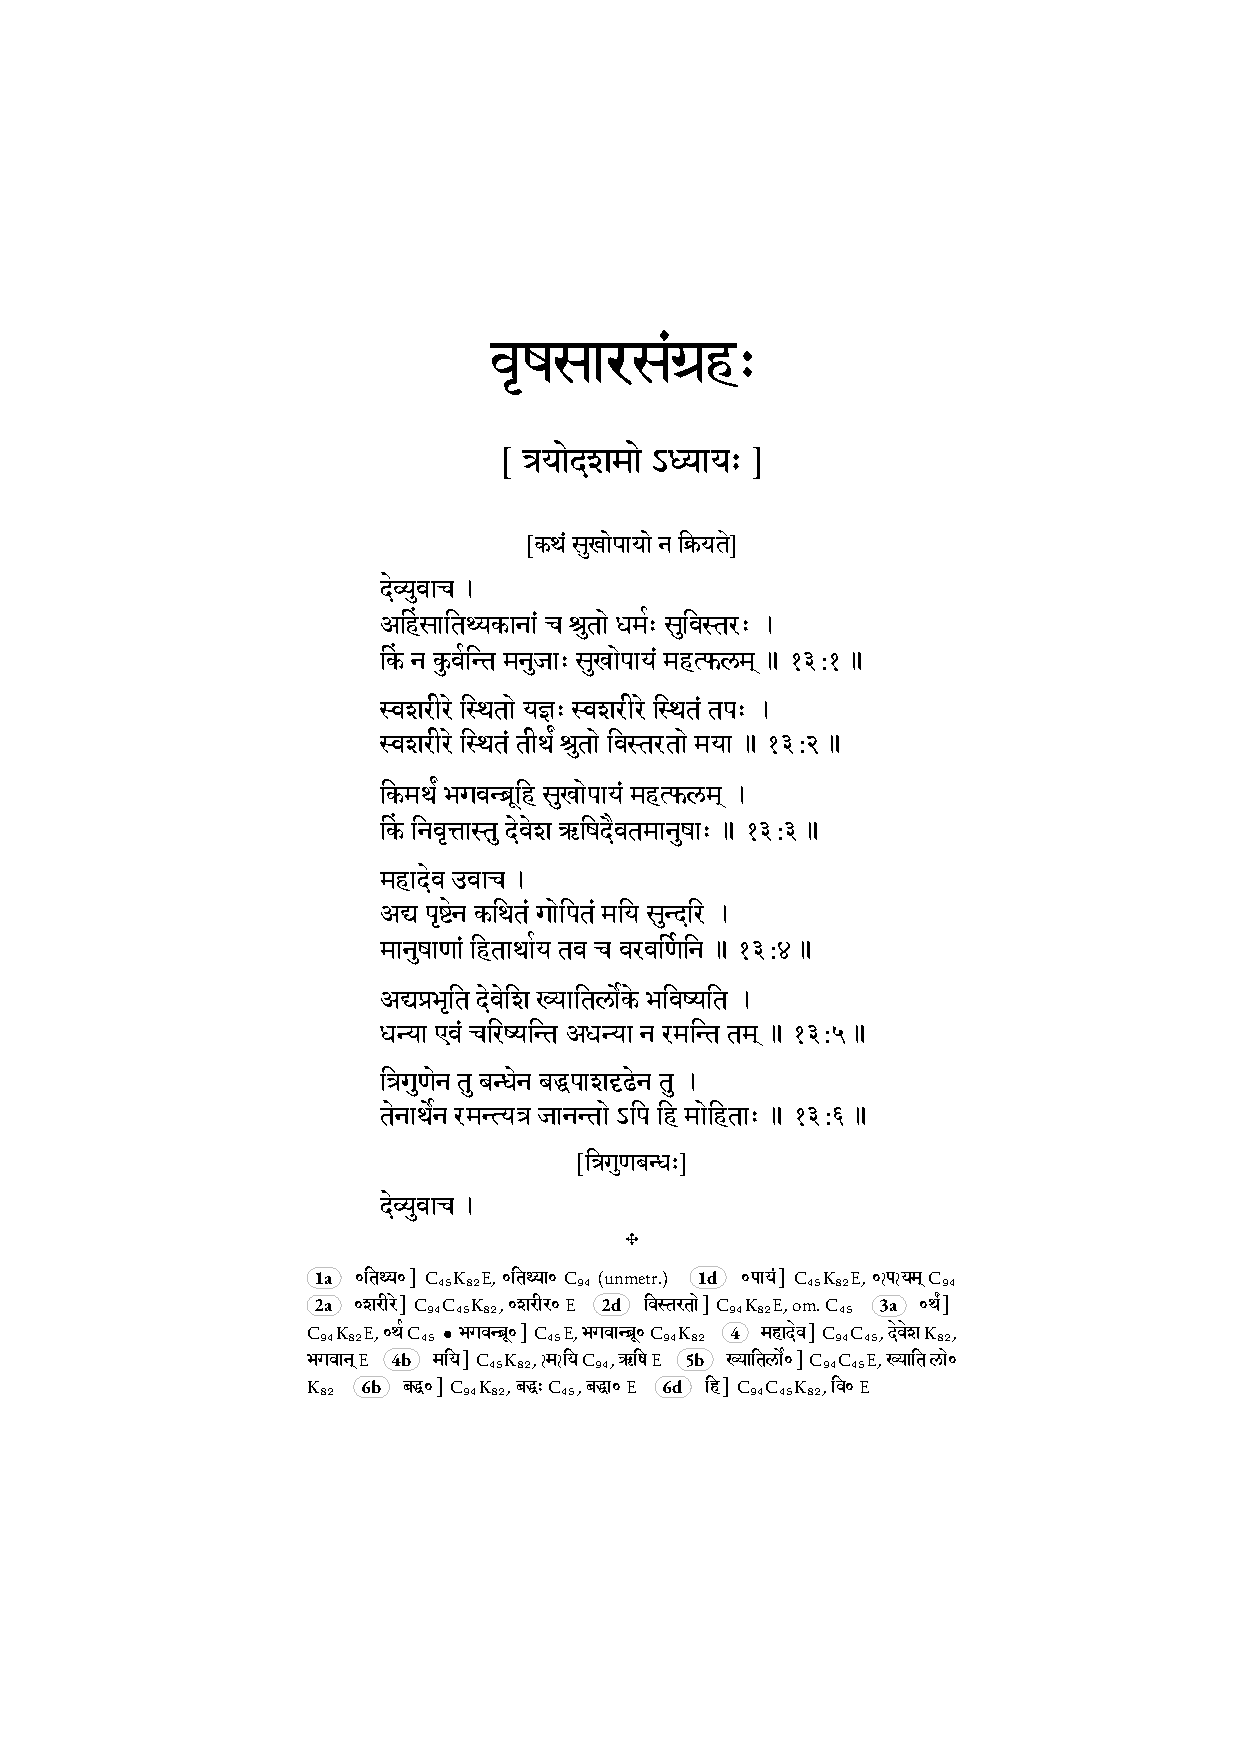
\includepdf[noautoscale, pages=-]{vrsasara_vol2_ed.pdf}




%%%%%%%%%%%%%%%
% TRANSLATION %
%%%%%%%%%%%%%%%


\mychapter{An Annotated Translation of Vṛṣasārasaṃgraha 13--24}
%\addcontentsline{toc}{section}{\Vss\ 1--12}


%FOOTNOTE
% Reformat footnotes
\makeatletter 
\renewcommand{\@makefntext}[1]{%
  \setlength{\parindent}{20pt}%
  %\begin{list}{}
  {\setlength{\labelwidth}{6mm}% 1.5em
    \setlength{\leftmargin}{0pt}%{\labelwidth}%
    \setlength{\labelsep}{10pt}%
    \setlength{\itemsep}{0pt}%
    \setlength{\parsep}{0pt}%
    \setlength{\topsep}{0pt}%
    \footnotesize}%
  %\item[\@thefnmark\hfil]
  #1% @makefnmark
  %\end{list}%
}
\makeatother 
\let\svthefootnote\thefootnote



\fancyhead[CE]{{\footnotesize \textit{Vṛṣasārasaṃgraha}}}
\fancyhead[CO]{{\footnotesize \textit{Translation of chapter 13}}}
%%%%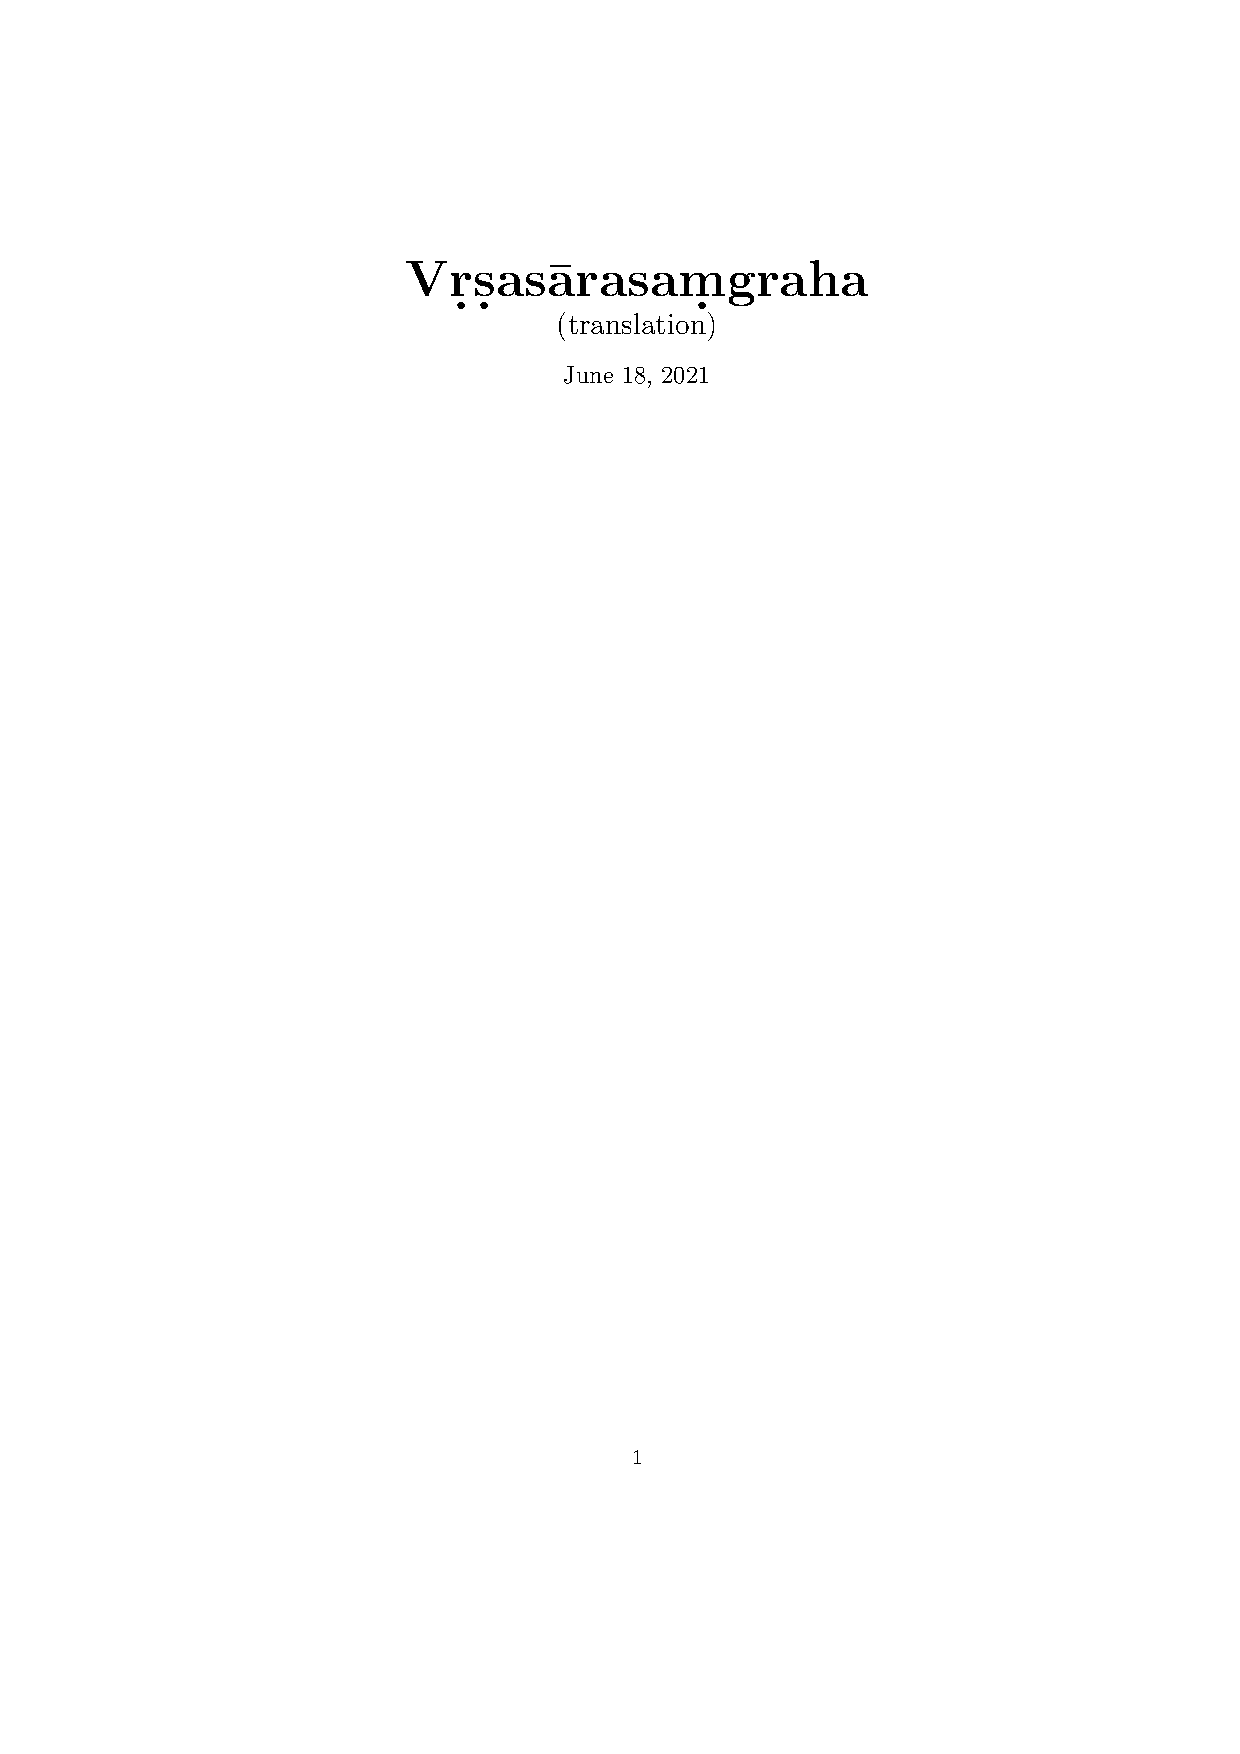
\includepdf[pages=-]{/home/csaba/indology/dharma_project/vrsa_edition/vss_translation.pdf}


% CORRECT PAGE NUMBER AFTER SKT EDITION !
\setcounter{page}{1001}
%%%%%% !TEX TS-program = xelatex
% !TEX encoding = UTF-8

% This is a simple template for a XeLaTeX document using the "article" class,
% with the fontspec package to easily select fonts.

\documentclass[11pt]{article} % use larger type; default would be 10pt

\usepackage{fontspec} % Font selection for XeLaTeX; see fontspec.pdf for documentation
\defaultfontfeatures{Mapping=tex-text} % to support TeX conventions like ``---''
\usepackage{xunicode} % Unicode support for LaTeX character names (accents, European chars, etc)
\usepackage{xltxtra} % Extra customizations for XeLaTeX

\setmainfont{Ariel} % set the main body font (\textrm), assumes Charis SIL is installed
%\setsansfont{Deja Vu Sans}
%\setmonofont{Deja Vu Mono}

% other LaTeX packages.....
\usepackage[width=12cm]{geometry} % See geometry.pdf to learn the layout options. There are lots.
\geometry{a4paper} % or letterpaper (US) or a5paper or....
%\usepackage[parfill]{parskip} % Activate to begin paragraphs with an empty line rather than an indent

\usepackage{graphicx} % support the \includegraphics command and options


\begin{document}

\textit{Qualities}

\end{document}


\
\pagebreak

\blankpage

\begin{center}{\huge\textbf{\englishfont Śivadharmaśāstra}}\end{center}\vskip2em
  \chptr{trayodaśamo 'dhyāyaḥ}
\fancyhead[CO]{{\footnotesize\textit{Translation of chapter 13}}}%

  \trchptr{Chapter Thirteen}
\fancyhead[CO]{{\footnotesize\textit{Translation of chapter 13}}}%

  \subchptr{kathaṃ sukhopāyo na kriyate}%

  \trsubchptr{Why is the easy method not followed?}%

  \maintext{devy uvāca |}%

  \maintext{ahiṃsātithyakānāṃ ca śruto dharmaḥ suvistaraḥ |}%

  \maintext{kiṃ na kurvanti manujāḥ sukhopāyaṃ mahat phalam }||\thinspace13:1\thinspace||%
\translation{Devī spoke: I have heard the Dharma of non-violence and of guest-reception in detail. Why do people not follow the easy method that brings about great rewards? \blankfootnote{13.1 \textit{Pāda}s ab and cd are back-references to chapters 12 and 11,
  respectively.
 }}

  \maintext{svaśarīre sthito yajñaḥ svaśarīre sthitaṃ tapaḥ |}%

  \maintext{svaśarīre sthitaṃ tīrthaṃ śruto vistarato mayā }||\thinspace13:2\thinspace||%
\translation{I have heard in full detail that worship resides in one's own body, and penance resides in one's body, and that the pilgrimage places reside in one's own body. \blankfootnote{13.2 \textit{Pāda}s ab and cd are back-references to chapters 11 and 10,
  respectively.
 }}

  \maintext{kimarthaṃ bhagavan brūhi sukhopāyaṃ mahat phalam |}%

  \maintext{kiṃ nivṛttās tu deveśa ṛṣidaivatamānuṣāḥ }||\thinspace13:3\thinspace||%
\translation{O Lord, tell me why does the easy method yields great rewards? And why are the sages, the gods, and the people indifferent? }

  \maintext{mahādeva uvāca |}%

  \maintext{adya pṛṣṭena kathitaṃ gopitaṃ mayi sundari |}%

  \maintext{mānuṣāṇāṃ hitārthāya tava ca varavarṇini }||\thinspace13:4\thinspace||%
\translation{Mahādeva spoke: Now, as I am asked to do so, I shall reveal the secret to you, O Sundarī, for the benefit of mankind and to favour you, O Varavarṇinī. \blankfootnote{13.4 Understand \textit{mayi} in \textit{pāda} b as \textit{mayā} metri causa.
 }}

  \maintext{adyaprabhṛti deveśi khyātir loke bhaviṣyati |}%

  \maintext{dhanyā evaṃ cariṣyanti adhanyā na ramanti tam }||\thinspace13:5\thinspace||%
\translation{From this day on, O Deveśī, it will be open knowledge {\rm (}\textit{khyāti}{\rm )} in the world. The fortunate ones will follow, the unfortunate ones will not delight in it. }

  \maintext{triguṇena tu bandhena baddhapāśadṛḍhena tu |}%

  \maintext{tenārthena ramanty atra jānanto 'pi hi mohitāḥ }||\thinspace13:6\thinspace||%
\translation{Because of the threefold bondage, in which the nooses are tied firmly, those who are stuck in it remain deluded, even if they are knowledgable. }

  \subchptr{triguṇabandhaḥ}%

  \trsubchptr{Threefold bondage}%

  \maintext{devy uvāca |}%

  \maintext{kiṃ vā triguṇabandheti brūhi saṃśayachedaka |}%

  \maintext{adyāpi mama deveśa mohotpannas tribandhanaiḥ }||\thinspace13:7\thinspace||%
\translation{Devī spoke: But what is this threefold bondage? Teach me, O you who repel my doubts. Even now, I am still confused, O Deveśa, by the threefold bondage. \blankfootnote{13.7 Understand \textit{mohotpannas} in \textit{pāda} d as
  \textit{moha utpannas} {\rm (}double sandhi{\rm )}.
 }}

  \maintext{bhagavān uvāca |}%

  \maintext{prākṛtaṃ vaikṛtaṃ caiva dakṣiṇābandham eva ca |}%

  \maintext{etenaiva tu bandhena baddhāḥ varṇāśramāḥ sadā }||\thinspace13:8\thinspace||%
\translation{The Lord spoke: The social classes {\rm (}\textit{varṇa}{\rm )} and the social order of disciplines {\rm (}\textit{āśrama}{\rm )} are bound forever by [1] natural {\rm (}\textit{prākṛta}{\rm )}, and [2] modified {\rm (}\textit{vaikṛta}{\rm )} bondage, and [3] the bondage of ritual reward {\rm (}\textit{dakṣiṇā\-bandha}{\rm )}. \blankfootnote{13.8 The three categories of \textit{prākṛta}- \textit{vaikṛta}- and \textit{dakṣiṇābandha} appear in commentaries on
  Sāṃkhya texts. One brief explanation that is close to what could be implied 
  here in the \VSS\ is Māṭhatavṛtti ad Sāṃkhyakārikā 44:
  \textit{tenājñānena manuṣyatiryagdeveṣv ātmānaṃ nibadhnāti\thinspace | na mokṣaṃ
  gacchatīty arthaḥ\thinspace | ato 'jñānaṃ nimittaṃ bandho naimittikāḥ\thinspace | sa ca bandhas
  trividhaḥ\thinspace | prakṛtibandho vaikārikabandho dakṣiṇābandhaś ceti\thinspace | tatra
  prakṛtibandho nāmāṣṭāsu prakṛtiṣu paratvenābhimānaḥ\thinspace | vaikārikabandho nāma
  brahmādisthāneṣu śreyobuddhiḥ\thinspace | dakṣiṇābandho nāma gavādidānejyānimittaḥ\thinspace |} 
 }}

  \maintext{jñānahīnā nivartante paramaṃ prāpya tat padam |}%

  \maintext{iṣṭastrīputrabhṛtyārthe dhanadhānyasamuccaye |}%

  \maintext{snehād ākṛṣṭamanasāṃ bandhaḥ prākṛta ucyate }||\thinspace13:9\thinspace||%
\translation{After they have reached that ultimate realm, being ignorant, [people] fall back for the sake of a desired woman, in order to have sons, servants, to accumulate money and grain. The bondage of minds that are caught by affection is called `natural' {\rm (}\textit{prākṛta}{\rm )}. }

  \maintext{yogayuktena manasā yad yad aiśvaryam āpyate |}%

  \maintext{tadā vaikṛtabandhaṃ tu yadi tatrānurajyate }||\thinspace13:10\thinspace||%
\translation{If one gets attached to the powers that one has obtained by controlling the mind with yoga, then it is the `modified' {\rm (}\textit{vaikṛta}{\rm )} bondage. }

  \maintext{ārāmodyānavāpīṣu dānakratuphaleṣu ca |}%

  \maintext{āsaktamanaso vāso dakṣiṇābandha kathyate }||\thinspace13:11\thinspace||%
\translation{The abiding[?] of one's mind that is attached to [donating] gardens, parks, and wells, to the fruits of donations and rites, is called the bondage of ritual reward {\rm (}\textit{dakṣiṇā\-bandha}{\rm )}. \blankfootnote{13.11 I have corrected °\textit{bandhaḥ} to °\textit{bandha}, a \stemform\ noun, in
  \textit{pāda} d to restore the metre.
 }}

  \maintext{anenaiva tu pāśena baddho vānaravad yathā |}%

  \maintext{mokṣituṃ na ca śaknoti itaś cetaś ca dhāvati }||\thinspace13:12\thinspace||%
\translation{Tied with this bondage, like monkeys not able to get away, people just keep running to and fro. }

  \maintext{devāsuramanuṣyeṣu tiryeṣu narakeṣu ca |}%

  \maintext{bhramate cakrayantravad yāvat tattvaṃ na vindati }||\thinspace13:13\thinspace||%
\translation{They will trasmigrate through [births among the] gods, demons, humans, animals, and in hells, as if on a wheel-machine, until they understand the truth. }

  \maintext{garbhavāsaparikleśo janmamṛtyuḥ punaḥ punaḥ |}%

  \maintext{vyādhiśokabhayāyāsacintayā jarayā hataḥ }||\thinspace13:14\thinspace||%
\translation{There is the pain of being in the womb, birth and death again and again, and then one dies of old age with anxiety about illness, sadness, danger, and fatigue. }

  \subchptr{garbhotpattiḥ}%

  \trsubchptr{Formation of the embryo}%

  \maintext{devy uvāca |}%

  \maintext{garbhotpattiḥ kathaṃ deva yogī labhati kīdṛśīm |}%

  \maintext{kīdṛśaṃ labhate garbhaṃ śrotuṃ naḥ pratidīyatām }||\thinspace13:15\thinspace||%
\translation{Devī spoke: How is the embryo produced, O god? And what kind [of development of an embryo] will the yogin go through? What kind of a womb will he end up? Allow us to hear this. }

  \maintext{bhagavān uvāca |}%

  \maintext{śṛṇu devi pravakṣyāmi garbhotpattiṃ yathākramam |}%

  \maintext{yathā saṃśayavicchedaṃ labhiṣyasi varānane }||\thinspace13:16\thinspace||%
\translation{Listen, O Devī, I shall teach you the formation of the embryo in due order, to put an end to your doubts, O Varānanā. }

  \maintext{akṣarāt prabhavo brahmā karma brahmasamudbhavam |}%

  \maintext{karmato yajñaprabhavo yajñato dhūmasambhavaḥ }||\thinspace13:17\thinspace||%
\translation{From the imperishable is born Brahmā. From Brahmā is born the ritual {\rm (}\textit{karman}{\rm )}. From ritual arises worship {\rm (}\textit{yajña}{\rm )}. From sacrifice arises smoke. \blankfootnote{13.17 Understand \textit{pāda} a as \textit{akṣarāt brahmaprabhavaḥ}.
 \textit{Pāda} c is a \textit{na-vipulā} if the syllabe \textit{pra}
  does not makes the previous syllable heavy {\rm (}\mutacumliquida{\rm )}.
 }}

  \maintext{dhūmrād abhrāṇi jāyante abhrāt parjanyasambhavaḥ  |}%

  \maintext{parjanyād annam{-}utpattir annād bhūtāni jajñire }||\thinspace13:18\thinspace||%
\translation{From smoke are born the clouds. From the clouds come the rain-clouds. From the rain-clouds food arises. From food living beings arise. \blankfootnote{13.18 Understand \textit{annam utpattir} in \textit{pāda} c as a \textit{tatpuruṣa} compound.
 }}

  \maintext{annād rasasamutpattī rasāc choṇitasambhavaḥ |}%

  \maintext{śoṇitān māṃsam{-}utpattir māṃsād medasamudbhavaḥ }||\thinspace13:19\thinspace||%
\translation{From food arises flavour {\rm (}\textit{rasa}{\rm )}. From flavour arises blood. From blood flesh arises. From flesh fat arises. }

  \maintext{medaso 'sthīni jāyante asthibhyo majjasambhavaḥ |}%

  \maintext{majjāyās tu bhavec chukraṃ naraḥ śukrasamudbhavaḥ }||\thinspace13:20\thinspace||%
\translation{From fat bones arise. From the bones marrow arises. From marrow arises semen. And man is born from semen. }

  \maintext{śukraśoṇitasaṃyogād garbhotpattis tataḥ smṛtā |}%

  \maintext{agnisomātmakaṃ devi śarīraṃ dvayadhātutaḥ }||\thinspace13:21\thinspace||%
\translation{The formation of the embryo is known to come from the union of semen and blood. The body is made of Fire and Soma, O Devī, because of the two [corresponding] elements. }

  \maintext{somadhātu smṛtaṃ śukram agnidhātu rajaḥ smṛtam |}%

  \maintext{agnisomāśrayaṃ devi śarīram iti saṃjñitam }||\thinspace13:22\thinspace||%
\translation{Semen is said to be of the Soma element, blood is said to be of the Fire element. The body is taught to be the seat of Fire and Soma, O Devī. }

  \maintext{māse māse ṛtuḥ strīṇāṃ bhavatīha na saṃśayaḥ |}%

  \maintext{ṛtukāle prasarpeta na sukhārthaṃ varānane }||\thinspace13:23\thinspace||%
\translation{Each month women have their periods, no doubt about it. One should approach them at the time of their period, and not for pleasure, O Varānanā. }

  \maintext{putrakāmaḥ prayuñjīta dharmārthaṃ ca yaśasvini |}%

  \maintext{pumān strīṣūpayuñjīta araṇīva hutāśanam }||\thinspace13:24\thinspace||%
\translation{One should enjoy [a woman] if one wishes to have a son, and for the sake of religious duty {\rm (}\textit{dharma}{\rm )}, O Yaśasvinī. The man should enjoy the women[, and produce offspring,] like two sticks [rubbed together produce] fire. }

  \maintext{pumān śukrādhiko jñeyaḥ kanyā raktādhikā bhavet |}%

  \maintext{samaśukre ca rakte ca sa ca jāyen napuṃsakaḥ }||\thinspace13:25\thinspace||%
\translation{Males are to be known as having an excess of semen, while females have an excess of blood. When the semen and the blood are in equal quantitiy, a gender-neutral [child] will be born. }

  \subchptr{dviyamā triyamā ca gurviṇī}%

  \trsubchptr{Pregnancy with twins and triplets}%

  \maintext{devy uvāca |}%

  \maintext{dviyamā triyamā caiva kathaṃ jāyeta gurviṇī |}%

  \maintext{kathaṃ strīdviyamā jāyet kathaṃ vā puruṣadvayam }||\thinspace13:26\thinspace||%
\translation{Devī spoke: How does a woman become pregnant with twins or triplets? How are twin girls born and how are twin boys born? }

  \maintext{bhagavān uvāca |}%

  \maintext{raktādhikā smṛtā kanyā jāyate varavarṇini |}%

  \maintext{vāyunā ca dvidhā bhinnā kanyakādviyamā smṛtā }||\thinspace13:27\thinspace||%
\translation{The Lord spoke: When there is an excess of blood, a daughter is born, O Varavarṇinī. When it is split into two by Wind, it will be twin girls. }

  \maintext{śukrādhikas tu puruṣo dvidhā bhinno 'nilena tu |}%

  \maintext{dviyamā puruṣā jñeyās triyamās tu tridhā kṛte }||\thinspace13:28\thinspace||%
\translation{And when the male, which has an excess of semen, is split into two by Wind, they will be twin boys. When it is split into three, they will be triplets. }

  \maintext{ṛtusnātā yadā nārī yadi garbhād vigṛhṇati |}%

  \maintext{prathame ca dvitīye ca tṛtīye ca na jīvati }||\thinspace13:29\thinspace||%
\translation{When a woman has just bathed after her period, if she conceives[?] in[?] her womb on the first, second, or third day, [the embryo] will not survive. }

  \maintext{sameṣu janayet putraṃ kanyakāṃ viṣame dine |}%

  \maintext{ṣaṣṭy aṣṭamī ca daśamī dvādaśī ca pumān bhavet }||\thinspace13:30\thinspace||%
\translation{On even days, he will beget a son, on odd days, a daughter. On the sixth, eighth, tenth, and twelfth days: it will be a male. }

  \maintext{pañcamī saptamī caiva navamy ekādaśī striyaḥ |}%

  \maintext{samarakte ca śukre ca śyāmaḥ saṃjāyate pumān }||\thinspace13:31\thinspace||%
\translation{On the fifth, seventh, ninth, and eleventh days: a female. When blood and semen are even, the man will be dark-coloured. }

  \maintext{rudhiraṃ tv ekarātreṇa kalalaṃ pratipadyate |}%

  \maintext{kalalaṃ pañcarātreṇa arbudatvaṃ prajāyate }||\thinspace13:32\thinspace||%
\translation{The blood will turn into a spot in one day. This spot will become a lump in five days. }

  \maintext{arbudaḥ saptarātreṇa māṃsapeśīsamudbhavaḥ |}%

  \maintext{dvitīyasaptarātreṇa tat sarvaṃ māṃsaśoṇitam }||\thinspace13:33\thinspace||%
\translation{The lump will become a piece of flesh by the end of the first week. By the end of the second week, the whole thing will be flesh and blood. }

  \maintext{tṛtīyasaptarātreṇa hṛdayaṃ jāyate tataḥ |}%

  \maintext{tataḥ sarvāṇi gātrāṇi śiraś caivopajāyate }||\thinspace13:34\thinspace||%
\translation{By the end of the third week, it will have a heart. Then all the limbs and the head are formed. }

  \maintext{hṛdaye jāyamāne tu mūrcchā tandrir arocakaḥ |}%

  \maintext{striyāś chardiḥ prasekaś ca daurbalyaṃ copajāyate }||\thinspace13:35\thinspace||%
\translation{When the heart is developing, [the women will experience] fainting, exhaustion, and loss of apetite. She will experience nausea, vomiting and weakness. }

  \maintext{tasya hi hṛdayaṃ nārī yadi bhidyati kiṃcana |}%

  \maintext{bhakṣyaṃ lehyaṃ tathā peyam upabhogāṃs tathārthayet }||\thinspace13:36\thinspace||%
\translation{If the woman's heart is longing for something, and she asks for any food, be it chewable, sippable, drinkable, or any kind of delicacy, \blankfootnote{13.36 The translation of this verse is tentative and presupposes
  that the construction \textit{tasya ... hṛdayaṃ nārī} stands for
  \textit{tasyā nāryā hṛdayaṃ}. Perhaps understand \textit{bhidyati} 
  in \textit{pāda} b as \textit{bhedayati} {\rm (}causative{\rm )}.
 }}

  \maintext{śayanāsanadānāni vastrāṇy ābharaṇāni ca |}%

  \maintext{yad yad ākāṅkṣate kiṃcit tadāsyaiva pradāpayet }||\thinspace13:37\thinspace||%
\translation{a bed, a seat, gifts, clothes, or jewellery, anything she desires, one should give that to her immediately. \blankfootnote{13.37 Perhaps understand \textit{tadāsyaiva} {\rm (}or \textit{tad asyaiva}{\rm )} 
  as \textit{tadaiva asyai} {\rm (}or \textit{tad eva asyai}{\rm )}.
 }}

  \maintext{nāyāsaṃ kārayec cāsyā na caivam avamānayet |}%

  \maintext{mukham āpāṇḍuraṃ snigdhaṃ kālatvaṃ stanakakṣayoḥ }||\thinspace13:38\thinspace||%
\translation{One should not cause her trouble, and should not ignore her. Her face is pale and greasy, her breasts and armpits dark. }

  \maintext{śarīraṃ ca śriyā juṣṭaṃ pīnoruśroṇivaṅkṣaṇam |}%

  \maintext{liṅgair ebhir vijānīyād garbhe jīvaṃ pratiṣṭhitam }||\thinspace13:39\thinspace||%
\translation{Her body is inhabited by beauty, her thighs, buttocks, and groin are round and fleshy. By these sings, one should know that there is a [new] life in the womb. }

  \maintext{caturthasaptarātreṇa śiraś caivopajāyate |}%

  \maintext{pañcamasaptarātreṇa grīvā tatropajāyate }||\thinspace13:40\thinspace||%
\translation{By the fourth week, the head develops. By the fifth week, the neck develops. }

  \maintext{ṣaṣṭhamasaptarātreṇa skandhagātraṃ prajāyate |}%

  \maintext{saptamasaptarātreṇa pṛṣṭhavaṃśaḥ prajāyate }||\thinspace13:41\thinspace||%
\translation{By the sixth week, the shoulders and the limbs form. By the seventh week, the backbone develops. }

  \maintext{aṣṭamasaptarātreṇa pāṇī jāyata cobhayau |}%

  \maintext{saptarātraṃ nava prāpya jāyate hy urapañjaram }||\thinspace13:42\thinspace||%
\translation{By the eighth week, the two hands form. By the ninth week, the ribs develop. \blankfootnote{13.42 I conjecture \textit{jāyata} {\rm (}for a standard \textit{parasmaipada} dual \textit{jāyataḥ}{\rm )} in \textit{pāda} b,
  influenced by \msCb's reading in 13.43b, to restore the metre.
 }}

  \maintext{daśame saptarātre ca pādau jāyata cobhau |}%

  \maintext{udaraṃ copajāyeta saptaikādaśarātrike }||\thinspace13:43\thinspace||%
\translation{By the tenth week, the two feet develop. By the eleventh week, the abdomen forms. }

  \maintext{dvādaśasaptarātreṇa kukṣipārśvaḥ prajāyate |}%

  \maintext{saptatraidaśarātreṇa kaṭis tatropajāyate }||\thinspace13:44\thinspace||%
\translation{By the twelfth week, the flanks of the abdomen form. By the thirteenth week, its buttocks develop. }

  \maintext{navaty aṣṭa ca rātreṇa jāyate sūtraviṃśatiḥ |}%

  \maintext{saptapañcadaśāhena sarvamedaḥ prajāyate }||\thinspace13:45\thinspace||%
\translation{By the ninety-eighth night [i.e.\ by the fourteenth week], the ten fingers and ten toes develop. By the fifteenth week, all the fat is developed. \blankfootnote{13.45 The word \textit{sūtra} is unusual in the sense of `a finger/toe'.
  I base my translation on \SDHU\ 8.32cd, which seems to 
  point to the same period of pregnancy:
  \textit{māsaiś caturbhir aṅgulyaḥ prajāyante yathākramam};
  `By the fourth month the fingers develop in due order.'
 }}

  \maintext{ṣoḍaśasaptarātreṇa asthi sarvāṇi jāyate |}%

  \maintext{saptasaptadaśāhena jāyate snāyubandhanam }||\thinspace13:46\thinspace||%
\translation{By the sixteenth week, all the bones are formed. By the seventeenth week, the sinews are fixed. }

  \maintext{saptamāṣṭādaśāhena jāyate mukhamaṇḍalam |}%

  \maintext{saptonaviṃśarātreṇa ghrāṇavaṃśaḥ prajāyate }||\thinspace13:47\thinspace||%
\translation{By the eighteenth week, the face develops. By the nineteenth week, the nasal canal is formed. }

  \maintext{saptaviṃśatirātreṇa netranālaṃ prajāyate |}%

  \maintext{saptaikaviṃśarātreṇa karṇayugmaṃ prajāyate }||\thinspace13:48\thinspace||%
\translation{By the twentieth week, the veins of the eye develop. By the twenty-first week, the two ears form. }

  \maintext{dvāviṃśasaptarātreṇa jāyate dvau bhruvau tataḥ |}%

  \maintext{saptatriviṃśarātreṇa gaṇḍayugmaṃ prajāyate }||\thinspace13:49\thinspace||%
\translation{By the twenty-second week, the two eyebrows form. By the twenty-third week, the two cheeks develop. }

  \maintext{caturviṃśatisaptāhe oṣṭhayugmaṃ prajāyate |}%

  \maintext{pañcaviṃśatisaptāhe jihvā jāyeta sundari }||\thinspace13:50\thinspace||%
\translation{By the twenty-fourth week, the two lips develop. By the twenty-fifth week, the tongue is born, O Sundarī. }

  \maintext{ṣaḍviṃśasaptarātreṇa dantapālī prajāyate |}%

  \maintext{saptaviṃśatisaptāhe jāyate vṛṣaṇadvayam }||\thinspace13:51\thinspace||%
\translation{By the twenty-sixth week, the gums develop. By the twenty-seventh week, the testicles form. }

  \maintext{aṣṭāviṃśatisaptāhe bhagaliṅgaṃ prajāyate |}%

  \maintext{ūnaviṃśatisaptāhe jāyate ca tvag eva ca }||\thinspace13:52\thinspace||%
\translation{By the twenty-eighth week, the womb and the penis develop. By the twenty-ninth week, the skin forms. }

  \maintext{triṃśatisaptarātreṇa jāyate nābhimaṇḍalam |}%

  \maintext{saptaikatriṃśarātreṇa sarvarandhraṃ prajāyate }||\thinspace13:53\thinspace||%
\translation{By the thirtieth week, the navel develops. By the thirty-first week, all the cavities are formed. }

  \maintext{dvātriṃśatsaptarātreṇa nakhaviṃśati jāyate |}%

  \maintext{tretriṃśatsaptarātreṇa roma keśaś ca jāyate }||\thinspace13:54\thinspace||%
\translation{By the thirty-second week, the twenty nails are formed. By the thirty-third week, hair on the body and on the head grow. \blankfootnote{13.54 Note °\textit{viṃśati} for °\textit{viṃśatir} in \textit{pāda} b metri causa.
 }}

  \maintext{saptarātracatustriṃśe sarvasandhiḥ prajāyate |}%

  \maintext{pañcatriṃśatisaptāhe sarvamarma prajāyate }||\thinspace13:55\thinspace||%
\translation{By the thirty-fourth week, all the joints are formed. By the thirty-fifth week, all the \textit{marman}-joints are formed. }

  \maintext{ṣaḍtriṃśasaptarātreṇa vedanā copajāyate |}%

  \maintext{saptatriṃśatisaptāhe īrṣādveṣaḥ prajāyate }||\thinspace13:56\thinspace||%
\translation{By the thirty-six week, consciousness arises. By the thirty-seventh week, envy and hatred arise. }

  \maintext{aṣṭatriṃśatisaptāhe pañcātmakasamanvitam |}%

  \maintext{sarvāṅgam aṅgasampūrṇaḥ paripakvaḥ sa tiṣṭhati }||\thinspace13:57\thinspace||%
\translation{By the thirty-eighth week, being composed of the five elements {\rm (}\textit{pañcātmaka}{\rm )}, having all limbs and a full body, it is fully developed. }

  \maintext{mātuḥ śvāśitapītaṃ ca nābhisūtrāgamena tu |}%

  \maintext{prajātasyopadhāryante garbhasthasyaiva jantavaḥ }||\thinspace13:58\thinspace||%
\translation{It is breathing and drinking from the mother, from a flow [of nutrients] through the umbilical cord. Humans nourish a child that has been born just as they do a baby in the womb. \blankfootnote{13.58 The translation of \textit{pāda}s cd is tentative. I take 
  \textit{upadhāryante} as a causative {\rm (}\textit{upadhārayanti}{\rm )}.
 }}

  \maintext{tataḥ praviśate cittaṃ nidrāsvapnaṃ yathā tathā |}%

  \maintext{nopalabhyati sūkṣmatvād araṇy agnir yathā tathā }||\thinspace13:59\thinspace||%
\translation{Then consciousness enters the mind, as if sleep and dream. It cannot [be?] perceived because of its subtlety, like the fire [that resides inside] the sticks [that produce fire cannot be seen?]. }

  \maintext{garbhodakena siktāṅgo jarāyupariveṣṭitaḥ |}%

  \maintext{jātiṃ smarati tatrastho jantuś cetaḥsamanvitaḥ }||\thinspace13:60\thinspace||%
\translation{Wet with the amniotic fluid, he is surrounded by the fetal membranes. Being in there, the child, now being conscious, starts remembering [previous] births. }

  \maintext{mṛtaś cāhaṃ punarjāto bhūyaś caiva punar mṛtaḥ |}%

  \maintext{sthāvarāṇāṃ sahasreṣu jāto 'smi vividheṣu ca }||\thinspace13:61\thinspace||%
\translation{`I died and was then reborn. And then I died again. I was reborn in thousands of different plants, }

  \maintext{tiryagyonisahasreṣu preteṣu narakeṣu ca |}%

  \maintext{caturvarṇavivarṇeṣu mānuṣeṣu sahasraśaḥ }||\thinspace13:62\thinspace||%
\translation{in thousands of animals, as ghosts in hells, as thousands of humans in the four main social classes {\rm (}\textit{varṇa}{\rm )} and in mixed castes. }

  \maintext{sāmprataṃ ca punar garbhaḥ kleśaprāptaḥ suduḥsahaḥ |}%

  \maintext{idānīṃ jātamātro 'haṃ saṃskāraiś cāpi saṃskṛtaḥ }||\thinspace13:63\thinspace||%
\translation{And now I am again an embryo, in unbearable anguish. Now I am a newborn baby, being purified by rituals {\rm (}\textit{saṃskāra}{\rm )}. }

  \maintext{yogam evābhisevāmi sāṃkhyaṃ vā pañcaviṃśakam |}%

  \maintext{yatra janmajarā nāsti yatra mṛtyuś ca nāsti vai }||\thinspace13:64\thinspace||%
\translation{I will do nothing but practise yoga or the Sāṃkhya of twenty-five [\textit{tattva}s]. Where there is no birth and no aging, and where there is no death, }

  \maintext{yatra brahma paraṃ vaidyaṃ cariṣyāmi yatavrataḥ |}%

  \maintext{evam ādīny anekāni cintayitvā punaḥ punaḥ }||\thinspace13:65\thinspace||%
\translation{where the Brahman is the ultimate doctor, I shall go there, keeping my vows firmly.' It thinks about these and many similar things again and again. \blankfootnote{13.65 That the \textit{brahman} is the ultimate doctor {\rm (}\textit{vaidyaṃ}{\rm )} or
  something to be known {\rm (}\textit{vedyaṃ}{\rm )} here is debateble.
  I have chosen the former as a sort of lectio difficilior.
 }}

  \maintext{yāvat tiṣṭhati garbhastho jātiṃ smarati pūrvikām |}%

  \maintext{tato jāyati kaṣṭena mahākleśena mānavaḥ }||\thinspace13:66\thinspace||%
\translation{While in the womb, it remembers its previous births. Then the human is born with great difficulty and great pain, }

  \maintext{yoniyantrasutīvreṇa pīḍyamānaḥ suduḥkhitaḥ |}%

  \maintext{jātamātre smṛtibhraṃśo bhavatīha acetanaḥ }||\thinspace13:67\thinspace||%
\translation{tormented by the mechanisms of the vagina, in incredible pain. As soon as it is born, it forgets its [previous] lives in this world, unconscious. }

  \maintext{māyāmudgaratīvreṇa hataḥ kiṃ śubham ācaret |}%

  \maintext{eṣa garbhasamutpattiḥ kathito 'smi varānane |}%

  \maintext{duḥkhasaṃsāraprathamaḥ kiṃ bhūyaḥ śrotum icchasi }||\thinspace13:68\thinspace||%
\translation{[The baby] is hit by the hard hammer of illusion {\rm (}\textit{māyā}{\rm )}. How could it act in an auspicious way? This is how I have told you the formation of the embryo, O Varānanā, the first [stage] of the suffering in transmigration {\rm (}\textit{saṃsāra}{\rm )}. What else would you like to hear? \blankfootnote{13.68 In fact, 13.68 in \msCa, \msCb, and \msNa\ end with \textit{icchasīti}, 
  leading into the colophon {\rm (}\textit{vṛṣasārasaṃgrahe...}{\rm )}, but \msCb\
  repeats the \textit{iti} thus: \textit{icchasīti\thinspace || iti vṛṣasārasaṃgrahe...}
 }}

\centerline{\maintext{\dbldanda\thinspace iti vṛṣasārasaṃgrahe garbhotpattir{ }adhyāyas{ }trayadaśamaḥ\thinspace\dbldanda}}
\translation{Here ends the thirteenth chapter in the \textit{Vṛṣasārasaṃgraha} chapter on The development of the embryo.}

  \chptr{caturdaśamo 'dhyāyaḥ}
\fancyhead[CO]{{\footnotesize\textit{Translation of chapter 14}}}%

  \trchptr{Chapter Fourteen}%

  \subchptr{deharūpavarṇabhedāni}%

  \trsubchptr{Differences in body-shapes and skin-colours}%

  \maintext{devy uvāca |}%

  \maintext{atidīrgho 'tihrasvaś ca pumān kenopajāyate |}%

  \maintext{atigauro 'tikṛṣṇaś ca naro bhavati kiṃ prabho }||\thinspace14:1\thinspace||%
\translation{Devī spoke: How does a person become extremely tall or very short? Why does one person have an extremely fair complexion, and the other a very dark one, O Lord? }

  \maintext{bhagavān uvāca |}%

  \maintext{gṛhītagarbhā yā nārī nityam uttānaśālinī |}%

  \maintext{prasāritavibhaktātmā so 'tidīrghaḥ prajāyate }||\thinspace14:2\thinspace||%
\translation{The Lord spoke: If a pregnant woman always stands upright, the son will have an expanded and symmetrical body, and will be extremely tall. }

  \maintext{gṛhītagarbhā yā nārī śete saṃkucitā sadā |}%

  \maintext{rasānnādīni kaṭukaṃ sevanā hrasva jāyate }||\thinspace14:3\thinspace||%
\translation{If a pregnant woman always lies down in a contracted posture, [and] indulges in pungent juices and food, the son will be short. \blankfootnote{14.3 Understand \textit{pāda} c as \textit{rasānnādīni kaṭukāni}, and 
  note the stem-form word \textit{hrasva} metri causa in \textit{pāda} d.
 }}

  \maintext{gṛhītagarbhā yā nārī nityaṃ kṣīropasevinī |}%

  \maintext{varakodravaśālīṃś ca bhuṅkte cāpi yavaudanam |}%

  \maintext{śuklavastrasrajā yuktā sātigauraṃ prasūyate }||\thinspace14:4\thinspace||%
\translation{If a pregnant woman always drinks milk, eats \textit{vara} and \textit{kodrava} grains, and rice, and barley-porrige, wears white clothes and white garlands, she will give birth to [offspring] with extremely pale complexion. }

  \maintext{gṛhītagarbhā yā nārī kāladhānyāni sevate |}%

  \maintext{māṣakṛṣṇatilāmudgaṃ tathā kṛṣṇayavodanam |}%

  \maintext{kṛṣṇavastrasrajādīni tasyāḥ kṛṣṇaḥ prajāyate }||\thinspace14:5\thinspace||%
\translation{If a pregnant woman loves black-coloured grains, black beans, black sesamum, black Mungo beans, and porridge made of black barley, [and wears] dark clothes and garlands, she will have a son with dark skin. }

  \subchptr{jātidoṣāni}%

  \trsubchptr{Birth defects}%

  \maintext{devy uvāca |}%

  \maintext{jātyandho jāyate kasmāt ṣaṇḍho bhīrur hatendriyaḥ |}%

  \maintext{kubjo vā vāmano vāpi paṇḍaḥ sthūlaśiraḥ katham }||\thinspace14:6\thinspace||%
\translation{Devī spoke: Why is a person born blind, gender-neutral, timid, with ruined sense-faculties, hump-backed, dwarfish, a weakling, or with an enourmous head? }

  \maintext{bhagavān uvāca |}%

  \maintext{gṛhītagarbhā yā nārī tīkṣṇoṣṇāny upasevate |}%

  \maintext{laśunāni palāṇḍūni karañjamūlakāni ca }||\thinspace14:7\thinspace||%
\translation{The Lord spoke: If a pregnant woman indulges in hot and pungent [food], in garlic and onion, the root of the wood-apple tree, }

  \maintext{pippalīṃ śṛṅgaveraṃ ca sarṣapān maricāni ca |}%

  \maintext{āsavaṃ ca parikliṣṭā ye cānye kaṭutiktakāḥ |}%

  \maintext{tīkṣṇaṃ tu sevamānā yā jātyandhaṃ janayet sutam }||\thinspace14:8\thinspace||%
\translation{berries, ginger, mustard, and black pepper, alcohol, and other [types of] harmful[?], pungent and bitter [food], [i.e.] she who enjoys hot [food], will give birth to a blind child. }

  \maintext{mithyopacārāḥ strīpuṃso vyāpanne śukraśoṇite |}%

  \maintext{yadā garbhāśaye raktaṃ striyāḥ pūrvaṃ niṣicyate |}%

  \maintext{paścāc chukraṃ raktakāle tadā ṣaṇḍaḥ prasūyate }||\thinspace14:9\thinspace||%
\translation{[If] the conduct[?] of the woman and the man is improper, the semen and blood are spoiled. When the woman's blood flows into the womb first, at the time of her period???, and then the semen, then a gender-neutral child will be born. }

  \maintext{trastodvignā yadā bhītā strī puṃsā sūyate prajā |}%

  \maintext{tatra yo jāyate garbhād bhīruḥ krandanako bhavet }||\thinspace14:10\thinspace||%
\translation{When a woman is frightened, terrified, afraid of the man, and offspring is conceived, then what is born from her womb will be a coward, a crybaby. \blankfootnote{14.10 puṃsāṃ is odd
 }}

  \maintext{visargakāle śukrasya vighna utpadyate yadā |}%

  \maintext{indriyāvartavighne tu tadā jāyed anindriyaḥ }||\thinspace14:11\thinspace||%
\translation{Should any obstacle arise in front of the semen at the moment of ejaculation, then [the child] will be born without any sense faculties because of the blocking of the development of the senses[????]. }

  \maintext{gṛhītagarbhā yā nārī vātalāny upasevate |}%

  \maintext{kaṭukāni kaṣāyāni tiktāni ca viśeṣataḥ }||\thinspace14:12\thinspace||%
\translation{If a pregnant woman indulges in eating pulses, in pungent, astringent, and especially, bitter [food], }

  \maintext{vātaḥ prakupitas tasyā garbham ābhujya tiṣṭhati |}%

  \maintext{kubjas tu jāyate tasmād garbhād vātanipīḍanāt }||\thinspace14:13\thinspace||%
\translation{her \textit{vāta} humour will be agitated, and it will be pressing down the womb. A hump-backed child will be born from that womb because of the compression of \textit{vāta}. }

  \maintext{nityam āsanaśīlā yā tathā cotkuṭakāsanā |}%

  \maintext{tasyāḥ saṃhanyate garbho vāmanas tena jāyate }||\thinspace14:14\thinspace||%
\translation{She who is always sitting or squatting will crush the embryo, which will by this be born a dwarf. }

  \maintext{ativyāyāmaśīlā tu yā nārī viṣamāsanī |}%

  \maintext{garbhaḥ saṃkṣubhyate tasyāḥ paṇḍas tenopajāyate }||\thinspace14:15\thinspace||%
\translation{If a woman exercises too much, [or often] sits in an unbalanced way, her womb will be shaken, and by this a weakling will be born. }

  \maintext{gṛhītagarbhā yā nārī rūḍhadhānyāni sevate |}%

  \maintext{vātaśleṣma śirastho vai tasya garbhasya kupyate |}%

  \maintext{tataḥ sthūlaśirās tena pumān jāyaty asaṃśayaḥ }||\thinspace14:16\thinspace||%
\translation{If a pregnant woman indulges in grain that is sprouting[?], the Wind and Phlegm in the the embryo's head will swell up. Then, because of this, a man with an enormous head will be born, no doubt. }

  \maintext{devy uvāca |}%

  \maintext{karālāṅgā hanuḥ paṅgur mūko gadgadabhāṣakaḥ |}%

  \maintext{vivṛtākṣas tv anakṣo vā bhaved duḥkhagudaḥ katham }||\thinspace14:17\thinspace||%
\translation{Devī spoke: How can [a person] be born with terrible limbs, with a terrible jaw[?], as lame, a mute, stammering, [always] open-eyed, or eyeless, or having a painful anus? }

  \maintext{bhagavān uvāca |}%

  \maintext{karālastanadoṣeṇa jāyate mānavas tathā |}%

  \maintext{atha karālaṃ kurute nārī lamboticūcukā |}%

  \maintext{tasmād etena doṣeṇa karālo jāyate pumān }||\thinspace14:18\thinspace||%
\translation{The Lord spoke: It is by the fault of [the mother's] having terrible[?] breasts that a man is born like that [i.e. with terrible limbs]. Now, a woman with extremely dangling nipples does terrible things[???]. Therefore, by this fault, a terrible man is born. }

  \maintext{gṛhītagarbhā yā nārī raktapittāmayārditā |}%

  \maintext{gohanuṃ janayaty eṣā raktapittaprakopitā }||\thinspace14:19\thinspace||%
\translation{If a pregnant woman is afflicted by diseases of the blood and the Pitta, having her blood and Pitta irritated, she will give birth to a child with a cow's jaw[??]. }

  \maintext{gṛhītagarbhā yā nārī vātaśūlair upadrutā |}%

  \maintext{śukrodāvartanī cāpi paṅguṃ janayate sutam }||\thinspace14:20\thinspace||%
\translation{If a pregnant woman is pained by flatulence, or retains her menstrual discharge, she will give birth to a lame child. }

  \maintext{kṣudhārtā vedanārtā ca satataṃ copavāsinī |}%

  \maintext{mūkaṃ janayate putraṃ dauhṛdaṃ ca vimānitā }||\thinspace14:21\thinspace||%
\translation{If she is afflicted by thirst and pain, and always fasts, she will give birth to a mute, her longings of pregnancy {\rm (}\textit{dauhṛda}{\rm )} having been refused. \blankfootnote{14.21 Cf. Suśruta 3.3.21:
  \textit{yeṣu yeṣv indriyārtheṣu dauhṛde vai vimānanā\thinspace |
  prajāyeta sutasyārtis tasmiṃst asmiṃs tathendriye||.}
  Yājñavalkya 3.79:
  \textit{dauhṛdasyāpradānena garbho doṣam avāpnuyāt\thinspace |
  vairūpyaṃ maraṇaṃ vāpi tasmāt kāryaṃ priyaṃ striyāḥ\thinspace ||}
 }}

  \maintext{gṛhītagarbhā yā nārī visṛjen māsamāsikam |}%

  \maintext{anakṣo jāyate tasyā garbhaśoṇitasaṃkṣayāt }||\thinspace14:22\thinspace||%
\translation{If a pregnant woman discharges [menstrual blood] every month, she will give birth to a blind child due to the damage made by the blood to the embryo. }

  \maintext{arśagrastā yadā nārī vātodāvartapīḍitā |}%

  \maintext{gṛhītagarbhā rūkṣāṇi vātalāny upasevate }||\thinspace14:23\thinspace||%
\translation{If a pregnant woman is afflicted by h\ae morrhoids, and is pained by bowel diseases caused by Wind {\rm (}\textit{vāta}{\rm )}, and indulges in astringent [foods and?] pulses, }

  \maintext{vātasthānaṃ tatas tasyā garbhasyāpīḍitaṃ bhavet |}%

  \maintext{agudo jāyate tasmāj jātaś cāpi na jīvati }||\thinspace14:24\thinspace||%
\translation{Because of this, the location of the Wind in her womb becomes compressed. Therefore [the child] will be born without an anus, but even if it is born, it will not survive. }

  \maintext{devy uvāca |}%

  \maintext{hīnāṅgo jāyate kasmād adhikāṅgo 'pi vā katham |}%

  \maintext{śvetapiṅgekṣaṇaḥ kasmāt kathaṃ lohitalocanaḥ }||\thinspace14:25\thinspace||%
\translation{Devī spoke: Why is a child born without limbs or with extra limbs? Why will it have white or yellowish eyes or red eyes? }

  \maintext{bhagavān uvāca |}%

  \maintext{garbhasya jāyamānasya yad aṅge jāyate 'nilaḥ |}%

  \maintext{vātābhyāṃ śleṣmaṇā tasya tad aṅgaṃ parihīyate |}%

  \maintext{hīnāṅgo jāyate tasmāt pumān vātaprakopataḥ }||\thinspace14:26\thinspace||%
\translation{The Lord spoke: If Wind is produced in any of the limbs of the embryo that is being formed, that limb of his will lack Wind {\rm (}\textit{vāta}{\rm )} and Phlegm {\rm (}\textit{śleṣman}{\rm )}, and therefore that human will be born lacking a limb because of the disturbance of Wind. \blankfootnote{14.26 Understand \textit{vātābhyāṃ śleṣmaṇā} in \textit{pāda} c as
  \textit{śleṣmavātābhyāṃ}?
 }}

  \maintext{gṛhītagarbhā yā nārī madhurāṇy upasevate |}%

  \maintext{śṛṅgāṭakāṅkaloḍyāni śālūkāni bisāni ca }||\thinspace14:27\thinspace||%
\translation{If a pregnant woman indulges in sweets, \textit{śṛṅgāṭaka}-fruits, ginger, lotus-roots, lotus-stalks, }

  \maintext{mocaṃ tālaphalaṃ caiva nārikelaphalaṃ tathā |}%

  \maintext{abhīkṣṇaṃ sevamānā tu adhikāṅgaṃ prasūyate }||\thinspace14:28\thinspace||%
\translation{bananas, the fruit of the fan-palm, and coconut, constantly eating these, she will give birth to [a child] with extra limbs. }

  \maintext{piṅgākṣaḥ śleṣmapittābhyāṃ śvetākṣaḥ śleṣmaṇā bhavet |}%

  \maintext{vātapittena raktākṣaḥ puruṣas tūpajāyate }||\thinspace14:29\thinspace||%
\translation{Phlegm and Pitta will cause the child to have yellowish eyes, Phlegm [in itself] will cause white eyes. }

  \maintext{devy uvāca |}%

  \maintext{kathaṃ vā jāyate putraḥ kanyakā kena jāyate |}%

  \maintext{apumān kena jāyeta dviyamā triyamā tathā }||\thinspace14:30\thinspace||%
\translation{Devī spoke: What determines whether a son or a daughter is born? Why is a non-man [a gender-neutral child] born or twins and triplets? }

  \maintext{bhagavān uvāca |}%

  \maintext{śukrādhikaḥ pumān jñeyaḥ kanyā raktādhikā bhavet |}%

  \maintext{raktaśukrasamatvena jāyate sa napuṃsakaḥ }||\thinspace14:31\thinspace||%
\translation{The Lord spoke: A male is to be known as having an excess of semen. A female has an excess of blood. A gender-neutral child is born because of a balance of blood and semen. }

  \maintext{piṇḍībhūto yadā garbhaṃ māruto vibhajed dvidhā |}%

  \maintext{evaṃ te dviyamā jñeyās triyamāś ca tridhā kṛte }||\thinspace14:32\thinspace||%
\translation{When the embryo is still a lump, the Wind can divide it into two. This is what is to be know as twins. When divided into three, it is triplets. }

  \maintext{devy uvāca |}%

  \maintext{śoṇitaṃ māṃsa medaṃ ca asthi majjā ca pañcamī |}%

  \maintext{śarīrasthāni dṛśyante śukrasthānaṃ na dṛśyate }||\thinspace14:33\thinspace||%
\translation{Devī spoke: The blood, the flesh, the fat, the bones, and the fifth, the marrow, can be seen in the body. The location of semen cannot be seen. }

  \maintext{tasyopapatti sthānaṃ ca jñātum icchāmi tattvataḥ |}%

  \maintext{kathayasva trilokeśa cchettum arhasi saṃśayam }||\thinspace14:34\thinspace||%
\translation{I wish to know about its production and location truly. O Trilokeśa, please put an end to my doubts. }

  \maintext{bhagavān uvāca |}%

  \maintext{manaḥ śukrasya prabhavaṃ ghrāṇaṃ śrotraṃ tathākṣiṇī |}%

  \maintext{sthānaṃ tu sarvāṅgagataṃ sparśāt sparśaḥ pravartate }||\thinspace14:35\thinspace||%
\translation{The Lord spoke: Semen is the origin of the mind {\rm (}\textit{manas}{\rm )}, the nose, the ears, and the eyes. As for its location, it is in everywhere in the body. ...... \blankfootnote{14.35 \textit{prabhava} used oddly?
 }}

  \maintext{yathā niṣiktaṃ kṣīraṃ tu payasā dadhi jāyate |}%

  \maintext{pramathyamānadadhnas tu sarpiso 'pi tathāgamaḥ }||\thinspace14:36\thinspace||%
\translation{Just as milk sprinkled with thickened milk[?] becomes yoghurt, and just as butter comes out of churned coagulated milk, }

  \maintext{evaṃ śarīraṃ nirmanthec chukraṃ śukravahā sirā |}%

  \maintext{pūrayitvānupūrveṇa asthayo pratipadyate }||\thinspace14:37\thinspace||%
\translation{thus does semen churn out the body; the tube that carries the semen fills [the body] in due order, and the bones are formed. }

  \maintext{tatas tu tāḥ śukravahā meḍhranāḍīm anusṛtāḥ |}%

  \maintext{na śukratantu siñcanti tasmād garbhasya sambhavaḥ }||\thinspace14:38\thinspace||%
\translation{Then those [tubes] that carry the semen and join the tube of the penis, .... and the f\oe tus is formed. }

  \maintext{devy uvāca |}%

  \maintext{kathaṃ vedayate jātiṃ kathaṃ jātismaro bhavet |}%

  \maintext{etasmin saṃśayaṃ me 'dya chettum arhasi śaṅkara }||\thinspace14:39\thinspace||%
\translation{Devī spoke: How does one experience birth? How can one remember one's birth? O Śaṅkara, please put an end now to my doubts about this topic. }

  \maintext{bhagavān uvāca |}%

  \maintext{bhāvitātmā ca yo jantur devi bhāgādhikaṃ ca yat |}%

  \maintext{buddhivijñānasaṃyuktaḥ sa jātiṃ smarate pumān }||\thinspace14:40\thinspace||%
\translation{The Lord spoke: A man whose soul is lofty, O Devī, ..... is endowed with intelligence and wisdom, can remember [his previous] birth. }

  \maintext{devy uvāca |}%

  \maintext{kathaṃ sadyogṛhītasya liṅgaṃ garbhasya dṛśyate |}%

  \maintext{etat kathaya deveśa rahaḥ kāle maheśvara }||\thinspace14:41\thinspace||%
\translation{Devī spoke: How can the signs of a f\oe tus just having been conceived be seen? O Deveśa, O Maheśvara, tell me this secret in due time. }

  \maintext{maheśvara uvāca |}%

  \maintext{pipāsāromaharṣaś ca vepanaṃ gātrasīdanam |}%

  \maintext{nidrāsvedaṃ ca tandrī ca muhūrtam upajāyate }||\thinspace14:42\thinspace||%
\translation{Maheśvara spoke: Thirst, bristling of the hairs of the body, trembling, exhaustion of the limbs, sweating in sleep, and lassitude, appears in a moment. }

  \maintext{nikledatvaṃ kharatvaṃ ca yonyāṃ samupajāyate |}%

  \maintext{na cārtavaṃ vai dṛśyeta śukrasya rajaso 'pi vā | }%

  \maintext{sadyogṛhītagarbhāyā liṅgāny etāni tattvataḥ }||\thinspace14:43\thinspace||%
\translation{Wetness[?] and pain[?] appear in the vagina. But no discharge is seen, neither of semen, nor of blood. These are the true signs when a f\oe tus has just been conceived. }

  \maintext{devy uvāca |}%

  \maintext{kena liṅgena vijñeyaṃ putrajanma maheśvara |}%

  \maintext{kanyakā kena liṅgena jāyate kathayasva me }||\thinspace14:44\thinspace||%
\translation{Devī spoke: By what signs can the conception of a son be recognized, O Maheśvara? By what sign is [it clear that] a daughter is going to be born? Teach me. }

  \maintext{bhagavān uvāca |}%

  \maintext{yadorujaṅghapārśvaṃ ca dakṣiṇaṃ yadi hy unnatam |}%

  \maintext{dakṣiṇaṃ vipulaṃ netraṃ tadā putraḥ prajāyate }||\thinspace14:45\thinspace||%
\translation{The Lord spoke: When and if the right foot, thigh, and side are swollen, and the right eye is widened, a son will be born. }

  \maintext{vāmaṃ caiva yadā paśyet tadā jāyeta kanyakā |}%

  \maintext{unnataṃ madhyamasthānaṃ tadā jāyen napuṃsakaḥ }||\thinspace14:46\thinspace||%
\translation{When the left [side] is seen [as swollen], then a daughter will be born. When the middle part of the body is swollen, then a gender-neutral child will be born. }

  \maintext{devy uvāca |}%

  \maintext{puṃsāṃ kapolaromāni khalitaṃ kena jāyate |}%

  \maintext{kathaṃ strīṇāṃ na jāyeta romāṇi khalitaṃ tathā }||\thinspace14:47\thinspace||%
\translation{Devī spoke: Why does beard and baldness arise for men and not for women? }

  \maintext{bhagavān uvāca |}%

  \maintext{tathā vṛṣaṇagā jantor yasya retovahā sirā |}%

  \maintext{nibaddhā mastake tās tu kapolās tu samāśritāḥ }||\thinspace14:48\thinspace||%
\translation{The Lord spoke: Men have a tube that carries the semen from the testicles. They are connected to the head, and the cheeks. }

  \maintext{taiḥ kapoleṣu romāṇi jāyante antaretasaḥ |}%

  \maintext{khalitaṃ śukradoṣeṇa narāṇām upajāyate }||\thinspace14:49\thinspace||%
\translation{There on the cheeks, hair grows because there is semen inside. Baldness arises by the defect of men's semen. }

  \maintext{sirā śukravahā strīṇāṃ na syād yasmān na jāyate |}%

  \maintext{yo tmāṣālo ca kas tv agnir dṛṣṭimaṇḍalasaṃśritaḥ }||\thinspace14:50\thinspace||%
\translation{Women do not have a tube that carries semen, therefore... ... }

  \maintext{śoṇitaṃ soktikoṣṭasthan niśoṣayati tattvataḥ |}%

  \maintext{na vardhante 'kṣipakṣmāṇi tena romāṇi ca bhruvoḥ }||\thinspace14:51\thinspace||%
\translation{... That is why the eyelashes and the eyebrows do not grow. }

  \maintext{aśukratvāc ca nārīṇāṃ khalitaṃ nopajāyate |}%

  \maintext{chāyāvyapagatasnehā rūkṣāgātraśiroruhā |}%

  \maintext{udbhūtosmābhajaṭharā mṛtagarbhaḥ prajāyate }||\thinspace14:52\thinspace||%
\translation{Since they have no semen, women do not experience baldness. ... ... }

  \maintext{devy uvāca |}%

  \maintext{somadhātu kati jñeyā agnidhātus tatheśvara |}%

  \maintext{pṛthagbhāgaviśeṣeṇa kathayasva maheśvara }||\thinspace14:53\thinspace||%
\translation{Devī spoke: How many are the Soma constituents, and how many the Fire ones, O Īśvara? O Maheśvara, tell me with all the characteristics of the distinct elements. }

  \maintext{maheśvara uvāca |}%

  \maintext{śleṣmā medas tathā snāyu asthi danta nakhāni ca |}%

  \maintext{striyāḥ stanyaṃ ca śukraṃ ca yac ca śvetaṃ tathākṣiṣu |}%

  \maintext{eteṣāṃ saumyabhāvatvāc chvetatvam upajāyate }||\thinspace14:54\thinspace||%
\translation{The Maheśvara spoke: Phlegm, fat, sinew, bones, teeth, and nails, women's breast milk, semen, and the white of the eyes: whiteness appears in these because they are Soma-related. }

  \maintext{āgneyabhāvād raktatvaṃ kṛṣṇatvaṃ cāpi gacchati |}%

  \maintext{tvag māṃsa rudhira majjā dṛṣṭiroma tathaiva ca }||\thinspace14:55\thinspace||%
\translation{[Constituents of the body that are] Fire-related become red and black: [such as] skin, flesh, blood, marrow, and eyelashes. }

  \maintext{āgneyadhātuṃ somaṃ ca kathito 'smi varānane |}%

  \maintext{brūhi brūhi viśālākṣi yady asti tava saṃśayaḥ }||\thinspace14:56\thinspace||%
\translation{I have taught, O Varānanā, the Fiery constituents and the Soma-ones. Tell me, tell me, O Viśālākṣī, if you still have doubts. }

\centerline{\maintext{\dbldanda\thinspace iti vṛṣasārasaṃgrahe praśnavyākaraṇo nāmādhyāyaś{ }caturdaśamaḥ\thinspace\dbldanda}}
\translation{Here ends the fourteenth chapter in the \textit{Vṛṣasārasaṃgraha} called The Detailed Reply to Questions.}

  \chptr{pañcadaśamo 'dhyāyaḥ}
\fancyhead[CO]{{\footnotesize\textit{Translation of chapter 15}}}%

  \trchptr{Chapter Fifteen}%

  \subchptr{jīvavarṇanam}%

  \trsubchptr{The description of the soul}%

  \maintext{devy uvāca |}%

  \maintext{jīvabhūteti yat proktaṃ lakṣaṇaṃ kīdṛśaṃ bhavet |}%

  \maintext{sthānam asya na jānāmi rūpaṃ varṇaṃ ca īśvara }||\thinspace15:1\thinspace||%
\translation{The goddess spoke: A certain `soul being' was mentioned. What are [its] characteristics? I do not know about its location or form or colour, O Īśvara. }

  \maintext{etat kautūhalaṃ chindhi saṃśayaṃ parameśvara |}%

  \maintext{na cānyad eva paśyāmi jīvanirṇaya kīrtaya }||\thinspace15:2\thinspace||%
\translation{This is what I'm curious about. Drive my doubts away, Parameśvara. I cannot see anything else [as vitally important]. Teach me the details of the soul. \blankfootnote{15.2 \textit{Pāda} c is suspicious. It may have originally read \textit{na cānyad eva yācāmi} {\rm (}``I am not asking for anything else''{\rm )}.
  Note the stem form noun °\textit{nirṇaya} in pāda d metri causa.
 }}

  \maintext{īśvara uvāca |}%

  \maintext{jīvasya lakṣaṇaṃ devi kathituṃ kena śakyate |}%

  \maintext{na rūpavarṇaṃ jīvasya vidyate sthānam eva ca }||\thinspace15:3\thinspace||%
\translation{Īśvara spoke: O Goddess, who could be able to talk about the characteristics of the soul? There is no such thing as the form or colour of the soul or its location. }

  \maintext{vyāpi sarvagataṃ sūkṣmaṃ sarvam āśritya tiṣṭhati |}%

  \maintext{nirālambam anādhāram anaupamyaṃ nirañjanam }||\thinspace15:4\thinspace||%
\translation{Its pervasive, omnipresent, subtle, it exists dwelling in everything. It is supportless, it is not contained in anything, it is unparalleled and spotless. }

  \maintext{araṇistho yathā vahniḥ kāṣṭheṣu nopalabhyate |}%

  \maintext{tadvaj jīvo na paśyeta śarīrastho 'pi sundari }||\thinspace15:5\thinspace||%
\translation{As fire [hidden] in fire-kindling sticks[?] is not perceivable in the wood, similarly the soul cannot be seen although it dwells in the body, O Sundarī. \blankfootnote{15.5 Note \textit{paśyeta} as a passive form.
 }}

  \maintext{dadhivac ca yathā sarpir dṛśyate na ca dṛśyate |}%

  \maintext{tadvaj jīvaḥ śarīrastho dṛśyate na ca dṛśyate }||\thinspace15:6\thinspace||%
\translation{Just as ghee can and cannot be seen in[?] curd[?], in the same way the soul in the body can and cannot be seen. }

  \maintext{devy uvāca |}%

  \maintext{adṛṣṭapratyayo hy asti nāsti pratyayadarśanam |}%

  \maintext{vyāpī kathaṃ mahādeva sarvatrāvasthitaḥ katham }||\thinspace15:7\thinspace||%
\translation{The goddess spoke: Is it without any direct proof? Is there no way to directly see any proof [of its existence]? How is it pervasive, O Mahādeva? How can it be omnipresent? }

  \maintext{maheśvara uvāca |}%

  \maintext{asaṃśayo mahādevi vyāpī sarvagataḥ śivaḥ |}%

  \maintext{dṛśyatendriyasaṃyogāj jīvapratyayadarśanam }||\thinspace15:8\thinspace||%
\translation{Maheśvara spoke: It is doubtlessly pervasive, omnipresent, it is Śiva. It can be perceived through its contact with the senses. [That is] the direct perception of the evidence of [the existence of] the soul. }

  \maintext{yathākāśasthito vāyuḥ śabdasparśaguṇānvitaḥ |}%

  \maintext{tadvad dehī vijānīyād guṇaceṣṭena nānyathā }||\thinspace15:9\thinspace||%
\translation{As air in the sky is endowed with the qualities of sound and touch, similarly one can perceive the soul through the functioning of its qualities and in no other way. \blankfootnote{15.9 Although it is difficult to be certain whether the majority of the MSS read °\textit{ceṣṭena} or °\textit{veṣṭena},
  I suppose that the somewhat irregular °\textit{ceṣṭena} is the right reading 
  and that it stands for a more standard °\textit{ceṣṭayā}.
 }}

  \maintext{devy uvāca |}%

  \maintext{vyāpīti kathitaḥ pūrvaṃ jīvaḥ sarvagato 'pi ca |}%

  \maintext{taṃ vṛthā kathito 'sy adya mriyate kena hetunā }||\thinspace15:10\thinspace||%
\translation{The goddess spoke: The soul was mentioned earlier as being pervasive and also omnipresent. [I suppose] you said that [only] idly. In this case, why does [the soul] die? \blankfootnote{15.10 pāda c strange structure, but frequent in this text.
 }}

  \maintext{īśvara uvāca |}%

  \maintext{na jīvo mriyate devi sarveṣāṃ surasundari |}%

  \maintext{ghaṭāntastho yathākāśo bahirākāśavad yathā }||\thinspace15:11\thinspace||%
\translation{Īśvara spoke: O Goddess, nobody's soul ever dies, O Surasundarī. As [in the case of] space inside a pot, and space outside it, }

  \maintext{ghaṭabhinne viśālākṣi viśeṣo nopalakṣyate |}%

  \maintext{dehabhinne yadā devi vināśo nopalabhyate }||\thinspace15:12\thinspace||%
\translation{there is no perceivable difference when the pot is broken to pieces, O Viśālākṣī. [Similarly,] when the body perishes, O goddess, there is no perceivable destruction [of the soul]. }

  \maintext{susūkṣmaḥ sarvago vyāpī paramātmānam avyayaḥ |}%

  \maintext{bahir antaś ca bhūtānām acaraś cara eva saḥ }||\thinspace15:13\thinspace||%
\translation{It is extremely subtle, omnipresent, pervasive, it is the supreme soul, it is imperishable. It is outside and inside the living beings. It is immovable and moving. \blankfootnote{15.13 Note \textit{paramātmānam} for \textit{paramātmā}.
 }}

  \maintext{aprameyo 'vināśī ca aprapañcaḥ prapañcakaḥ |}%

  \maintext{sarvendriyaguṇābhāsaḥ sarvendriyavivarjitaḥ }||\thinspace15:14\thinspace||%
\translation{It is immeasurable, imperishable, unmanifest and manifest. It appears as having the qualities of all the senses but is devoid of senses. }

  \maintext{evam eṣa mahādevi jīvasya varavarṇini |}%

  \maintext{kathito 'smi samāsena kim anyac chrotum icchasi }||\thinspace15:15\thinspace||%
\translation{Thus have I briefly described to you, O Mahādevī, the soul. O Varavarṇinī, what else would you like to hear? }

  \subchptr{sāraśreṣṭham}%

  \trsubchptr{The best}%

  \maintext{devy uvāca |}%

  \maintext{sāraśreṣṭhaṃ mahādeva kathayeśāna īśvara |}%

  \maintext{śrotum icchāmi deveśa mānuṣāṇāṃ hitaṃ vada }||\thinspace15:16\thinspace||%
\translation{The goddess spoke: O Mahādeva, O Īśāna, Īśvara! Tell me what is the best in essence. I would like to hear it, O Deveśa. Tell me for the benefit of mankind. \blankfootnote{15.16 Pāda d is a clumsy paraphrase of the common \textit{mānuṣāṇāṃ hitāya ca} or similar phrases.
 }}

  \maintext{īśvara uvāca |}%

  \maintext{āśramāṇāṃ gṛhī śreṣṭho varṇaśreṣṭhā dvijātayaḥ |}%

  \maintext{aśvamedhaḥ kratuśreṣṭho japaśreṣṭho 'ghamarṣaṇaḥ }||\thinspace15:17\thinspace||%
\translation{Īśvara spoke: The best life-stage is that of the householder {\rm (}\textit{gṛhin}{\rm )}. The best social classes are the twice-born ones. The best ritual is the \textit{aśvamedha}. The best recitation is the \textit{aghamarṣaṇa}. }

  \maintext{devatānāṃ hariḥ śreṣṭhaḥ śreṣṭhā gaṅgā nadīṣu ca |}%

  \maintext{anāśanas tapaḥśreṣṭhas tīrthaśreṣṭhaḥ suradrahaḥ }||\thinspace15:18\thinspace||%
\translation{The best god is Hari. The best river is the Ganges. The best austerity is fasting. The best pilgrimage-place is Suradraha. \blankfootnote{15.18 \textit{anāśanas} {\rm (}or \textit{anāsanas} in most MSS{\rm )} stands for \textit{anaśanas} {\rm (}found only in \msNc{\rm )} but the latter would cause 
  a metrical problem, namely both the second and third syllables would be two short. This is why I retained
  the non-standard form \textit{anāśanas}.
 }}

  \maintext{kṣomaṃ vastreṣu ca śreṣṭhaṃ yaśaḥ śreṣṭhaṃ vibhūṣaṇam |}%

  \maintext{bhārataṃ śrutiṣu śreṣṭhaṃ vrataśreṣṭho dayāparaḥ }||\thinspace15:19\thinspace||%
\translation{The best cloth is linen. The best ornament is fame. The best Śruti is the Mahābhārata. The best of vows is compassion. }

  \maintext{dāneṣu cābhayaṃ śreṣṭhaṃ manaḥ śreṣṭhendriyeṣu ca |}%

  \maintext{vidyā saṃgrahaṣu śreṣṭhā satyaṃ śreṣṭhaṃ vacaḥsu ca }||\thinspace15:20\thinspace||%
\translation{The best donation is the freedom from danger. The best sense-faculty is the mind. The best way to accumulate wealth is accumulate knowledge. The best word is the truthful one. \blankfootnote{15.20 Note the form \textit{saṃgrahaṣu} in \textit{pāda} c for \textit{saṃgraheṣu} {\rm (}as in \msNc{\rm )} metri causa
 }}

  \maintext{āyudhānāṃ dhanuḥ śreṣṭhaṃ bāndhaveṣu ca mātaraḥ |}%

  \maintext{jñānam auṣadhiṣu śreṣṭhaṃ vaidyaśreṣṭhaḥ śivākṣaraḥ }||\thinspace15:21\thinspace||%
\translation{The best weapon is the bow. The best relatives are the mothers. The best medicine is knowledge. The best doctor is Śiva's syllable. }

  \maintext{akāraś cākṣaraḥ śreṣṭho dharmaśreṣṭho hy ahiṃsakaḥ |}%

  \maintext{paśuṣu saurabhī śreṣṭhā nareṣu ca narādhipaḥ }||\thinspace15:22\thinspace||%
\translation{The best letter is `a'. The best Dharma is non-violence. The best domestic animal is the cow. The best person is the king. }

  \maintext{māsi mārgaśiraḥ śreṣṭhaṃ kṛtaḥ śreṣṭhaś caturyuge |}%

  \maintext{vasanta ṛtuṣu śreṣṭhaḥ śreṣṭhaṃ cāyanam uttaram }||\thinspace15:23\thinspace||%
\translation{The best month is Mārgaśiras. The best of the four \ae ons is the Kṛta. The best season is spring. The best path of the Sun is the northern one. \blankfootnote{15.23 Understand \textit{māsi} in \textit{pāda} a as \textit{māseṣu}. That it is \textit{mārgaśiras} {\rm (}\textit{mārgaśīrṣa}{\rm )}
  that is regarded as the best month may indicate that the VSS 
  uses a calendar in which the year starts with that month {\rm (}corresponding to 
  November-December{\rm )}. The same seems to be true for a religious observance 
  taught in ŚDhŚ 10.17--34.
 }}

  \maintext{amāvāsyā dinaśreṣṭhā grahaśreṣṭho divākaraḥ |}%

  \maintext{strīṣu lakṣmīr dhṛtiḥ śreṣṭhā vasuśreṣṭho hutāśanaḥ }||\thinspace15:24\thinspace||%
\translation{The best day is the day of the new-moon. The best planet is the Sun. The best among women are Lakṣmī and Dhṛti [two of Dharma's thirteen wives]. The best Vasu is Agni. }

  \maintext{ṛṣiṣu uśaṇā śreṣṭhaḥ kāntiśreṣṭho niśākaraḥ |}%

  \maintext{nakṣatreṣv abhijit śreṣṭhaḥ kālaḥ śreṣṭhaḥ kaleṣu ca  }||\thinspace15:25\thinspace||%
\translation{The best Ṛṣi is Uśanas. The best brightness is the Moon['s]. The best constellation is Abhijit. The best CHECK is time. }

  \maintext{vedeṣu ca varaṃ sāma sthāvareṣu himālayaḥ |}%

  \maintext{aśvattho vaṭa vṛkṣeṣu bhūteṣu vara cetanaḥ }||\thinspace15:26\thinspace||%
\translation{The best Veda is the Sāmaveda. The best mountain is the Himalayas. The [best] among trees are the Aśvattha and Vaṭa. The best beings are the ones with consciousness. }

  \maintext{adhyātma sarvavidyāsu vākya satya vara smṛtaḥ |}%

  \maintext{prahlādo vara daityeṣu yakṣarakṣo dhaneśvaraḥ }||\thinspace15:27\thinspace||%
\translation{The [best] of all knowledge is the spiritual one {\rm (}Sāṃkhya?{\rm )}. The best speech is the truthful one. The best demon is Prahlāda. The guard? of the Yakṣas is Kubera. }

  \maintext{marīcir vara vāteṣu hariḥ śreṣṭho mṛgeṣu ca |}%

  \maintext{sādhya nārāyaṇaḥ śreṣṭhaḥ pitṝṇāṃ ca pitāmahaḥ }||\thinspace15:28\thinspace||%
\translation{The best wind is Marīci?. The best among the deer is the reddish one. The best Sādhya deity is Nārāyaṇa. The best ancestor is Brahmā. }

  \maintext{etat samāsato devi kathito 'si varānane |}%

  \maintext{sarvasāraṃ samuddhṛtya kiṃ bhūyaḥ kathayāmy aham }||\thinspace15:29\thinspace||%
\translation{O goddess, having told you this summary of the essence of everything in an extracted form, O Varānanā, what shall I tell you further? }

\centerline{\maintext{\dbldanda\thinspace iti vṛṣasārasaṃgrahe jīvanirṇayo nāmādhyāyaḥ pañcadaśamaḥ\thinspace\dbldanda}}
\translation{Here ends the fifteenth chapter in the Vṛṣasārasaṃgraha called the Description of the Soul.}

  \chptr{ṣoḍaśamo 'dhyāyaḥ}
\fancyhead[CO]{{\footnotesize\textit{Translation of chapter 16}}}%

  \trchptr{ Chapter Sixteen }%

  \subchptr{yogasadbhāvanirṇayaḥ}%

  \trsubchptr{The exposition of the essence of yoga}%

  \maintext{devy uvāca |}%

  \maintext{adhunā śrotum icchāmi yogasadbhāvanirṇayam |}%

  \maintext{karaṇaṃ ca yathānyāyaṃ kathayasva sureśvara }||\thinspace16:1\thinspace||%
\translation{The goddess spoke: Now I would like to hear the exposition of the essence of yoga. Furthermore teach me about the Karaṇa [exercises, practice?], according to the rules, O Sureśvara. }

  \maintext{īśvara uvāca |}%

  \maintext{śṛṇu devi pravakṣyāmi yogasadbhāvam uttamam |}%

  \maintext{yaṃ viditvā na paśyanti janāḥ saṃsārabandhanam }||\thinspace16:2\thinspace||%
\translation{Īśvara spoke: Listen, o Devī, I shall teach you the supreme essence of yoga, by knowing which people don't have to face the fetters of mundane existence. }

  \maintext{brahmahā gurutalpī vā surāpasteya eva vā |}%

  \maintext{athavā saṃkare jātas tat sarvam apanodati }||\thinspace16:3\thinspace||%
\translation{[One can be] a Brahmin-slayer, a violator of his teacher's bed, a drunkard, a thief or can be born into a mixed caste: it [i.e. yoga] will eliminate all [of his sins]. }

  \maintext{muhūrtārdhe muhūrte vā prāṇāyāmaparāyaṇaḥ |}%

  \maintext{dhyeyaṃ cintayamānasya tatpāpaṃ kṣīyate narāt }||\thinspace16:4\thinspace||%
\translation{He who engages in Prāṇāyāma for [just] half a moment or for a moment, [and] focuses on the object to be visualized {\rm (}dhyeya{\rm )} will have those sins destroyed ... [kṣaṇāt? cf. parallel] }

  \maintext{na yamo nāntakaḥ kruddho na mṛtyur bhīmavigrahaḥ |}%

  \maintext{nāviśanti mahātmāno yogino balavattarāḥ }||\thinspace16:5\thinspace||%
\translation{Mighty [balavat] Yama, the cruel Ender, frightening-looking death will not take possession of the brave yogin. }

  \maintext{yathā vai sarvadhātūnāṃ doṣā dahyanti dhāmyatām |}%

  \maintext{tathā pāpāḥ pradahyante dhruvaṃ prāṇasya nigrahāt }||\thinspace16:6\thinspace||%
\translation{Just as the faults of all metals are burnt out by blowing [the fire that heats] them, in the same way sins are surely burnt away by the control of the breath. }

  \maintext{aśvamedhasahasraṃ ca rājasūyaśataṃ tathā |}%

  \maintext{prāṇāyāmaśataṃ caiva na tattulyaṃ kadācana }||\thinspace16:7\thinspace||%
\translation{There is nothing like a thousand Aśvamedha sacrifices, a hundred Rājasūya rituals or a hundred [rounds of] prāṇāyāma. }

  \maintext{yajñena devān āpnoti rājyaṃ vai tapasaḥ phalam |}%

  \maintext{saṃnyāsād brahmaṇaḥ sthānaṃ vairāgyāt prakṛtālayam }||\thinspace16:8\thinspace||%
\translation{By sacrifice, one can reach the gods [Veda?]. The result of austerities is sovereignty [in yoga?]. By renunciation, one reaches Brahmā's place, and by indifference, Prakṛti's abode. }

  \maintext{jñānāt prāpnoti kaivalyaṃ paraṃ brahma sanātanam |}%

  \maintext{ity etā gatayaḥ pañca vidhivat parikīrtitāḥ }||\thinspace16:9\thinspace||%
\translation{By knowledge, one attains kaivalya and the supreme and eternal Brahman [Sāṃkhya?]. These are taught to be the five paths according to the rules. }

  \maintext{muhūrtārdhaṃ muhūrtaṃ vā yogaṃ yuñjīta yogavit |}%

  \maintext{nistaret sarvapāpāni amṛtatvaṃ ca gacchati }||\thinspace16:10\thinspace||%
\translation{He will get beyond all sins and will attain immortality, if the knower of yoga practises yoga for half a moment or for a moment, }

  \maintext{yuñjāno 'pi prayatnena yāvat tattvaṃ na vindati |}%

  \maintext{brahmaloke dhruvaṃ vāso viṣṇuloke ca sundari }||\thinspace16:11\thinspace||%
\translation{Even if he practises diligently, until he knows the Truth, he will surely abide in Brahmā's and Viṣṇu's homes, O Sundarī, }

  \maintext{bhuktvā karmasahasrāṇi sarvakāmasamanvitaḥ |}%

  \maintext{kṣīṇapuṇyas tato martye jāyate vipule kule }||\thinspace16:12\thinspace||%
\translation{and when his merits are exhausted, he will be born in the world of mortals, in a noble family. He will experience thousands of karmas, while he has all possible desires. }

  \maintext{yogam evābhiseveta pūrvajātismaro naraḥ |}%

  \maintext{saṃsārārṇavam uttīrya sa śivatvam avāpnuyāt }||\thinspace16:13\thinspace||%
\translation{He should practise only yoga, and he will be a man who remembers his own previous births. He should practise only yoga, and he will be a man who remembers his own previous births. Crossing the ocean of mundane existence, he will obtain Śivaness. }

  \subchptr{yogavidhiḥ}%

  \trsubchptr{The technique of yoga}%

  \maintext{devy uvāca |}%

  \maintext{yogasya vidhim icchāmi śrotuṃ me puruṣottama |}%

  \maintext{dhyānadhāraṇasiddhīnāṃ kathayasva sureśvara }||\thinspace16:14\thinspace||%
\translation{The goddess spoke: I wish to hear about the method of yoga. Teach me, O Puruṣottama, O Sureśvara, about meditation, concentration and the Powers. }

  \maintext{maheśvara uvāca |}%

  \maintext{śṛṇu yogavidhiṃ vakṣye bhavapāśanikṛntanam |}%

  \maintext{śucir ekāgracittas tu janaśabdavivarjite |}%

  \maintext{tatrāsīnāsane yogī paramātmāna cintayet }||\thinspace16:15\thinspace||%
\translation{Maheśvara spoke: Listen, I shall teach you the method of yoga, the destroyer of the noose of existence. [With his body] purified and his mind concentrated, the yogin should sit down assuming a sitting posture {\rm (}āsana{\rm )} in a place which is devoid of humans and noise, and he should think of the Supreme Soul. }

  \maintext{padmakaṃ svastikaṃ caiva niṣkalam añjalis tathā |}%

  \maintext{ardhacandraṃ ca daṇḍaṃ ca paryaṅkaṃ bhadram eva ca }||\thinspace16:16\thinspace||%
\translation{[The āsanas are:] padmaka, svastika, niṣkala, añjali, ardhacandra, daṇḍa, paryaṅka, and bhadra. }

  \maintext{etadāsanabandhena baddhvā yogaṃ samabhyaset |}%

  \maintext{samaṃ kāyaśirogrīvaṃ dhārayann acalasthitaḥ }||\thinspace16:17\thinspace||%
\translation{He should practise yoga by assuming [any one of] these āsanas, holding his trunk, head and neck level, staying [in the position] without any movement. }

  \maintext{pratyāhāras tathā dhyānaṃ prāṇāyāmaś ca dhāraṇā |}%

  \maintext{tarkaś caiva samādhiś ca ṣaḍaṅgo yoga ucyate }||\thinspace16:18\thinspace||%
\translation{Withdrawal of the senses {\rm (}pratyāhāra{\rm )}, meditation {\rm (}dhyāna{\rm )}, breat-controll {\rm (}prāṇayāma{\rm )}, concentration {\rm (}dhāraṇā{\rm )}, reflection {\rm (}\textit{tarka}{\rm )}, and samādhi: these are called the six-limbed yoga/ yoga with six ancillaries. }

  \maintext{viṣayāsaktacittānām indriyāṇāṃ prati prati |}%

  \maintext{manasākarṣayed yas tu pratyāhāraḥ sa ucyate }||\thinspace16:19\thinspace||%
\translation{That [method] which draws in the senses that are clinging on to the objects again and again [see DhP] with the help of the mind is called withdrawal of the senses. }

  \maintext{śabdādiviṣayān devi vartulīkṛtya dhārayet |}%

  \maintext{vītarāgaḥ samādhistho dhyeye vastuni yojayet }||\thinspace16:20\thinspace||%
\translation{O Devī, [the yogin] should concentrate on the [five] sense-objects beginning with sound after he has made them into a ball. His passions gone, dwelling in samādhi, he should join the object of meditation with the object[?]. }

  \maintext{ātmā dhyātā mano dhyānaṃ dhyeyaḥ śuddhaḥ paraḥ śivaḥ |}%

  \maintext{yat paraṃ paramaiśvaryam ekaṃ tatra prayojanam }||\thinspace16:21\thinspace||%
\translation{The Self is the meditator {\rm (}dhyātṛ{\rm )}, the mind is meditation {\rm (}dhyāna{\rm )}, the object of meditation {\rm (}dhyeya{\rm )} is Pure Supreme Śiva As regards supreme sovereignty, [that] is the only aim in it [i.e. in dhyāna]. }

  \maintext{pūrakaḥ kumbhakaś caiva recakas tadanantaram |}%

  \maintext{praśāntaś ceti vikhyātaḥ prāṇāyāmaś caturvidhaḥ }||\thinspace16:22\thinspace||%
\translation{Inhalation, breath retention, then exhalation, and the tranquillized one: prāṇāyāma is fourfold. }

  \maintext{pūrake sthāpayed vahniṃ pādāṅguṣṭhena buddhimān |}%

  \maintext{kumbhakena virudhyeta dahyamānaṃ vicintayet }||\thinspace16:23\thinspace||%
\translation{During inhalation, the wise one should establish the fire through his great-toe. By breath retention he should stop it [i.e. the fire] and visualize it [i.e. himself] as being burnt. }

  \maintext{bhasmībhūtaṃ tathātmānaṃ recakena vicintayet |}%

  \maintext{śuddhadehas tataś cātmā śuddhasphaṭikanirmalaḥ }||\thinspace16:24\thinspace||%
\translation{Then, while exhaling, he should imagine himself as reduced to ashes. Now his Self has a purified body, one which is as spotless as a clear crystal. }

  \maintext{tālaśabdas tu nirvāṇaṃ daśa dve ca prakīrtitaḥ |}%

  \maintext{prāṇāyāmān na saṃdeho dviguṇā dhāraṇā smṛtā }||\thinspace16:25\thinspace||%
\translation{[When this is maintained for] twelve measures of time, that is called nirvāṇa/exhalation? Concentration {\rm (}dhāraṇā{\rm )} is twice as long as breath-control {\rm (}prāṇāyāma{\rm )}, there is no doubt about it. }

  \maintext{yoge tu triguṇā proktā saṃkrame ca caturguṇā |}%

  \maintext{tathotkrāntau pañcaguṇā yogasiddhis tu ṣaḍguṇā }||\thinspace16:26\thinspace||%
\translation{As regards yoga, it {\rm (}dhāraṇā?{\rm )} is said to be three times as long, in saṃkrama it is four times longer. In case of ritual suicide {\rm (}utkrānti{\rm )} is concerned, it is five times longer. [To reach] yogic Powers {\rm (}yogasiddhi{\rm )} [it takes] six times longer. }

  \maintext{ṣaḍaṅgena samāyukto yogayuktas tu nityaśaḥ |}%

  \maintext{mānaso yaugapadyaś ca dvirūpo yoga ucyate }||\thinspace16:27\thinspace||%
\translation{[The yogin should] always be practising yoga with the six ancillaries. Yoga is taught as having two forms: mental {\rm (}mānasa{\rm )} and simultaneous?? {\rm (}yaugapadya{\rm )}. }

  \maintext{akṛtvā prāṇasaṃrodhaṃ manasaikena kevalam |}%

  \maintext{dhyāyeta paramaṃ sūkṣmaṃ sa yogo mānasaḥ smṛtaḥ }||\thinspace16:28\thinspace||%
\translation{[The yogin] can meditate on the supreme subtle one only mentally, without performing breath-control: that type of yoga is called mental [yoga] {\rm (}mānasa{\rm )}. }

  \maintext{saṃyamya manasā prāṇaṃ prāṇāyāmān manas tathā |}%

  \maintext{evaṃ dhyāyet paraṃ sūkṣmaṃ yaugapadyaḥ sa ucyate }||\thinspace16:29\thinspace||%
\translation{[If the yogin] controls his breath with his mind, and his mind with breath-control, and thus meditates on the supreme subtle one, that is called simultaneous [yoga] {\rm (}yaugapadya{\rm )}. }

  \subchptr{siddhilakṣaṇam}%

  \maintext{siddhilakṣaṇa yogasya śṛṇu vakṣyāmi sundari |}%

  \maintext{śaṅkhabherīmṛdaṅgaṃ ca veṇudundubhim eva ca |}%

  \maintext{tāḍitaṃ na ca vindeta yadā tanmayatāṃ gataḥ }||\thinspace16:30\thinspace||%
\translation{I shall teach you the signs of success in yoga, listen, O Sundarī. When a conch-shell, kettle-drum, mṛdaṅga-drum, flute or dundubhi-drum is beaten, he will not perceive [the sound] when he has reached such-ness [i.e.\ Śivaness]. }

  \maintext{śītoṣṇaṃ sukhaduḥkhaṃ ca tṛṣṇābhukṣaṃ tathaiva ca |}%

  \maintext{vedanāṃ naiva jānāti yogasiddhas tu sundari }||\thinspace16:31\thinspace||%
\translation{Similarly, he will not be able to tell cold from heat, joy from sadness, he will not experience thirst or hunger or pain, when he attains success in yoga, O Sundarī. }

  \maintext{eṣa yogavidhir devi tava pṛṣṭena sundari |}%

  \maintext{kathito 'smi samāsena kim anyat kathayāmy aham }||\thinspace16:32\thinspace||%
\translation{This is how I taught the technique of yoga in a nutshell, O Devī, as a reply to your question, O Sundarī. What else shall I teach you? \blankfootnote{16.32 Note 'smi.
 }}

  \maintext{devy uvāca |}%

  \maintext{vinā yogena deveśa saṃsāratāraṇaṃ mama |}%

  \maintext{kathayasva mahādeva nirvikalpakaraṃ manaḥ }||\thinspace16:33\thinspace||%
\translation{The goddess spoke: Tell me about the liberation from mundane existence without yoga, O Deveśa! O Mahādeva, [that could] free [one's] mind of doubts/hesitation. \blankfootnote{16.33 Understand \textit{nirvikalpakaraṃ manaḥ} as \textit{manonirvikalpakaraṃ}
 }}

  \maintext{maheśvara uvāca |}%

  \maintext{sadāśivas tu niśvāsa ūrdhvaśvāsaḥ paraḥ śivaḥ |}%

  \maintext{tayor madhye tu vijñeyaḥ paramātmā śivo 'vyayaḥ }||\thinspace16:34\thinspace||%
\translation{Maheśvara spoke: Sighing is Sadāśiva, a deep breath is supreme Śiva. In between the two, there is Śiva the supreme and imperishable Self. }

  \maintext{dhyānayogaṃ na tasyāsti karaṇaṃ ca na vidyate |}%

  \maintext{jñātamātreṇa mucyante kim anyat paripṛcchasi }||\thinspace16:35\thinspace||%
\translation{For one [who knows this], there is neither yoga meditation and nor karaṇa. He is liberated by merely knowing [this]. What else would you like to ask? }

  \subchptr{pañca śāstrāṇi}%

  \trsubchptr{The five Śāstras}%

  \maintext{jñānam anyat pravakṣyāmi śṛṇu devi nibodha me |}%

  \maintext{śāstrapañcasu yat proktaṃ śṛṇu saṃkṣepa nirṇayam |}%

  \maintext{sāṃkhye yoge pañcarātre śaive vede ca nirmitam }||\thinspace16:36\thinspace||%
\translation{I shall teach you another kind of knowledge. Listen, O Devī, listen to me. Listen in short to the [its] exposition as constructed in the five śāstras, in Sāṃkhya, in yoga, in the Pañcarātra, in Śaivism and in the Vedas. \blankfootnote{16.36 Note how there is no question from Devī after \textit{kim anyat paripṛcchasi} and how we begin a new topic instead.
  Note also how \textit{saṃkṣepa} stands either for \textit{saṃkṣipta}° or \textit{saṃkṣepena/saṃkṣepataḥ}.
 }}

  \maintext{yat sāṃkhyasiddhaṃ kathayāmy ahaṃ te}%

 \nonanustubhindent \maintext{saṃsāraghorārṇavayogasāram |}%

  \maintext{yogeṣu sāreṣv atha pañcarātre}%

 \nonanustubhindent \maintext{vedeṣu śaiveṣu ca niścayas te }||\thinspace16:37\thinspace||%
\translation{The quintessential yoga which is established in Sāṃkhya, and which is for [liberation from] the terrible ocean of mundane existence, and which I am teaching you now, is there for you as a certainty in essential yoga [teachings], and in the Pañcarātra, in the Vedas, and in Śaivism. }

  \maintext{ghrāṇendriyādyeṣu ca yat samastam}%

 \nonanustubhindent \maintext{manaś ca līnaṃ bhavatīva yasya |}%

  \maintext{buddhyā niyamya sakalān hi bhāvān}%

 \nonanustubhindent \maintext{sa labdhalakṣyaḥ śivam abhyupaiti }||\thinspace16:38\thinspace||%
\translation{If all of [his] senses beginning with smelling, and also his mind, are dissolved, so to say, and if he suppresses all sensations {\rm (}bhāva{\rm )} with his mind, he will attain his aim and will find refuge in Śiva. }

  \maintext{śrotrādisarvendriyaniścalatve}%

 \nonanustubhindent \maintext{ekāgracittaṃ manasā niyamya |}%

  \maintext{svadehaśūnyaḥ sa bhavec cireṇa}%

 \nonanustubhindent \maintext{saṃyogasiddhiṃ pravadanti tajjñāḥ }||\thinspace16:39\thinspace||%
\translation{[When there is] motionlessness of all senses beginning with hearing, and his attention {\rm (}cittaṃ{\rm )}, controlled by his mind, becomes focused {\rm (}ekāgra{\rm )}, his body will slowly disappear. This is called `success in union' by the experts. }

  \maintext{ādāv eva manaḥ śanair uparamet kṛtvā ca vaśyendriyaṃ}%

 \nonanustubhindent \maintext{yāvat tal layatāṃ vrajeta manasā niḥsaṃjñadehas tathā |}%

  \maintext{etad dhyānasamādhiyogasakalaṃ prāpnoti niḥsaṃśayaṃ}%

 \nonanustubhindent \maintext{kiṃ tac chāstrasahasrakoṭipaṭhitaṃ sāraṃ na yo 'nviṣyati }||\thinspace16:40\thinspace||%
\translation{First, he should slowly stop his mind [or subj. = manas?], subduing the sense[s] until it [the senses] dissolve[s] together with the mind [see above]. Thus [the yogin's] body is rendered unconscious/senseless. [The yogin] certainly attains this yoga in its entirety, namely meditation and samādhi. Why is it [if] somebody does not seek [this] essence extracted[? mathitam might be better] from ten thousand million books? }

  \maintext{ātmārāmajitaḥ samādhinirato vairāgyam apy āśritaḥ}%

 \nonanustubhindent \maintext{cittaṃ yasya parikṣayo yadi bhavet tiṣṭhet tanutvaṃ yathā |}%

  \maintext{taj jñeyaṃ gatim uttamaṃ śivapadaṃ saṃsāraduḥkhacchidaṃ}%

 \nonanustubhindent \maintext{vedānteṣu ca niṣṭha eṣa kathitaḥ kiṃ śāstram anyad viśet }||\thinspace16:41\thinspace||%
\translation{He has conquered his joy in his Self, [instead] he rejoices in samādhi and he has also taken refuge in indifference {\rm (}vairāgya{\rm )}. When the end comes, his mind will remain [in] corporal form??? That is to be known as the highest path, Śiva's abode, which puts an end to mundane suffering. And this is taught as `completion' [niṣṭhā!] in the Vedānta {\rm (}in the Upaniṣads?{\rm )}. Why should anyone resort to any other teaching? }

  \maintext{hṛtpadme karṇikāyām upari ravir avadyotayanto 'ntarālam}%

 \nonanustubhindent \maintext{yattejastejamārgair bahalatamaghanair dyotanād dīptadīpam |}%

  \maintext{bhittvā yat tāludeśe mukham uparigataṃ tāludeśena mūrdhni}%

 \nonanustubhindent \maintext{! mūrdhni dvārāntareṇa śivaparamapadaṃ yānti yogena yuktāḥ }||\thinspace16:42\thinspace||%
\translation{On [upari, here with loc.] the pericarp of the heart-lotus, there is a sun, illuminating the intermediate space. There is a lamp lit by the shining of the most dense mass of rays of its light, which having pierced the mouth at the soft palate, goes upwards through the soft palate towards the top of the head. Those practising yoga leave for Śiva's supreme abode through the door on the top of their heads. }

  \maintext{kṛṣṇaḥ kṛṣṇatamottamo 'timahato yas tejatejātmakaḥ}%

 \nonanustubhindent \maintext{lokālokadharādharaḥ śriyapatiḥ prāṇapraviṣṭālayaḥ |}%

  \maintext{kartā kāraṇam avyayo 'vyayam asau vyāpī vibhaktāvidam}%

 \nonanustubhindent \maintext{viṣṇur bhāvamayo vibhaktaviṣayair viśveśvaro viśvavit }||\thinspace16:43\thinspace||%
\translation{[Tentative:] Kṛṣṇa, the highest of the darkest ones, the extremely great one, who is essentially the splendour of light/who shines/is sharp, the one who has never been born, the supporter of the world and the non-world and of the earth, husband to Śrī, abiding in the breath, the imperishable creator, the imperishable cause,[?] he the [all-]pervading, the arranger/distributor?, ...? Viṣṇu, ..., the lord of the universe, the omniscient one. }

  \maintext{! eṣa tattvavaraḥ parāparamayas tejaḥ parasthānadaḥ}%

 \nonanustubhindent \maintext{buddhyā bhāvanabhāvayendriyamano dehāntar ālokayan |}%

  \maintext{hṛtpadmāyatanasthitaḥ sa puruṣo niśvāsam ucchvāsadaḥ}%

 \nonanustubhindent \maintext{nādas tasya sadā sadā nadati taṃ nādopariṣṭhā haraḥ }||\thinspace16:44\thinspace||%
\translation{is viewing the senses and the mind inside the body through the Buddhi which is transformed by meditation. That Puruṣa is located in the abode in the heart-lotus, he who gives us exhalation and inhalation. }

  \maintext{yas tejas tejate 'jo bahuniviḍaghano granthimālopagūḍhaḥ}%

 \nonanustubhindent \maintext{mūrtir mūrtānusārī bahukaraṇabhṛtaṃ kāraṇād dehabandhaḥ |}%

  \maintext{bhittvā granthiṃ sapāśaṃ viṣam iva viṣayaṃ tyaktasaṅgaikabhāvāḥ}%

 \nonanustubhindent \maintext{paśyanty ete tam īśaṃ guṇakalarahitaṃ nirvikāraṃ prakāśam }||\thinspace16:45\thinspace||%
\translation{He who is intensifying energy, the unborn one, who is a very dense mass, who is hidden in the garland of knots, the embodiment, who follows the embodied form, ... piercing the knot together with the bond, abandoning the objects of the senses and attachment like poison, focusing their states of mind, they can see him, the God, who is devoid of [even] a small portion of the Guṇas, and who is formless light. \blankfootnote{16.45 The correction from °\textit{kara}° to °karaṇa° in \msNc\ {\rm (}in a second hand{\rm )} is indicated,
  rather unusually, within the next line, just below the \textit{kākapada} signalling the omission.
 }}

  \maintext{yo 'sau tejāntarātmā kamalapuṭakuṭīsaṃkaṭasthānalīnaḥ}%

 \nonanustubhindent \maintext{indor bhāsānurūpī vimaladalasadācchāditaḥ karṇikāyām |}%

  \maintext{tatra sthāne sthito 'sau tribhuvananilayaḥ sarvabhūtādhivāsaḥ}%

 \nonanustubhindent \maintext{ākāśād ūrdhvatattvasthitavikasakalāsaṃhato muktabandhaḥ }||\thinspace16:46\thinspace||%
\translation{He whose inner self is energy, and who is hiding in the contracted place in the abode which is the hollow of the lotus [in the heart], who resembles the Moon's light, who is always hidden in the pericarp among the spotless petals, is, while remaining in that place, the abode of the three worlds and the home of all beings, free of bondage, the one with the crescent moon, being at the Tattva above space. }

  \maintext{etāni tattvāny akhilāni devi}%

 \nonanustubhindent \maintext{saṃkṣepataḥ kīrtitaḥ pañcabhedaḥ |}%

  \maintext{śrotuṃ kim anyad vijigīṣitārtham}%

 \nonanustubhindent \maintext{saṃsāramokṣeṇa ca tatparo 'sti }||\thinspace16:47\thinspace||%
\translation{These are all the Tattvas, O Devī. The five-fold classification has been taught in short. What other topic do you wish to hear, [something] related to liberation from saṃsāra? }

  \maintext{devy uvāca |}%

  \maintext{tuṣṭāsmi deva mama saṃśayam adya naṣṭam}%

 \nonanustubhindent \maintext{adya prasannaparameśvara īśvara tvam |}%

  \maintext{adya śrutaṃ tvayi ca puṇyaphalaprabhāvam}%

 \nonanustubhindent \maintext{pūrṇāni cādya mama iṣṭamanorathāni }||\thinspace16:48\thinspace||%
\translation{O God, I am satisfied. Now my doubts have been removed. Now you are a gracious supreme Lord, O Īśvara! Now I have heard FROM you the power of the fruits of merit. }

  \maintext{ajñānapaṅkaghanamadhyanilīyamānām}%

 \nonanustubhindent \maintext{uttārayeśa sakalārtivināśanāya |}%

  \maintext{sarveśa tattvaparamārtha namo namas te}%

 \nonanustubhindent \maintext{adyāpi tṛptir iha nāsti mamāpi śambho }||\thinspace16:49\thinspace||%


  \maintext{pītvāmṛtaṃ cottamavaktrajātam}%

 \nonanustubhindent \maintext{ākhyāhi dānaṃ phaladharmasāram |}%

  \maintext{saṃsārapāraṃ paramaṃ nayasva}%

 \nonanustubhindent \maintext{kṛpāṃ mayīśāna kuru prasīda }||\thinspace16:50\thinspace||%
{\blankfootnote{16.50 Pāda c and pāda d are in the reverse order in \Ed and pāda d {\rm (}\textit{kṛpāṃ...}{\rm )}, and while it is
  missing from all the palm-leaf manuscripts, it appears as the last line of this stanza in 
  two paper manuscripts: NGMPP A 1341-6 {\rm (}NAK 4/93{\rm )} and NGMPP C 107-7 {\rm (}Kesar 537{\rm )}. One of these {\rm (}or both{\rm )} 
  may have been the main source for Naraharinath's edition. Note also that these
  two paper manuscripts seem to have been written by the same hand.
 }}

\centerline{\maintext{\dbldanda\thinspace iti vṛṣasārasaṃgrahe 'dhyātmanirṇayo nāmādhyāyaḥ ṣoḍaśamaḥ\thinspace\dbldanda}}
\translation{Here ends the sixteenth chapter in the Vṛṣasārasaṃgraha called the Description of Spirituality.}

  \chptr{saptadaśamo 'dhyāyaḥ}
\fancyhead[CO]{{\footnotesize\textit{Translation of chapter 17}}}%

  \trchptr{Chapter Seventeen}%

  \subchptr{dānadharmaviśeṣaḥ}%

  \trsubchptr{The particulars of the Dharma of donation}%

  \maintext{devy uvāca |}%

  \maintext{pṛthag dānasya icchāmi śrotuṃ māṃ dātum arhasi |}%

  \maintext{annavastrahiraṇyānāṃ gobhūmikanakasya ca }||\thinspace17:1\thinspace||%
\translation{I wish to hear about [the types of] donation one by one. Please let me [hear about donating] food, clothes, gold, cows, land, and gold[?!]. \blankfootnote{17.1 MMW: `dā: to permit, allow {\rm (}with inf.{\rm )} [MBh.] i Śak. vi, 22;'
  Otter par. 145: `biye {\rm (}bil-{\rm )} ``to give'': Alongside its lexical meaning, this verb can also
  mean ``to allow'' if used with a preceding verb noun. With the converb
  in {-āwo}, it can be used to indicate that the action is performed for the
  benefit of someone else.'
 }}

  \subsubchptr{annapradānam}%

  \trsubsubchptr{Donation of food}%

  \maintext{bhagavān uvāca |}%

  \maintext{susaṃskṛtam annam atipradadyād}%

 \nonanustubhindent \maintext{ghṛtaprabhūtam avadaṃśayuktam |}%

  \maintext{ghṛtaprapakvaṃ sukṛtaṃ ca pūpaṃ}%

 \nonanustubhindent \maintext{sitena khaṇḍena guḍena yuktam }||\thinspace17:2\thinspace||%
\translation{The Lord spoke: One should excel in donating food that is well-cooked, rich in ghee and contains pungent ingredients, well-prepared bread baked? with ghee, white sugar and molasses. }

  \maintext{mārgaṃ khagaṃ codakajaṅgalaṃ ca}%

 \nonanustubhindent \maintext{dadyād vaṭaṃ nāgaravaṃśamūlam |}%

  \maintext{śākaṃ phalaṃ cāmlamadhūratiktaṃ}%

 \nonanustubhindent \maintext{pānaṃ payaḥ śītasugandhatoyam }||\thinspace17:3\thinspace||%
\translation{One should give meat coming from deer, birds, and water[-animals], and [the fruits of the] Banyan-tree, dried ginger {\rm (}\textit{nāgara}{\rm )}, sugarcane, and roots, vegetables, sour, sweet and pungent fruits, and for drinks, milk, and cold and fragrant water. \blankfootnote{17.3 For \textit{nāgara} as `dried ginger' {\rm (}in \textit{pāda} b{\rm )}, see \mycitep{Meulenbeld1974}{567}.
 Note °\textit{madhūra}° for °\textit{madhura}° in \textit{pāda} c metri causa;
  or read °\textit{madhūka}° {\rm (}Madhuca latifolia{\rm )}.
 }}

  \maintext{dadhi pradadyād guḍamiśritaṃ ca}%

 \nonanustubhindent \maintext{mṛṇāla śālūka ca nālakā ca |}%

  \maintext{sadakṣiṇālepapavitrapuṣpaṃ}%

 \nonanustubhindent \maintext{śraddhānvitaḥ satkṛtayā praṇamya }||\thinspace17:4\thinspace||%
\translation{One should give coagulated milk mixed with molasses, lotus-fibre [root?], lotus-roots, lotus-stalks, ointments accompanied by gifts, Kuśa grass {\rm (}\textit{pavitra}{\rm )}, and flowers, with faith and respect, bowing down. }

  \maintext{prayāti lokaṃ jagadīśvarasya}%

 \nonanustubhindent \maintext{vimānayānaiḥ sahito 'psarobhiḥ |}%

  \maintext{ekaikasikthasya sahasravarṣam}%

 \nonanustubhindent \maintext{annaprado modati devaloke }||\thinspace17:5\thinspace||%
\translation{He goes to the world of Jagadīśvara on \ae rial vehicles, together with Apsarases. He who donates food will have fun in the world of gods for a thousand years for each lump of boiled rice [that he gave]. \blankfootnote{17.5 Most MSS read \textit{prayānti} in \textit{pāda} a.
 }}

  \maintext{cyutaś ca martye sa bhaved dhanāḍhyaḥ}%

 \nonanustubhindent \maintext{kulodgataḥ sarvaguṇopapannaḥ |}%

  \maintext{yaśaḥ śriyaṃ sarvakalājñatā ca}%

 \nonanustubhindent \maintext{bhavet sa bhogī sakalatraputraḥ }||\thinspace17:6\thinspace||%
\translation{Descending to the human world, he will become a rich man. He will be born in a noble family and will possess all possible virtues, fame, beauty, and knowledge of all the arts. He will be rich together with his wife and sons. }

  \maintext{dadyād daridrakṛpaṇārtadīnāṃ}%

 \nonanustubhindent \maintext{kālāgatatvāturam āgatānām |}%

  \maintext{tṛṣṇābubhukṣāgatikāgatānāṃ}%

 \nonanustubhindent \maintext{dattvā sa dharmaphalam āśrayeta }||\thinspace17:7\thinspace||%
\translation{One should donate to the poor, the miserable, the oppressed, the wretched, to those suffering of old age, to those whose share is thirst, hunger, who are without resources. By donating, one will be connected to the fruits of Dharma. \blankfootnote{17.7 My emendation in \textit{pāda} a presupposes either that °\textit{dīnāṃ}
  is the result of an original confusion, and what was meant was
  °\textit{dīnānāṃ}, a plural genitive, or that this form was considered acceptable
  for a plural genitive. The latter is what we see in Aiśa Sanskrit EXAMPLES.
  Another possibility could be to read °\textit{dīna}- as part of a longer 
  compound.
  Read \textit{kṛpaṇā}° as \textit{kripaṇā}° in \textit{pāda} a to restore the metre. 
  See a similar case in 17.57b.
 Note the variant \textit{kālāgadatvā}°... 
 }}

  \maintext{deśe ca kāle ca tathā ca pātre}%

 \nonanustubhindent \maintext{dānādidharmasya phalaṃ kaniṣṭham |}%

  \maintext{vāṇijyadharmā hi phalāśritānāṃ}%

 \nonanustubhindent \maintext{dharmo hi tasya na ca nirmalo 'sti }||\thinspace17:8\thinspace||%
\translation{[From among aspects such as] the place, the time and the recipient of the Dharma of donation etc., the fruits are the least significant. For surely those who count on the fruits [of their actions] practise the Dharmas of trade. The Dharma of such a person will not be spotless. }

  \maintext{toyaṃ ca dadyāl laghupūrṇakumbhaṃ}%

 \nonanustubhindent \maintext{śītaṃ sugandhaṃ parivāsitaṃ ca |}%

  \maintext{sa yāti lokaṃ salileśvarasya}%

 \nonanustubhindent \maintext{na saptajanmāni tṛṣābhibhūtaḥ }||\thinspace17:9\thinspace||%
\translation{He should give cool, nice-smelling and scented water [in] a light waterpot[?] filled up to the brim. He will go to the world of the Lord of Waters {\rm (}\textit{salileśvara}{\rm )} [i.e.\ Varuṇa] and will not be overcome by thirst thoroughout seven births. }

  \subchptr{vastrādipradānam}%

  \trsubchptr{Donation of clothes etc.}%

  \maintext{upānahaṃ yo dadati dvijāya}%

 \nonanustubhindent \maintext{suśobhanaṃ tailasudīpitaṃ ca |}%

  \maintext{te yānti lokam amarādhipasya}%

 \nonanustubhindent \maintext{yamālayaṃ kaṣṭapathā na yānti }||\thinspace17:10\thinspace||%
\translation{He who donates a beautiful pair of sandals, polished with oil, to a Brahmin will go to the world of the king of the immortal ones [i.e.\ Indra], and will not approach Yama's abode through a difficult path. }

  \maintext{prakṣīṇapuṇyaḥ punar atra loke}%

 \nonanustubhindent \maintext{jāto bhaved divyakulopapannaḥ |}%

  \maintext{dhanaiḥ samṛddho 'dhipatitvatāṃ ca}%

 \nonanustubhindent \maintext{rathāśvanāgāsanagā bhavanti }||\thinspace17:11\thinspace||%
\translation{When his merits fade away, he will be born again in this world into a noble family. He will be abounding with wealth, will be a king, seated on a throne on a chariot, a horse, or an elephant. }

  \maintext{vastrapradānena bhavanti devi}%

 \nonanustubhindent \maintext{rūpottamāḥ sarvakalājñatā ca |}%

  \maintext{samṛddhisaubhāgyaguṇānvitāś ca}%

 \nonanustubhindent \maintext{svargacyutās te puruṣā bhavanti }||\thinspace17:12\thinspace||%
\translation{By donating clothes, O Devī, they will become most beautiful people, with knowledge of all the arts, endowed with riches, beauty, and virtues, after they have descended from heaven. }

  \maintext{vastrapradānābhiratasya puṃsaḥ}%

 \nonanustubhindent \maintext{anyāṃ pravakṣyāmi tataḥ praśaṃsām |}%

  \maintext{vastraṃ tu lokeṣv abhipūjanīyaṃ}%

 \nonanustubhindent \maintext{vastraṃ narāṇāṃ tv atimānanīyam }||\thinspace17:13\thinspace||%
\translation{I shall then praise further the man who engages in the donation of clothes. Clothes are to be honoured in the worlds, clothes are to be held in extremely high esteem by people. }

  \maintext{vastraṃ tu bhūyo na ca mānalābhaḥ}%

 \nonanustubhindent \maintext{parābhavaś cātijugupsanaṃ ca |}%

  \maintext{tasmād dhi vastraṃ satataṃ pradeyaṃ}%

 \nonanustubhindent \maintext{yaśaḥ śriyaḥ svargam anantalābham }||\thinspace17:14\thinspace||%
\translation{[If] clothes are in abundance, there is no respect,[?] [only] contempt and extreme disgust. Therefore clothes should always be donated, [and by this come] fame, fortune, heaven, and endless profit. }

  \maintext{yāvanti sūtrāṇi bhavanti vastre}%

 \nonanustubhindent \maintext{tāvadyugaṃ gacchati somalokam |}%

  \maintext{puṇyakṣayāj jāyati martyaloke}%

 \nonanustubhindent \maintext{vastraprabhūte dhanadhānyakīrṇe |}%

  \maintext{surūpasaubhāgyayaśasvinaś ca}%

 \nonanustubhindent \maintext{vidyādharā lokaprabhutvatāṃ ca }||\thinspace17:15\thinspace||%
\translation{He will stay in Somaloka for as many \ae ons as there are threads in the clothes [donated]. Because his merits fade away, he is reborn in the human world, with an abundance of clothes and having a lot of riches and corn. They will be beautiful, attractive, and glorious demigods {\rm (}\textit{vidyādhara}{\rm )}, and [they will obtain] supremacy over the world. \blankfootnote{17.15 Note the \mutacumliquida\ in operation in \textit{pāda} f {\rm (}\textit{pra}{\rm )}. 
  \textit{vidyādhara}: see Hidas 2019, 24--25.
 }}

  \maintext{dvijebhyaś chatraṃ sukṛtaṃ pradadyād}%

 \nonanustubhindent \maintext{varṣātapatraṃ dṛḍhaśobhanaṃ ca |}%

  \maintext{aṅgāravarṣaṃ trapukhaḍgam ādyam}%

 \nonanustubhindent \maintext{asaṃśayaṃ trāyati yāmyamārge }||\thinspace17:16\thinspace||%
\translation{One should donate well-made parasols to Brahmins which protect them from rain and sunlight, and are firm and nice. It will no doubt protect [them] from charcoal, [molten] tin, knives, etc.\ rain[ing down on them] on their way to Yama['s abode in hell]. \blankfootnote{17.16 To make sense of \textit{pāda} c, especially \textit{trapukhaḍga} {\rm (}`tin knife'?{\rm )},
  I interpret \textit{aṅgāra}, \textit{trapu}, and \textit{khaḍga} as three types
  of rain, so to say, that awaits people on their way to hell.
  Understand \textit{aṅgāra-trapu-khaḍgādya-varṣāt} [\textit{trāyati}]. See
  molten tin filling up people's bodies in hell in \SDhU\ 7.151, 183, 197, 205, etc.
 }}

  \maintext{svargaṃ ca yāti grahanāyakasya}%

 \nonanustubhindent \maintext{sa varṣakoṭyāyutam antakāle |}%

  \maintext{jāyanti te mānuṣa martyaloke}%

 \nonanustubhindent \maintext{gṛhottame bhogapatir bhavanti }||\thinspace17:17\thinspace||%
\translation{He will go to the heaven of the chief of the planets [i.e.\ the Sun] at the time of his death to stay for millions of years. They will be born as humans in the human world in a superb house, and they will be governors. }

  \maintext{kṛtvā maṭhaṃ śobhana vipradātā}%

 \nonanustubhindent \maintext{dravyeṇa śuddhena tu pūrayitvā |}%

  \maintext{sa yāti devendrasado yatheṣṭaṃ}%

 \nonanustubhindent \maintext{sa varṣakoṭīśata divyasaṃkhye }||\thinspace17:18\thinspace||%
\translation{He who builds and donates a hut to a Brahmin, filling it with pure goods, will go to the abode of the king of the gods [i.e.\ Indra] at pleasure [to stay] for millions of years, in divine calculation [i.e.\ counted in divine years]. }

  \maintext{tadantakāle yadi mānuṣatvaṃ}%

 \nonanustubhindent \maintext{jāyanti te saptamahīprabhoktā |}%

  \maintext{sa saptaratnatrayasamprayukto}%

 \nonanustubhindent \maintext{balādhiko yajñasahasrakartā }||\thinspace17:19\thinspace||%
\translation{After that, when they are born into a human existence, they become the kings of the seven worlds. They will be endowed with seven triads of gems[?], having excessive strength, performing thousands of sacrifices. }

  \subchptr{bhūmipradānam}%

  \trsubchptr{Donation of land}%

  \maintext{bhūmipradātā dvija hīnadīnaḥ}%

 \nonanustubhindent \maintext{samṛddhasasyo jalasaṃnikṛṣṭaḥ |}%

  \maintext{sa yāti lokam amarādhipasya}%

 \nonanustubhindent \maintext{vimānayānena manohareṇa }||\thinspace17:20\thinspace||%
\translation{He who donates to a poor and distressed Brahmin land that yields plenty of corn and is in the vicinity of water will go to the world of the king of the immortal ones [i.e.\ of Indra] on a fascinating \ae rial vehicle. \blankfootnote{17.20 Understand the Sanskrit of \textit{pāda}s ab as follows:
  \textit{dvijāya hīnadīnāya sasyasamṛddha-jalasaṃnikṛṣṭa-bhūmi-pradātā}.
 }}

  \maintext{manvantaraṃ yāvad abhuktabhogān}%

 \nonanustubhindent \maintext{tadantakāle cyuta martyaloke |}%

  \maintext{sa jambukhaṇḍādhipatir bhaveta}%

 \nonanustubhindent \maintext{vīryānvito rājasahasranāthaḥ }||\thinspace17:21\thinspace||%
\translation{[He will experience] never-experienced enjoyments for the period of a Manu era. After that he descends to the human world. He will become the king of the Jambu continent, possessing valour, the overlord of thousands of kings. \blankfootnote{17.21 Most sources read °\textit{ṣaṇḍā}° for °\textit{khaṇḍā}°, which can be
  considered not more than an orthographic variant.
 }}

  \subchptr{gopradānam}%

  \trsubchptr{Donation of cows}%

  \maintext{sacailaghaṇṭāṃ kanakāgraśṛṅgāṃ}%

 \nonanustubhindent \maintext{dogdhrīṃ savatsāṃ payasā dvijānām |}%

  \maintext{dattvā dvijebhyaḥ samalaṅkṛtāṃ gāṃ}%

 \nonanustubhindent \maintext{prayānti lokaṃ surabhīsutānām }||\thinspace17:22\thinspace||%
\translation{Those who give a cow to a Brahmin, along with its calf and milk, one that has been dressed up and has bells, one that has gold on the tip of its horns, one that yields milk, one that has been embellished, will go to the world of cows. \blankfootnote{17.22 Note the odd repetition of \textit{dvija} in \textit{pāda}s cd, and that \textit{samalaṅkṛtāṃ gāṃ} is
  found only in one witness.
 }}

  \maintext{yāvanti romāṇi bhavanti gāvas}%

 \nonanustubhindent \maintext{tāvad yugānām anubhūya bhogān |}%

  \maintext{tasmāc cyutā martya mahībhujās te}%

 \nonanustubhindent \maintext{sahasrarājānugato mahātmā }||\thinspace17:23\thinspace||%
\translation{They will experience enjoyments for that many \ae ons as there are hairs on the cow. Then they will descend to the human world and will become noble rulers controlling a thousand kings. \blankfootnote{17.23 \textit{gāvas} {\rm (}plural nominative{\rm )} in \textit{pāda} a stands 
  for \textit{gavām} {\rm (}plural genitive{\rm )} or \textit{gos} {\rm (}singular genitive{\rm )}.
 Note the stem form \textit{martya} for \textit{martye/martyaṃ} in \textit{pāda} c.
 }}

  \subchptr{suvarṇādipradānam}%

  \trsubchptr{Donation of gold etc.}%

  \maintext{suvarṇakāṃsyāyasaraupyadātā}%

 \nonanustubhindent \maintext{tāmrapravālān maṇimauktikādyān |}%

  \maintext{dattvā dvijebhyo vasusādhyaloke}%

 \nonanustubhindent \maintext{prāpnoti varṣaṃ daśapañcakoṭyaḥ }||\thinspace17:24\thinspace||%
\translation{If one gives golden, brass, iron, or silver objects, copper, coral, gems, pearls, etc., to Brahmins, one will live through 150 million years in the world of the Vasus and Sādhyas. \blankfootnote{17.24 Although to emend °\textit{koṭyo} to °\textit{koṭīḥ} in \textit{pāda} d would be more correct
  than what I have chosen, °\textit{koṭyaḥ}, I have decided to echo 18.4b instead.
 }}

  \maintext{bhuktvā yatheṣṭaṃ krama devalokān}%

 \nonanustubhindent \maintext{cyutaś ca martye sa bhaven narendraḥ |}%

  \maintext{sudurjayaḥ śakrasahasrajetā}%

 \nonanustubhindent \maintext{sudīrgham āyuś ca parākramaś ca }||\thinspace17:25\thinspace||%
\translation{Having enjoyed the divine worlds in due order, according to his wishes, he will descend to the human world and will be a king. He will be extremely difficult to defeat and will be capable to defeat thousands of Śakras [Indras]. Also, [he will have] a very long life and heroism. \blankfootnote{17.25 Note \textit{krama} for \textit{kramāt} in \textit{pāda} a. I have adopted the reading
  °\textit{lokān}, as the object of \textit{bhuktvā}, rejecting °\textit{lokāt}/\textit{lokāc},
  which could also work if we supply \textit{bhogān} as the object of
  \textit{bhuktvā}. My choice is based on 17.47cd: 
  \textit{bhuktvā lokān kramāt sarvān śivaloke pratiṣṭhitaḥ}.
 °\textit{jetā} in \textit{pāda} c may have been the result of metathesis from
  °\textit{tejā}, although the former fits the context perfectly well.
 }}

  \subchptr{vimiśraviṣayāṇi}%

  \trsubchptr{Miscellaneous topics}%

  \maintext{yat prekṣaṇaṃ darśayituṃ pradātā}%

 \nonanustubhindent \maintext{surūpasaubhāgyaphalaṃ labheta |}%

  \maintext{tṛṇāśanāmūlaphalāśanena}%

 \nonanustubhindent \maintext{labheta rājyāni akaṇṭakāni }||\thinspace17:26\thinspace||%
\translation{He who facilitates staging spectacles [for people] to see will obtain the fruits of being handsome and attractive. By eating grass, roots and fruits, one will obtain kingdoms that have no enemies. \blankfootnote{17.26 This section clearly draws on, or paraphrases, \MBH\ 13.7. See some of the 
  most evident parallels in the apparatus.
 
  Note \textit{yat} in \textit{pāda} a...
 The lengthening of the final vowel of \textit{tṛṇāśanā} in \textit{pāda} c is most probably
  metri causa. The repetition of \textit{aśana} is odd, and one wonders how \textit{pāda}s cd,
  and some of the verses below on various ways of fasting,
  connect to our main topic here, donations.
 }}

  \maintext{labheta parṇāśana svargavāsaṃ}%

 \nonanustubhindent \maintext{payaḥprayogena ca devalokam |}%

  \maintext{śuśrūṣaṇe yo gurave ca nityaṃ}%

 \nonanustubhindent \maintext{vidyādharo jāyati martyaloke }||\thinspace17:27\thinspace||%
\translation{He who feeds on leaves will obtain a stay in heaven. By using only milk/water, [he will get] to the divine world. And he who is always [engaged] in obedience towards the guru will be born as a demigod {\rm (}\textit{vidyādhara}{\rm )} in the human world. }

  \maintext{dadyād gavāṃ grāsa tṛṇasya muṣṭiṃ}%

 \nonanustubhindent \maintext{gavāḍhyatāṃ jāyati martyaloke |}%

  \maintext{śrāddhaṃ ca dattvā prayato dvijāya}%

 \nonanustubhindent \maintext{samṛddhasantāna bhaved yugānte }||\thinspace17:28\thinspace||%
\translation{Should one give food, a handful of grass, to cows, one will be reborn in the human world possessing an abundancy of cows. By giving [food] to a Brahmin [after] a Śrāddha ritual piously, [his] lineage will be rich until the end of the \ae on. \blankfootnote{17.28 Note that \textit{gogrāsa} as a technical term denotes the ritual feeding of cows.
  See, e.g., \DEVIBH\ 11.22.16ff.
 }}

  \maintext{ahiṃsako jāyati dīrgham āyuḥ}%

 \nonanustubhindent \maintext{kulottamo jāyati dīkṣitena |}%

  \maintext{kālatrayaṃ snānakṛtena rājyaṃ}%

 \nonanustubhindent \maintext{pītvā ca vāyuṃ tridaśādhipatvam }||\thinspace17:29\thinspace||%
\translation{He who refrains from violence will have a long life. By being initiated, he will have a high-class family. He who performs a bath thrice [a day will have] a kingdom. He who drinks [only] air [i.e.\ fasts] will be the lord of the thirty [gods]. }

  \maintext{anaśnatāyāḥ phalam īśaloke}%

 \nonanustubhindent \maintext{tṛptir bhavet toyapradānaśīlaḥ |}%

  \maintext{annapradātā puruṣaḥ samṛddhaḥ}%

 \nonanustubhindent \maintext{sa sarvakāmān labhatīha loke }||\thinspace17:30\thinspace||%
\translation{The fruit of not eating is in Īśaloka. One whose habit is to give water will have satisfaction. A man who gives food will be rich; he will fulfil all his desires in this world. \blankfootnote{17.30 \textit{Pāda} a may hint at suicide by fasting.
 }}

  \maintext{śraddhāmatir yaḥ praviśed dhutāśaṃ}%

 \nonanustubhindent \maintext{sa yāti lokaṃ prapitāmahasya |}%

  \maintext{satyaṃ vaded yo 'pi ca dharmaśīlo}%

 \nonanustubhindent \maintext{modaty asau devi sahāpsarobhiḥ }||\thinspace17:31\thinspace||%
\translation{He who enters the fire with a trusting mind will go to the world of the Grandfather [i.e.\ Brahmā]. And if a virtuous person speaks the truth, he will rejoice, O Devī, together with Apsarases. \blankfootnote{17.31 Entering the fire as a method of ritual suicide appears, e.g., in \NISVMUKH\ 3.16cd--17:
  \textit{yaḥ tīrthaṃ smarate nityaṃ maraṇaṃ cābhikāṅkṣate\thinspace || 
  agnipraveśaṃ yaḥ kuryān mānavo niyame sthitaḥ\thinspace |
  rudralokam avāpnoti tenaiva saha modate\thinspace ||};
  `He who always remembers [a certain] pilgrimage site and desires to
  die {\rm (}\textit{maraṇaṃ cābhikāṃkṣate}{\rm )} [there] [and] who [therefore] enters the fire
  [there], following the prescribed injunction {\rm (}\textit{niyame sthitaḥ}{\rm )}, [that] man
  {\rm (}\textit{mānavaḥ}{\rm )} will obtain the world of Rudra and rejoice [there] with him.'
  {\rm (}Tr.\ in \mycitep{KafleNisvasaBook}{274}.{\rm )}
 }}

  \maintext{rasāṃs tu ṣaḍ ye parivarjayanti}%

 \nonanustubhindent \maintext{atīva saubhāgya labheta sādhvī |}%

  \maintext{dānena bhogān atulān labheta}%

 \nonanustubhindent \maintext{cirāyutāṃ yāti hi brahmacaryāt }||\thinspace17:32\thinspace||%
\translation{As for someone who completely gives up the six flavours, a virtuous woman {\rm (}\textit{sādhvī}{\rm )} will obtain excessive prettiness. One can obtain matchless enjoyments by donating. By chastity, one can have a long life. }

  \maintext{dhanāḍhyatāṃ yāti hi puṇyakarmā}%

 \nonanustubhindent \maintext{maunena ājñāṃ labhate alaṅghyām |}%

  \maintext{prāpnoti kāmaṃ tapasaḥ sutaptaṃ}%

 \nonanustubhindent \maintext{kīrtiṃ yaśaḥ svargam anantabhogam |}%

  \maintext{āyuḥśriyārogyadhanaprabhutvaṃ}%

 \nonanustubhindent \maintext{jñānādilābhaṃ tapasā labheta }||\thinspace17:33\thinspace||%
\translation{Those who perform meritorious acts will have an abundance of wealth. By observing silence, one can exercise inviolable command. He who practises austerities will fulfil his desires. One will obtain fame, glory, heaven, endless enjoyments, longevity, beauty, health, wealth, sovereignty, knowledge, etc., by asceticism. \blankfootnote{17.33 It is best to understand \textit{tapasaḥ sutaptaṃ} in \textit{pāda} c
  as \textit{tapasi sutapte} or \textit{sutaptatapasaḥ} {\rm (}ablative{\rm )}.
 }}

  \maintext{trailokyādhipatitva śakra{-}m{-}agamat kṛtvā tapo duṣkaraṃ}%

 \nonanustubhindent \maintext{yakṣeśo 'pi tapaḥprabhāvam abhavad guhyādhipatyaṃ mahat |}%

  \maintext{rakṣeśo 'pi vibhīṣaṇas tv amaratāṃ prāptas tapasaiva tu}%

 \nonanustubhindent \maintext{rudrārādhanatatparas tapaphalān nandī gaṇatvaṃ gataḥ }||\thinspace17:34\thinspace||%
\translation{Śakra [i.e.\ Indra] became the ruler of the three worlds by doing arduous penance. The king of the Yakṣas [i.e.\ Kubera], too: [by] the power of [his] austerities mighty sovereignty arose over the Guhya[ka]s. The king of the Rakṣas, Vibhīṣaṇa [Rāvaṇa's brother] also gained immortality merely by penance. Nandin became one of the Gaṇas as the fruit of [his] penance: focusing on the worship of Rudra. \blankfootnote{17.34 \textit{Pāda} a may refer to the penance Indra performed in Malada/Karūṣa after killing Vṛtra. See
  \Ramayana\ 1.23.17ff.:
  \textit{purā vṛtravadhe rāma malena samabhiplutam\thinspace |
  kṣudhā caiva sahasrākṣaṃ brahmahatyā yadāviśat\thinspace ||
  tam indraṃ snāpayan devā ṛṣayaś ca tapodhanāḥ\thinspace |
  kalaśaiḥ snāpayām āsur malaṃ cāsya pramocayan\thinspace ||}, etc.
 
 \textit{Pāda} b probably refers to the penance Kubera performed to obtain favours
  from Brahmā. A hint on this is, e.g., in \Ramayana\ 5.7.10--11:
  \textit{brahmaṇo 'rthe kṛtaṃ divyaṃ divi yad viśvakarmaṇā\thinspace |
  vimānaṃ puṣpakaṃ nāma sarvaratnavibhūṣitam\thinspace ||
  pareṇa tapasā lebhe yat kuberaḥ pitāmahāt\thinspace |
  kuberam ojasā jitvā lebhe tad rākṣaseśvaraḥ\thinspace ||}.
 
 The reference in \textit{pāda} c is to Vibhīṣaṇa's penance by which he
  received the boon to live as a righteous man. See \Ramayana\ 7.9.30ff, especially 7.10.29--30:
  \textit{atha prajāpatiḥ prīto vibhīṣaṇam uvāca ha\thinspace |
  dharmiṣṭhas tvaṃ yathā vatsa tathā caitad bhaviṣyati\thinspace ||
  yasmād rākṣasayonau te jātasyāmitrakarṣaṇa\thinspace |
  nādharme jāyate buddhir amaratvaṃ dadāmi te\thinspace ||}.
 
 On Nandin's becoming a Gaṇa {\rm (}\textit{pāda} d{\rm )}, see, e.g., \SKANDAP\ 21.18ff.
 }}

  \maintext{jñānaṃ dvijānāṃ tapa āha viṣṇuḥ}%

 \nonanustubhindent \maintext{kṣatraṃ tapo rakṣaṇam āha sūryaḥ |}%

  \maintext{vaiśyaṃ tapaś cārjanam āha vāyuḥ}%

 \nonanustubhindent \maintext{śūdraṃ hi śilpaṃ tapa āha indraḥ }||\thinspace17:35\thinspace||%
\translation{Viṣṇu proclaimed that the penance of Brahmins was knowledge. Sūrya taught that the penance of Kṣatriyas was protection. Vāyu said that the penance of Vaiśyas was accumulating [wealth]. With regards to Śūdras, Indra taught handicraft as penance. }

  \maintext{raṇotsahaṃ kṣatriyayajñam iṣṭaṃ}%

 \nonanustubhindent \maintext{vaiśye havir yajñam udāharanti |}%

  \maintext{śūdrasya yajñaḥ paricaryam iṣṭaṃ}%

 \nonanustubhindent \maintext{yajñaṃ dvijānāṃ japam ukta{\rm †}mokṣaḥ{\rm †} }||\thinspace17:36\thinspace||%
\translation{Prowess in battle is regarded as proper worship for Kṣatriyas. With regards to Vaiśyas, fire-oblation is said to be worship. Service is regarded as worship for Śūdras. The Brahmins' worship is recitation... ? \blankfootnote{17.36 Compare verse 19.40.
 }}

  \subchptr{svamāṃsarudhiraputrakalatradānam}%

  \trsubchptr{Donation of one's own flesh and blood, son and wife}%

  \maintext{devy uvāca |}%

  \maintext{svamāṃsarudhiraṃ dānaṃ dānaṃ putrakalatrayoḥ |}%

  \maintext{kiṃ praśasyaṃ mahādeva śrotum icchāmi tattvataḥ }||\thinspace17:37\thinspace||%
\translation{Devī spoke: Are one's own flesh and blood and one's son and wife praised as donation, O Mahādeva? Tell me the truth please. }

  \maintext{maheśvara uvāca |}%

  \maintext{svamāṃsarudhiraṃ dānaṃ praśaṃsanti manīṣiṇaḥ |}%

  \maintext{śrūyatāṃ pūrvavṛttāni saṃkṣipya kathayāmy aham }||\thinspace17:38\thinspace||%
\translation{Maheśvara spoke: The wise praise one's own flesh and blood as donation. Let us hear the old legends. I shall relate them in brief. }

  \maintext{uśīnaras tu rājarṣiḥ kapotārthe svakāṃ tanum |}%

  \maintext{tyaktvā svargam anuprāptaḥ parārthe paratatparaḥ }||\thinspace17:39\thinspace||%
\translation{Uśīnara, the royal saint, by giving up his own body to save a dove, focusing on others for a higher aim, reached heaven. \blankfootnote{17.39 King [Śibi] Uśīnara offered his own flesh to save a dove,
  who was Agni in disguise, from a hawk, who was Indra. 
  See \MBH\ 3.130--131, especially 3.131.22--23:
  \textit{śyena uvāca\thinspace |
  uśīnara kapote te yadi sneho narādhipa\thinspace |
  ātmano māṃsam utkṛtya kapotatulayā dhṛtam\thinspace ||
  yadā samaṃ kapotena tava māṃsaṃ bhaven nṛpa\thinspace |
  tadā pradeyaṃ tan mahyaṃ sā me tuṣṭir bhaviṣyati\thinspace ||.}
  See also \Ramayana\ 2.12.4:
  \textit{saṃśrutya śaibyaḥ śyenāya svāṃ tanuṃ jagatīpatiḥ\thinspace |
  pradāya pakṣiṇo rājañ jagāma gatim uttamām\thinspace ||.}
 }}

  \maintext{putramāṃsaṃ svayaṃ chittvā agnidattaṃ purānaghe |}%

  \maintext{tena dānaprabhāvena alarkas tridivaṃ gataḥ }||\thinspace17:40\thinspace||%
\translation{He himself cut the flesh of his son, and roasted it, in the past, O sinless Goddess. Alarka reached the third heaven by force of the same [type of] donation. \blankfootnote{17.40 Traditionally, it is Śibi [Uśīnara] who is said to have killed and 
  cooked his own son, Bṛhadgarbha, without hesitation,
  on the request of a Brahmin. See \MBH\ Suppl. 3.21:
  \textit{asāv ahaṃ śibinā samo nāsmi}\thinspace ||139||
  \textit{yato brāhmaṇaḥ kaścid enam abravīt\thinspace | śibe annārthy asmīti}\thinspace ||140||
  \textit{tam abravīc chibiḥ\thinspace | kiṃ kriyatām\thinspace | ājñāpayatu bhavān iti}\thinspace ||141|| 
  \textit{athainaṃ brāhmaṇo 'bravīt\thinspace | ya eṣa te putro bṛhadgarbho nāma eṣa pramātavya iti\thinspace | 
  tam enaṃ saṃskuru\thinspace |
  annaṃ copapādaya\thinspace | tato 'haṃ pratīkṣya iti}\thinspace ||142|| 
  \textit{tataḥ putraṃ pramāthya saṃskṛtya vidhinā sādhayitvā pātryām 
  arpayitvā śirasā pratigṛhya brāhmaṇam amṛgayat}\thinspace ||143|| 
  \textit{athāsya mṛgayamāṇasya kaś cid ācaṣṭa\thinspace | eṣa te brāhmaṇo nagaraṃ praviśya dahati 
  te gṛhaṃ kośāgāram āyudhāgāraṃ
  stryagāram aśvaśālāṃ hastiśālāṃ ca kruddha iti}\thinspace ||144|| 
  \textit{atha śibis tathaivāvikṛtamukhavarṇo
  nagaraṃ praviśya brāhmaṇaṃ tam abravīt\thinspace | siddhaṃ bhagavann annam iti}\thinspace ||145|| 
  \textit{brāhmaṇo na kiṃ cid vyājahāra\thinspace | vismayād adhomukhaś cāsīt}\thinspace ||146|| 
  \textit{tataḥ prāsādayad brāhmaṇam\thinspace | bhagavan bhujyatām iti}\thinspace ||147|| 
  \textit{muhūrtād udvīkṣya śibim abravīt\thinspace | tvam evaitad aśāneti}\thinspace ||148||
  \textit{tatrāha\thinspace | tathā\thinspace | iti}\thinspace ||149||
  \textit{śibis tathaivāvimanā mahitvā kapālam abhyuddhārya bhoktum aicchat}\thinspace ||150|| 
  \textit{athāsya brāhmaṇo hastam agṛhṇāt\thinspace | abravīc cainam\thinspace | jitakrodho 'si\thinspace | 
  na te kiṃ cid aparityājyaṃ brāhmaṇārthe}\thinspace ||151|| 
  \textit{brāhmaṇo 'pi taṃ mahābhāgaṃ sabhājayat}\thinspace ||152|| 
  \textit{sa hy udvīkṣyamāṇaḥ putram apaśyad agre tiṣṭhantaṃ 
  devakumāram iva puṇyagandhānvitam alaṃkṛtam}\thinspace ||153|| 
  \textit{sarvaṃ ca tam arthaṃ vidhāya brāhmaṇo 'ntaradhīyata}\thinspace ||154||
  \textit{tasya rājarṣer vidhātā tenaiva veṣeṇa parīkṣārtham āgata iti}\thinspace ||155||.
 
 Alarka, on the other hand, gave his own eyes to a Brahmin. See \Ramayana\ 2.12.5:
  \textit{tatha hy alarkas tejasvī brāhmaṇe vedapārage\thinspace |
  yācamāne svake netre uddhṛtyāvimanā dadau}\thinspace ||.
  The redactor of this verse seems to have considered the above mentioned
  story of the sacrificed son to be connected to Alarka, rather than
  Śibi, or possibly a line may have dropped out.
  In \Ramayana\ 2.12.4--5, the two stories in question,
  that of Uśīnara killing his son and that involving Alarka
  offering his eyes to a Brahmin, are mentioned
  next to each other: 
  \textit{saṃśrutya śaibyaḥ śyenāya svāṃ tanuṃ jagatīpatiḥ\thinspace |
  pradāya pakṣiṇo rājañ jagāma gatim uttamām\thinspace ||
  tathā hy alarkas tejasvī brāhmaṇe vedapārage\thinspace |
  yācamāne svake netre uddhṛtyāvimanā dadau\thinspace ||}.
 }}

  \maintext{svadāradānena sudāsaputra}%

 \nonanustubhindent \maintext{aputrabhūtasya ca putra jātaḥ |}%

  \maintext{svarge svayaṃ cākṣayabhogalābhaṃ}%

 \nonanustubhindent \maintext{prāpto mahaddānaphalaprabhāvāt }||\thinspace17:41\thinspace||%
\translation{By donating his own wife, a son was born to Sudāsa's son, who had not had a son. He himself reached undecaying enjoyments in heaven thanks to the fruition of this great act of giving. \blankfootnote{17.41 Sudāsa's son was Mitrasaha, later, when living as a Rākṣasa, also known as Kalmāṣapāda.
  After Vasiṣṭha's curse turned him into a Rākṣasa, another curse fell upon his head
  pronuonced by a Brāhmaṇī whose husband he had killed. This second curse meant that
  the moment he touched a woman, he would die. For this reason, he later offered
  his own wife, Madayantī, to Vasiṣṭha, in order to beget a son {\rm (}Aśmaka{\rm )}.
  See \BHAGP\ 9.9.18ff. For another example a giving away one's own wife, 
  see \VSS\ chapter 12.
  °\textit{putra/e} in \textit{pāda} a is either a locative, meant to agree with
  °\textit{bhūtasya} in \textit{pāda} b, or is rather to be taken as a stem form noun. In fact
  \textit{sudāsaputra aputrabhūtasya} looks like a noun phrase in which only the last
  element is declined.
 }}

  \maintext{yādavaś cārjuno devi dattvā khāṇḍavabhojanam |}%

  \maintext{tapanasya prasādena saptadvīpeśvaro bhavet }||\thinspace17:42\thinspace||%
\translation{Yādava [i.e.\ Kṛṣṇa] and Arjuna allowed [Agni] to consume the Kāṇḍava[-forest]. By the kindness of Agni {\rm (}\textit{tapana}{\rm )}, [Arjuna] became the lord of the seven islands. \blankfootnote{17.42 In their fight with Indra, Arjuna and Kṛṣṇa set the Khāṇḍava forest on fire
  in order for Agni to consume it, causing the death of many living creatures.
  See \MBH\ 1.214.1ff {\rm (}\textit{khāṇḍavadahaparvan}{\rm )}, and \textit{khāṇḍavadāha} in
  \mycite{PuranicEnc} s.v.
 \textit{tapana} means `burning,' but could also signify Agni.
  Also, consider emending \textit{bhavet} in \textit{pāda} d to \textit{'bhavat}.
 }}

  \maintext{hariṇā ca śirāṃ bhittvā dattaṃ me rudhiraṃ purā |}%

  \maintext{pratīcchitaṃ kapālena brahmasambhavajena me }||\thinspace17:43\thinspace||%
\translation{In the old times, Hari [i.e.\ Viṣṇu] cut one of his veins and gave me his blood. I collected it in the skull that used to belong to Brahmā. \blankfootnote{17.43 For this episode of Viṣṇu donating his blood to Śiva,
  and for support of Yokochi's highly welcome emendation in \textit{pāda} a, see
  \SkandaP\ 6.4--6cd:
  \textit{abhyagāt saṃkrameṇaiva veśma viṣṇor mahātmanaḥ\thinspace |
  tasyātiṣṭhata sa dvāri bhikṣām uccārayañ chubhām\thinspace ||
  sa dṛṣṭvā tadupasthaṃ tu viṣṇur vai yogacakṣuṣā\thinspace |
  śirāṃ lalāṭāt sambhidya raktadhārām apātayat\thinspace |
  papāta sā ca vistīrṇā yojanārdhaśataṃ tadā\thinspace ||
  tayā patantyā viprendrā bahūny abdāni dhārayā\thinspace |
  pitāmahakapālasya nārdham apy abhipūritam\thinspace |}.
 
  See also \MATSP\ 183.87--91 and ff., where Viṣṇu 
  slits open his own side:
  \textit{tato 'haṃ gatavān devi himavantaṃ śiloccayam\thinspace | 
  tatra nārāyaṇaḥ śrīmān mayā bhikṣāṃ prayācitaḥ\thinspace || 
  tatas tena svakaṃ pārśvaṃ nakhāgreṇa vidāritam\thinspace |
  sravato mahatī dhārā tasya raktasya niḥsṛtā\thinspace || 
  prayātā sātivistīrṇā yojanārddhaśatan tadā\thinspace | 
  na saṃpūrṇaṃ kapālan tu ghoram adbhuta darśanam\thinspace || 
  divyaṃ varṣasahasran tu sā ca dhārā pravāhinī\thinspace | 
  provāca bhagavān viṣṇuḥ kapālaṃ kuta īdṛśam\thinspace || 
  āścaryabhūtaṃ deveśa saṃśayo hṛdi vartate\thinspace | 
  kutaś ca sambhavo deva sarvaṃ me brūhi pṛcchataḥ\thinspace ||}
 
 \textit{pratīcchitaṃ} {\rm (}`received'{\rm )} in \textit{pāda} c is a participle that
  \mycitep{EdgertonHybrid}{vol.\ 2, 373} 
  labels as a `non-Sanskrit' {\rm (}Buddhist hybrid{\rm )} form of \textit{pratīcchati}.
 }}

  \maintext{divyavarṣasahasrāṇi dhārā tasya na chidyate |}%

  \maintext{parituṣṭo 'smi tenāhaṃ karmaṇānena sundari }||\thinspace17:44\thinspace||%
\translation{For a thousand divine years, its flow did not stop. I became satisfied with him, with this deed, O beautiful Goddess. }

  \maintext{varaṃ dattaṃ mayā devi purāṇapuruṣo 'vyayaḥ |}%

  \maintext{akṣayaṃ balam ūrjaṃ ca ajarāmaram eva ca }||\thinspace17:45\thinspace||%
\translation{I gave him a boon [which was] an undecaying prim\ae val man, O Goddess, impersishable, powerful, strong, and immortal. \blankfootnote{17.45 To interpret this verse correctly, we have to read on
  \SkandaP\ 6, a possible source for this section:
  \textit{sasarja puruṣaṃ dīptaṃ viṣṇoḥ sadṛśam ūrjitam}\thinspace ||6.10||
  \textit{tam āhāthākṣayaś cāsi ajarāmara eva ca}\thinspace |
  \textit{yuddheṣu cāpratidvandvī sakhā viṣṇor anuttamaḥ}\thinspace |
  \textit{devakāryakaraḥ śrīmān sahānena carasva ca}\thinspace ||6.11||;
  `He [Śiva] created a brilliant Man, who was
  as powerful as Viṣṇu. He said to him: 
  ``Now you are imperishable and immortal,
  unconquerable in battle, Viṣṇu's greatest friend.
  You are the fortunate one who carries out the god's tasks.
  Follow him [i.e.\ Viṣṇu].'' '
 }}

  \maintext{mamādhikaṃ bhaved viṣṇur mām api tvaṃ vijeṣyasi |}%

  \maintext{evamādīny anekāni mayoktāni janārdane }||\thinspace17:46\thinspace||%
\translation{`Viṣṇu will surpass me. You will be able to defeat even me,' I told Janārdana [i.e.\ Viṣṇu], and many similar things. }

  \maintext{niṣkampaniścalamanāḥ sthāṇubhūta iva sthitaḥ |}%

  \maintext{dadhīciḥ svatanuṃ dattvā vibudhānāṃ varānane |}%

  \maintext{bhuktvā lokān kramāt sarvān śivaloke pratiṣṭhitaḥ }||\thinspace17:47\thinspace||%
\translation{With an unwavering and motionless mind, standing [firm] like a pillar, Dadhīci gave the gods his own body, O Varānanā. Enjoying all the worlds in due order, he is now living in Śivaloka. \blankfootnote{17.47 Dadhīci/Dadhīca killed himself when the gods told him
  they needed his bones to forge a weapon against Vṛtra. 
  See \MBH\ 12.329.25A ff:
  \textit{tān brahmovāca\thinspace | `ṛṣir bhārgavas tapas tapyate dadhīcaḥ
  sa yācyatāṃ varaṃ yathā kalevaraṃ jahyāt
  tasyāsthibhir vajraṃ kriyatām' iti\thinspace |
  devās tatrāgacchan yatra dadhīco bhagavān ṛṣis tapas tepe\thinspace |
  sendrā devās tam abhigamyocur `bhagavaṃs tapasaḥ kuśalam avighnaṃ ceti'
  tān dadhīca uvāca `svāgataṃ bhavadbhyaḥ kiṃ kriyatām\thinspace |
  yad vakṣyatha tat kariṣyāmīti'
  te tam abruvañ `śarīraparityāgaṃ lokahitārthaṃ bhagavān kartum arhatīti'\thinspace |
  atha dadhīcas `tathaiva' avimanāḥ sukhaduḥkhasamo mahāyogī ātmānaṃ samādhāya 
  śarīraparityāgaṃ cakāra\thinspace | tasya paramātmany avasṛte 
  tāny asthīni dhātā saṃgṛhya vajram akarot\thinspace |
  tena vajreṇābhedyenāpradhṛṣyeṇa brahmāsthisaṃbhūtena 
  viṣṇupraviṣṭenendro viśvarūpaṃ jaghāna\thinspace |
  śirasāṃ cāsya chedanam akarot\thinspace | tasmād anantaraṃ viśvarūpagātramathanasaṃbhavaṃ
  tvaṣṭrotpāditam evāriṃ vṛtram indro jaghāna\thinspace |}.
 }}

  \subchptr{anyāni dānāni}%

  \trsubchptr{Other types of donation}%

  \maintext{jāmadagnir mahīṃ dattvā kāśyapāya mahātmane |}%

  \maintext{ihaiva sa phalaṃ bhoktā devarājyam avāpsyati }||\thinspace17:48\thinspace||%
\translation{Jāmadagni [i.e.\ Paraśurāma] gave the Earth to the great-souled Kāśyapa. In this very same place [i.e.\ Śivaloka], he is enjoying the fruits [of his actions] and will reach the divine kingdom. \blankfootnote{17.48 After Paraśurāma destroyed the Kṣatriyas, he gave the whole world to Kāśyapa. 
  See, e.g., \Harivamsa\ Appendix 1.21.99--101:
  \textit{abhūś ca jāmadagnyas tvaṃ gṛhītvā paraśuṃ prabho\thinspace |
  hatavāṃs tvaṃ mahāvīryaṃ kṛtavīryasutaṃ raṇe\thinspace |
  niḥkṣatriyam imaṃ lokam adadāḥ kāśyapāya vai\thinspace ||}.
 }}

  \maintext{dattvā gosakalaṃ devi vyāsasyāmitatejasaḥ |}%

  \maintext{yudhiṣṭhiro mahīpālaḥ sadehas tridivaṃ gataḥ }||\thinspace17:49\thinspace||%
\translation{Giving all the world, O Devī, to Vyāsa of boundless glory, king Yudhiṣṭhira went to the third heaven in his bodily form. \blankfootnote{17.49 One could emend \textit{gosakalaṃ} in \textit{pāda} a to
  \textit{gāṃ sakalāṃ}, but \textit{gosakalaṃ} might be original.
  That Yudhiṣṭhira donated the whole world to Vyāsa is
  mentioned in \MBH\ 14.91.7:
  \textit{tato yudhiṣṭhiraḥ prādāt sadasyebhyo yathāvidhi\thinspace |
  koṭīsahasraṃ niṣkāṇāṃ vyāsāya tu vasuṃdharām\thinspace ||};
  `Then Yudhiṣṭhira gave the superintending priests,
  according to rule, a thousand krore of golden coins,
  and the whole world to Vyāsa.' 
  That Yudhiṣṭhira entered heaven in a bodily form
  comes up in \MBH\ 180.3.39--40:
  \textit{gaṅgāṃ devanadīṃ puṇyāṃ pāvanīm ṛṣisaṃstutām\thinspace |
  avagāhya tu tāṃ rājā tanuṃ tatyāja mānuṣīm\thinspace ||
  tato divyavapur bhūtvā dharmarājo yudhiṣṭhiraḥ\thinspace |
  nirvairo gatasaṃtāpo jale tasmin samāplutaḥ\thinspace ||}.
 }}

  \maintext{satyabhāmā svakaṃ bhartrā dattvā nāradasatkṛtam |}%

  \maintext{dānasyāsya prabhāvena akṣayaṃ tridivaṃ gataḥ }||\thinspace17:50\thinspace||%
\translation{Satyabhāmā gave her own wealth {\rm (}\textit{svaka}{\rm )} [equal in weight to the wishing-tree together] with [her] husband [Kṛṣṇa] as a way to honour Nārada. By the force of this donation, he [i.e. Nārada] went to the third heaven. \blankfootnote{17.50 The interpretation of this verse is tentative. It seems to 
  refer to the episode when Kṛṣṇa was given flowers of the heavenly wishing tree by Nārada.
  Kṛṣṇa failed to pass any of them to his favourite wife Satyabhāmā {\rm (}note emendation in 
  \textit{pāda} a: an original -\textit{ā} may have been misread as a visarga{\rm )}. 
  Kṛṣṇa's blunder was remedied by a journey to heaven together, and
  by bringing the wishing tree from the world of gods to Satyabhāmā's garden. 
  Nārada told Satyabhāmā that in order for her to have the tree in 
  all of her births, all she has to do is \textit{tulāpuruṣadāna},
  one of the \textit{mahādāna}s. This involves donating as much gold as the weight of the donor. 
  She gave Nārada as much gold as the weight of her husband, Kṛṣṇa, plus
  the tree. After this, Nārada departed to heaven. 
  See \mycite{PuranicEnc} s.v. `Satyabhāmā', and 
  \PadmaP\ 6.88.15--17:
  \textit{satyabhāmovāca\thinspace | 
  īdṛśaḥ kalpavṛkṣo 'yaṃ patir etādṛśaḥ prabhuḥ\thinspace | 
  bhave bhave kathaṃ prāpyas tad ākhyātu bhavān mama\thinspace || 
  iti pṛṣṭas tadā prāha nārado munisattamaḥ\thinspace | 
  prāpyate satyabhāme 'yaṃ tulāpuruṣadānataḥ\thinspace || 
  satyabhāmā tadā kṛṣṇaṃ kalpavṛkṣasamanvitam\thinspace | 
  nāradāyaiva sā prādāt tolayitvā vidhānataḥ\thinspace | 
  sarvopaskaram ākṛṣya nāradas tridivaṃ yayau\thinspace ||}
 }}

  \maintext{catuḥṣaṣṭisahasrāṇi gavāṃ dattvā dvijanmane |}%

  \maintext{duryodhano mahīpālo gataḥ svargam anantakam }||\thinspace17:51\thinspace||%
\translation{By giving sixty-four thousand cows to the Brahmin, king Duryodhana went to boundless heaven. }

  \maintext{vāsukiḥ sarparājendro dattvā vipra susaṃskṛtām |}%

  \maintext{jaratkāroś ca sā bhāryā sarve nāga vimokṣitāḥ }||\thinspace17:52\thinspace||%
\translation{Vāsuki, the serpent king, gave [his sister to] the Brahmin fully adorned. She was Jaratkāru's wife. All the Nāgas were released. \blankfootnote{17.52 The translation of \textit{pāda} d is tentative and presupposes
  that \textit{vipra} is in stem form for a dative or genitive.
 
  Jaratkāru was Vāsuki's sister. He gave her to Jaratkāru {\rm (}sic!{\rm )} in marriage. She,
  through her son Āstīka, later saved the Serpents from Janamejaya's \textit{sarpasattra},
  a sacrifice to kill the Nāgas. See \MBH\ 1.13.34ff:
  \textit{vāsukir uvāca\thinspace |
  jaratkāro jaratkāruḥ svaseyam anujā mama\thinspace |
  pratigṛhṇīṣva bhāryārthe mayā dattāṃ sumadhyamām\thinspace ||
  tvadarthaṃ rakṣitā pūrvaṃ pratīcchemāṃ dvijottama\thinspace | 
  evam uktvā tataḥ prādād bhāryārthe varavarṇinīm\thinspace ||
  sūta uvāca\thinspace |
  mātrā hi bhujagāḥ śaptāḥ pūrvaṃ brahmavidāṃ vara\thinspace |
  janamejayasya vo yajñe dhakṣyaty anilasārathiḥ\thinspace ||
  tasya śāpasya śāntyarthaṃ pradadau pannagottamaḥ\thinspace |
  svasāram ṛṣaye tasmai suvratāya tapasvine\thinspace ||
  sa ca tāṃ pratijagrāha vidhidṛṣṭena karmaṇā\thinspace |
  āstīko nāma putraś ca tasyāṃ jajñe mahātmanaḥ\thinspace ||};
 
  See also \MBH\ 1.48.1ff, especially 1.51.20:
  \textit{āstīka uvāca\thinspace |
  suvarṇaṃ rajataṃ gāś ca na tvāṃ rājan vṛṇomy aham
  satraṃ te viramatv etat svasti mātṛkulasya naḥ\thinspace ||};
  `Āstīka spoke: I do not ask you for gold, silver or cows,
  O king [Parīkṣit]. Let your sacrifice [of Serpents] stop,
  and let out maternal family prosper!'
 }}

  \subchptr{dānabhūmayaḥ}%

  \trsubchptr{Levels of donation}%

  \maintext{gobhūmikanakādīnāṃ dānaṃ kanyasam ucyate |}%

  \maintext{bhṛtyaputrakalatrāṇāṃ dānaṃ madhyamam ucyate }||\thinspace17:53\thinspace||%
\translation{The donation of cows, land, gold, etc.\ is regarded the lowest. The donation of servants, sons and wives is regarded as mediocre. }

  \maintext{svadehapiśitādīnāṃ dānam uttamam ucyate |}%

  \maintext{etat sarvaṃ yadā dānaṃ tad dānam uttamottamam }||\thinspace17:54\thinspace||%
\translation{The donation of one's own body, flesh, etc. is regarded as superior. When donation consists of all these, that donation is the ultimate one. }

  \maintext{yāvaj janmasahasrāṇi bhoktā bhavati kanyasaḥ |}%

  \maintext{śatajanmasahasrāṇi bhoktā bhavati madhyamaḥ }||\thinspace17:55\thinspace||%
\translation{[One who performs] the lowest will enjoy for a thousand births. [One who performs] the mediocre one will enjoy for a hundred thousand births. }

  \maintext{uttamaḥ phalabhoktā ca janmakoṭiśatatrayam | }%

  \maintext{parārdhadvayajanmānāṃ bhoktā vai cottamottamaḥ }||\thinspace17:56\thinspace||%
\translation{[One who performs] the superior one will enjoy its fruits for three billion births. [One who performs] the ultimate one will enjoy for two half-\textit{para}s. \blankfootnote{17.56 For numbers such as \textit{parārdha} and \textit{para}, see verses 1.31ff.
 }}

  \maintext{bhūtānām anukampayā yadi dhanaṃ dātā sadā tv arthine}%

 \nonanustubhindent \maintext{dīnāndhakṛpaṇeṣv anāthamaline śvānāditiryakṣu ca |}%

  \maintext{yady evaṃ kurute sadārtiharaṇaṃ śraddhānvito bhaktimān}%

 \nonanustubhindent \maintext{tasyānantaphalaṃ vadanti vibudhāḥ saṃyamya saṃdarśanāt }||\thinspace17:57\thinspace||%
\translation{If someone regularly donates, out of compassion for living beings, to those in need, to the miserable, the blind, the poor, the helpless and [religious mendicants wearing] dirty clothes, even to animals such as dogs, and always tries to remove suffering in this way, having faith and devotion, he will have endless rewards, the wise/the gods say, as a result of a full inspection [that they carried out] together ???. \blankfootnote{17.57 Note how the variant \textit{anukampāyā} in \textit{pāda} a must be
  the result of trying to read the line as an \textit{anuṣṭubh}.
 Read \textit{kṛpaṇeṣv} in \textit{pāda} b as \textit{kripaṇeṣv} to restore the metre.
  See a similar case in 17.7a.
 }}

\centerline{\maintext{\dbldanda\thinspace iti vṛṣasārasaṃgrahe dānadharmaviśeṣaṃ nāma saptādaśamo 'dhyāyaḥ\thinspace\dbldanda}}
\translation{Here ends the seventeenth chapter in the Vṛṣasārasaṃgraha called The particulars of the Dharma of donation.}

  \chptr{aṣṭādaśamo 'dhyāyaḥ}
\fancyhead[CO]{{\footnotesize\textit{Translation of chapter 18}}}%

  \trchptr{Chapter Eighteen}%

  \subchptr{svargān martyam upāgatānāṃ cihnāni}%

  \trsubchptr{Marks of those who return from heaven}%

  \maintext{devy uvāca |}%

  \maintext{bhuktvā tu bhogān suciraṃ yatheṣṭaṃ}%

 \nonanustubhindent \maintext{puṇyakṣayān martyam upāgatānām |}%

  \maintext{cihnāni teṣāṃ kathayasva me 'dya}%

 \nonanustubhindent \maintext{yathākramaṃ karmaphalaṃ viśeṣāt }||\thinspace18:1\thinspace||%
\translation{Devī spoke: Please tell me now about the characteristic marks of those who, after having experienced enjoyable things as they please for a long time, their merits thus having worn away, return to the mortal world, and especially about the fruits of their deeds, one by one. }

  \subchptr{dānāṣṭakam}%

  \trsubchptr{Eight kinds of donation}%

  \maintext{maheśvara uvāca |}%

  \maintext{sadānnadātā kṛpaṇārtidīnāṃ}%

 \nonanustubhindent \maintext{sa varṣakoṭyāyutam īśaloke |}%

  \maintext{bhuktvā ca bhogān samam apsarobhiḥ}%

 \nonanustubhindent \maintext{prakṣīṇapuṇyaḥ punar eti martyam }||\thinspace18:2\thinspace||%
\translation{Maheśvara spoke: He who regularly gives food to the poor and to the ones afflicted by pain will experience enjoyments in Īśaloka together with Apsarases for millions of years, before he returns to the world of mortals, his merits having worn away. \blankfootnote{18.2 Note the variant \textit{bhagavān uvāca} here.
 Note \textit{koṭyāyutam} in \textit{pada} b instead of the expected but unmetrical \textit{koṭyayutam}. 
  Cf.\ 18.4b below.
 }}

  \maintext{jāyanti divyeṣu kuleṣu puṃsaḥ}%

 \nonanustubhindent \maintext{sastrīsamṛddhe bahubhṛtyapūrṇe |}%

  \maintext{gauraśvaratnādidhanākuleṣu}%

 \nonanustubhindent \maintext{rūpojjvalaḥ kāntisamāyutaś ca  }||\thinspace18:3\thinspace||%
\translation{[These] men will be [re-]born in divine families, [later] having a wife and wealth and many servants, into families that are stuffed with wealth that consists of cows, horses, jewels etc., he himself possessing shining beauty and loveliness. \blankfootnote{18.3 Note the change from plural {\rm (}\textit{kuleṣu}{\rm )} to singular {\rm (}°\textit{samṛddhe}, °\textit{pūrṇe}{\rm )}
  in \textit{pāda}s a and b, the slightly irregular plural nominative \textit{puṃsaḥ} in \textit{pāda} a,
  and that \textit{sastrī} might have been meant as a separate word, in the sense of
  \textit{sastrīkaḥ} {\rm (}`married'{\rm )}.
 I take \textit{gaur aśva}° in \textit{pāda} c as if it were part of the compound:
  \textit{go'śva}°. See \NARADAP\ 1.71.77ab for a compound similar to the one here:
  \textit{gajāśvaratharatnaiś ca grāmakṣetradhanādibhiḥ}
 }}

  \maintext{vastraṃ susatkṛtya dvijasya dānāt}%

 \nonanustubhindent \maintext{svargeṣu modanti sa varṣakoṭyaḥ |}%

  \maintext{punaś ca te martyam upāgatāś ca}%

 \nonanustubhindent \maintext{cihnaṃ mahacchrīpadam āpnuvanti }||\thinspace18:4\thinspace||%
\translation{[If one] donates clothes to a Brahmin with utmost respect, he will have fun in the heavens for millions of years. They will return to the world of mortals, and their characteristics mark is that they rise to an extremely glorious rank. \blankfootnote{18.4 Note that \textit{pāda} a can be considered metrical only if 
  \textit{dvi} in \textit{dvijasya} does not make the previous syllable heavy 
  {\rm (}\mutacumliquida{\rm )}.
 Note the plural verb \textit{modanti} metri causa and the plural nominative °\textit{koṭyaḥ} in \textit{pāda} b for
  a more standard accusative °\textit{koṭīḥ} {\rm (}from \textit{koṭi} or \textit{koṭī}; cf.\ 18.2b above{\rm )}.
 }}

  \maintext{kūpaprapāpuṣkariṇīpradātā}%

 \nonanustubhindent \maintext{sa lokam āpnoti jaleśvarasya |}%

  \maintext{tataḥ sa tasmāc cyutim āpya lokāt}%

 \nonanustubhindent \maintext{sukhī sutṛpteṣu kuleṣu jāyet }||\thinspace18:5\thinspace||%
\translation{He who donates wells, fountains, or lotus-ponds will reach the world of Jaleśvara [i.e.\ Varuṇa]. Then descending from that world, he will be [re-]born into a very comfortable [well-to-do? happy? tarpaṇa?] family, and will be happy. \blankfootnote{18.5 The phrase \textit{sutṛpteṣu kuleṣu} {\rm (}lit.\ `into satified families'{\rm )} is 
  slightly odd.
 }}

  \maintext{ratnipramāṇād api hemadānāt}%

 \nonanustubhindent \maintext{surendralokaṃ samavāpnuvanti |}%

  \maintext{tasmāc cyuto martyam upāgatānāṃ}%

 \nonanustubhindent \maintext{cihnaṃ samṛddhir dhanadhānyalakṣmyāḥ }||\thinspace18:6\thinspace||%
\translation{By donating as little gold as a cubit[?], people can reach the world of Surendra [i.e.\ Indra]. The characteristic marks of those who descend from there to the world of mortals is prosperity, wealth, crops, and good fortune. \blankfootnote{18.6 \textit{ratni} seems to be too large a measure in this context. Maybe \textit{reṇu} {\rm (}`a grain of dust'{\rm )} was meant?
 I have chosen \textit{lakṣmyāḥ} in \textit{pāda} d against \textit{lakṣyāḥ} as
  a lectio difficilior. It is supposed to stand for a 
  plural nominative.
 }}

  \maintext{adūṣyabhūmīvaravipradānāt}%

 \nonanustubhindent \maintext{sa lokam āpnoti sureśvarasya |}%

  \maintext{bhuktvā tu bhogān cyuta martyaloke}%

 \nonanustubhindent \maintext{cihnaṃ labhed vai viṣayādhipatvam }||\thinspace18:7\thinspace||%
\translation{By donating an excellent piece of land to a Brahmin without corruption[? adūṣita° ?], one will reach the world of Sureśvara [Śiva/Brahmā?]. After experiencing enjoyments, he descends to the world of mortals, And the characteristic mark [will be] that he will obtain the rank of `lord of the land.' \blankfootnote{18.7 Note the stem form \textit{cyuta} in \textit{pāda} c metri causa.
 }}

  \maintext{dvijasya satkṛtya tilapradātā}%

 \nonanustubhindent \maintext{sa lokam āpnoti ca keśavasya |}%

  \maintext{bhraṣṭas tato martyam upāgatas tu}%

 \nonanustubhindent \maintext{cihnaṃ labhed akṣayam arthalābham }||\thinspace18:8\thinspace||%
\translation{He who donates sesame seeds to a Brahmin respectfully will reach the world of Keśava [i.e.\ Viṣṇu]. Then, having fallen and returned to the world of mortals, the characteristic mark [will be] that he will obtain undiminishing acquisition of wealth. }

  \maintext{gavāṃ surūpāṃ vidhivad dvijānāṃ}%

 \nonanustubhindent \maintext{dattvā ca golokam avāpnuvanti |}%

  \maintext{kalpāvasāne samupetya martye}%

 \nonanustubhindent \maintext{cihnaṃ gavāḍhyaṃ śatagoyutaṃ ca }||\thinspace18:9\thinspace||%
\translation{By donating beautiful cows to Brahmins according to rule, people reach Goloka. At the end of the \ae on, they return to the world of mortals. Their characteristic mark will be an abundance of cows, having a hundred cows[?]. \blankfootnote{18.9 It seems that \textit{gavāṃ} is meant to be a singular accusative of \textit{go}.
 }}

  \maintext{svargaṃ gatānāṃ puruṣasya cihnaṃ}%

 \nonanustubhindent \maintext{dhanāḍhyatā śrī sukhabhogalābham |}%

  \maintext{āyuryaśorūpakalatraputraṃ}%

 \nonanustubhindent \maintext{sampadvibhūtikulakīrtim artham }||\thinspace18:10\thinspace||%
\translation{The characteristic marks of those who have been in heaven are: an abundance of wealth, grace, the attainment of happiness and enjoyment, [a long] life, fame, beauty, wife, sons, success, power, family, glory, and riches. \blankfootnote{18.10 Note the discrepancy in grammatical number in \textit{pāda} a.
 Note the seemingly accusative forms °\textit{lābham} and °\textit{kīrtim} {\rm (}for \textit{lābhaḥ}
  and \textit{kīrtir}{\rm )}. The last syllable of \textit{vibhūti} is treated as long.
 }}

  \subchptr{nirayān martyam upāgatānāṃ cihnāni}%

  \trsubchptr{Marks of those who return from hell}%

  \maintext{dānāṣṭakaṃ cottama kīrtitaṃ te}%

 \nonanustubhindent \maintext{cihnaṃ ca lokaṃ ca samāsato me |}%

  \maintext{śṛṇotu devī nirayāgatānāṃ}%

 \nonanustubhindent \maintext{cihnaṃ ca karmaṃ ca vipākatāṃ ca }||\thinspace18:11\thinspace||%
\translation{I have taught you the eight supreme kinds of donation, the characteristic marks, and the [corresponding] worlds in brief. Listen, O Goddess, to the characteristic marks of those who have returned from hell, and to their actions and the fruition [thereof]. \blankfootnote{18.11 For a similar description of the consequences of sins in next lives, see
  \Manu\ 11 and 12, and \YAJNS\ 3.207ff {\rm (}in \mycite{YajnavalkyaOlivelle}{\rm )}, 5 {\rm (}\textit{prāyaścittaprakaraṇa}{\rm )}.
  Note the stem form adjective \textit{uttama} metri causa, in \textit{pāda} a.
 Note \textit{me} for \textit{mayā} in \textit{pāda} b {\rm (}\mycitep{OberliesEpicSkt}{4.1.3 [pp. 102--103]}{\rm )}.
 The slightly odd phrase \textit{śṛṇotu devī}, instead of a vocative with \textit{śṛṇu},
  is metri causa.
 Note the accusative form \textit{karmaṃ}, metri causa, in \textit{pāda} d.
 }}

  \maintext{hatvā ca vipraṃ manasā ca vācā}%

 \nonanustubhindent \maintext{sa yāti pāraṃ nirayasya ghoram |}%

  \maintext{aśītikalpaṃ niraye krameṇa}%

 \nonanustubhindent \maintext{bhuktvā punas tirya śatāyutānām }||\thinspace18:12\thinspace||%
\translation{If one kills a Brahmin, [even if only] mentally or verbally, one goes to the boundaries of terrible hell. Gradually experiencing [his karmas] for eighty \ae on in hell, he will [live] as an animal for millions [of years/lives/\ae ons]. \blankfootnote{18.12 Note the stem form \textit{tirya} in \textit{pāda} d {\rm (}metri causa{\rm )},
  and that the phrase \textit{śatāyutānām} is ambiguous. Perhaps
  \textit{śatāyutābdam} {\rm (}for \textit{śatāyutāny abdāni}{\rm )} or \textit{śatāyutāni janmāni}
  was meant.
 }}

  \maintext{jāyanti te mānuṣa hīnavidyāḥ}%

 \nonanustubhindent \maintext{pratyantavāsāḥ kulavittahīnāḥ |}%

  \maintext{nityaṃ ca tasyā kṣayarogapīḍā}%

 \nonanustubhindent \maintext{idaṃ tu cihnaṃ dvijajīvahartuḥ }||\thinspace18:13\thinspace||%
\translation{Those men will be [re-]born as ignorant, will live on the fringes of town, and will lack a good family and wealth. They will always be tormented by consumption {\rm (}\textit{kṣayaroga}{\rm )}. These are the characteristic marks of one who takes away the life of a Brahmin. \blankfootnote{18.13 In \textit{pāda} a, I take \textit{mānuṣa} as a stem form noun {\rm (}metri causa, for {\rm (}\textit{mānuṣā}[\textit{ḥ}]{\rm )}.
 While \textit{pāda} c suggests `incurable diseases' {\rm (}\textit{tasya} +
  \textit{akṣayaroga}°{\rm )}, the parallels {\rm (}reading \textit{brahmā kṣaya}°{\rm )} are traditionally
  interpreted as reading \textit{kṣaya}° {\rm (}`consumption', see the apparatus{\rm )} as
  opposed to \textit{akṣaya}° Thus the lengthening of the final vowel of 
  \textit{tasya} is best to be taken as metri causa.
 }}

  \maintext{pītvā ca madyaṃ dvija kāmato vā}%

 \nonanustubhindent \maintext{āghrāti gandhaṃ svamanīṣikeṇa |}%

  \maintext{sa yāti ghoraṃ narakam asahyaṃ}%

 \nonanustubhindent \maintext{yāvac ca kalpaṃ daśa atra bhuktvā }||\thinspace18:14\thinspace||%
\translation{If a Brahmin {\rm (}\textit{dvija}{\rm )} drinks alcohol no doubt intentionally, smells [its] odour on his own accord, he will go to the terrible and unbearable hell for ten \ae ons, experiencing [his karmas] there. \blankfootnote{18.14 I take \textit{dvija} in \textit{pāda} a as a stem form noun {\rm (}for \textit{dvijaḥ}{\rm )}.
  If standard \textit{sandhi} is expected between \textit{pāda}s a and b, then \textit{vā} in \textit{pāda} a
  is to be understood to stand for \textit{vai} {\rm (}`definitely, without a doubt'{\rm )}.
 In \textit{pāda} b, °\textit{manīṣikena} stands for the better attested °\textit{manīṣikayā}.
 Strictly speaking, \textit{pāda} c is unmetrical, the last
  syllable of \textit{narakam} ending in a light syllable.
  Word-ending syllables are often treated as heavy in this text.
 In \textit{pāda} d \textit{atra} probably stands for \textit{tatra {\rm (}narake{\rm )}}. 
  It is not clear why \textit{atra} seemed better to the redactors than \textit{tatra}. Note also
  that the use of the singular with numerals is one of the hallmarks of this text.
 }}

  \maintext{tiryaṃ ca sarvam anubhūya duḥkhaṃ}%

 \nonanustubhindent \maintext{sa kaṣṭakaṣṭena manuṣyajanma |}%

  \maintext{caṇḍālaśaunaśvapacatvam eti}%

 \nonanustubhindent \maintext{śyāmaṃ ca tālu bhavatīha cihnam }||\thinspace18:15\thinspace||%
\translation{Experiencing all the pain of animal existence, he will, with great difficulty, [reach] a human birth. He will go through [states of being] a Caṇḍāla, a butcher, and a dog-cooker. In this case, the characteristic mark is that his palate becomes black. \blankfootnote{18.15 The syntax of \textit{pāda} a is obscure. Either understand \textit{tiryaṃ} as \textit{tiryaś} {\rm (}`being an animal,'
  `in an animal form'{\rm )} or \textit{tiryaṃ} as qualifying \textit{duḥkhaṃ} {\rm (}`the pain of animal existence'{\rm )}.
  The last syllable of \textit{sarvam} in \textit{pāda} a is treated as long.
 One may consider emending °\textit{janma} to °\textit{janmā} in \textit{pāda} b, turning it into a \textit{bahuvrīhi} compound,
  to make it agree with \textit{sa} {\rm (}`he [will become] a human with great difficulty'{\rm )}.
 The two syllables of \textit{tālu} scan as long-long. Note the relevant
  remark in \YAJNS\ 3.210b quoted in the apparatus.
 }}

  \maintext{nindanti ye veda {\rm †}sambhūya{\rm †} jihvā}%

 \nonanustubhindent \maintext{yaḥ kūṭasākṣī sa ca khalv alāndhau |}%

  \maintext{suhṛdvadhā mṛtyuśataṃ hi garbhe}%

 \nonanustubhindent \maintext{garhāśanocchiṣṭabhujo bhavanti }||\thinspace18:16\thinspace||%
\translation{Those who despise the Vedas will [be reborn] with their tongues ... He who gives false testimony will [be reborn] blind[? CHECK]. [In case of] the murder of a friend, [one will experience] a hundred deaths in the womb. Those who eat forbidden food will eat [only] leftovers [in their next lives]. \blankfootnote{18.16 I take \textit{veda} as a stem form noun in \textit{pāda} a. 
  I suspect that \textit{pāda} a may have contained a reference to
  \textit{upajihvā}, a disease of the tongue. Alternatively, it may speak about one's
  tongue being cut with a sword, or about a swallen {\rm (}\textit{saṃśūna}{\rm )} tongue.
 Understans \textit{garhāśanocchiṣṭabhujo} in \textit{pāda} d as \textit{garhitāśanā 
  ucchiṣṭabhujo} with double sandhi.
 }}

  \maintext{stainyaṃ tu yaḥ kurvati pāpasattvaṃ}%

 \nonanustubhindent \maintext{te pāpadoṣān narakaṃ vrajanti |}%

  \maintext{manvantarādīny anubhūya duḥkhaṃ}%

 \nonanustubhindent \maintext{punaś ca tiryaṃ śataśo 'nubhūyāt }||\thinspace18:17\thinspace||%
\translation{Those wicked people who steal will, because of this sinful crime, go to hell. Suffering pain for many[?] a Manu-era, one will again and again, for hundreds of times, experience animal existence. \blankfootnote{18.17 Note the discrepancy between \textit{yaḥ kurvati} and \textit{te vrajanti} in
  \textit{pāda}s a and b, and the corresponding attempt in \msCa\ to correct \textit{yaḥ} to
  \textit{ye}. One could also emend °\textit{sattvaṃ} to °\textit{sattvaḥ}.
 Note how \Ed\ echoes the reading of \msPaperA\ in \textit{pāda} d.
 }}

  \maintext{mānuṣyajanmeṣu ca duḥkhabhāgī}%

 \nonanustubhindent \maintext{stenatvam āyāti punaś ca mūḍhaḥ |}%

  \maintext{suvarṇacorī kunakhatva cihnaṃ}%

 \nonanustubhindent \maintext{viśīrṇagātro rajatāpahārī }||\thinspace18:18\thinspace||%
\translation{When born as a human, he will suffer, the fool will become a thief again. If one steals gold, the characteristic mark will be that one will have ugly nails. One who steals silver will have broken limbs. \blankfootnote{18.18 \textit{kunakhatva} in \textit{pāda} c is in stem form.
 }}

  \maintext{tāmrāpahārī sphuṭitāgrapāṇir}%

 \nonanustubhindent \maintext{lohāpahārī bhujacheda cihnam |}%

  \maintext{kāṃsāpahārī karabhagna cihnaṃ}%

 \nonanustubhindent \maintext{hṛtvā ca rītitrapusīsakānām }||\thinspace18:19\thinspace||%
\translation{If one steals copper, the fore part of one's hand will be split. If one steals steel, the characteristic mark will be a broken arm. If one steals brass, the characteristic mark will be a broken hand. Stealing bell-metal, tin or lead \blankfootnote{18.19 Note the stem forms °\textit{cheda} and °\textit{bhagna} in \textit{pāda}s b and c.
 Note \textit{kāṃsa} as an alternative form of \textit{kāṃsya}, and °\textit{bhagna} as a stem form in \textit{pāda} c.
 }}

  \maintext{nāsoṣṭhakarṇaśravaṇasya chedaś}%

 \nonanustubhindent \maintext{cihnaṃ nṛṇāṃ vastraharaḥ kucailaḥ |}%

  \maintext{dhānyāpahārī bhavate 'ṅgahīno}%

 \nonanustubhindent \maintext{dīpāpahārī bhavate 'ndha cihnam }||\thinspace18:20\thinspace||%
\translation{will cause clefts in the nose, lips, and the ears {\rm (}\textit{karṇaśravaṇa}{\rm )}. The characteristic mark of one who stole people's clothes is being badly-dressed. Those who steal grain will have missing limbs. If one steals lamps, the characteristic mark is that he will become blind. \blankfootnote{18.20 I take °\textit{karṇaśravaṇa} as a clumsy expression simply meaning `ear.'
 Note the stem form metri causa in \textit{pāda} d {\rm (}\textit{andha}{\rm )}.
 }}

  \maintext{nirvāpahā kāṇa bhaveta cihnaṃ}%

 \nonanustubhindent \maintext{yaḥ strīṃ haret so 'pi jitaḥ striyā syāt |}%

  \maintext{sasyāpahārī bhavate 'nnahīno}%

 \nonanustubhindent \maintext{hṛtvāyudham astrahatatva cihnam }||\thinspace18:21\thinspace||%
\translation{The characteristic mark of one who takes away sacrifical offerings {\rm (}or: alms{\rm )} is becoming one-eyed. He who abducts women will himself be overcome by a woman. Somebody who steals corn will lack food. If one steals weapons, the characteristic mark is death by a missile. }

  \maintext{annāpahārī paradattabhoktā}%

 \nonanustubhindent \maintext{hṛtvā tu gāvaḥ sa bhaved daridraḥ |}%

  \maintext{hariṃ haret tad dhariṇā dahanti}%

 \nonanustubhindent \maintext{hṛtvā tu meṣān ajagardabhaṃ vā }||\thinspace18:22\thinspace||%
\translation{One who steals food will live on [food] given by others. One who steals cows will become poor. [If] someone steals a horse, then he will be destroyed by a horse. One who steals sheep, goats, donkeys, \blankfootnote{18.22 Understand \textit{gāvaḥ} in \textit{pāda} c as plural accusative {\rm (}for \textit{gāḥ}{\rm )}.
  {\rm (}\mycitep{OberliesEpicSkt}{2.15 [p.~68]}{\rm )}.
 }}

  \maintext{sa bhārabhṛjjīvya{-}m{-}udāharanti}%

 \nonanustubhindent \maintext{ratnāpahārī anapatyatā ca |}%

  \maintext{chatrāpahārī apavitratā ca}%

 \nonanustubhindent \maintext{hṛtvā ca bījaṃ sa bhaved abījaḥ }||\thinspace18:23\thinspace||%
\translation{will lead[?] a burdened life, they say[?]. One who steals jewels: [the mark is] childlessness. One who steals parasols: [the mark is] impurity. Stealing seeds, one becomes seedless. }

  \maintext{godhūmaśāliyavamudgamāṣān}%

 \nonanustubhindent \maintext{hṛtvā masūraṃ vilayaṃ vrajanti |}%

  \maintext{kāmāturo mātara mātṛputrīṃ}%

 \nonanustubhindent \maintext{mātṛsvasāṃ gacchati mātulānīm }||\thinspace18:24\thinspace||%
\translation{Those who steal wheat, rice, barley, mungo beans, wild beans, or lentils, will die. If somebody, being sick with desire, sexually approaches his mother, his mother's daughter, his mother's sister, or the wife of a maternal uncle, \blankfootnote{18.24 Note \textit{mātara} for \textit{mātaraṃ} metri causa.
 }}

  \maintext{rājāṅganāṃ putrasutāṃ snuṣāṃ ca}%

 \nonanustubhindent \maintext{pravrājinīṃ brāhmaṇim antyajāṃ ca | }%

  \maintext{ajāśvameṣaṃ surabhīsutāṃ ca}%

 \nonanustubhindent \maintext{yat kāmayet teṣu vimūḍhacetāḥ }||\thinspace18:25\thinspace||%
\translation{or if he has sex with a royal consort, his son's daughter, a daughter-in-law, a female religious mendicant, a Brahmin's wife, or a low-born woman, a goat, horse, sheep, or a cow, with a foolish mind, \blankfootnote{18.25 Note the form \textit{brāhmaṇim} in \textit{pāda} b metri causa.
 Note \textit{yat} in \textit{pāda} d most probably simply for \textit{yaḥ}.
 }}

  \maintext{sa yāti kṛcchraṃ narakaṃ sughoraṃ}%

 \nonanustubhindent \maintext{sa varṣakoṭīśataśo bhramitvā |}%

  \maintext{tiryaṃ ca bhūyaḥ śataśo vyatītya}%

 \nonanustubhindent \maintext{kaṣṭena vai jāyati mānuṣatvam }||\thinspace18:26\thinspace||%
\translation{he will go to the painful and extremely terrible hell. Wandering [through transmigration] a million times, dying as an animal again and again a hundred times, he will, with great difficulty, be born into a human existence, }

  \maintext{hīnāṅgatāṃ dīnaśarīratāṃ ca}%

 \nonanustubhindent \maintext{yo mātṛgāmī sa bhaved aliṅgaḥ |}%

  \maintext{mātṛsvasātalpaga vātaliṅgo}%

 \nonanustubhindent \maintext{liṅgoparodhaḥ sutaputrikāmaḥ }||\thinspace18:27\thinspace||%
\translation{and lacking some limbs and having a miserable body. He who had sex with his mother will have no penis; one who has sex with his mother's sister will have a damaged penis; he who enjoys his son's daughter will have a non-functional[?] penis. \blankfootnote{18.27 The accusatives in \textit{pāda} a seem to continue the syntax of 18.26d. Alternatively,
  they could be corrected to nominatives, suggesting further consequences of the
  previously mentioned crime.
 I have translated \textit{vātaliṅgo} in \textit{pāda} c as `a damaged penis', although in medical literature
  \textit{vātaliṅga} usually means `the symptoms of the problems with the Vāta-type or
  with the Vāta-humour of the body,' see, e.g. \Caraka\ 6.7.35.
  The former may have been the result of misreading medical texts, the latter
  seems too mild a punishment for such a crime.
 While all consulted witnesses read °\textit{āparodhaḥ} in \textit{pāda} d, °\textit{oparodhaḥ} seems a
  much better choice; hence my emendation. Note \textit{putri} in the same \textit{pāda} metri causa for \textit{putrī}.
 }}

  \maintext{snuṣāṃ ca yaḥ sevati raktamehī}%

 \nonanustubhindent \maintext{dauścarmatāṃ ca dvijasundarīṣu |}%

  \maintext{rājāṅganāyāsu ca liṅgacchedaḥ}%

 \nonanustubhindent \maintext{pravrājinīkāmuka mūtrakṛcchram }||\thinspace18:28\thinspace||%
\translation{He who has sex with a daughter-in-law will pass blood with his urine; with a Brahmin's wife: skin disease; with royal consorts: a cut-off penis; having sex with a female mendicant: painful discharge of urine; \blankfootnote{18.28 Understand °\textit{āṅganāyāsu} as °\textit{āṅganāsu}.
 Note the stem form °\textit{kāmuka} in \textit{pāda} d.
 }}

  \maintext{savyādhiliṅgaṃ labhate 'ntyajāsu}%

 \nonanustubhindent \maintext{vilīnaliṅgaḥ paśuyonigāmī |}%

  \maintext{jāyanti te mūṣika dhānyacaurī}%

 \nonanustubhindent \maintext{kṣīraṃ hared vāyasatāṃ prayāti }||\thinspace18:29\thinspace||%
\translation{[sex] with low-born women: he will have a penis disease; he who has sex with animals will have a dissolved penis. He who steals grain will be born as a rat. If one steals milk, one will become a crow. \blankfootnote{18.29 Note the singular subject with a plural predicate, and the stem form noun \textit{mūṣika} in \textit{pāda} c.
 For this and the next verse, compare \MANU\ 12.62 {\rm (}in Olivelle's translation;
  see the Sanskrit in the apparatus; emphasis mine{\rm )}:
  `\textit{By stealing grain, one becomes a rat;} by stealing bronze, a
  ruddy goose; by stealing water, a Plava coot; by stealing honey, a gnat; 
  \textit{by stealing milk, a crow; by stealing sweets, a dog; by stealing ghee, a
  mongoose'.}
 }}

  \maintext{kāṃsāpahārī sa bhavet tu haṃsaḥ}%

 \nonanustubhindent \maintext{śvānatvam āyāti rasāpahārī |}%

  \maintext{hṛtvā ca sūcīṃ tu bhavet sa daṃśaḥ}%

 \nonanustubhindent \maintext{hṛtvā tu sarpir vṛkatāṃ prayāti }||\thinspace18:30\thinspace||%
\translation{He who steals copper will become a goose. He who steals sweet juices will become a dog. By stealing a needle he becomes a gnat. By stealing ghee, he becomes a wolf. \blankfootnote{18.30 For my emendation of \textit{haṃsāpahārī} to \textit{kāṃsāpahārī} in \textit{pāda} a,
  see \MANU\ 12.62b: \textit{kāṃsyaṃ haṃso} and 18.19c above. Note how \msM\ is closer to
  to reading \textit{kāṃsā}° than any of the other witnesses.
  Since \textit{nihaṃsaḥ} in the same \textit{pāda} is difficult to interpret,
  and we expect \textit{haṃsaḥ} anyway, I conjectured \textit{tu haṃsaḥ} here.
 }}

  \maintext{māṃsaṃ tu hṛtvā sa bhaveta gṛdhras}%

 \nonanustubhindent \maintext{tailāpahārī khagatāṃ prayāti |}%

  \maintext{guḍaṃ ca hṛtvā guḍikā bhavanti}%

 \nonanustubhindent \maintext{śākāpahārī sa bhaven mayūraḥ }||\thinspace18:31\thinspace||%
\translation{If he steals meat, he will be a vulture. If he steals oil, he will be a bird. If he steals sugar, he will become a flying fox. If he steals vegetables, he will become a peacock. \blankfootnote{18.31 For this verse, see \MANU\ 12.63--65 {\rm (}in Olivelle's translation;
  see the relevant excerpts from the Sanskrit in the apparatus; these in italics here{\rm )}:
  `\textit{by stealing meat, a vulture;} by stealing fat, a Madgu cormorant;
  \textit{by stealing oil, a cockroach;} by stealing salt, a cricket; by stealing curd, a Balāka
  flamingo; by stealing silk, a partridge; by stealing linen, a frog; by stealing cotton
  cloth, a Krauñca crane; by stealing a cow, a monitor lizard; 
  \textit{by stealing molasses, a flying fox;} by stealing fine perfumes, a muskrat; 
  \textit{by stealing leafy vegetables, a peacock;}
  by stealing various kinds of cooked food, a porcupine; by stealing uncooked
  food, a hedgehog'.
 Here in \textit{pāda} c, based on \MANU\ 12.64d {\rm (}\textit{... vāggudo guḍam}{\rm )}, 
  what is expected is \textit{guḍaṃ hṛtvā vāggudā bhavanti}, and \textit{guḍikā} {\rm (}`a ball'{\rm )}
  is out of context. I translate what the original intention may have been.
 }}

  \maintext{hṛtvā paśuṃ paṅgura jāyate ha}%

 \nonanustubhindent \maintext{śvitratvam āyāti suvastrahārī |}%

  \maintext{hṛtvā dukūlaṃ sa ca sārasatvaṃ}%

 \nonanustubhindent \maintext{kṣaumaṃ ca hṛtvā sa ca darduratvam }||\thinspace18:32\thinspace||%
\translation{If someone steals cattle, he will be [re-]born lame. One who steals nice clothes will have white leprosy. If one steals fine cloth {\rm (}\textit{dukūla}{\rm )}, one becomes a crane. If one steals linen, one will become a frog. \blankfootnote{18.32 Note \textit{paṅgura} in \textit{pāda} a in stem form, standing for \textit{paṅgula} or \textit{paṅguka} {\rm (}see \msM{\rm )}.
 }}

  \maintext{aurṇāni vastrāṇy apahṛtya meṣaḥ}%

 \nonanustubhindent \maintext{chucchundarī jāyati gandhahārī |}%

  \maintext{brahmasvam alpam api hṛtya bhoktā}%

 \nonanustubhindent \maintext{sa gṛdhra ucchiṣṭabhujo bhavanti }||\thinspace18:33\thinspace||%
\translation{If one steals woolen clothes, one will become a ram. One who steals perfumes will be [re-]born as a [female?] musk-rat. If one steals and enjoys the property of a Brahmin, even if it is only a small amount, one becomes a vulture that eats leftovers. \blankfootnote{18.33 Note how the second syllable of \textit{alpam} is counted as heavy in \textit{pāda} c, and that
  \textit{api} is Törzsök's emendation.
 Note the discrepancy in the use of the singular and the plural in \textit{pāda} d.
 }}

  \maintext{pādena yaḥ sparśayate dvijāṅghriṃ}%

 \nonanustubhindent \maintext{tad vātaraktaṃ caraṇe bhaveta |}%

  \maintext{pādena yaḥ sparśayate ca gāvaḥ}%

 \nonanustubhindent \maintext{sa pādarogān vividhān labheta }||\thinspace18:34\thinspace||%
\translation{He who touches the feet of a Brahmin with his foot, one will have rheumatism in his feet. He who touches a cow with his feet, will have various kinds of foot-diseases. \blankfootnote{18.34 Note the use \textit{tad}, probably for \textit{sa} or possibly for \textit{tadā}, in \textit{pāda} b.
 Understand \textit{gāvaḥ} in \textit{pāda} c as plural accusative {\rm (}for \textit{gāḥ}{\rm )}.
  {\rm (}\mycitep{OberliesEpicSkt}{2.15 [p.~68]}{\rm )}.
 }}

  \maintext{yo mātaraṃ tāḍayate padena}%

 \nonanustubhindent \maintext{pāde tadīye kṛmayaḥ patanti |}%

  \maintext{padā spṛśed yaḥ pitaraṃ durātmā}%

 \nonanustubhindent \maintext{śūnonnapādaḥ sa bhavet paratra }||\thinspace18:35\thinspace||%
\translation{If someone kicks his mother with his foot, worms will settle in his feet. If a wicked person touches his father with his foot, his feet will be swollen and moist in a future life {\rm (}\textit{paratra}{\rm )}. }

  \maintext{padā spṛśet toyam anādareṇa}%

 \nonanustubhindent \maintext{sa ślīpadī pādayuge bhaveta |}%

  \maintext{pādena yaḥ sparśayate hutāśaṃ}%

 \nonanustubhindent \maintext{sa cāgnipādaḥ satataṃ bhaveta }||\thinspace18:36\thinspace||%
\translation{He who touches water with his foot without paying respect will have elephantiasis in both feet. If someone touches fire with his foot, will always remain `fire-footed.' \blankfootnote{18.36 It is not clear to me what `fire-footedness' means.
 }}

  \maintext{pādena yaś cāryam upaspṛśeta}%

 \nonanustubhindent \maintext{sa pādachedaṃ bahuśo labheta |}%

  \maintext{granthāpahārī sa bhaveta mūkaḥ}%

 \nonanustubhindent \maintext{durgandhavaktraḥ parachidravādī }||\thinspace18:37\thinspace||%
\translation{He who touches his teacher with his foot, will break his foot many times. He who steals a book will become mute. He who talks about others' faults will have a stinking mouth. \blankfootnote{18.37 \textit{cāryam} in \textit{pāda} a most probably stands for \textit{cācāryam}. Originally,
  there may have been double sandhi thus: \textit{ya ācāryam} $\rightarrow$\ \textit{yācāryam} 
  {\rm (}as suggested by Judit Törzsök{\rm )}.
 }}

  \maintext{paiśunyavādī sa ca pūtināso}%

 \nonanustubhindent \maintext{nṛ namravaktras tv anṛtāpavādī |}%

  \maintext{pāruṣyavaktā mukhapākarogī}%

 \nonanustubhindent \maintext{asatpralāpī sa ca dantarogaḥ }||\thinspace18:38\thinspace||%
\translation{He who speaks slanderously will have a fetid nose. If a man lies, he will have a curved/disfigured mouth. He who speaks abusively will have a mouth ill with inflammation. He who spreads false rumours CHECK will have tooth-aches. \blankfootnote{18.38 \textit{nṛ} in \textit{pāda} b as a stem form noun is odd, but none of the variant readings
  yield any better sense.
 }}

  \maintext{tīkṣṇapradāyī sa ca vakranāsaḥ}%

 \nonanustubhindent \maintext{sambhinnavaktā sa ca kaṇṭharogī |}%

  \maintext{kruddhekṣaṇaḥ paśyati yas tu vipraṃ}%

 \nonanustubhindent \maintext{tīvrākṣirogī sa tu jāyate hi }||\thinspace18:39\thinspace||%
\translation{He who is abusive will have a crooked nose. He whose talk is idle will have a sore throat. He who beholds a Brahmin with angry eyes, will be [re-]born with severe eye-diseases. \blankfootnote{18.39 Buddhist terms...
 }}

  \maintext{pradveṣayālokayate 'tithīn ya}%

 \nonanustubhindent \maintext{utpāṭitākṣiḥ sa bhavet paratra |}%

  \maintext{vairūpyacakṣus tv atisūkṣmacakṣuḥ}%

 \nonanustubhindent \maintext{sa jāyate kekarapiṅgacakṣuḥ }||\thinspace18:40\thinspace||%
\translation{He who looks at his guests with hatred will have his eyes pulled out in his next life, will have ugly, tiny eyes, and will be born squint-eyed, yellow-eyed. \blankfootnote{18.40 Note \textit{pradveṣayā}, a feminine instrumental, in \textit{pāda} a, instead of a more standard
  masculine \textit{pradveṣeṇa}.
 }}

  \maintext{gartākṣikādīni vipaṇḍulāni}%

 \nonanustubhindent \maintext{netrāmayāny eva ca pāpadoṣāt |}%

  \maintext{śṛṇvanti ye pāpakathāṃ praśastāṃ}%

 \nonanustubhindent \maintext{tān karṇasarpiḥ paripīḍayeta }||\thinspace18:41\thinspace||%
\translation{Eye-diseases such as hollow-eyedness and pale[-eyedness] [will arise] because of [this] sinful crime. Those who listen to wicked tales approvingly[?] {\rm (}\textit{praśasta}{\rm )} will be tormented by earwax[??!]. }

  \maintext{śṛṇoti nindāṃ hariśarvayor yaḥ}%

 \nonanustubhindent \maintext{sa karṇaśūlena tu jīvatīva |}%

  \maintext{mātāpitṝṇāṃ śṛṇute 'pavādaṃ}%

 \nonanustubhindent \maintext{sa karṇaśophena vināśam eti }||\thinspace18:42\thinspace||%
\translation{He who listens to abuse towards Hari or Śarva [i.e.\ Śiva] will barely live {\rm (}\textit{iva}{\rm )}, because of ear-ache. If he listens to abusive words about his parents, he will perish from an ear-tumour. }

  \maintext{śṛṇoti nindāṃ guruviprajāṃ yaḥ}%

 \nonanustubhindent \maintext{sa karṇapūyaṃ sravate saraktam |}%

  \maintext{virūpadāridryakulādhameṣu}%

 \nonanustubhindent \maintext{aniṣṭakarmabhṛtijīvanaṃ ca |}%

  \maintext{akīrtanaṃ darśanavarjanaṃ ca}%

 \nonanustubhindent \maintext{śvapākaḍombādiṣu jāyate saḥ }||\thinspace18:43\thinspace||%
\translation{If he listens to abuse aimed at the guru or Brahmins, he will ooze puss from his ears mixed with blood. [The marks will be] ugliness, poverty, [birth] in the lowest of families, undiserable/shitty work, repulsive employment?, and livelihood, disgrace, loss of eyesight, and he will be born amongst `dog-cookers,' Ḍombas etc. }

  \maintext{etāni cihnaṃ nirayāgatānāṃ}%

 \nonanustubhindent \maintext{mānuṣyaloke kukṛtasya dṛṣṭam |}%

  \maintext{samāsataḥ kīrtita eva devi}%

 \nonanustubhindent \maintext{yathaiva muktas tv iha karmabhaṅgaḥ }||\thinspace18:44\thinspace||%
\translation{These are the characteristic marks of those sinners who have returned from hell, as seen in the human world. In brief, I have proclaimed, O Devī, how one, when one's karmas are destroyed, is liberated in this world. \blankfootnote{18.44 Note the total disregard for grammatical number in \textit{pāda}s ab.
 The somewhat out-of-context claim in \textit{pāda}s cd may be meant to be the concluding remark on the
  entire Śaiva section in the \VSS\ {\rm (}10.3--18.64{\rm )}.
 }}

  \maintext{mātāpitroghatoyā sutaduhitṛvahā bhrātṛgambhīravegā}%

 \nonanustubhindent \maintext{bhāryāvartā vivartā kuṭilagativadhū bāndhavormītaraṅgā |}%

  \maintext{kāmakrodhobhakūlā karimakarajhaṣāgrāhakāmā bhayante}%

 \nonanustubhindent \maintext{mṛtyor ākhyārṇave 'smin na śaraṇa vivaśā kāladaṣṭā prayānti }||\thinspace18:45\thinspace||%
\translation{The water of its torrents is mother and father; its flow is son and daughter; its underwater currents are brothers; its revolving whirlpools the wife; its winding currents the daughter-in-laws; its rising waves the relatives; its two banks Desire and Anger; the elephants and Makaras and fish and sharks are Desires; in this frightening[?] [world of transmigration] that appears as an ocean, there is no refuge from death, [and people] advance helplessly, bitten by Time {\rm (}\textit{kāla}{\rm )}. \blankfootnote{18.45 Compare the style of this verse to that of 10.33:
  \textit{mīmāṃsāratnakūlā kramapadapulinā śaivaśāstrārthatoyā,
  mīnaughā pañcarātraṃ śrutikuṭilagatiḥ smārtavegā taraṅgā\thinspace |
  yogāvartātiśobhā upaniṣadivahā bhāratāvartaphenā,
  pañcāśadvyomarūpī rasabhavananadī tīrtha vāgīśvarīyam\thinspace ||}
 }}

  \maintext{nityaṃ yena vināśa yāti divasaṃ pañcatvam āpadyate}%

 \nonanustubhindent \maintext{tyaktvā deha vanāntareṣu viṣame śvānaśṛgālākule |}%

  \maintext{bandhuḥ sarva nivartate gatadayā dharmaika tatra sthitas}%

 \nonanustubhindent \maintext{tasmād dharmaparo na cānyasuhṛdaḥ sevet paratrārthinaḥ }||\thinspace18:46\thinspace||%
\translation{[And yet, it is] always [like this: when] the day [of] dissolution {\rm (}\textit{pañcatva}{\rm )} comes by which one perishes {\rm (}\textit{vināśa}[\textit{ṃ}] \textit{yāti}{\rm )}, abandoning the body [of the deceased person] in a forest, in a rough place filled with dogs and jackals, all the relatives turn back home, with their compassion gone, and only Dharma stays. Therefore one [should] cling on to Dharma and should not serve any other friends if one seeks the other world. \blankfootnote{18.46 In \textit{pāda} a, \textit{vināśa} is a stem form noun.
 Note the stem form noun \textit{deha} in \textit{pāda} b and that this \textit{pāda} is metrical only if we read \textit{śrigālākule}.
 In \textit{pāda} c, understand \textit{bandhuḥ sarva} as \textit{bandhavaḥ sarve} and \textit{dharmaika} as \textit{dharma ekas}.
 I translate \textit{paratrāthinaḥ} in \textit{pāda} d as if it read \textit{paratrārthī}.
 }}

\centerline{\maintext{\dbldanda\thinspace iti vṛṣasārasaṃgrahe pūrvakarmavipākacihnāṣṭādaśamo 'dhyāyaḥ\thinspace\dbldanda}}
\translation{Here ends the eighteenth chapter in the Vṛṣasārasaṃgraha called Marks of the Fruition of Previous Karma.}

  \chptr{ekonaviṃśatimo 'dhyāyaḥ}
\fancyhead[CO]{{\footnotesize\textit{Translation of chapter 19}}}%

  \trchptr{Chapter Nineteen}%

  \subchptr{gāvaḥ}%

  \trsubchptr{Cows}%

  \maintext{vigatarāga uvāca |}%

  \maintext{kriyāsūkṣmo mahādharmaḥ karmaṇā kena prāpyate |}%

  \maintext{alpopāyaṃ narārthāya pṛcchāmi kathayasva me }||\thinspace19:1\thinspace||%
\translation{Vigatarāga spoke: By what action can the great Dharma, whose rituals are subtle[?], be reached? I ask for an easy method for mankind, tell me about it. }

  \maintext{anarthayajña uvāca |}%

  \maintext{alpopāyaṃ mahādharmaṃ kathayāmi dvijottama |}%

  \maintext{sukhena labhate svargaṃ karmaṇā yena tac chṛṇu }||\thinspace19:2\thinspace||%
\translation{Anarthayajña spoke: I shall teach you the great Dharma that is the easy method, O Brahmin. Listen to that action by which heaven can be reached easily. }

  \maintext{lokānāṃ mātaro gāvo gobhiḥ sarvaṃ jagad dhṛtam |}%

  \maintext{gomayam amṛtaṃ sarvaṃ jātaṃ sarvaṃ śivecchayā }||\thinspace19:3\thinspace||%
\translation{Cows are the mothers of the worlds. Cows hold all the world. All cow-dung is nectar, all are produced by Śiva's will. }

  \maintext{sarvadevamayā gāvaḥ sarvadevamayo dvijaḥ |}%

  \maintext{sarvadevamayī bhūmiḥ sarvadevamayaḥ śivaḥ }||\thinspace19:4\thinspace||%
\translation{Cows contain all the gods. The Brahmin contains all the gods. Earth contains all the gods. Śiva contains all the gods. }

  \maintext{tasmād gāvaḥ sadā sevyā dharmamokṣārthasiddhidāḥ |}%

  \maintext{paricaryā yathāśaktyā grāsavāsajalādibhiḥ }||\thinspace19:5\thinspace||%
\translation{Therefore cows are always to be served because they give religious duties, liberation, financial gain and success. They should be provided with food, shelter, water, etc., with all one's effort. }

  \maintext{tāḍayen nātivegena vācayen mṛdunācaret |}%

  \maintext{pālayeta ghanāḍhyeṣu bhagnodvigneṣu yatnataḥ }||\thinspace19:6\thinspace||%
\translation{One should not beat them too hard...? Protect them in thick [darkness or when in multitude], in case something is broken or they are startled. }

  \maintext{vyādhivraṇaparikleśa oṣadhopakramaṃ caret |}%

  \maintext{kaṇḍūyanaṃ ca kartavyaṃ yathāsaukhyaṃ bhaved gavām }||\thinspace19:7\thinspace||%
\translation{In case of pain from disease or wound, one should apply remedy using medicine. Rubbing should be done as much as it is pleasurable for cows. }

  \maintext{gavāṃ pradakṣiṇaṃ kṛtvā śraddhābhaktisamanvitaḥ |}%

  \maintext{sāgarāntā mahī sarvā pradakṣiṇīkṛtā bhavet }||\thinspace19:8\thinspace||%
\translation{By circumabulating cows with faith and devotion, the whole Earth up to the oceans gets circulambulated. }

  \maintext{spṛṣṭasaṃsparśanādye ca śraddhayā yadi mānavaḥ |}%

  \maintext{ahorātrakṛtaṃ pāpaṃ naśyate nātra saṃśayaḥ }||\thinspace19:9\thinspace||%
\translation{If a man touches a cow with faith ...... his sins, be them committed at daylight or at night, will disappeat, no doubt. }

  \maintext{lāṅgūlenoddhṛtaṃ toyaṃ mūrdhnā gṛhṇāti yo naraḥ |}%

  \maintext{yāvaj jīvakṛtaṃ pāpaṃ naśyate nātra saṃśayaḥ }||\thinspace19:10\thinspace||%
\translation{He who applies the water that has been dispersed by a [cow's] tail onto his head, will have his sins accumulated throughout his life destroyed, no doubt. }

  \maintext{vidhivat snāpayed gāṃś ca mantrayuktena vāriṇā |}%

  \maintext{tenāmbhasā svayaṃ snātvā sarvapāpakṣayo bhavet }||\thinspace19:11\thinspace||%
\translation{One should bathe the cows as prescribed, using water onto which mantras have been recited. If he himself bathes in the same water, he will have all his sins destroyed. }

  \maintext{vyādhir vighnam alakṣmītvaṃ naśyate sadya eva ca |}%

  \maintext{mṛtāpatyānapatyāś ca snānam eva praśasyate }||\thinspace19:12\thinspace||%
\translation{Diseases, obstructing forces, and bad luck will disappear instantly. Those with dead offspring or without offspring praise this very bath. \blankfootnote{19.12 Understand \textit{praśasyate} in \textit{pāda} d as active and plural {\rm (}\textit{prasaṃsanti}{\rm )}.
 }}

  \maintext{gavāṃ śṛṅgodakaṃ gṛhya mūrdhni yo dhārayen naraḥ |}%

  \maintext{sa sarvatīrthasnānasya phalaṃ prāpnoti mānavaḥ }||\thinspace19:13\thinspace||%
\translation{If a man collects the `horn-water' of cows and applies it on his head, he will receive the fruits of bathing at all the sacred pilgrimage places. \blankfootnote{19.13 Applying `horn water' means sprinkling with water filled into a cow's horn, 
  while reciting the Gāyatrī matra a hundred times. See note to \SDHS\ 10.24
  in \mycite{SDhS10_ed}.
 }}

  \maintext{grāsamuṣṭipradānena goṣu bhaktisamanvitaḥ |}%

  \maintext{agnihotraṃ hutaṃ tena sarvadevāḥ sutarpitāḥ }||\thinspace19:14\thinspace||%
\translation{If somebody gives a handful of food to cows with devotion, by this an Agnihotra is being performed and all the gods become satisfied. }

  \maintext{catvāraḥ stanadhārās tu yas tu mūrdhnā pratīcchati |}%

  \maintext{sa catuḥsāgaraṃ gatvā snānapuṇyaphalaṃ labhet }||\thinspace19:15\thinspace||%
\translation{He who collects on his head the four streams [of milk] from the teats will receive the meritous fruits of visiting the four oceans. }

  \maintext{gavārthaṃ yas tyajet prāṇān gograheṣu dvijottama |}%

  \maintext{kalpakoṭiśataṃ divyaṃ śivaloke mahīyate }||\thinspace19:16\thinspace||%
\translation{He who gives his life for cows during an attempt at stealing them, O greatest of Brahmins will prosper in Śivaloka for millions of years. }

  \maintext{cyutabhagnādisaṃskāraṃ sarvaṃ yaḥ kurute naraḥ |}%

  \maintext{bhāryākoṭiśataṃ dānaṃ yat phalaṃ parikīrtitam  }||\thinspace19:17\thinspace||%
\translation{If a man rears all [the cows] that have missing or broken [limbs] CHECK, will get all the fruits that are said to be produced by donating millions of wives[?], }

  \maintext{tat phalaṃ labhate martyaḥ śivalokaṃ ca gacchati |}%

  \maintext{śivalokaparibhraṣṭaḥ pṛthivyām ekarāḍ bhavet }||\thinspace19:18\thinspace||%
\translation{and will go to Śivaloka. When descended from Śivaloka, he will become a universal monarch on Earth. }

  \maintext{samāsataḥ samākhyātaṃ yathātattvaṃ dvijottama |}%

  \maintext{na śakyaṃ vistarād vaktuṃ gomahābhāgyam uttamam }||\thinspace19:19\thinspace||%
\translation{I have taught [about cows] truly, in brief, O supreme Brahmin. It is impossible to talk about the excellence of cows in more detail. }

  \subchptr{cāturvarṇyam}%

  \maintext{vigatarāga uvāca |}%

  \maintext{devā aṣṭavidhāḥ proktās tiryak pañcavidhaḥ smṛtaḥ |}%

  \maintext{mānuṣam ekam evāhuś cāturvarṇaḥ kathaṃ bhavet }||\thinspace19:20\thinspace||%
\translation{Vigatarāga spoke: The gods are of eight kinds, animals are of five kinds. Mankind is said to be only one single [kind]. How come that there is the system of four social classes {\rm (}\textit{varṇa}{\rm )}? \blankfootnote{19.20 cāturvarṇ[y]aṃ
 }}

  \maintext{anarthayajña uvāca |}%

  \maintext{pūrvakalpasṛjas tv eṣa viṣṇunā prabhaviṣṇunā |}%

  \maintext{ekavarṇo dvijaś cāsīt sarvakalpāgram agrataḥ }||\thinspace19:21\thinspace||%
\translation{Anarthayajña spoke: It [i.e. the system of four social classes] was created by Lord Viṣṇu in the previous \ae on[s].  Before the very beginning of all \ae ons, there was a single class {\rm (}\textit{varṇa}{\rm )} of Brahmins {\rm (}\textit{dvija}{\rm )}. \blankfootnote{19.21 See above \textit{sṛja} for \textit{sṛṣṭa} in XXX.
 }}

  \maintext{sarvavedavido viprāḥ sarvayajñavidas tathā |}%

  \maintext{teṣāṃ viprasahasrāṇāṃ yajñotsāhamano bhavet }||\thinspace19:22\thinspace||%
\translation{The Brahmins {\rm (}\textit{vipra}{\rm )} got to know all the Vedas and all the sacrifices. These thousands of Brahmins {\rm (}\textit{vipra}{\rm )} developed an inclination to make a resolution to perform sacrifices. }

  \maintext{vṛddhaviprasahasrāṇāṃ matam ājñāya brāhmaṇaiḥ |}%

  \maintext{kartuṃ karma samārabdhaṃ karma cāpi vibhajyate }||\thinspace19:23\thinspace||%
\translation{Having understood the intention of the thousands of senior Brahmins {\rm (}\textit{vipra}{\rm )}, the Brahmins {\rm (}\textit{brāhmaṇa}{\rm )} commenced performing rituals {\rm (}\textit{karman}{\rm )} and the tasks {\rm (}\textit{karman}{\rm )} were distributed. }

  \maintext{ṛtvijatve sthitāḥ kecit kecit saṃrakṣaṇe sthitāḥ |}%

  \maintext{arthopārjanayuktānye anye śilpe niyojitāḥ }||\thinspace19:24\thinspace||%
\translation{Some took on the function of being priests {\rm (}\textit{ṛtvij}{\rm )}, some took on the task of protection. Some got engaged in the acquisition of materials and others were appointed to do manual crafts. \blankfootnote{19.24 Note the form \textit{ṛtvijatva}.
 Note the double sandhi in °\textit{yuktānye} {\rm (}\textit{yuktā anye}{\rm )}.
 }}

  \maintext{evaṃ yajñavidhānena kartum ārebhire purā |}%

  \maintext{yathoddiṣṭena karmeṇa yajñotsāha{-}m{-}avartata }||\thinspace19:25\thinspace||%
\translation{This is how they started performing sacrifices in the beginning. With the tasks {\rm (}\textit{karman}{\rm )} thus distributed, the will to perform sacrifices increased. \blankfootnote{19.25 Perhaps understand pāda a as \textit{evaṃvidhānena yajñaṃ kartum}.
 }}

  \maintext{āgatā ṛṣayaḥ sarve devatāḥ pitaras tathā |}%

  \maintext{anyonyam abruvan tatra devarṣipitṛdevatāḥ }||\thinspace19:26\thinspace||%
\translation{Then came all the Ṛṣis and all the gods and the Ancestors. They discussed it among themselves, the divine Ṛṣis, the Ancestors and the gods. }

  \maintext{yajñārtham asṛjad varṇaṃ vidhinā kratuhetavaḥ |}%

  \maintext{evam eva pravartantu bhavadbhir dvijasattamāḥ }||\thinspace19:27\thinspace||%
\translation{Brahmā/Viṣṇu {\rm (}\textit{vidhi}{\rm )} created class for the sake of sacrifice. [The classes are] for the purpose of rituals {\rm (}\textit{kratu}{\rm )}. Proceed in this very manner, Sirs, O excellent twice-born! \blankfootnote{19.27 Note the confused syntax both in pādas ab and cd.
 }}

  \maintext{ijyādhyayanasampannā brāhmaṇā ye 'tra kalpitāḥ |}%

  \maintext{suviprā vipratāṃ yāntu ṣaṭkarmaniratāḥ sadā }||\thinspace19:28\thinspace||%
\translation{Those Brahmins {\rm (}\textit{brāhmaṇa}{\rm )} who are now engaged in sacrifice and recitation, those good Brahmins {\rm (}\textit{suvipra}{\rm )} shall become Brahmins {\rm (}\textit{vipratāṃ yāntu}{\rm )}, always engaged in the six duties [of Brahmins] {\rm (}\textit{ṣaṭkarman}{\rm )}. }

  \maintext{rakṣaṇārthaṃ tu ye viprāḥ kalpitāḥ śastrapāṇayaḥ |}%

  \maintext{kṣatatrāṇāya viprāṇāṃ nityakṣatravratodbhavāḥ }||\thinspace19:29\thinspace||%
\translation{As for those Brahmins {\rm (}\textit{vipra}{\rm )} that have been appointed to protect [the sacrifice] with weapons in their hands, to protect the Brāhmins {\rm (}\textit{vipra}{\rm )} from injury, they shall eternally follow[?] the vow of Kṣatras. }

  \maintext{arthopārjanam uddiśya kalpitā ye dvijātayaḥ |}%

  \maintext{te tu vaiśyatvam āyāntu vārttopāyaratodbhavāḥ }||\thinspace19:30\thinspace||%
\translation{As for those twice-born who have been appointed for the acquisition of materials, they shall become Vaiśyas, involved in the means of trade. }

  \maintext{vadhabandhanakarmasu śilpasthānavidheṣu ca |}%

  \maintext{kalpitā ye dvijātīnāṃ sarve śūdrā bhavantu te }||\thinspace19:31\thinspace||%
\translation{Those of the twice-born who have been appointed to the tasks of slaughering and tying [animals] and of manual skills, they all shall become Śūdras. }

  \maintext{prājāpatyaṃ brāhmaṇānām ijyādhyayanatatparāt |}%

  \maintext{sthānam aindraṃ kṣatriyāṇāṃ prajāpālanatatparāt }||\thinspace19:32\thinspace||%
\translation{The [world] of Prajāpati belongs to the Brahmins {\rm (}\textit{brāhmaṇa}{\rm )} [after death] because they are devoted to the sacrifice and to recitation. The [world] of Indra belongs to the Kṣatriyas because they are devoted to the protection of the people. }

  \maintext{vaiśyānāṃ vāsavasthānaṃ vāṇijyakṛṣijīvinām |}%

  \maintext{śūdrāṇāṃ marutaḥ sthānaṃ śuśrūṣāniratātmanām }||\thinspace19:33\thinspace||%
\translation{The [world] of Vāsus belongs to the Vaiśyas who earn their living by trade and agriculture. The [world] of Marut belongs to the Śūdras who devote themselves to sevice. }

  \maintext{maharṣipitṛdevānāṃ matam ājñāya niścitaḥ |}%

  \maintext{eṣa saṃkalpito brahmā padmayoniḥ pitāmahaḥ }||\thinspace19:34\thinspace||%
\translation{Understanding the intention of the great Ṛṣis, the Ancestors and the gods, lotus-born Brahmā, the Grandfather, it [i.e. the system of \textit{varṇa}s] was established firmly. }

  \maintext{saṃkalpaprabhavāḥ sarve devadānavamānavāḥ |}%

  \maintext{paśupakṣimṛgā mukhyā yāvanti jagasambhavāḥ }||\thinspace19:35\thinspace||%
\translation{All the main domestic animals, birds and wild animals that are born in the world, }

  \maintext{bhūtasaṃkalpakaṃ nāma kalpam āsīd dvijottama |}%

  \maintext{kīrtitāni samāsena kim anyac chrotum icchasi }||\thinspace19:36\thinspace||%
\translation{CHECK .... [The social classes] have been taught briefly. What else do you wish to hear? }

  \maintext{vigatarāga uvāca |}%

  \maintext{kiṃ tapaḥ sarvavarṇānāṃ vṛttiṃ vāpi tapodhana |}%

  \maintext{yajñāṃś caiva pṛthaktvena śrotum icchāmi tattvataḥ }||\thinspace19:37\thinspace||%


  \maintext{anarthayajña uvāca |}%

  \maintext{brāhmaṇasya tapo jñānaṃ tapaḥ kṣatrasya rakṣaṇam |}%

  \maintext{vaiśyasya ca tapo vārttā tapaḥ śūdrasya sevanam }||\thinspace19:38\thinspace||%
\translation{Anarthayajña spoke: The Brahmins's penance is knowledge. The Kṣatriya's penance is protection. The Vaiśya's penance is business {\rm (}\textit{vārttā}{\rm )}. The Śudra's penance is service. }

  \maintext{pratigraha dhanaṃ vipraḥ kṣatriyasya dhanur dhanam |}%

  \maintext{kṛṣir dhanaṃ tathā vaiśyaḥ śūdraḥ śuśrūṣaṇaṃ dhanam }||\thinspace19:39\thinspace||%
\translation{The Brahmin's wealth is the acceptance of gifts. The Kṣatriya's wealth is his bow. The Vaiśya's wealth is agriculture. The Śūdra's wealth is obedience. }

  \maintext{ārambhayajñaḥ kṣatrasya haviryajñā viśas tathā |}%

  \maintext{śūdrāḥ paricarāyajñā japayajñā dvijātayaḥ }||\thinspace19:40\thinspace||%
\translation{Undertaking is the Kṣatriya's worship. Fire-oblation is the Vaiśya's worship. Service is the Śūdra's worship. Recitation is the Brahmin's worship. \blankfootnote{19.40 Compare this verse to 17.36.
 }}

  \maintext{satya tīrthaṃ dvijātīnāṃ raṇa tīrthaṃ tu kṣatriyāḥ |}%

  \maintext{āryā tīrthaṃ tu vaiśyānāṃ śūdratīrthaṃ ca vai dvijāḥ }||\thinspace19:41\thinspace||%
\translation{Truth is the pilgrimage place for Brahmins. A battle is a pilgrimage place for Kṣatriyas. Āryā[varta?] is the pilgrimage place for Vaiśyas. The Brahmins are the pilgrimage place of Śūdras. }

  \maintext{nāsti vidyāsamo mitro nāsti dānasamaḥ sakhā |}%

  \maintext{nāsti jñānasamo bandhur nāsti yajño japasamaḥ }||\thinspace19:42\thinspace||%
\translation{There is no friend comparable to knowledge. There is no companion comparable to donation. There is no relative comparable to knowledge. There is no worship comparable to recitation. }

  \maintext{dharmahīno mṛtais tulyo devatulyo jitendriyaḥ |}%

  \maintext{yajñatulyo 'bhayaṃ dātā śivatulyo manonmanaḥ }||\thinspace19:43\thinspace||%
\translation{A person without Dharma is similar to the dead. Someone who conquers his senses is similar to the gods. One who gives protection is similar to worship. Who [reaches the state of] mind-nonmind {\rm (}\textit{manonmana}{\rm )} becomes similar to Śiva. \blankfootnote{19.43 For a possible synonym of \textit{manonmana}, see 19.48b: \textit{līnamanāḥ} {\rm (}`whose mind has dissolved'{\rm )}.
  See also 11.18b and 49b.
 }}

  \maintext{vigatarāga uvāca |}%

  \maintext{dānaṃ yajñas tapas tīrthaṃ saṃnyāsaṃ yoga eva ca |}%

  \maintext{eteṣu katamaḥ śreṣṭhaḥ śrotum icchāmi kīrtaya }||\thinspace19:44\thinspace||%
\translation{Vigatarāga spoke: Donation, worship, penance, pilgrimages, renunciation, and yoga: which is the best among these? }

  \maintext{anarthayajña uvāca |}%

  \maintext{dānadharmasahasrebhyo yajñayājī viśiṣyate |}%

  \maintext{yajñayājisahasrebhyas tīrthayātrī viśiṣyate }||\thinspace19:45\thinspace||%
\translation{Anarthayajña spoke: He who worships with sacrifices is better than a thousand whose Dharma is donation. He who visits pilgrimages places is better than a thousand who worship with sacrifices. }

  \maintext{tīrthayātrisahasrebhyas taponiṣṭho viśiṣyate |}%

  \maintext{taponiṣṭhasahasrebhyaḥ śreṣṭhaḥ saṃnyāsikaḥ smṛtaḥ }||\thinspace19:46\thinspace||%
\translation{He who is devoted to penance is better than a thousand who visit pilgrimages places. He who is a renunciate is better than a thousand who are devoted to penance. }

  \maintext{saṃnyāsīnāṃ sahasrebhyaḥ śreṣṭho yas tu jitendriyaḥ |}%

  \maintext{jitendriyasahasrebhyo yogayukto viśiṣyate }||\thinspace19:47\thinspace||%
\translation{He who controls his senses is better than a thousand renunciates. He who practises yoga is better than a thousand who control their senses. }

  \maintext{yogayuktasahasrebhyaḥ śreṣṭho līnamanāḥ smṛtaḥ |}%

  \maintext{tasmāt sarvaprayatnena mana ādau viśodhayet }||\thinspace19:48\thinspace||%
\translation{He whose mind has dissolved is better that a thousand who practise yoga. Therefore one should first purify the mind by all means. }

  \maintext{nigṛhītendriyagrāmaḥ svargamokṣau tu sādhayet |}%

  \maintext{visṛṣṭe tv indriyagrāme tiryaknarakasādhanam }||\thinspace19:49\thinspace||%
\translation{He who controls all his senses can reach heaven and liberation. If all the senses are let loose, what one achieves is the hell of animal existence. }

  \maintext{vigatarāga uvāca |}%

  \maintext{carācarāṇāṃ bhūtānāṃ śreṣṭhaḥ katama ucyate |}%

  \maintext{kathayasva mamādya tvaṃ chettum arhasi saṃśayam }||\thinspace19:50\thinspace||%
\translation{Vigatarāga spoke: From amongst the moving and unmoving living beings, which is said to be the best? Tell me this now, please cut my doubts. }

  \maintext{anarthayajña uvāca |}%

  \maintext{carācarāṇāṃ bhūtānāṃ tatra śreṣṭhāś carāḥ smṛtāḥ |}%

  \maintext{carāṇāṃ caiva sarveṣāṃ buddhimān śreṣṭha ucyate }||\thinspace19:51\thinspace||%
\translation{Anarthayajña spoke: From amongst the moving and unmoving living beings, the moving ones are taught to be the best. From amongst the moving ones, the sentient ones {\rm (}\textit{buddhimat}{\rm )} are said to be the best. }

  \maintext{buddhimatsu ca sarveṣu tataḥ śreṣṭhā narāḥ smṛtāḥ |}%

  \maintext{narāṇāṃ caiva sarveṣāṃ brāhmaṇaḥ śreṣṭha ucyate }||\thinspace19:52\thinspace||%
\translation{Among all the sentient ones then humans are the best. The best of all humans is said to be the Brahmin. }

  \maintext{brāhmaṇeṣu ca sarveṣu vidvān śreṣṭhaḥ sa ucyate  |}%

  \maintext{vidvatsv api ca sarveṣu kṛtabuddhir viśiṣyate }||\thinspace19:53\thinspace||%
\translation{Among all the Brahmins, the scholar {\rm (}\textit{vidvat}{\rm )} is the best. From amongst all the scholars, the one who knows his religios duties {\rm (}\textit{kṛtabuddhi}{\rm )} is the best. }

  \maintext{kṛtabuddhiṣu sarveṣu śreṣṭhaḥ kartā samucyate |}%

  \maintext{kartṛṣv api ca sarveṣu brahmavedī viśiṣyate }||\thinspace19:54\thinspace||%
\translation{From amongst all those who know their religios duties, the performer [of rituals] {\rm (}\textit{kartṛ}{\rm )} is the best. And amongst the performers [of rituals] the one who knows the Vedic mantras {\rm (}\textit{brahmavedin}{\rm )} is eminent. }

  \maintext{brahmavedi paraṃ vipraḥ nānyaṃ vedmi paraṃ tapaḥ |}%

  \maintext{sa vipraḥ sa tapasvī ca sa yogī sa śivaḥ smṛtaḥ }||\thinspace19:55\thinspace||%
\translation{The knower of Vedic mantras is the best Brahmin. I do not know of any other penance[?]. He is the real Brahmin, the real ascetic, the real yogin, he is said to be Śiva. \blankfootnote{19.55 I suspect that \textit{paraṃ tapaḥ} in \textit{pāda} b might mean \textit{parataram}...
 }}

\centerline{\maintext{\dbldanda\thinspace iti vṛṣasārasaṃgrahe dānayajñaviśeṣo nāma ūnaviṃśatitamo 'dhyāyaḥ\thinspace\dbldanda}}
\translation{Here ends the nineteenth chapter in the Vṛṣasārasaṃgraha called The particulars of donation and worship.}

  \chptr{viṃśatimo 'dhyāyaḥ}
\fancyhead[CO]{{\footnotesize\textit{Translation of chapter 20}}}%

  \trchptr{Chapter Twenty}%

  \maintext{vigatarāga uvāca |}%

  \maintext{pañcaviṃśati yat tattvaṃ jñātum icchāmi tattvataḥ |}%

  \maintext{kathayasva mamādya tvaṃ chidyate yena saṃśayaḥ }||\thinspace20:1\thinspace||%
\translation{Vigatarāga spoke: I would like to learn about the twenty-five Tattvas truely. Teach me now so that my doubts could be dispelled. \blankfootnote{20.1  This chapter echoes and is partly based on MBh 12.247.1-10 {\rm (}Mokṣadharma, see
  parallel passages in the apparatus{\rm )}:
  
 
  \textit{bhīṣma uvāca\thinspace |
  bhūtānāṃ guṇasaṃkhyānaṃ bhūyaḥ putra niśāmaya\thinspace |
  dvaipāyanamukhād bhraṣṭaṃ ślāghayā parayānagha }||1||
  \textit{dīptānalanibhaḥ prāha bhagavān dhūmravarcase\thinspace |
  tato 'ham api vakṣyāmi bhūyaḥ putra nidarśanam }||2||
  \textit{bhūmeḥ sthairyaṃ pṛthutvaṃ ca kāṭhinyaṃ prasavātmatā\thinspace |
  gandho gurutvaṃ śaktiś ca saṃghātaḥ sthāpanā dhṛtiḥ }||3||
  \textit{apāṃ śaityaṃ rasaḥ kledo dravatvaṃ snehasaumyatā\thinspace |
  jihvā viṣyandinī caiva bhaumāpyāsravaṇaṃ tathā }||4||
  \textit{agner durdharṣatā tejas tāpaḥ pākaḥ prakāśanam\thinspace |
  śaucaṃ rāgo laghus taikṣṇyaṃ daśamaṃ cordhvabhāgitā }||5||
  \textit{vāyor aniyamaḥ sparśo vādasthānaṃ svatantratā\thinspace |
  balaṃ śaighryaṃ ca mohaś ca ceṣṭā karmakṛtā bhavaḥ }||6||
  \textit{ākāśasya guṇaḥ śabdo vyāpitvaṃ chidratāpi ca\thinspace |
  anāśrayam anālambam avyaktam avikāritā }||7||
  \textit{apratīghātatā caiva bhūtatvaṃ vikṛtāni ca\thinspace |
  guṇāḥ pañcāśataṃ proktāḥ pañcabhūtātmabhāvitāḥ }||8||
  \textit{calopapattir vyaktiś ca visargaḥ kalpanā kṣamā\thinspace |
  sad asac cāśutā caiva manaso nava vai guṇāḥ }||9||
  \textit{iṣṭāniṣṭavikalpaś ca vyavasāyaḥ samādhitā\thinspace |
  saṃśayaḥ pratipattiś ca buddhau pañceha ye guṇāḥ }||10||.
  
 }}

  \subchptr{tattvanirṇayam}%

  \trsubchptr{Explaining the Tattvas}%

  \maintext{anarthayajña uvāca |}%

  \maintext{sarvapratyakṣadarśitvaṃ kathaṃ māṃ praṣṭum arhasi |}%

  \maintext{pṛṣṭena kathanīyo 'smi eṣa me kṛtaniścayaḥ |}%

  \maintext{śṛṇu te sampravakṣyāmi tattvasadbhāvam uttamam }||\thinspace20:2\thinspace||%
\translation{Anarthayajña spoke: How can you possibly ask me to reveal everything as directly visible? [But] I made a decision that [whenever being] questioned, I am to speak. Listen, I shall teach you the supreme essence of the reality levels/principles {\rm (}\textit{tattva}{\rm )}. }

  \subchptr{puruṣaśivabrahmā {\rm {\rm (}25{\rm )}}}%

  \trsubchptr{The Puruṣa/Śiva/Brahmā {\rm (}25th{\rm )}}%

  \maintext{nādimadhyaṃ na cāntaṃ ca yan na vedyaṃ surair api |}%

  \maintext{atisūkṣmo hy atisthūlo nirālambo nirañjanaḥ }||\thinspace20:3\thinspace||%
\translation{That which has no beginning, no middle part and no end, and is not to be known even by the gods, that which is extremely subtle and extremely large, supportless and spotless, \blankfootnote{20.3 Note that the key terms in this verse {\rm (}\textit{ādi, madhya, anta, sūkṣma}{\rm )} are to be found in VSS 1.1ab:
  
 
  \textit{ anādimadhyāntam anantapāraṃ
  susūkṣmam avyaktajagatsusāram}.
 }}

  \maintext{acintyaś cāprameyaś ca akṣarākṣaravarjitaḥ |}%

  \maintext{sarvaḥ sarvagato vyāpī sarvam āvṛtya tiṣṭhati }||\thinspace20:4\thinspace||%
\translation{inconceivable, immeasurable, imperishable, devoid of syllables, that which is everything and everywhere and that which is pervasive, and exists covering everything. }

  \maintext{sarvendriyaguṇābhāsaḥ sarvendriyavivarjitaḥ |}%

  \maintext{ajarāmarajaḥ śāntaḥ paramātmā śivo 'vyayaḥ }||\thinspace20:5\thinspace||%
\translation{It appears to have the qualities of all the sense faculties but is devoid of all sense faculties. It is not subject to ageing, it is immortal and unborn. It is peaceful, it is the supreme soul, it is undecaying Śiva. \blankfootnote{20.5 I take \textit{ajarāmarajaḥ} in \textit{pāda} a as \textit{ajaro 'maro 'ajaś ca}.
 }}

  \maintext{alakṣyalakṣaṇaḥ svastho brahmā puruṣasaṃjñitaḥ |}%

  \maintext{pañcaviṃśaḥ sa vijñeyo janmamṛtyuharaḥ prabhuḥ }||\thinspace20:6\thinspace||%
\translation{It is characterised by being unobservable, it is self-abiding, it is Brahmā, it is called Puruṣa. It is to be known as the twenty-fifth [Tattva], the Lord {\rm (}\textit{prabhu}{\rm )} who destroys death and rebirth. }

  \maintext{kalākalaṅkanirmukto vyomapañcāśavarjitaḥ |}%

  \maintext{jalapakṣī yathā toyair na lipyeta jale caran |}%

  \maintext{tadvad doṣair na lipyeta pāpakarmaśatair api }||\thinspace20:7\thinspace||%
\translation{He is free of the stain of having parts[?], and is devoid of the fifty voids. As a waterbird is not stained by the water while swimming in it, similarly [the Puruṣa] is not stained even by hundreds of sinful acts. \blankfootnote{20.7 The term \textit{pañcavyoman} elsewhere in the text seem to signify the five gross elements;
  see CHECK. The fifty \textit{vyoman}s might mean the fifty sounds/letters of Sanskrit;
  see CHECK.
 }}

  \subchptr{prakṛtiḥ {\rm {\rm (}24{\rm )}}}%

  \trsubchptr{Prakṛti {\rm (}24th{\rm )}}%

  \maintext{caturviṃśati yat tattvaṃ prakṛtiṃ viddhi niścayam |}%

  \maintext{vikṛtiś ca sa vijñeyas tattvataḥ sa manīṣibhiḥ }||\thinspace20:8\thinspace||%
\translation{Know the twenty-fourth Tattva certainly as Prakṛti. It is in fact to be known as Vikṛti {\rm (}`Modification'{\rm )} by the wise. \blankfootnote{20.8 Understand \textit{caturviṃśati} as \textit{caturviṃśaṃ}, and note that \textit{pāda} b involves conjectures.
  For emending \textit{vidhi} to \textit{viddhi}, see \textit{viddhi} in 20.12b below.
 }}

  \maintext{prakṛtiprabhavāḥ sarve buddhyahaṃkāra-ādayaḥ |}%

  \maintext{vikṛtiṃ pratilīyante bhūmyādi kramaśas tu vai }||\thinspace20:9\thinspace||%
\translation{All [the other Tattvas below Prakṛti], Buddhi, Ahaṃkāra etc. originate in Prakṛti. Earth etc. [up to Buddhi] dissolve in Vikṛti one by one. }

  \subchptr{matiḥ/buddhiḥ {\rm {\rm (}23{\rm )}}}%

  \trsubchptr{Mati {\rm (}Buddhi, intelligence, 23rd{\rm )}}%

  \maintext{matitattva trayoviṃśa dharmādiguṇasaṃyutaḥ |}%

  \maintext{sattvādhikasamutpannaboddhāraṃ viddhi dehinaḥ }||\thinspace20:10\thinspace||%
\translation{The Intelligence {\rm (}\textit{matitattva} [= Buddhi]{\rm )} is the twenty-third. It possesses qualities such as dharmic. Know it as the perceiver of the soul, produced by an abundance of Sattva. \blankfootnote{20.10 For my emendation of \textit{vidhi} to \textit{viddhi}, see \textit{viddhi} in 20.12b below.
 }}

  \subchptr{ahaṃkāraḥ {\rm {\rm (}22{\rm )}}}%

  \trsubchptr{Ahaṃkāra {\rm (}egoity, individualization, 22nd{\rm )}}%

  \maintext{dvāviṃśati ahaṃkāras tattvam uktaṃ manīṣibhiḥ |}%

  \maintext{bhūtādi mama pañcāha rajādhikasamudbhavam }||\thinspace20:11\thinspace||%
\translation{The twenty-second Tattva is Ahaṃkāra according to the wise. [This is the Tattva that] says: `The five [gross elements] etc.\ are mine!' It is produced by an abundance of Rajas. \blankfootnote{20.11 Understand \textit{dvāviṃśati} in \textit{pāda} a as \textit{dvāviṃśa}.
 CHECK in classical Sāṃkhya the bhūtādi and tāmasa ahaṃkāra gives birth to the elements!
 }}

  \subchptr{ākāśaḥ {\rm (}suṣiratvaṃ{\rm )} śabdaś ca {\rm (}21-20{\rm )}}%

  \trsubchptr{Space {\rm (}hollowness{\rm )} and Sound {\rm (}21st--20th{\rm )}}%

  \maintext{ekaviṃśati yat tattvaṃ suṣiraṃ viddhi bho dvija |}%

  \maintext{śabdātītaṃ suṣiratvaṃ saśabdaguṇalakṣaṇam }||\thinspace20:12\thinspace||%
\translation{Know the twenty-first Tattva as Hollowness {\rm (}\textit{suṣira}{\rm )} [= \textit{ākāśa}], O Brahmin. Hollowness is beyond Sound [but] it is characterised by the quality of Sound. \blankfootnote{20.12 Understand \textit{ekaviṃśati} in \textit{pāda} a as \textit{ekaviṃśa}.
 Note that from now on in this chapter, \textit{guṇa} is used in the sense of the \textit{tanmātra} of Sāṃkhya philosophy
  and that the word \textit{tanmātra} does not occur in the VSS.
 }}

  \subsubchptr{śabdaḥ}%

  \trsubsubchptr{Sound}%

  \maintext{saptasvarās trayo grāmā mūrchanās tv ekaviṃśatiḥ |}%

  \maintext{tānā{-}m{-}ekonapañcāśac chabdabhedas tadādayaḥ }||\thinspace20:13\thinspace||%
\translation{The seven [diatonic musical] notes {\rm (}\textit{svara}{\rm )}, the three basic scales {\rm (}\textit{grāma}{\rm )}, and the twenty-one modal scales {\rm (}\textit{mūrchana}{\rm )}; the forty-nine hexatonic and pentatonic scales {\rm (}\textit{tāna}{\rm )}: the classification of Sound includes these and other [classes]. }

  \maintext{evam ādīny anekāni svarabhedā dvijottama |}%

  \maintext{gāndharvasvaratattvajñair munibhiḥ samudāhṛtam }||\thinspace20:14\thinspace||%
\translation{These and many other are the classes of sounds, O Brahmin. [This] has been declared by the experts on musical notes. }

  \maintext{veṇumurajatantrīṇāṃ dundubhīnāṃ svanāni ca |}%

  \maintext{śaṅkhakāhalakāṃsyānāṃ śabdāni vividhāni ca }||\thinspace20:15\thinspace||%
\translation{[Other sounds include] the sounds of flutes, tambourines, lutes, kettle-drums, conch-shells, bass-drums and gongs. }

  \subsubchptr{ākāśaḥ}%

  \trsubsubchptr{Space}%

  \maintext{ākāśadhātu viprendra śṛṇu vakṣyāmi te daśa |}%

  \maintext{pāyūpasthodara kaṇṭha śaṅkhalau mukha nāsikau }||\thinspace20:16\thinspace||%
\translation{Listen, O excellent Brahmin, I shall teach you the ten elements {\rm (}\textit{dhātu}{\rm )} of space. [Space is present in the following ten bodily locations:] the anus, the sexual organs, the stomach, the neck, the two ears[?], the mouth, the two nostrils, }

  \maintext{hṛdiṃ ca daśamaṃ jñeyaṃ deha ākāśasambhavaḥ |}%

  \maintext{punar anyat pravakṣyāmi tac chṛṇuṣva dvijottama }||\thinspace20:17\thinspace||%
\translation{and the tenth, the [cavity of the] heart. The body originates in space. Next I shall teach you something else. Listen to it, O excellent Brahmin. }

  \maintext{daśa dhātuguṇā jñeyāḥ pañcabhūtaḥ pṛthak pṛthak |}%

  \maintext{ākāśasya guṇāḥ śabdo vyāpitvaṃ chidratāpi ca }||\thinspace20:18\thinspace||%
\translation{Ten element-guṇas {\rm (}\textit{dhātuguṇa}{\rm )} are to be known for each of the five elements {\rm (}\textit{bhūta}{\rm )}. The qualities of Space are Sound, pervasion and `perforatedness' [being pervaded], }

  \maintext{anāśrayanirālambam avyaktam avikāritā |}%

  \maintext{apratīghātitā caiva bhūtatvaṃ prakṛtāni ca }||\thinspace20:19\thinspace||%
\translation{its being supportless, independent and unmanifest, invariableness, not being restrainable, being an element, and ..., [?]. }

  \subchptr{vāyuḥ sparśaś ca {\rm (}19-18{\rm )}}%

  \trsubchptr{Wind and Touch {\rm (}19th--18th{\rm )}}%

  \maintext{ākāśadhātor viprendra tato vāyusamudbhavaḥ |}%

  \maintext{śabdapūrvaguṇaṃ gṛhya vāyoḥ sparśaguṇaḥ smṛtaḥ }||\thinspace20:20\thinspace||%
\translation{The birth of Wind is then from the Space \textit{dhātu}. Together with the previous Sound \textit{guṇa}, Wind has Touch as its guṇa. }

  \maintext{śabda pūrvaṃ mayākhyātaṃ śṛṇu sparśaṃ dvijottama |}%

  \maintext{kaṭhinaś cikkaṇaḥ ślakṣṇo mṛdusnigdhakharadravāḥ }||\thinspace20:21\thinspace||%
\translation{I have already described Sound, listen to Touch, O excellent Brahmin. Hard, smooth, slippery, soft, sticky, sharp, fluid, }

  \maintext{karkaśaḥ paruṣas tīkṣṇaḥ śītoṣṇa daśa ca dvayam |}%

  \maintext{iṣṭāniṣṭadvayasparśa vapuṣā parigṛhyate }||\thinspace20:22\thinspace||%
\translation{rough, rugged, pointed[?], cold, hot: these are [the] twelve [\textit{vāyuguṇa}s]. It is the body that senses both pleasant and unpleasant touches. }

  \subsubchptr{prāṇāḥ}%

  \trsubsubchptr{The vital breaths}%

  \maintext{prāṇo 'pānaḥ samānaś ca udāno vyāna eva ca |}%

  \maintext{nāgakūrmo 'tha kṛkaro devadatto dhanaṃjayaḥ }||\thinspace20:23\thinspace||%
\translation{Prāṇa, Apāna, Samāna, Udāna and Vyāna, Nāga, Kūrma, Kṛkara, Devadatta, Dhanaṃjaya: }

  \maintext{daśa vāyupradhānaite kīrtitā dvijasattama |}%

  \maintext{dhanaṃjayo bhaved ghoṣo devadatto vijṛmbhakaḥ }||\thinspace20:24\thinspace||%
\translation{These are said to be the ten main Winds, O excellent Brahmin. Dhanaṃjaya is [responsible for] noise, Devadatta [for] yawning, }

  \maintext{kṛkaraḥ kṣudhakṛn nityaṃ kūrmonmīlitalocanaḥ |}%

  \maintext{nāga udghāṭanaṃ puṣyaṃ karoti satataṃ dvija }||\thinspace20:25\thinspace||%
\translation{Kṛkara constantly causes hunger, Kūrma is [is responsible for] the opening of the eyes. Nāga constantly opens [up things] and nourishes, O Brahmin. \blankfootnote{20.25 Kṛkara in other texts usually performs sneezing {\rm (}\textit{kṣut}{\rm )}, here
  it seems that \textit{kṣudha}° stands for \textit{kṣudhā}° metri causa.
 }}

  \maintext{prāṇaḥ śvasati bhūtānāṃ niśvasanti ca nityaśaḥ |}%

  \maintext{prayāṇaṃ kurute yasmāt tasmāt prāṇa iti smṛtaḥ }||\thinspace20:26\thinspace||%
\translation{Prāṇa makes living beings inhale and exhale. It is called Prāṇa because it sets [beings] in motion {\rm (}\textit{prayāṇaṃ kurute}{\rm )}. }

  \maintext{apanayaty apānas tu āhāraṃ manujām adhaḥ |}%

  \maintext{śukramūtravaho vāyur apānas tena kīrtitaḥ }||\thinspace20:27\thinspace||%
\translation{Apāna takes people's[?] food down. It gets rid of semen and urine, that is why it is called Apāna [the 'down and out' Wind]. }

  \maintext{pītabhakṣitam āghrātaṃ raktapittakaphānilam |}%

  \maintext{samaṃ nayati gātreṣu samāno nāma mārutaḥ }||\thinspace20:28\thinspace||%
\translation{The Wind called Samāna brings into equilibrium that which has been drunk, the food that has been eaten, the blood [and the three humours] Pitta, Kapha and Anila. }

  \maintext{spandayaty adharaṃ vaktraṃ netragātraprakopanam |}%

  \maintext{udvejayati marmāṇi udāno nāma mārutaḥ }||\thinspace20:29\thinspace||%
\translation{The Wind called Udāna causes the lower lip and the mouth to tremble, it irritates the eyes and the limbs and it disturbs the vital organs. }

  \maintext{vyāno vināmayaty aṅgaṃ vyaṅgo vyādhiprakopanaḥ |}%

  \maintext{prītivināśakathitaṃ vārdhikyaṃ vyāna ucyate }||\thinspace20:30\thinspace||%
\translation{Vyāna bends the limbs, [it makes the body] deformed, [it causes] illness and irritaion. It is said to destroy pleasure ... is called Vyāna. }

  \maintext{daśavāyuvibhāge ca kīrtito me dvijottama |}%

  \maintext{daśavāyuguṇāṃś cānyāṃ chṛṇu kīrtayato mama }||\thinspace20:31\thinspace||%
\translation{[Everything] concerning the section on the ten Winds has been taught by me, O excellent Brahmin. [Now] listen as I teach you the ten other \textit{guṇa}s of Wind. }

  \maintext{vāyor aniyama sparśo vādasthānaṃ svatantratā |}%

  \maintext{balaṃ śīghraṃ ca mokṣaṃ ca ceṣṭā karmātmanā bhavaḥ }||\thinspace20:32\thinspace||%
\translation{The Wind has [these \textit{guṇa}s]: unsettledness, touch, presence in speech, independence, strength, quickness, release, movement and performing actions and existence. \blankfootnote{20.32 While I hesitate to emend this verse to fully correspond to the 
  very similar one in the MBh, my translation partly reflects the latter.
 }}

  \subchptr{tejo rūpaś ca {\rm (}17-16{\rm )}}%

  \trsubchptr{Fire and Form {\rm (}17th-16th{\rm )}}%

  \maintext{vāyunāpi sṛjas tejas tadrūpaṃ guṇam ucyate |}%

  \maintext{śabdasparśasama jyotis triguṇaṃ samudāhṛtam }||\thinspace20:33\thinspace||%
\translation{Fire is created by Wind. Its \textit{guṇa} is Form. There are three guṇas of Fire together with Sound and Touch. \blankfootnote{20.33 Understand \textit{sṛjas} as \textit{sṛṣṭas} and \textit{tadrūpaṃ guṇam ucyate} as \textit{tadguṇaṃ rūpam ucyate}
 I understand \textit{śabdasparśasama jyotis triguṇaṃ} as \textit{śabdasparśena saha jyotis triguṇaṃ}.
 }}

  \maintext{śabdaḥ sparśaḥ purā proktaḥ śṛṇu rūpaguṇaṃ tataḥ |}%

  \maintext{hrasvaṃ dīrgham aṇu sthūlaṃ vṛttamaṇḍalam eva ca }||\thinspace20:34\thinspace||%
\translation{Sound and Touch have been discussed before, therefore [now] hear about the Form guṇa. Short, tall, minute, gross and circular, }

  \maintext{caturasraṃ dvirasraṃ ca tryasraṃ caiva ṣaḍasrakam |}%

  \maintext{śuklaḥ kṛṣṇas tathā rakto nīlaḥ pīto 'ruṇas tathā }||\thinspace20:35\thinspace||%
\translation{square, ???, triangle and hexagon. Light, dark, red, blue, yellow, brown, }

  \maintext{śyāmaḥ piṅgala babhruś ca nava raṅgāḥ prakīrtitāḥ |}%

  \maintext{navadhā navaraṅgānām ekāśīti guṇāḥ smṛtāḥ }||\thinspace20:36\thinspace||%
\translation{dark-blue, golden, deep-brown: these are the nine colours. The ninefold guṇas of the nine colours make up 81. }

  \maintext{tejodhātu daśa brūmaḥ śṛṇuṣvāvahito bhava |}%

  \maintext{kāmas tejo kṣaṇaḥ krodho jaṭharāgniś ca pañcamaḥ }||\thinspace20:37\thinspace||%
\translation{I am telling you the ten Fire dhātus, listen and be attentive. Desire, heat, sight, anger, the digestive fire as the fifth, }

  \maintext{jñānaṃ yogas tapo dhyānaṃ viśvāgnir daśamaḥ smṛtaḥ |}%

  \maintext{daśa tejoguṇāṃś cānyān pravakṣyāmi dvijottama }||\thinspace20:38\thinspace||%
\translation{knowledge, yoga, penance, meditation, the fire of the universe[?] as the tenth. I shall teach you the other ten \textit{guṇa}s of Fire, O excellent Brahmin. }

  \maintext{agner durdharṣatāpnoti tāpapākaprakāśanaḥ |}%

  \maintext{śaucaṃ rāgo laghus taikṣṇyaṃ daśamaṃ cordhvabhāgitā }||\thinspace20:39\thinspace||%
\translation{Fire has [the following qualities:] unconquerable, ..., splendour, heat, cooking, illuminating, purity, passion, lightness, sharpness and the tenth, tending upwards. }

  \subchptr{āpo rasaś ca {\rm (}15-14{\rm )}}%

  \trsubchptr{Water and Taste {\rm (}15th--14th{\rm )}}%

  \maintext{jyotiso 'pi sṛjaś cāpaḥ saraso guṇasaṃyutaḥ |}%

  \maintext{caturguṇāḥ smṛtā āpaḥ vijñeyā ca manīṣibhiḥ }||\thinspace20:40\thinspace||%
\translation{Water is produced from Fire and has Taste as its \textit{guṇa}. The wise know Water as having four \textit{guṇa}s: }

  \maintext{śabdaḥ sparśaś ca rūpaṃ ca rasaś ca sa caturguṇaḥ |}%

  \maintext{rūpādiguṇa pūrvokta adhunātha rasaṃ śṛṇu }||\thinspace20:41\thinspace||%
\translation{Sound, Touch, Form, and the fourth, Taste. The \textit{guṇa}s Form etc. have been taught. Listen to Taste now. }

  \maintext{kaṭutiktakaṣāyāś ca lavaṇāmlas tathaiva ca |}%

  \maintext{madhuraś ca rasān ṣaḍ vai pravadanti manīṣiṇaḥ }||\thinspace20:42\thinspace||%
\translation{The wise teach that the six tastes are: pungent, bitter, astringent, salty, sour, and sweet. }

  \maintext{ṣaḍrasāḥ ṣaḍvibhedena ṣaṭtriṃśaguṇa ucyate |}%

  \maintext{āpadhātu daśa tv anyān śṛṇu kīrtayato mama }||\thinspace20:43\thinspace||%
\translation{[These] six tastes have six kinds and thus become thirty-six \textit{guṇa}s. I shall teach you the other ten \textit{dhātu}s of Water, listen to me. }

  \maintext{lālā siṅghāṇikā śleṣmā raktaḥ pittaḥ kaphas tathā |}%

  \maintext{svedam aśru rasaś caiva medaś ca daśamaḥ smṛtaḥ }||\thinspace20:44\thinspace||%
\translation{Saliva, mucus, the phlegmatic humour, blood, bile, phlegm, sweat, tears, chyle, and the tenth, fat. }

  \maintext{daśa āpaguṇāś cānye kīrtayiṣyāmi tān śṛṇu |}%

  \maintext{adbhyaḥ śaityaṃ rasa kledo dravatvaṃ snehasaumyatā |}%

  \maintext{jihvā viṣyandinī caiva bhaumānyaśravaṇādhamaḥ }||\thinspace20:45\thinspace||%
\translation{I shall teach you the ten \textit{guṇa}s of Water, listen to me. From Water [come] coldness, liquidity, wetness, fluidity, oiliness, the tongue, dripping, earthiness, wateriness, and flowing. \blankfootnote{20.45 This verse is a version of \MBH\ 12.247.4 {\rm (}see the apparatus{\rm )}.
 }}

  \subchptr{bhūmir gandhaś ca {\rm (}13-12{\rm )}}%

  \trsubchptr{Earth and Smell {\rm (}13rd--12th{\rm )}}%

  \maintext{āpaś cāpy asṛjad bhūmis tasyā gandhaguṇaḥ smṛtaḥ |}%

  \maintext{caturāpaguṇān gṛhya bhūmer gandhaguṇaḥ smṛtaḥ }||\thinspace20:46\thinspace||%
\translation{Water produced Earth. Its \textit{guṇa} is said to be Smell. Taking the four \textit{guṇa}s of Water, Earth has [the additional] \textit{guṇa} Taste: }

  \maintext{śabdaḥ sparśaś ca rūpaṃ ca raso gandhaś ca pañcamaḥ |}%

  \maintext{āpaḥpūrvaguṇāḥ proktā bhūmer gandhaguṇaṃ śṛṇu }||\thinspace20:47\thinspace||%
\translation{Sound, Touch, Form, Taste, and the fifth, Smell. The \textit{guṇa}s of Water have been taught. Now listen to the Smell-\textit{guṇa}s of Earth. }

  \maintext{iṣṭāniṣṭadvayor gandhaḥ surabhir durabhis tathā |}%

  \maintext{karpūraḥ kasturīkaṃ ca candanāgarum eva ca }||\thinspace20:48\thinspace||%
\translation{Smells are pleasant or unpleasant, fragrant and stinking. Pleasant smells are camphor, musk, sandalwood, and Aloe, }

  \maintext{kuṅkumādisugandhāni ghrāṇam iṣṭaṃ prakīrtitam |}%

  \maintext{viṅmūtrasvedagandhāni vaktragandhaṃ ca duḥsaham |}%

  \maintext{jīrṇasphoṭitagandhāni aniṣṭānīti kīrtitam }||\thinspace20:49\thinspace||%
\translation{saffron and other fragrant substances. Unleasant smells are the smell of urine, f\ae ces and sweat, unbearably bad breath, withered and decaying[?] smells. }

  \maintext{bhūmer dhātu daśa tv anyān kathayiṣyāmi tac chṛṇu |}%

  \maintext{tvacaṃ māṃsaṃ ca medaṃ ca snāyu majjā sirā tathā |}%

  \maintext{nakhadantaruhāś caiva keśaś ca daśamas tathā }||\thinspace20:50\thinspace||%
\translation{I shall teach you the other ten \textit{dhātu}s of Earth, listen to me. skin, flesh, fat, sinew, marrow, vein, nail, tooth, bodily hair, and the tenth, the hair of the head. \blankfootnote{20.50 I take \textit{ruha} as shorthand for \textit{tanuruha} or \textit{aṅgaruha}: `bodily hair'.
 }}

  \maintext{daśa tv anyān pravakṣyāmi śṛṇu bhūmiguṇān dvija |}%

  \maintext{bhūmeḥ sthairyaṃ rajastvaṃ ca kāṭhinyaṃ prasavātmakam |}%

  \maintext{gandho guruś ca śaktiś ca nīhārasthāpanākṛtiḥ }||\thinspace20:51\thinspace||%
\translation{I shall teach the other ten \textit{guṇa}s of Earth, listen, O Brahmin. From Earth [come] firmness, dustiness, rigidity, procreation, smell, heaviness, power, fog, support, shape. \blankfootnote{20.51 This verse is a variant of \MBH\ 12.247.3 {\rm (}see the apparatus{\rm )}.
 }}

  \maintext{guṇadhātuviśeṣaś ca utpattiś ca dvijottama |}%

  \maintext{yathā śrutaṃ mayā pūrvaṃ kīrtitaṃ nikhilena tu }||\thinspace20:52\thinspace||%
\translation{O Brahmin, I have taught you in a complete form the various \textit{guṇa}s and \textit{dhātu}s and [their] origin as I heard it before. }

  \subchptr{buddhīndriyāṇi karmendriyāṇi ca {\rm (}11-2{\rm )}}%

  \trsubchptr{Sense capacities and action capacities {\rm (}11th--2nd{\rm )}}%

  \maintext{vaikārikam ahaṃkāraṃ sattvodriktāt tu sāttvikaḥ |}%

  \maintext{śrotraṃ tvak cakṣuṣī jihvā nāsikā caiva pañcamī }||\thinspace20:53\thinspace||%
\translation{The Ahaṃkāra is subject to modification and because of an abundance of Sattva [in it], it is Sāttvika. Ear, skin, eyes, tongue, and the fifth, nose: \blankfootnote{20.53 CHECK In classical Sāṃkhya the vaikṛta and sāttvika 
  ahaṃkāra gives birth to the karmendriyas! See Ruzsa 127
 }}

  \maintext{buddhīndriyāṇi pañcaiva kīrtitāni dvijottama |}%

  \maintext{hastapādas tathā pāyur upastho vāk ca pañcamaḥ }||\thinspace20:54\thinspace||%
\translation{these are the five sense capacities {\rm (}\textit{buddhīndriya}{\rm )}, O great Brahmin. Hands, feet, anus, the sexual organs, and the fifth, speech[: these are the organs of action {\rm (}\textit{karmendriya}{\rm )}.] \blankfootnote{20.54 A line stating that the second set here is that of 
  the \textit{karmendriya}s may have dropped out.
 }}

  \subsubchptr{śrotram {\rm {\rm (}11{\rm )}}}%

  \trsubsubchptr{The sense capacity of hearing {\rm (}11th{\rm )}}%

  \maintext{śrotreṇa gṛhyate śabdo vividhas tu dvijottama |}%

  \maintext{veṇuvīṇāsvanānāṃ ca tantrīśabdam anekadhā }||\thinspace20:55\thinspace||%
\translation{The ear perceives the various sounds, O great Brahmin, those of flutes and lutes, and of various kinds of strings, }

  \maintext{muraja{\rm †}maunda{\rm †}paṇavabherīpaṭahanisvanam |}%

  \maintext{śaṅkhakāhalaśabdaṃ ca śabdaṃ ḍiṇḍimagomukham |}%

  \maintext{kāṃsikātālamiśraṃ ca gītāni vividhāni ca }||\thinspace20:56\thinspace||%
\translation{the sound of tambourines, ..., \textit{paṇava} drums, kettle-drums, tabors, the sound of conch-shells, bass drums, \textit{ḍiṇḍima} drums, `cow-face' horns, a mix of small gongs and cymbals, and various kinds of songs. }

  \subsubchptr{tvak {\rm {\rm (}10{\rm )}}}%

  \trsubsubchptr{The sense capacity of touch {\rm (}10th{\rm )}}%

  \maintext{tvacayā gṛhyate sparśaḥ sukhaduḥkhasamanvitaḥ |}%

  \maintext{mṛdusūkṣma sukhasparśaḥ vastraśayyāsanādayaḥ }||\thinspace20:57\thinspace||%
\translation{Touch is perceived by the skin, and it can be pleasant or unpleasant. Pleasant touch is soft and delicate, [such as] clothes, beds, seats, etc. }

  \maintext{tīkṣṇaśastrajalaśaityaṃ uṣṇe tapte kṣate kṣaraḥ |}%

  \maintext{evamādīny anekāni jñeyānīṣṭaṃ dvijottama }||\thinspace20:58\thinspace||%
\translation{The coldness of steel {\rm (}\textit{tīkṣṇaśastra}{\rm )} and water on a hot and painful wound, a cloud {\rm (}\textit{kṣara}{\rm )}??? these and others are the pleasant ones????, O great Brahmin. }

  \subsubchptr{cakṣuḥ {\rm {\rm (}9{\rm )}}}%

  \trsubsubchptr{The sense capacity of seeing {\rm (}9th{\rm )}}%

  \maintext{cakṣuṣā gṛhyate rūpaṃ sahasrāṇi śatāni ca |}%

  \maintext{devarūpavikārāṇi nakṣatragrahatārakāḥ }||\thinspace20:59\thinspace||%
\translation{Form are perceived by the Eye, and the hunderds of thousand forms of gods, constellations, planets, and stars, }

  \maintext{mānuṣānāṃ vikārāṇi grāmaṃ nagarapattanam |}%

  \maintext{vṛkṣagulmalatānāṃ ca paśupakṣiśarīsṛpām }||\thinspace20:60\thinspace||%
\translation{variations in people, villages, towns, and cities, of trees, bushes, creepers, cattle, birds, reptiles, }

  \maintext{kṛmikīṭapataṅgānāṃ jalajānām anekadhā |}%

  \maintext{śailadāravahemāni rūpāṇi vividhāni ca |}%

  \maintext{dhātudravyavikārāṇi rūpāṇi dvijasattama }||\thinspace20:61\thinspace||%
\translation{worms, insects, moths, various aquatic animals, and various shapes made of stone, wood, and gold, shapes of modifications of mineral materials, O truest Brahmin. }

  \subsubchptr{jihvā {\rm {\rm (}8{\rm )}}}%

  \trsubsubchptr{The sense capacity of tasting {\rm (}8th{\rm )}}%

  \maintext{jihvayā gṛhyate svādo hṛdyāhṛdyo dvijottama |}%

  \maintext{phalamūlāni śākāni kandāni piśitāni ca }||\thinspace20:62\thinspace||%
\translation{Taste is perceived by the Tongue, and it can be pleasant and unpleasant. Fruits and roots, vegetables, bulbs, and meat, }

  \maintext{pakvāpakvaviśeṣāṇi dadhikṣīraghṛtāni ca |}%

  \maintext{vrīhyauṣadharasānāṃ ca miśrāmiśram anekadhā |}%

  \maintext{ṣaṭkarmapratibhedena rasabhedaśataṃ smṛtam }||\thinspace20:63\thinspace||%
\translation{particular cooked and uncooked [dishes], yoghurt, milk, and ghee, herbs and juices, various mixed and unmixed [drinks]. Classified into six functions [the six basic flavours?], there are a hundred kinds of flavour {\rm (}\textit{rasa}{\rm )}. }

  \subsubchptr{ghrāṇam {\rm {\rm (}7{\rm )}}}%

  \trsubsubchptr{The sense capacity of smelling {\rm (}7th{\rm )}}%

  \maintext{ghrāṇena gṛhyate gandha iṣṭāniṣṭo dvijarṣabha |}%

  \maintext{guḍājyaṃ guggulur bhasmacandanāgarukaṃ tathā |}%

  \maintext{kastūrikuṅkumādīnām iṣṭo gandho manoharaḥ }||\thinspace20:64\thinspace||%
\translation{Smell is perceived by the Nose. Smell can be pleasant or unpleasant, O chief Brahmin. The smell of molasses, clarified butter, bdellium, ashes, sandalwood, Aloe, musk, saffron, etc., is pleasant and charming. }

  \maintext{vraṇamūtrapurīṣāṇāṃ māṃsaparyuṣitāni ca |}%

  \maintext{vātakarmādidurgandha aniṣṭaḥ samudāhṛtaḥ }||\thinspace20:65\thinspace||%
\translation{The bad smell of wounds, urine and f\ae ces, rotten meat, fart, etc., is said to be unpleasant. }

  \subsubchptr{hastakarma {\rm {\rm (}6{\rm )}}}%

  \trsubsubchptr{Function of the hands {\rm (}6th{\rm )}}%

  \maintext{hastena kurute karma vividhāni dvijottama |}%

  \maintext{māhendraṃ vāruṇaṃ caiva vāyavyāgneyam eva ca }||\thinspace20:66\thinspace||%
\translation{One performs various actions with the hands, O great Brahmin, those related to earth {\rm (}\textit{māhendra}{\rm )}, water {\rm (}\textit{vāruṇa}{\rm )}, air {\rm (}\textit{vāyavya}{\rm )}, and fire {\rm (}\textit{āgneya}{\rm )}. \blankfootnote{20.66 \textit{māhendra} means `connected to the earth' because of
  its synonym \textit{pārthiva}, which means both `royal' and `earthly'.
 }}

  \maintext{āgneya pacanādīni kāṃsyo lohas trapus tathā |}%

  \maintext{agnikarmāṇy anekāni yajñahomakriyās tathā }||\thinspace20:67\thinspace||%
\translation{Those related to fire are: cooking, etc., [working with] copper, iron, and tin, various fire-rituals, and rituals of fire-worship. }

  \maintext{sūrpavyajanavātena mukhavātena vai tathā |}%

  \maintext{camaracarmavātena vātayantraṃ ca vāyavam }||\thinspace20:68\thinspace||%
\translation{[Acts moving] air with a winnowing fan, one's breath, a chowrie or parchment, or a pankha, are the ones related to air. }

  \maintext{vāruṇaṃ toyakarmāṇi kurute vividhāni ca |}%

  \maintext{rasoparasakarmāṇi tasya poṣaṇakarma ca }||\thinspace20:69\thinspace||%
\translation{Those related to water perform various acts involving water: acts with flavours and secondary flavours, its [the body's?] nourishing, }

  \maintext{snānācamanakarmāṇi vastraśaucādayas tathā |}%

  \maintext{kāyaśaucaṃ ca kurute tṛṣānāśanam eva ca }||\thinspace20:70\thinspace||%
\translation{bathing, sipping water, washing clothes, etc., washing one's body, and quenching one's thirst. }

  \maintext{vamanāni hy anekāni vāruṇaṃ karma ucyate |}%

  \maintext{māhendraṃ pārthivaṃ karma anekāni dvijottama }||\thinspace20:71\thinspace||%
\translation{Various ways of vomitting [ex conj., accept msCb, or 9th?] are [also] called acts involving water. An earthly act involve various ways of working with earth, O great Brahmin. }

  \maintext{kulālakarma bhūkarma karma pāṣāṇam eva ca |}%

  \maintext{dārudantimaśṛṅgādikarma pārthivam ucyate |}%

  \maintext{catuṣkarma samāsena hastataḥ parikīrtitam }||\thinspace20:72\thinspace||%
\translation{The work of a potter, working with soil or with stones, work with wood, ivory, horns of animals, etc., are called earthly acts. The five actions of the hand have been briefly described. \blankfootnote{20.72 Understand °\textit{dantima}° in \textit{pāda} c as \textit{danta} or \textit{dantidanta}.
 }}

  \subsubchptr{pādakarma {\rm {\rm (}5{\rm )}}}%

  \trsubsubchptr{The action of the feet {\rm (}5th{\rm )}}%

  \maintext{pādābhyāṃ gamanaṃ karma diśaś ca vidiśas tathā |}%

  \maintext{nimnonnatasame deśe śilāsaṃkaṭakoṭare |}%

  \maintext{toyakardamasaṃghāte bahukaṇṭakasaṃkule }||\thinspace20:73\thinspace||%
\translation{The action for the feet is going in all the directions of the cardinal and intermediate point of the compass, up and down slopes, and on flat ground, on rocks, through passages, and into caves, through land flooded with water and filled with mud and covered in thorns. }

  \subsubchptr{pāyukarma {\rm {\rm (}4{\rm )}}}%

  \trsubsubchptr{The action of the anus {\rm (}4th{\rm )}}%

  \maintext{pāyukarma visargaṃ tu kaṭhinadravapicchalam |}%

  \maintext{saraktaphenilādīni pāyuśakti pramuñcati }||\thinspace20:74\thinspace||%
\translation{The function of the anus is the discharging [of urine]. [Whether it is] thick, fluid, slimy, bloody, foamy, etc., the energy of the anus discharges it. }

  \subsubchptr{upasthakarma {\rm {\rm (}3{\rm )}}}%

  \trsubsubchptr{The action of the sexual organs {\rm (}3rd{\rm )}}%

  \maintext{upasthakarma ānandaṃ karoti jananaṃ prajā |}%

  \maintext{strīpuṃnapuṃsakaṃ caiva upasthaṃ kurute dvija }||\thinspace20:75\thinspace||%
\translation{The functioning of the sexual organs cause joy, and produces offspring. The sexual organs produce females, males, and gender-neutral ones, O Brahmin. }

  \subsubchptr{vākkarma {\rm {\rm (}2{\rm )}}}%

  \trsubsubchptr{The action of speaking {\rm (}2nd{\rm )}}%

  \maintext{vācā tu kurute karma navadhā dvijapuṅgava |}%

  \maintext{stuti nindā praśaṃsā ca ākrośaḥ priya eva saḥ }||\thinspace20:76\thinspace||%
\translation{Speech performs nine kinds of action, O chief Brahmin. Praise, scolding, approval, abuse, kind words, }

  \maintext{praśno 'nujñā tathākhyānam āśīś ca vidhayo nava |}%

  \maintext{etā navavidhā vāṇī kīrtitā me dvijottama }||\thinspace20:77\thinspace||%
\translation{asking, permitting, describing events, and blessing are nine methods. The nine kinds of speech have been taught by me as being these, O great Brahmin. }

  \subchptr{manaś conmanaś ca {\rm {\rm (}1{\rm )}}}%

  \trsubchptr{The mind and the non-mind {\rm (}1st{\rm )}}%

  \maintext{adhunā kathayiṣyāmi manaso nava vai guṇān |}%

  \maintext{calopapattiḥ sthairaṃ ca visarga kalpanā kṣamā |}%

  \maintext{sad asac cāśutā caiva manaso nava vai guṇāḥ }||\thinspace20:78\thinspace||%
\translation{Now I shall teach the nine \textit{guṇa}s of the mind. Movement, effecting, firmness, emission, fantasy, patience, truth, untruth, and quickness are the nine \textit{guṇa}s of the mind. }

  \maintext{iṣṭāniṣṭavikalpaś ca vyavasāyaḥ samādhitā |}%

  \maintext{manaso dvividhaṃ rūpaṃ manaś conmana eva ca }||\thinspace20:79\thinspace||%
\translation{[The five \textit{guṇa}s of the mind, or intelligence, include] pleasant and unpleasant notions, intention and being united. The form of the Mind is twofold: mind and non-mind. \blankfootnote{20.79 \textit{Pāda}s ab are identical with \MBH\ 12.247.10ab, which 
  starts listing five \textit{guṇa}s, not of the mind {\rm (}\textit{manas}{\rm )}, but of
  intelligence {\rm (}\textit{buddhi}{\rm )}. The second half of
  the verse in the \MBH\ reads:
  \textit{saṃśayaḥ pratipattiś ca buddhau pañceha ye guṇāḥ}.
  Our 20.79ab may simply be misplaced or rather seems
  like a false start.
 }}

  \maintext{manas tv indriyabhāvatve unmanastvam anindriye |}%

  \maintext{nigṛhītā visṛṣtaṃ ca bandhamokṣau tu sādhanam }||\thinspace20:80\thinspace||%
\translation{It is mind when there are sense faculties, and non-mind when there are no senses. When [the senses] are controlled, liberation is produced. When they are let go, bondage is produced. \blankfootnote{20.80 Note the in \textit{pāda}s cd \textit{nigṛhītā} should connect to
  \textit{mokṣa} and \textit{visṛṣṭa} to \textit{bandha}, not in the order
  that the text suggests.
 }}

  \maintext{nigṛhītendriyagrāmaḥ svargamokṣau tu sādhanam |}%

  \maintext{visṛṣṭa indriyagrāme duḥkhasaṃsārasādhanam }||\thinspace20:81\thinspace||%
\translation{If the senses are under control, it means reaching heaven and liberation. When the senses are let loose, suffering and transmigration are the result. }

  \maintext{sakalaṃ niṣkalaṃ caiva mana eva vidur budhāḥ |}%

  \maintext{sakalaṃ mana nānātve ekatve mana niṣkalam }||\thinspace20:82\thinspace||%
\translation{The wise know that the mind can be form-endowed {\rm (}\textit{sakala}{\rm )} and formless {\rm (}\textit{niṣkala}{\rm )}. When there is multiplicity {\rm (}\textit{nānātva}{\rm )}, the mind is form-endowed {\rm (}\textit{sakala}{\rm )}. When there is oneness, the mind is formless {\rm (}\textit{niṣkala}{\rm )}. }

  \maintext{vigatarāga uvāca |}%

  \maintext{manaḥ svavedyaṃ lokānām unmanas tu na vidyate |}%

  \maintext{unmanaḥ kathayāsmākaṃ kīdṛśaṃ lakṣaṇaṃ bhavet }||\thinspace20:83\thinspace||%
\translation{Vigatarāga spoke: The mind is self-evident for people, but the non-mind {\rm (}\textit{unmanas}{\rm )} is not known. Teach us about the non-mind, what is its defining mark? }

  \maintext{anarthayajña uvāca |}%

  \maintext{unmanastvaṃ gate vipra nibodha daśalakṣaṇam |}%

  \maintext{na śabdaṃ śṛṇute śrotraṃ śaṅkhabherīsvanād api }||\thinspace20:84\thinspace||%
\translation{Anarthayajña spoke: Hear the ten chacteristic marks of someone who has entered the state of the non-mind, O Brahmin. His ears do not hear any sound, not even the sound of conch-shells and kettle-drums. }

  \maintext{tvacaḥ sparśaṃ na jānāti śītoṣṇam api duḥsaham |}%

  \maintext{rūpaṃ paśyati no cakṣuḥ parvatābhyadhiko 'pi vā }||\thinspace20:85\thinspace||%
\translation{His skin does not know touch, not even unbearable cold or hotness. His eyes do not see any forms, not even things bigger than mountains. }

  \maintext{jihvā rasaṃ na vindeta madhurāmlavaṇo 'pi vā |}%

  \maintext{gandhaṃ jighrati na ghrāṇā tīkṣṇaṃ vāpy aśucīny api }||\thinspace20:86\thinspace||%
\translation{His tongue does not sense tastes, not even sweetness or saltiness. His nose does not sense smells, not even strong or impure ones. }

  \maintext{unmanas tv eṣa me khyātaṃ sarvadvaitavināśanam |}%

  \maintext{bhavapāragasuvyaktaṃ niṣkalaṃ śivam avyayam }||\thinspace20:87\thinspace||%
\translation{I have taught the non-mind like this. It destroys all duality [such as hot-cold], which is imperishable Niṣkala Śiva that manifests competely when one reaches the other shore of existence. }

  \maintext{sa śivaḥ sa paro brahmā sa viṣṇuḥ sa paro 'kṣaraḥ |}%

  \maintext{sa sūkṣmaḥ sa paro haṃsaḥ so 'kṣaraḥ kṣaravarjitaḥ }||\thinspace20:88\thinspace||%
\translation{It is Śiva, highest Brahmā, highest and imperishable Viṣṇu. It is subtle, it is the highest Swan [i.e.\ soul], which is imperishable and devoid of decay. }

  \maintext{eṣa unmana jānīhi śivaś ca dvijapuṅgava |}%

  \maintext{kīrtito 'smi samāsena kim anyat paripṛcchasi }||\thinspace20:89\thinspace||%
\translation{Know this as the non-mind, and as Śiva, O chief of the Brahmins. I have taught you [this], what else would you like to ask? }

\centerline{\maintext{\dbldanda\thinspace iti vṛṣasārasaṃgrahe pañcaviṃśatitattvanirṇayo nāma viṃśatimo 'dhyāyaḥ\thinspace\dbldanda}}
\translation{Here ends the twentieth chapter in the Vṛṣasārasaṃgraha called the Description of the twenty-five Tattvas.}

  \chptr{ekaviṃśatimo 'dhyāyaḥ}
\fancyhead[CO]{{\footnotesize\textit{Translation of chapter 21}}}%

  \trchptr{Chapter Twenty-One}%

  \subchptr{viṣṇuḥ svarūpaṃ darśayati}%

  \trsubchptr{Viṣṇu reveals his true form}%

  \maintext{vigatarāga uvāca |}%

  \maintext{aho matimatāṃ śreṣṭha aho dharmabhṛtāṃ vara |}%

  \maintext{aho dama śamaḥ satya aho yajña aho tapaḥ }||\thinspace21:1\thinspace||%
\translation{Vigatarāga spoke: ``Bravo, O best of the wise, bravo, O best of the guardians of Dharma! What self-control, what tranquillity! What a sacrifice, what penance! }

  \maintext{anenāmṛtavākyena vismayo me paro gataḥ |}%

  \maintext{prīto 'smi ca tapādhārajñānādbhutarasena ca }||\thinspace21:2\thinspace||%
\translation{By this nectar-like speech [of yours], my amazement has risen considerably. And I am pleased with the extraordinary flavour of knowledge based on penance. }

  \maintext{kiṃ dadāmi varaṃ brūhi dātāsmi tava cepsitam |}%

  \maintext{etac chrutvā tatas tena pratyuvāca śubhāṃ giram }||\thinspace21:3\thinspace||%
\translation{What kind of boon shall I give you? Tell me. I'll give you anything you desire.'' Having heard this, [Anarthayajña] then replied with appropriate words. }

  \maintext{{\rm [}anarthayajña uvāca |{\rm ]}}%

  \maintext{ko bhavān varadaśreṣṭha devadānavarākṣasāḥ |}%

  \maintext{athavā bhagavān viṣṇur mama jijñāsur āgataḥ }||\thinspace21:4\thinspace||%
\translation{[Anarthayajña spoke:] ``Who are you, O best of benefactors? Are you a god, a Dānava-demon or a Rākṣasa? Or rather [you must be] Lord Viṣṇu, who has come to test me. }

  \maintext{vyaktaṃ tvāṃ puruṣaśreṣṭha jānāmi puruṣottama |}%

  \maintext{rūpaṃ darśaya govinda yady asti tapasaḥ phalam }||\thinspace21:5\thinspace||%
\translation{I recognize you clearly, O best of men, O highest person! Display your [true] Form, O Govinda, if penance can yield fruit.'' }

  \maintext{{\rm [}vaiśampāyana uvāca{\rm ]}}%

  \maintext{tatas tu puṇḍarīkākṣo darśayāmāsa svāṃ tanum |}%

  \maintext{śaṅkhacakragadāpāṇiḥ pītāmbaradharo hariḥ }||\thinspace21:6\thinspace||%
\translation{[Vaiśampāyana spoke:] Then lotus-eyed Hari displayed his own [true] body, holding in his hands a conch-shell, a discus and a mace, wearing yellow garments. }

  \maintext{anarthayajñas taṃ dṛṣṭvā vismayaṃ paramaṃ gataḥ |}%

  \maintext{praharṣam atulaṃ labdhvā aśrupūrṇākulekṣaṇaḥ }||\thinspace21:7\thinspace||%
\translation{Seeing him, Anarthayajña was truly amazed. Thrilled by unequalled delight, his eyes filled with tears, }

  \maintext{vepamānasvareṇātra uvāca ca janārdanam |}%

  \maintext{adya me saphalaṃ janma adya me saphalaṃ tapaḥ }||\thinspace21:8\thinspace||%
\translation{his voice trembling, he began speaking to Janārdana [i.e. Viṣṇu]. ``My birth and my austerities have now borne their fruits. }

  \maintext{namo namas te 'stu janādisambhave}%

 \nonanustubhindent \maintext{namo namas te 'stu ca viśvarūpiṇe |}%

  \maintext{namo namas te 'stu janābhisambhave}%

 \nonanustubhindent \maintext{namo namas te 'stu pitāmahodbhave }||\thinspace21:9\thinspace||%
\translation{Obeisance to you who are the origin of man and other [living beings]! [?] Obeisance to you who are the universe! Obeisance to you who [transforming into a person? DG] Obeisance to you from whom Brahmā was born! }

  \maintext{namo namas te 'stu sahasraśīrṣiṇe}%

 \nonanustubhindent \maintext{namo namas te 'stu sahasracakṣuṣe |}%

  \maintext{namo namas te 'stu sahasraliṅgine}%

 \nonanustubhindent \maintext{namo namas te 'stu sahasravakṣase }||\thinspace21:10\thinspace||%
\translation{Obeisance to you who have a thousand heads! Obeisance to you who have a thousand eyes! Obeisance to you who have a thousand liṅgas! Obeisance to you who have a thousand chests! }

  \maintext{namo namas te 'stu sahasramūrtaye}%

 \nonanustubhindent \maintext{namo namas te 'stu sahasrabāhave |}%

  \maintext{namo namas te 'stu sahasravaktriṇe}%

 \nonanustubhindent \maintext{namo namas te 'stu sahasramāyine }||\thinspace21:11\thinspace||%
\translation{Obeisance to you who have a thousand embodiments! Obeisance to you who have a thousand arms! Obeisance to you who have a thousand faces! Obeisance to you who have a thousand supernatural powers! }

  \maintext{namo namas te 'stu varāharūpiṇe}%

 \nonanustubhindent \maintext{namo namas te 'stu mahīsamuddhṛte |}%

  \maintext{namo namas te 'stu ca bhūtasṛṣṭine}%

 \nonanustubhindent \maintext{namo namas te caturāśramāśraye }||\thinspace21:12\thinspace||%
\translation{Obeisance to you who assumed the form of a boar! Obeisance to you who [in that form] dug out and saved the Earth! Obeisance to you who create all living beings! Obeisance to you on who are the seat of the four life-stages! }

  \maintext{namo namas te narasiṃharūpiṇe}%

 \nonanustubhindent \maintext{namo namas te ditijoradāriṇe |}%

  \maintext{namo namas te 'suracakrasūdane}%

 \nonanustubhindent \maintext{namo namas te 'suradarpanāśane }||\thinspace21:13\thinspace||%
\translation{Obeisance to you who assumed the form of the Man-lion! Obeisance to you who [in that form] tore asunder the chest of Diti's son [Hiraṇyakaśipu]! Obeisance to you who destroyed the armies [conj.] of the Asuras! Obeisance to you who destroyed the Asuras' haughtiness! }

  \maintext{namo namas te ditiputradāmane}%

 \nonanustubhindent \maintext{namo namas te baliyajñasūdane |}%

  \maintext{namo namas te 'stu ṣaḍardhavikrame}%

 \nonanustubhindent \maintext{namo namas te tridaśārtināśane }||\thinspace21:14\thinspace||%
\translation{Obeisance to you who tamed Diti's son [Bali?]! Obeisance to you who destroyed Bali's sacrifice! Obeisance to you of the three steps/Trivikrama! Obeisance to you who drove away the pain of the thirty gods! }

  \maintext{namo namas te 'stu ananta acyute}%

 \nonanustubhindent \maintext{namo namas te jagadartināśane |}%

  \maintext{namo namas te madhukaiṭanāśane}%

 \nonanustubhindent \maintext{namo namas te 'stu trilokabāndhave }||\thinspace21:15\thinspace||%
\translation{Obeisance to you who are imperishable, O endless one! Obeisance to you who drive away the pain of the world! Obeisance to you who killed [the Asuras] Madhu and Kaiṭa[bha]! Obeisance to you who are the friend of the three worlds! }

  \maintext{namo namas te tridaśābhinandane}%

 \nonanustubhindent \maintext{namo namas te 'stu ca divyacakṣuṣe |}%

  \maintext{namo namas te 'stu bhavāntapārage}%

 \nonanustubhindent \maintext{namo namas te 'stu trilokapūjite }||\thinspace21:16\thinspace||%
\translation{Obeisance to you who are the delight of the thirty gods! Obeisance to you who possess divine vision! Obeisance to you who have gone beyond the limits of existence! Obeisance to you who are worshipped by the three worlds! }

  \maintext{namo namas te 'stu gadāgrapāṇaye}%

 \nonanustubhindent \maintext{namo namas te varacakrapāṇaye |}%

  \maintext{namo namas te 'stu ca śaṅkhapāṇaye}%

 \nonanustubhindent \maintext{namo namas te 'stu ca kambupāṇaye }||\thinspace21:17\thinspace||%
\translation{Obeisance to you who hold a mace in [one of] your right[?] hand[s]! Obeisance to you who hold an excellent discus in your hand! Obeisance to you who hold a conch-shell in your hand! Obeisance to you who hold a conch-shell[? rather: lotus] in your hand! }

  \maintext{namo namas te 'stu jalaughaśāyine}%

 \nonanustubhindent \maintext{namo namas te haramardarūpiṇe |}%

  \maintext{namo namas te khagarājaketave}%

 \nonanustubhindent \maintext{namo namas te śaśisūryalocane }||\thinspace21:18\thinspace||%
\translation{Obeisance to you who recline on the ocean! Obeisance to you who have the form that crushed Hara [the Dānava?]! Obeisance to you whose banner has the King of Birds [Garuḍa] [on it]! Obeisance to you whose eyes are the Sun and the Moon! }

  \maintext{namo namas te uragārivāhane}%

 \nonanustubhindent \maintext{namo namas te 'dbhutarūpadarśine |}%

  \maintext{namo namas te 'yutasūryatejase}%

 \nonanustubhindent \maintext{namo namas te 'mṛtamanthanadhruve }||\thinspace21:19\thinspace||%
\translation{Obeisance to you whose vehicle is the Enemy of Serpents [i.e. Garuḍa]! Obeisance to you who display your extraordinary form! Obeisance to you whose splendour is that of a hundred thousand suns! Obeisance to you who was, [in your Kūrma-avatāra] the firm support at the churning out of the divine nectar! }

  \maintext{namo namas te 'maralokasaṃstute}%

 \nonanustubhindent \maintext{namo namas te jagamaṇḍapāśraye |}%

  \maintext{namo namas te jagadekavatsale}%

 \nonanustubhindent \maintext{namo namas te śivasarvade namaḥ }||\thinspace21:20\thinspace||%
\translation{Obeisance to you who are praised in the world of immortals! Obeisance to you who are the seat of the temple of the world! Obeisance to you, the only one affectionate towards the world! Obeisance to you who bestow happiness on everyone, obeisance! }

  \maintext{kṣamasva govinda mamāparādham}%

 \nonanustubhindent \maintext{atīva pṛṣṭena durātmanena |}%

  \maintext{mayeda sarvaṃ kathitaṃ smayena}%

 \nonanustubhindent \maintext{dayāṃ kuru tvaṃ tridaśeśvareṇa }||\thinspace21:21\thinspace||%
\translation{O Govinda, forgive my sin. As you were asking me very actively, I, being a wicked person, told you all this out of arrogance. Have pity on me, Lord of the thirty gods [instr.?].'' }

  \maintext{vaiśampāyana uvāca |}%

  \maintext{stotreṇānena saṃtuṣṭaḥ keśavaḥ paravīrahā |}%

  \maintext{pratyuvāca mahāseno girayā nirupaspṛhā }||\thinspace21:22\thinspace||%
\translation{Vaiśampāyana spoke: Keśava, the destroyer of the heroes of the enemy, was satisfied by this hymn of praise. He, the great general, replied in a ... [nirupaspṛhā/spṛhayā] voice. }

  \maintext{stotreṇānena me tāta tuṣṭo 'smi bhṛśam ejitaḥ |}%

  \maintext{durlabhāny api trailokye dadāmi varam īpsitam }||\thinspace21:23\thinspace||%
\translation{I am satisfied by this hymn of praise of me, dear Sir. I am vehemently trembling [with joy]. I'll grant you any boon you desire even if it is something difficult to obtain in the three worlds. }

  \maintext{anena māṃ stauti nirāśritena}%

 \nonanustubhindent \maintext{tvayoktavedārthamanohareṇa |}%

  \maintext{yāvanti tatrākṣarasaṃkhyam asti}%

 \nonanustubhindent \maintext{tāvanti kalpān divi te vasanti }||\thinspace21:24\thinspace||%
\translation{[He who] praises me with this ....? [hymn] that you recited and which is fascinating because it contains the meaning of the Vedas, will dwell in heaven for as many \ae ons as the number of syllables in it. }

  \maintext{tvaṃ cāpi me brūhi varaṃ yatheṣṭaṃ}%

 \nonanustubhindent \maintext{trailokyarājyād api nirviśaṅkam |}%

  \maintext{dadāmi kiṃ saptamahīśvaratvam}%

 \nonanustubhindent \maintext{athārtharāśiṃ bahukanyakāṃ vā }||\thinspace21:25\thinspace||%
\translation{And you should choose a boon at your pleasure, fearlessly, beginning from sovereignty over the three worlds. Shall I grant you sovereignty over the seven-fold[?] world? Or a heap of gold? Or many girls? }

  \maintext{vaiśampāyana uvāca |}%

  \maintext{śrutvaiva divyaṃ varam acyutasya}%

 \nonanustubhindent \maintext{praṇamya pādadvayapaṅkaje tu |}%

  \maintext{vijñāya viṣṇuṃ varadaṃ vareṇyaṃ}%

 \nonanustubhindent \maintext{? prahṛ cetaḥ pukāncito 'to 'bravīt }||\thinspace21:26\thinspace||%
\translation{Vaiśampāyana spoke: Hearing the divine boons [offered] [em. to vacam?] by the imperishable one, he bowed down to his lotus-feet. Having recognized that Viṣṇu was being most generous, with a delighted heart....[to be reconstructed] }

  \maintext{na kāmaye 'nyapravaraṃ tu deva}%

 \nonanustubhindent \maintext{asaṃśayaṃ bandhanasāram ekam |}%

  \maintext{vimuktabandho bhavataḥ prasādād}%

 \nonanustubhindent \maintext{bhavāmi govinda rataś ca dharme }||\thinspace21:27\thinspace||%
\translation{I do not desire anything else as a gift, O God. Only {\rm (}\textit{eka}{\rm )} the essence of bondage is certain. I have been freed from this bondage by your Lordship's grace, and, O Govinda, I am delighting in Dharma. }

  \maintext{bhagavān uvāca |}%

  \maintext{yathaiva cittaṃ tava suprasannaṃ}%

 \nonanustubhindent \maintext{maharṣidevair api naiva dṛṣṭam |}%

  \maintext{akalmaṣaṃ duḥkhavivarjitatvam}%

 \nonanustubhindent \maintext{bhavārṇavas tīrṇam asaṃśayena }||\thinspace21:28\thinspace||%
\translation{The Lord spoke: The extent to which your mind has been enlightened is something even the great sages and the gods have never seen, [this] spotless freedom from suffering. The ocean of existence has certaily been crossed. }

  \maintext{gacchāma bho sāmprata śvetadvīpam}%

 \nonanustubhindent \maintext{agamya devair api durnirīkṣyam |}%

  \maintext{madbhaktipūtamanasā prayāti}%

 \nonanustubhindent \maintext{ghorārṇave naiva punaś caranti }||\thinspace21:29\thinspace||%
\translation{Well, let's go now to the White Island, which is unattainable and is inaccessible even for the gods. He who departs after his mind has been purified by his devotion towards me, will never again enter the dreadful ocean [of existence]. }

  \maintext{vaiśampāyana uvāca |}%

  \maintext{evam uktvā haris tatra kare gṛhya tapodhanam |}%

  \maintext{tataḥ so 'ntarhitas tatra tenaiva saha keśavaḥ }||\thinspace21:30\thinspace||%
\translation{Vaiśampāyana spoke: Having spoken thus, then Hari took the great ascetic by the hand, who disappeared in that moment, and with him Keśava, too. }

  \maintext{evaṃ hi dharmas tv adhikaprabhāvād}%

 \nonanustubhindent \maintext{gataḥ sa lokaṃ puruṣottamasya |}%

  \maintext{aśeṣabhūtaprabhavāvyayasya}%

 \nonanustubhindent \maintext{sanātanaṃ śāśvatam akṣarasya }||\thinspace21:31\thinspace||%
\translation{Thus, as a consequence of the abundance of Dharma[?? in him?], he [Anarthayajña] reached world of the Highest Person, of the one who is the origin of all living beings, and who is imperishable, the eternal and never-ending [world] of the never-decaying. }

  \maintext{tvam eva bhaktiṃ kuru keśavasya}%

 \nonanustubhindent \maintext{janārdanasyāmitavikramasya |}%

  \maintext{yathā hi tasyaiva dvijarṣabhasya}%

 \nonanustubhindent \maintext{gatiṃ labhasva puruṣottamasya }||\thinspace21:32\thinspace||%
\translation{You yourself should be loyal to Keśava, to Janārdana of unmeasurable heroism, so that you can tread the path of that best among the twice-born [i.e. that Brahmin], [to] that excellent person. }

  \maintext{kim anya bhūyaḥ kathayāmi rājan}%

 \nonanustubhindent \maintext{yad asti kautūhalam anyaśeṣam |}%

  \maintext{pṛcchasva māṃ tāta yathepsitaṃ te}%

 \nonanustubhindent \maintext{bhaviṣyabhūtaṃ bhavato yatheṣṭam }||\thinspace21:33\thinspace||%
\translation{What else should I teach you further, O king? If you have any curiosity remaining, ask me, Sir, whatever you want regarding the future or the past, anything you wish, Sir. }

  \maintext{janamejaya uvāca |}%

  \maintext{kiyanti kalpāni gatāni pūrvam}%

 \nonanustubhindent \maintext{bhaviṣyakalpāni kiyanti vipra |}%

  \maintext{ekaikakalpaṃ kiyad indram uktam}%

 \nonanustubhindent \maintext{pravartamānād api kīrtayasva }||\thinspace21:34\thinspace||%
\translation{Janamejaya spoke: How many kalpas have passed until now? How many are the future kalpas? How many Indras are taught to exist with regard to each \ae on? Tell me one by one[???]. }

  \maintext{vaiśampāyana uvāca |}%

  \maintext{parārdhakalpaṃ gata pūrva rājyam}%

 \nonanustubhindent \maintext{caturdaśaivendra narendra kalpam |}%

  \maintext{tathaiva manvantara kalpam ekam}%

 \nonanustubhindent \maintext{bhaviṣyakalpaṃ ca parārdham eva }||\thinspace21:35\thinspace||%
\translation{Vaiśampāyana spoke: 100,000 billions of Kalpas have passed so far [rājyam? / rājan?]. There are fourteen Indras in one Kalpa, O king. The same [number applies to] Manvantaras per Kalpa. The future Kalpas are again 100,000 billion. }

  \maintext{varāhakalpaḥ prathamo babhūva}%

 \nonanustubhindent \maintext{gatāś ca manvantara ṣaḍ narendra |}%

  \maintext{caturyugaṃ saptati ekayuktaṃ}%

 \nonanustubhindent \maintext{manvantarā saṃkhyam udāharanti }||\thinspace21:36\thinspace||%
\translation{The first Kalpa was the Varāhakalpa. Six Manvantaras have passed, O King. Seventy-one four-fold [Mahā]yugas is the number that applies to a Manvantara. }

  \maintext{manvantarāṇāṃ ca caturdaśaiva}%

 \nonanustubhindent \maintext{kalpasya saṃkhyā munayo vadanti |}%

  \maintext{kalpāyutaś cāha pitāmahasya}%

 \nonanustubhindent \maintext{tathā ca rātriṃ pravadanti tajjñāḥ }||\thinspace21:37\thinspace||%
\translation{Fourteen Manvantara-periods is one Kalpa, according to the sages. Ten thousand Kalpas is Brahmā's day. His night is [of] the same [length] according to the experts. }

  \maintext{ṣaḍlakṣakalpena tu māsam āhus}%

 \nonanustubhindent \maintext{taddvādaśā varṣam udāharanti }||\thinspace21:38\thinspace||%
\translation{Six hundred-thousand Kalpas is called a [cosmic] month. Twelve of them is called a year. }

  \maintext{tenābdena parārdhakalpaguṇitaṃ brahmāyur ity ucyate}%

 \nonanustubhindent \maintext{trailokyādhipatiḥ pradhānapuruṣo brahmāpy anityaḥ smṛtaḥ |}%

  \maintext{śeṣaṃ bhūtacaturvidhasya niyataṃ jīvasya kiṃ śocyate}%

 \nonanustubhindent \maintext{tasmān nāsti jagatsusāravimalaṃ muktvā śivaṃ śāśvatam }||\thinspace21:39\thinspace||%
\translation{Brahmā's life is said to be that year multiplied by 100,000 billions of Kalpas[?]. But even Brahmā, the Lord of the three worlds, the supreme person, is taught to be transient. Why should we grieve over the rest of the four kinds of living beings and the fate[?] of the soul? Therefore there is nothing that is untouched by the fine[?] essence of the world except for eternal Śiva. }

\centerline{\maintext{\dbldanda\thinspace iti vṛṣasārasaṃgrahe kalpanirṇayo nāmaikaviṃśatimo 'dhyāyaḥ\thinspace\dbldanda}}
\translation{Here ends the twenty-first chapter in the Vṛṣasārasaṃgraha called the Description of the \ae ons.}

  \chptr{dvāviṃśo 'dhyāyaḥ}
\fancyhead[CO]{{\footnotesize\textit{Translation of chapter 22}}}%

  \trchptr{Chapter Twenty-two}%

  \maintext{janamejaya uvāca |}%

  \maintext{śruto 'thābjamukhād dharmasārasaṃgraham uttamam |}%

  \maintext{madhuraślakṣṇavāṇībhiḥ samyagvedārthasaṃyutam }||\thinspace22:1\thinspace||%
\translation{Janamejaya spoke: I have heard from [your] lotus-mouth the ultimate compendium on the essence of Dharma, in the proper way, together with the meaning of the Vedas, conveyed by sweet and polished speech. \blankfootnote{22.1 Gender problem or śruto = I heard.
 }}

  \maintext{nyāyayuktaṃ mahāsāraṃ guhyajñānam anuttaram |}%

  \maintext{tṛpto 'smīhāmṛtaṃ pītvā janmamṛtyurujāpaham }||\thinspace22:2\thinspace||%
\translation{This great essence is systematic {\rm (}nyāyayukta{\rm )}, and it is the supreme secret knowledge. I am satisfied now having drunk the nectar of immortality that removes birth, death and disease. }

  \maintext{praśnam ekānya pṛcchāmi nāmahetuṃ tapodhana |}%

  \maintext{varṇagotrāśramaṃ tasmāc chrotum icchāmi te punaḥ }||\thinspace22:3\thinspace||%
\translation{I want to ask you another question, O great ascetic, the reason behind the name [of Anarthayajña]. I would like you to tell [me] about [his] Varṇa, Gotra and Āśrama. \blankfootnote{22.3 Note \textit{te} in pāda d: it should most probably be understood in the sense of an ablative.
 }}

  \maintext{vaiśampāyana uvāca |}%

  \maintext{śṛṇu rājann avahito yogendrasya mahātmanaḥ |}%

  \maintext{āśramaṃ varṇajātīnāṃ vakṣyāmy eva narādhipa }||\thinspace22:4\thinspace||%
\translation{Vaiśampāyana spoke: Listen, O King, attentively. I shall tell you about the Āśrama, the Varṇa and the Jāti of the great and noble yogin, O king. }

  \maintext{himavaddakṣiṇe pārśve mṛgendraśikhare nṛpa |}%

  \maintext{mahendrapathagānāmanadītīre narādhipa }||\thinspace22:5\thinspace||%
\translation{In the southern region of the Himālaya, on the Mṛgendra peak, O king, on the banks of the river Mahendrapathaga, O King, }

  \maintext{tatrāśramapadaṃ tasya puline sumanorame |}%

  \maintext{vasati sma mahābhāgas tattvapāraganispṛhaḥ }||\thinspace22:6\thinspace||%
\translation{there was his hermitage. The illustrous one lived on the beautiful banks [of the river], having reached the other shore of Truth, free from desire, }

  \maintext{śīlaśaucasamācāro jitadvandvo jitaśramaḥ |}%

  \maintext{jitamānabhayakrodho jitasarvaparigrahaḥ }||\thinspace22:7\thinspace||%
\translation{leading a moral and pure life, with all opposites [such as happiness and pain] and weakness conquered, with his arrogance, fear, and anger conquered, with his greediness completely conquered. }

  \maintext{somavaṃśaprasūtās te kṣatriyā dvijatāṃ gatāḥ |}%

  \maintext{tapasā vinayācārair viṣṇunā dvijakalpitāḥ }||\thinspace22:8\thinspace||%
\translation{The Kṣatriyas born in the Soma clan became twice-born [Brahmins]. Because of [the] penance [they performed], [and because of their] discipline and good conduct, Viṣṇu turned them into twice-born [Brahmins]. }

  \maintext{ajitā nāma tatpūrvaṃ kāmakrodhajitena tu |}%

  \maintext{saṃkalpas tasya rājendra kathayiṣyāmi tac chṛṇu }||\thinspace22:9\thinspace||%
\translation{They had been called Ajitas, [and] the one who conquered lust and anger [transformed them]. O great King, I shall tell you about his vow, listen. \blankfootnote{22.9 Tentatively, I take \textit{kāmakrodhajitena} in pāda b as a reference to Vigatarāga, i.e. Viṣṇu
  in disguise, who appears as a Brahmin to test Anarthayajña in 1.8.
 }}

  \maintext{adhyātmanagarasphītaḥ adhibhūtajanākulaḥ |}%

  \maintext{adhidaivatasāṃnidhyaṃ daśāyatana pañca ca }||\thinspace22:10\thinspace||%
\translation{I am flourishing in the town of the Spirit, which is[?] populated by Matter[?], in the vicinity of the divine realm[?], the ten abodes and the five [phps Sāṃkhyatattvas??]. }

  \maintext{daśayajñavrataṃ cīrṇaṃ daśakāmaparājitaḥ |}%

  \maintext{niyamān daśa saṃśritya daśa vāyava ṛtvijaḥ }||\thinspace22:11\thinspace||%
\translation{The vow of ten sacrifices was observed and he conquered the ten desires. He followed the ten Niyama-rules. The ten winds were his priest. }

  \maintext{daśākṣareṇa mantreṇa daśadharmakriyāpadaḥ |}%

  \maintext{daśasaṃyamadīptāgnau jihvātejodaśendriyaḥ }||\thinspace22:12\thinspace||%
\translation{With the ten-syllable mantra, he was at the level of the ten Dharmic rituals[???]. His ten sense faculties had the energy of the flames in the [sacrificial] fire lit by the ten saṃyamas. }

  \maintext{daśayogāsanāsīno daśadhyānaparāyaṇaḥ |}%

  \maintext{buddhir vedī mano yūpaḥ somapāno 'mṛtākṣaraḥ }||\thinspace22:13\thinspace||%
\translation{He practised the ten yogic sitting positions and focused on the ten ways of meditation. His intellect was his altar, his mind the sacrificial post, and Soma consumption was the immortal syllable. }

  \maintext{dakṣiṇābhaya bhūtebhyaḥ paśubandha svayaṃkṛtaḥ |}%

  \maintext{vinārthaṃ yajñam iṣṭvā tu kālaṃ ca kṣapayaty asau |}%

  \maintext{anarthayajñaṃ taṃ prāhur munayas tattvadarśinaḥ }||\thinspace22:14\thinspace||%
\translation{The priestly fee was fearlessness offered to living beings, the tying of the sacrificial animal was performed on[?] himself. He spent his time performing immaterial sacrifice [thus]. The sages, who know the truth, call him Anarthayajña. }

  \maintext{janamejaya uvāca |}%

  \maintext{daśayajñam ahaṃ śrotuṃ dehi māṃ dvijasattama |}%

  \maintext{daśakāmadaśadhyānaṃ daśayogadaśākṣaram }||\thinspace22:15\thinspace||%
\translation{Janamejaya spoke: Please let me hear about the ten sacrifices, O best of Brahmins, and about the ten desires and the ten kinds of meditation, the ten yogas and the ten-syllable [mantra]. }

  \maintext{vaiśampāyana uvāca |}%

  \maintext{brahmadevapitṛyajño yajño bhūtātitheś ca ha |}%

  \maintext{japo yogas tapo dhyānaṃ svādhyāyaś ca daśa smṛtaḥ }||\thinspace22:16\thinspace||%
\translation{Vaiśampāyana spoke: Sacrifice to/with the Brahman [?; = Vedic offering at <i>saṃdhyā</i>], to the Devas, the Ancestors, the Ghosts, the Guests, recitation, yoga, penance, meditation and [Vedic?] study: these are the ten [sacrifices]. \blankfootnote{22.16 The missing bit is broken off in \msNa. \msL\ seems to copy \msNa\ directly.
 }}

  \maintext{patnīputrapaśubhṛtyadhanadhānyayaśaḥśriyaḥ |}%

  \maintext{māna bhoga daśa rājan daśakāma udāhṛtaḥ }||\thinspace22:17\thinspace||%
\translation{Wife, son, cattle, servant, wealth, grain, fame, beauty, respect, and enjoyment as the tenth, O king: the ten desires have been taught. }

  \maintext{mānaso yaugapadyaś ca saṃkṣiptaś ca viśāmpate |}%

  \maintext{viśālā nāma yogaś ca tato dvikaraṇaḥ smṛtaḥ }||\thinspace22:18\thinspace||%
\translation{Mental, simultaneous and condensed [yoga], O king, and the yoga named Viśālā, and also the one known as Dvikaraṇa, }

  \maintext{raviḥ somo hutāśaś ca sphaṭikāmbaram eva ca |}%

  \maintext{daśayogāsanāsīno nityam eva tapodhanaḥ }||\thinspace22:19\thinspace||%
\translation{sun, moon, fire, crystal and sky. Always sitting in [one of] the ten yoga positions, the great ascetic, }

  \maintext{anirodhamanāḥ sūkṣmaṃ dhyāyed yogaḥ sa mānasaḥ |}%

  \maintext{prāṇāyāmair mano ruddhvā yaugapadyaḥ sa ucyate }||\thinspace22:20\thinspace||%
\translation{when his mind is still not under control, should visualize the subtle one. This is mental yoga. When he can control his mind with breath-control, that is called simultaneous [yoga]. }

  \maintext{brahmādistambaparyantaṃ sarvaṃ sthāvarajaṅgamam |}%

  \maintext{pralīyamānaṃ dhyāyeta kramāt sūkṣmaṃ vicintayet }||\thinspace22:21\thinspace||%
\translation{He should visualize the universe with all its moving and motionless [animate and inanimate] parts, from Brahmā to a tuft of grass, as gradually dissolving, and should reflect upon the subtle one: }

  \maintext{saṃkṣipta eṣa ākhyāto viśālāṃ chṛṇu tattvataḥ |}%

  \maintext{brahmādisūkṣmaparyantaṃ cintayīta vicakṣaṇaḥ }||\thinspace22:22\thinspace||%
\translation{this is called condensed [yoga]. Now listen to the Viśālā. The wise one should call to mind [everything] from Brahmā to the subtle. }

  \maintext{saṃkṣiptāṃ ca viśālāṃ ca cintayīta parasparam |}%

  \maintext{eṣā dvikaraṇī nāma yogasya vidhir ucyate }||\thinspace22:23\thinspace||%
\translation{He should visualize both the condensed and the Viśālā mutually [one after the other? DG]: this is the yoga method called Dvikaraṇī. }

  \maintext{dehamadhye hṛdi jñeyaṃ hṛdimadhye tu paṅkajam |}%

  \maintext{paṅkajasya ca madhye tu karṇikāṃ viddhi gopate }||\thinspace22:24\thinspace||%
\translation{He should imagine his heart in the center of his body, and that there is a lotus in his heart. In the center of the lotus, know that there is a pericarp, O king. \blankfootnote{22.24 hṛdi as nominative...
 gopate is slightly odd for `king'.
 }}

  \maintext{karṇikāyās tu madhye tu pañcabinduṃ vidur budhāḥ |}%

  \maintext{ravisomaśikhāṃ caiva sphaṭikāmbaram eva ca }||\thinspace22:25\thinspace||%
\translation{The wise ones know that there are five dots in the center of the pericarp: the sun, the moon, the flame, the crystal and the sky. }

  \maintext{ravimaṇḍalamadhye tu bhāvayec candramaṇḍalam |}%

  \maintext{tasya madhye śikhāṃ dhyāyen nirdhūmajvalanaprabhām }||\thinspace22:26\thinspace||%
\translation{He should visualize the disk of the moon in the centre of the sun. In the centre of that [i.e.\ the moon], he should visualize fire that blazes without smoke. }

  \maintext{agnimadhye maṇiṃ dhyāyec chuddhadhārājalaprabham |}%

  \maintext{tasya madhye 'mbaraṃ dhyāyet susūkṣmaṃ śivam avyayam }||\thinspace22:27\thinspace||%
\translation{In the centre of the fire, he should visualize a gem which has the splendour of a jet of clear water. In its center, he should visualize the sky, subtle and imperishable Śiva. }

  \maintext{daśayogam idaṃ rājan kathitaṃ ca mayā tava |}%

  \maintext{daśadhyānaṃ samāsena kīrtitaṃ śṛṇu tad yathā }||\thinspace22:28\thinspace||%
\translation{This is how I taught you the ten yogas, O king. The ten ways of meditation are taught in short as here follows, listen. }

  \maintext{ghoṣaṇī piṅgalā caiva vaidyutī candramālinī |}%

  \maintext{candrā mano'nugā caiva sukṛtā ca tathāparā }||\thinspace22:29\thinspace||%
\translation{Sound, yellow, lightning, Candramālinī, moon, pleasing, well-done, }

  \maintext{saumyā nirañjanā caiva nirālambā ca kīrtitā |}%

  \maintext{supiṣitvāṅgulau śrotre dhvanim ākarṇayen naraḥ }||\thinspace22:30\thinspace||%
\translation{Saumyā, spotless and supportless. [1] Putting[?] two fingers in his ears, one can hear[!] sounds. }

  \maintext{tat tad akṣaram ākarṇya amṛtatvāya kalpyate |}%

  \maintext{piṅgalāṃ tu śikhādhūmāṃ dhyāyen nityam atandritaḥ }||\thinspace22:31\thinspace||%
\translation{Having heard this and that syllable, he is fit for immortality. [2] He should continuously visualize yellow, smokeless[?] flames tirelessly. \blankfootnote{22.31 Stem forms? śikhām adhūmāṃ ?
 }}

  \maintext{vimuktaḥ sarvapāpebhyo nirdvandvapadam āpnuyāt |}%

  \maintext{vaidyutī tu niśāmadhye lakṣate 'jam anāmayam }||\thinspace22:32\thinspace||%
\translation{He will be freed of all his sins and will reach the level without opposites. [3] The lightning in the middle of the night marks the unborn of no diseases. \blankfootnote{22.32 OR: lakṣyateja a°: the visible energy??
 }}

  \maintext{pañcamāsasadābhyāsād divyacakṣur bhaven naraḥ |}%

  \maintext{bindumālāṃ tataḥ paśyet tarucchāyāsamāśritām }||\thinspace22:33\thinspace||%
\translation{After five months of continuous practice, men will develop divine sight. [4] Then he should visualize the Bindumālā [Candramālā??] which rests in the shadow of a tree. }

  \maintext{jātyasphaṭikasaṃkāśaṃ dṛṣṭvā mucyati bandhanaiḥ |}%

  \maintext{dhyāyen mano'nugā nāma pakṣmīr āpīḍya locane }||\thinspace22:34\thinspace||%
\translation{[5] Seeing it as genuine crystal, he is liberated from the fetters. [6] He should visualize the Pleasing one ... ? pressing it in the eye. }

  \maintext{śvetapītāruṇaṃ binduṃ dṛṣṭvā bhūyo na jāyate |}%

  \maintext{mano'nugādi ṣaṭ tv ete dhyānam uktaṃ mayā tava }||\thinspace22:35\thinspace||%
\translation{When he sees the white and yellow and red drop, he will not be born again. These are the six ways of meditation, the Pleasing one and the others, as I taught them to you. }

  \subchptr{paramāṇuḥ}%

  \maintext{adhunānyat pravakṣyāmi paramāṇu caturvidham |}%

  \maintext{pārthivādicaturbhūtaṃ yair vyāptaṃ nikhilaṃ jagat |}%

  \maintext{lakṣaṇaṃ tasya rājendra śṛṇu vakṣyāmi sāmpratam }||\thinspace22:36\thinspace||%
\translation{Now I shall teach you another thing: the fourfold supreme atom. O supreme sovereign, listen to the characteristics of that[?] by which the whole world, made up of the four elements {\rm (}\textit{bhūta}{\rm )}, Earth etc., is pervaded. I shall tell you [about them] now. }

  \maintext{pārthivordhvagatiḥ sūkṣmaḥ paramāṇu narādhipa |}%

  \maintext{pratyakṣadarśanaṃ dhyānaṃ lakṣayen niyataṃ śuciḥ }||\thinspace22:37\thinspace||%
\translation{The subtle atom of Earth tends upwards, O king. The pure one should observe the meditation that is direct perception firmly. }

  \maintext{mucyate sarvapāpebhyo rāhunā candramā yathā |}%

  \maintext{tena yo 'bhyasate nityaṃ sa yogī bhuvaneśvaraḥ }||\thinspace22:38\thinspace||%
\translation{He will be freed from all his sins, as the Moon is from Rāhu. The yogin who constantly practises by this [method] is the lord of the world. }

  \maintext{adhogati mahārāja paramāṇu jalodbhavaḥ |}%

  \maintext{abhyased yad idaṃ rājan sarvapātakanāśanam }||\thinspace22:39\thinspace||%
\translation{The atom of Water tends downwards, O great king. If one practises this, O king, there will be a destruction of all his sins. }

  \maintext{āgneyaparamāṇūni tiryagūrdhvagatiḥ smṛtā |}%

  \maintext{ya idaṃ dhyāyate nityam uttamāṃ gatim āpnuyāt }||\thinspace22:40\thinspace||%
\translation{The atoms? of Fire tend upwards and horizontally. He who constantly meditates upon this will reach the supreme path. \blankfootnote{22.40 Note how a neuter ending in \textit{pāda} a governs a seemingly feminine ending in \textit{pāda} b REVISE. See the 
  same in 22.41ab. CHECK phenomenon and note gatiḥ.
 }}

  \maintext{vāyavyaparamāṇūni adhordhvatiryag āsmṛtā |}%

  \maintext{na sa muhyati taṃ dṛṣṭvā vāyusambhava bhūpate }||\thinspace22:41\thinspace||%
\translation{The atoms of Air tend downwards and horizontally. [If] he is not perplexed when seeing this, he is Hanumān, O king. \blankfootnote{22.41 Note °\textit{sambhava} instead of the more correct °\textit{sambhavo} metri causa.
 }}

  \maintext{catvāra ete rājendra paramāṇu nirīkṣate |}%

  \maintext{tena sarvamakhair iṣṭaṃ tena taptaṃ tapas tathā }||\thinspace22:42\thinspace||%
\translation{[If] he perceives these four [types of] atoms, O king, by this he has sacrificed with all sacrifices, by this penance is completed. }

  \maintext{tena dattā mahī kṛtsnā saptasāgarasaṃvṛtā |}%

  \maintext{sarvatīrthābhiṣekaś ca sarvavratakriyā tathā }||\thinspace22:43\thinspace||%
\translation{By this the whole Earth with its surrounding seven seas is given [as a sacrificial fee], and he will have received all consecrations at the sacred places and all the religious vows and rituals will have been completed. }

  \maintext{anenaiva vidhānena daśadhyānaṃ narādhipa |}%

  \maintext{kurute avyavacchinnaṃ sarvakāmaphalapradam }||\thinspace22:44\thinspace||%
\translation{If one practises the ten meditations by this method, O king, uninterruptedly, it will yield all the desired fruits. }

  \subchptr{daśākṣaramantraḥ}%

  \maintext{daśākṣaraṃ mahārāja yogīndrasya mahātmanaḥ |}%

  \maintext{kathayāmi samāsena śṛṇuṣvāvahito bhava }||\thinspace22:45\thinspace||%
\translation{O great king, I shall teach you in brief the ten-syllable [mantra] of that great-souled yogin king [Anarthayajña]. Listen attentively. }

  \maintext{praṇavādisvarā trīṇi dīrghabindusamāyutam |}%

  \maintext{pañca pañca cavarge tu vāyubījam adhaḥsthitam }||\thinspace22:46\thinspace||%
\translation{The first three sounds are \textit{praṇava}s {\rm (}\textit{oṃ}{\rm )} endowed with long nasalisation {\rm (}\textit{bindu}{\rm )}. \blankfootnote{22.46 I understand pāda a, \textit{praṇavādisvarā trīṇi} as if it read \textit{praṇavā ādisvarās trayas}.
 }}

  \maintext{trayodaśasvarāyuktaṃ pañcame parikīrtitam |}%

  \maintext{pañcaviṃśatimaḥ ṣaṣṭhaḥ akṣaraḥ parikīrtitaḥ }||\thinspace22:47\thinspace||%


  \maintext{yādṛśaṃ pañcame proktaṃ saptame ca prayojayet |}%

  \maintext{ākārasvarasaṃyuktaṃ sarvapātakanāśanam }||\thinspace22:48\thinspace||%


  \maintext{prathamaṃ pañcame varge tṛtīyasvarayojitam |}%

  \maintext{uttarekārasaṃyuktaṃ navamaṃ parikīrtitam }||\thinspace22:49\thinspace||%


  \maintext{daśamaḥ punar oṃkāraḥ mantraśreṣṭho daśākṣaraḥ |}%

  \maintext{japato dhyāyato vāpi pārthivādikrameṇa tu |}%

  \maintext{mucyate so 'pi saṃsāre saṃśayo nāsti bhūpate }||\thinspace22:50\thinspace||%


  \subchptr{ācāravidhiḥ}%

  \maintext{ācāramūlo dharmas tu dharmamūlo janārdanaḥ |}%

  \maintext{tena sarvajagad vyāptaṃ trailokyaṃ sacarācaraṃ }||\thinspace22:51\thinspace||%


  \maintext{ācārāl labhatīha āyur atulam akṣapyavittaṃ tathā}%

 \nonanustubhindent \maintext{ācārāt sutam īpsitaṃ ca labhate śrīkīrtiprajñāyaśaḥ |}%

  \maintext{ācārāl labhate ca lakṣmim atulāṃ khyātiṃ tathaivottamām}%

 \nonanustubhindent \maintext{ācārād iha mantradharmaparamaṃ prāpnoti niḥsaṃśayam }||\thinspace22:52\thinspace||%


  \maintext{janamejaya uvāca |}%

  \maintext{ācārāt prabhavānusaṃśakathitaṃ suśliṣṭadharmākaram}%

 \nonanustubhindent \maintext{ācārāt kativaṃśa kīrtaya punas tṛptir na me jāyate |}%

  \maintext{sarvajñaḥ tvam ahaṃ śṛṇomi varadaṃ kiñcin na me śāśvatam}%

 \nonanustubhindent \maintext{tan me kīrtaya dharmasāraśubhadam ācāramūlāśrayam }||\thinspace22:53\thinspace||%


  \maintext{vaiśampāyana uvāca |}%

  \maintext{nityaṃ namraśirodvijātiguruṣu śuśrūṣaṇaṃ devatā}%

 \nonanustubhindent \maintext{tiṣṭhetācamanena cāśanakaraṃ vāmāsthinānodade |}%

  \maintext{sūryāgniśaśibandhur āryapurataḥ kuryān na cāvaśyakam}%

 \nonanustubhindent \maintext{śasye bhasmani govraje dvija jalaṃ kuryān na cārkaṃ naraḥ }||\thinspace22:54\thinspace||%


  \maintext{pādenāgnijalaṃ spṛśen na ca guruṃ pādena pādaṃ tathā}%

 \nonanustubhindent \maintext{śaucaṃ kārya jalādinā ca niyataṃ nādho jalaṃ kārayet |}%

  \maintext{kuryān nityabhivādanaṃ dvijaguror mātāpitṛ devatām}%

 \nonanustubhindent \maintext{etācāravidhiḥ samāsaniyamas tubhyaṃ mayā kīrtitam }||\thinspace22:55\thinspace||%


  \subchptr{striyaḥ}%

  \maintext{janamejaya uvāca |}%

  \maintext{strīṇāṃ kiṃ priyam asti tad vada vibho saṃsārasārastriyām}%

 \nonanustubhindent \maintext{kiṃ sadbhāva na vedmi tasya viṣaye kiṃ dveṣya kiṃ tātpriyam |}%

  \maintext{paśyāmi na ca tasya garbhakalayā prāpnoti niḥsaṃśayam}%

 \nonanustubhindent \maintext{māyājālasahasragāpi yuvatī kurvanti bhartā priyam }||\thinspace22:56\thinspace||%


  \maintext{vaiśampāyana uvāca |}%

  \maintext{rājan kiṃ priyam asti arthaparataḥ paśyāmi nānyan nṛpe}%

 \nonanustubhindent \maintext{putrārthaikaprayojanaṃ yuvatayaḥ svāyambhuvoktāmaraiḥ |}%

  \maintext{kāntā nityakalā pravartanakarī dharmasakhāyā satī}%

 \nonanustubhindent \maintext{māyā vāpi karoti sadya manujātyaktānya vā sevate }||\thinspace22:57\thinspace||%


  \maintext{strīsaṅgaṃ parivarjayen narapate āyāsadaṃ duḥkhadam}%

 \nonanustubhindent \maintext{mṛtyudvārabhayākaraṃ viṣagṛham āpatsughorālayam |}%

  \maintext{agniṃ māruta mattavāraṇasamaṃ tasyānugāmī sadā}%

 \nonanustubhindent \maintext{strīhetor hata rāvaṇas tridaśapaindro 'py avasthākṛtaḥ }||\thinspace22:58\thinspace||%


  \maintext{daṇḍakyo hatarāṣṭrapaurasahitaḥ kiṃ bhūya vakṣyāmy aham }||\thinspace22:59\thinspace||%


  \subchptr{vipra-muni-bhikṣu-nirgranthi-parivrājaka-rṣyādayaḥ}%

  \maintext{janamejaya uvāca |}%

  \maintext{vipre kīdṛśalakṣaṇaṃ bhavati bho kīdṛg muniś cocyate}%

 \nonanustubhindent \maintext{tenārthena bhaveta bhikṣu bhagavan nigranthi ko vā dvija |}%

  \maintext{kenārthena bhaved dvijendra bhagavan jñeyaḥ parivrājakaḥ}%

 \nonanustubhindent \maintext{! jñeyāḥ kim ṛṣayaś ca lakṣaṇa muner icchāmi jñātuṃ punaḥ }||\thinspace22:60\thinspace||%


  \maintext{vaiśampāyana uvāca |}%

  \maintext{satyaṃ śaucam ahiṃsatā damaśamau bhūtānukampī sadā}%

 \nonanustubhindent \maintext{ātmārāmajito svadharmanirataḥ sattvastha nityaṃ manaḥ |}%

  \maintext{kāmakrodhayamasvadāranirataḥ saṃtyajya lobhaḥ śanaiḥ}%

 \nonanustubhindent \maintext{evaṃ yaḥ kurute dvijātisuvaraḥ śūdro 'pi yaḥ saṃyamī }||\thinspace22:61\thinspace||%


  \maintext{tasmāc chadmakavarjitaḥ sa bhagavān saṃsārabhībhidyakaḥ}%

 \nonanustubhindent \maintext{yat tat sthānaparaṃ vrajanti puruṣāḥ tasmāt parivrājakaḥ |}%

  \maintext{granthidārasutaṃ dhanaṃś ca virati nirgranthika socyate}%

 \nonanustubhindent \maintext{ramyante ṛṣir āśrame dhṛtimanas tasmād ṛṣiḥ socyate }||\thinspace22:62\thinspace||%


  \maintext{kāyavāṅmanadaṇḍatatparataras te daṇḍikarūcyate}%

 \nonanustubhindent \maintext{saddharmaśravaṇaṃ vadanti śravaṇaḥ saddharmabrahmākṣaraḥ |}%

  \maintext{pāśaprakṣipataṃ paśutvasakalaṃ pāśūpatās te smṛtāḥ}%

 \nonanustubhindent \maintext{vipre pāśupatādibhikṣusakalaṃ pṛṣṭo 'smy ahaṃ lakṣaṇam }||\thinspace22:63\thinspace||%


  \maintext{sarvaṃ tat kathito 'si lakṣaṇa mayā sandhiśvanirnāśanam}%

 \nonanustubhindent \maintext{prajñāsaṃgrahaśītavardhanaparaṃ saṃsāranirmūlanam |}%

  \maintext{}%

 \nonanustubhindent \maintext{etaj jñānaparaṃ prabodham atulaṃ nityaṃ śivaṃ dhāryate }||\thinspace22:64\thinspace||%


\centerline{\maintext{\dbldanda\thinspace iti vṛṣasārasaṃgrahe dvāviṃśatitamo 'dhyāyaḥ\thinspace\dbldanda}}
\translation{Here ends the twenty-third chapter in the Vṛṣasārasaṃgraha.}

  \chptr{trayoviṃśatitamo 'dhyāyaḥ}
\fancyhead[CO]{{\footnotesize\textit{Translation of chapter 23}}}%

  \maintext{janamejaya uvāca |}%

  \maintext{devānāṃ dānavānāṃ ca uttarāraṇim eva ca |}%

  \maintext{vidviṣanti ca te 'nyonyaṃ kāraṇaṃ tasya kīrtaya }||\thinspace23:1\thinspace||%


  \maintext{vaiśampāyana uvāca |}%

  \maintext{pāpapuṇyasvabhāvābhyāṃ devadaityasya bhūpate |}%

  \maintext{dharmapakṣasmṛto devo dānavo 'dharmapakṣataḥ }||\thinspace23:2\thinspace||%


  \maintext{hetunā tena rājendra anyonyaṃ vidviṣanti te |}%

  \maintext{devadveṣṭāsurāḥ sarve vibudhāś cāsuradviṣaḥ }||\thinspace23:3\thinspace||%


  \subchptr{dharmādharmavipakṣatā}%

  \maintext{dharmādharmavipakṣatāṃ śṛṇu parāṃ bhūtānukampodayām}%

 \nonanustubhindent \maintext{satyaṃ śaucam ahiṃsatā damaśamo nirmānam īrṣyāruṣā |}%

  \maintext{tṛṣṇālobharatasya kāmaviṣayaḥ sarvendriyāṇāṃ jayaḥ}%

 \nonanustubhindent \maintext{ādhyātmeṣu ratiḥ prasannamanaso nirdvandvasarvālayaḥ }||\thinspace23:4\thinspace||%


  \maintext{pāpopekṣaṇaśaśvapuṇyamudito dīneṣu kāruṇyatā}%

 \nonanustubhindent \maintext{dānaṃ śīladhṛtikṣamājapatapaḥ svādhyāyamaune ratiḥ |}%

  \maintext{yogābhyāsaratir divaukasagaṇe jñāne ca sāṃkhye tathā}%

 \nonanustubhindent \maintext{akrodhārjavatejayajñam abhayaṃ saṃtoṣa adrohatā }||\thinspace23:5\thinspace||%


  \maintext{tyāgo mārdavahrīr acāpalaratir nyāsābhimāno grahāt}%

 \nonanustubhindent \maintext{maitrībhāvasadārapaiśunamatir brāhmaṇyaśraddhānvitaḥ |}%

  \maintext{etācāra sadā narendra vibudhāḥ saṃkṣepataḥ kīrtitāḥ}%

 \nonanustubhindent \maintext{daityānāṃ śṛṇu kīrtaye svavahito 'sambhāvya teṣāṃ nijam }||\thinspace23:6\thinspace||%


  \maintext{daityāḥ pāparatisvabhāvacapalā nirlajjadarpālasāḥ}%

 \nonanustubhindent \maintext{kāmakrodhavaśāḥ suduṣṭamanasas tṛṣṇādhikā nirdayāḥ |}%

  \maintext{śaucācāravivarjitā gurugirānnānitya kuryuḥ kriyāḥ}%

 \nonanustubhindent \maintext{jīvākarṣaṇajīvanaḥ pratidinaṃ mohāndharāgānvitāḥ }||\thinspace23:7\thinspace||%


  \maintext{nidrā nitya divā prasaktam aśuciḥ sūryodaye supyate}%

 \nonanustubhindent \maintext{āśāpāśaśatair nibaddhahṛdayo hṛtvā parasvaṃ punaḥ |}%

  \maintext{mātsaryāt parapākabhedanirato mūlasya duṣpūratā}%

 \nonanustubhindent \maintext{! nāstīkatvaparāṅganāsvabhirata utkocakāmaḥ sadā }||\thinspace23:8\thinspace||%


  \maintext{devabrāhmaṇa vidviṣanti satataṃ lobhāc ca kāryakriyā}%

 \nonanustubhindent \maintext{dharmaṃ dūṣayate ca mūḍhamanasā āryaṃ ca tīrthaṃ tathā |}%

  \maintext{hantavyāny ahatāś ca manyabahavo visphūrjitam adruvan}%

 \nonanustubhindent \maintext{daityānāṃ kathitaṃ ca cihna katicit sadbhāvataḥ kīrtitam }||\thinspace23:9\thinspace||%


  \maintext{martyeṣv eva narendra mānuṣam abhūd devāsurāṇāṃ nṛpaḥ}%

 \nonanustubhindent \maintext{yo yaṃ proktaḥ svabhāvatām ubhayato mānuṣyaloke tathā |}%

  \maintext{yan me pṛcchitavān narendra kathitaṃ yat tvaṃ purā gopitam}%

 \nonanustubhindent \maintext{vidveṣobhayakāraṇaṃ narapate kiṃ bhūya vakṣyāmy aham }||\thinspace23:10\thinspace||%


  \subchptr{nidrottpattiḥ}%

  \maintext{janamejaya uvāca |}%

  \maintext{asti kautūhalaṃ cānyaṃ pṛcchāmi tvāṃ dvijottama |}%

  \maintext{kathaṃ nidrā samutpannā sarvabhūtavimohanī }||\thinspace23:11\thinspace||%


  \maintext{rātrau prajāyate kasmād divā kasmān na jāyate |}%

  \maintext{kasmāc ca kurute jantor nidrā netrapramīlanam |}%

  \maintext{etan me saṃśayaṃ chindhi sarvajño 'si dvijottama }||\thinspace23:12\thinspace||%


  \maintext{vaiśampāyana uvāca |}%

  \maintext{devī hy eṣā mahābhāgā nidrā netrāśrayā nṛṇām |}%

  \maintext{tasyā vaśaṃ gataṃ sarvaṃ jagatsthāvarajaṅgamam }||\thinspace23:13\thinspace||%


  \maintext{sadevadānavagaṇā gandharvoragarākṣasāḥ |}%

  \maintext{yakṣabhūtapiśācāś ca paśupakṣisarīsṛpāḥ }||\thinspace23:14\thinspace||%


  \maintext{guhyakāś ca mṛgā nāgā kiṃnarā jalajoragāḥ |}%

  \maintext{nidrāvaśagatāḥ sarve pāpmanā tv abhilaṅghitāḥ }||\thinspace23:15\thinspace||%


  \maintext{devadānavakarmānte tasminn amṛtasambhave |}%

  \maintext{mandarotthāpane viṣṇur devāsurasamāgame }||\thinspace23:16\thinspace||%


  \maintext{jāyate vigrahe tv eṣā kṛte hy amṛtamanthane |}%

  \maintext{rajas tamaś cāsuraṃ vai sattvaṃ devakṛtaiḥ śubhaiḥ }||\thinspace23:17\thinspace||%


  \maintext{tataḥ sattvamayī devī rajastamanivāsinī |}%

  \maintext{krodhajā vai sthitā madhye devadānavapakṣayoḥ }||\thinspace23:18\thinspace||%


  \maintext{tām adbhutamayīṃ dṛṣṭvā vismitā devadānavāḥ |}%

  \maintext{tasyāḥ prabhāvābhihatā dudruvas te diśo daśa }||\thinspace23:19\thinspace||%


  \maintext{tatra pītāmbaradharo viṣṇur ekas tu tiṣṭhati |}%

  \maintext{sābhigatvā viśālākṣī nārāyaṇam athābravīt }||\thinspace23:20\thinspace||%


  \maintext{devadānavanāthas tvaṃ tvayi sarvaṃ pratiṣṭhitam |}%

  \maintext{dehi deva mamāvāsaṃ yatrāhaṃ nivase sukham }||\thinspace23:21\thinspace||%


  \maintext{tato nārāyaṇas tuṣṭas tāṃ devīṃ pratyabhāṣata |}%

  \maintext{śarīre mama vastavyaṃ viṣṇur enām athābravīt }||\thinspace23:22\thinspace||%


  \maintext{tatas tāṃ vaiṣṇavaṃ tejaḥ pāpmanā samatiṣṭhata |}%

  \maintext{tataḥ śete sa vaikuṇṭhaḥ pāpmanā tv abhilaṅghitaḥ }||\thinspace23:23\thinspace||%


  \maintext{tasmin śayāne vitrastā devāsuragaṇās tathā |}%

  \maintext{ūcus te paramodvignāḥ śayānaṃ viṣṇum acyutam }||\thinspace23:24\thinspace||%


  \maintext{trātāraṃ nābhigacchāma uttiṣṭhottiṣṭha keśava |}%

  \maintext{tataḥ śaṅkhagadāpāṇir uttiṣṭhata mahābhujaḥ }||\thinspace23:25\thinspace||%


  \maintext{utthitaś ca viśālākṣaḥ pāpmanā tasya pṛṣṭhataḥ |}%

  \maintext{tataḥ sā vigrahavatī sthitā nārāyaṇālaye }||\thinspace23:26\thinspace||%


  \maintext{viṣṇur devāsuragaṇān idaṃ vacanam abravīt |}%

  \maintext{asmākaṃ vai śarīreṣu iyaṃ pāpmā viniḥsṛtā }||\thinspace23:27\thinspace||%


  \maintext{eṣābhisattvārasatā satyena bhaginī mama |}%

  \maintext{viśrutāṃ triṣu lokeṣu tāṃ pūjayatha māṃ yathā }||\thinspace23:28\thinspace||%


  \maintext{tato devāsuragaṇāḥ saptalokāḥ samānuṣāḥ |}%

  \maintext{vibhaktā vaiṣṇavī pāpmā teṣu sarveṣu devatā }||\thinspace23:29\thinspace||%


  \maintext{parvateṣv atha vṛkṣeṣu sāgareṣu saritsu ca |}%

  \maintext{tato nidrāvaśagataṃ jagat sthāvarajaṅgamam }||\thinspace23:30\thinspace||%


  \maintext{eṣotpattiś ca nidrāyā yathā vasati tac chṛṇu |}%

  \maintext{trīṇi sthānāni yasyā vai śarīreṣu śarīriṇām }||\thinspace23:31\thinspace||%


  \maintext{śleṣmapittānilasthāne trīṇi pakṣāṇi vāsinaḥ |}%

  \maintext{tamaḥ śleṣmāśrayā nidrā rajonidrā tu vātikā }||\thinspace23:32\thinspace||%


  \maintext{pittāśrayāṃ smṛtāṃ nidrāṃ sāttvikāṃ viddhi bhūpate |}%

  \maintext{ādityaprabhavaṃ tejas tasmin sattvaṃ pratiṣṭhati }||\thinspace23:33\thinspace||%


  \maintext{nidrā divā na bhavati tasmāt sattvaguṇātmikā |}%

  \maintext{yasmāt somodbhavā nidrā tamāṃsi ca rajāṃsi ca }||\thinspace23:34\thinspace||%


  \maintext{tasmād rātrau bhaven nidrā tāmasī harajātmikā |}%

  \maintext{yadā hi sarvāṅgagatau śrotāṃsi pratipadyate }||\thinspace23:35\thinspace||%


  \maintext{rajas tamaś ca niyatas tadā nidrā pravartate |}%

  \maintext{tamasy ūrdhvagataśroto hy akṣipakṣmāsamāśritā }||\thinspace23:36\thinspace||%


  \maintext{tamaḥ pravartate jantos tatas tv akṣnor nimīlanam |}%

  \maintext{nāsākṣikarṇaśrotāṃsi prayujyante kaphena tu }||\thinspace23:37\thinspace||%


  \maintext{hṛdayaṃ muhyate cāpi tamasā cāvṛtaṃ manaḥ |}%

  \maintext{sparśaṃ na vedayaty eva na śṛṇoti na paśyati }||\thinspace23:38\thinspace||%


  \maintext{nocchvāsayati nāsābhyāṃ vivṛtākṣimukho naraḥ |}%

  \maintext{eṣā nṛṇām antakarī nidrā vai tāmasī smṛtā }||\thinspace23:39\thinspace||%


  \maintext{akarmaṇy apravṛttiś ca mṛtavat svapate kṣitau |}%

  \maintext{nidrotpattiṃ vikāraṃ ca kathito 'smi narādhipa |}%

  \maintext{tasmān nidrāṃ na seveta tamomohapravardhanīm }||\thinspace23:40\thinspace||%


\centerline{\maintext{\dbldanda\thinspace iti vṛṣasārasaṃgrahe nidrotpattis{ }trayoviṃśatimo 'dhyāyaḥ\thinspace\dbldanda}}

  \chptr{caturviṃśatimo 'dhyāyaḥ}
\fancyhead[CO]{{\footnotesize\textit{Translation of chapter 24}}}%

  \trchptr{Chapter Twenty-four}%

  \maintext{janamejaya uvāca |}%

  \maintext{devānāṃ dānavānāṃ ca vaiṣamyāni śrutāni me |}%

  \maintext{nidrāsambhavam āścaryaṃ tvatprasādena veditam }||\thinspace24:1\thinspace||%
\translation{I have heard about the conflicts between the gods and the demons, and learnt, by your kindness, about the miracle that is produced by sleep. }

  \maintext{trailokyavistarāyāmaṃ śrotum icchāmi bho dvija |}%

  \maintext{kasmiṃścin narakaṃ jñeyaṃ pātālaṃ ca dvijottama }||\thinspace24:2\thinspace||%
\translation{Now, I would like to hear about the breadth and length of the three worlds, O Brahmin. Where are the hells and the Pātāla located, O excellent Brahmin. \blankfootnote{24.2 In the light of the following verses, \textit{kasmiṃścid} seems to carry 
  the function of an interrogative {\rm (}\textit{kasmin}{\rm )} here, and the form \textit{narake} 
  in the MSS might be taken as an Aiśa neuter plural {\rm (}for \textit{narakāṇi}{\rm )}, 
  but I have decided to except Naraharinātha's \textit{narakaṃ}.
 }}

  \maintext{saptadvīpaṃ samicchāmi saptasāgaram eva ca |}%

  \maintext{merumūrdhaṃ ca viprendra devālayaṃ nibodha mām }||\thinspace24:3\thinspace||%
\translation{And I want [to learn about] the seven islands and the seven oceans. And teach me about the peak of Mount Meru, O best of Brahmins, the abode of the gods. \blankfootnote{24.3 CHECK samicchāmi
 CHECK mūrdhaṃ as an acc. Or ūrdhvaṃ is meant?
 }}

  \subchptr{trailokyaṃ narakāṇi ca}%

  \maintext{vaiśampāyana uvāca |}%

  \maintext{śṛṇu saṃkṣepato rājan trailokyāyāmavistaram |}%

  \maintext{kālāgniḥ prathamo jñeyaḥ sarvādhastān nareśvara }||\thinspace24:4\thinspace||%
\translation{Vaiśampāyana spoke: Hear about, O king, the breadth and length of the three worlds. The first [level of the universe], beneath everything, is to be known as the fire of [the end of] time {\rm (}kālāgni{\rm )}, O king of the people. }

  \maintext{tasyopari nṛpaśreṣṭha jñeyā narakakoṭayaḥ |}%

  \maintext{rauravādi avīcyantaṃ yātanāsthānam ucyate }||\thinspace24:5\thinspace||%
\translation{Above that, O best of kings, are the divisions of hell to be found. They start with Raurava and end with Avīcī, and they are called the places of torment. \blankfootnote{24.5 On \textit{koṭi}s as divisions of hell, see e.g.\ ŚDhU 7, and also Bhṛgusaṃhitā 36.40 ff.
 See \MITAKSARA: \textit{evaṃ rauravādinarakeṣu}...
 }}

  \subchptr{sapta pātālāḥ}%

  \maintext{upariṣṭāt tu vijñeyāḥ pātālāḥ sapta eva tu |}%

  \maintext{ābhāsatālaḥ prathamaḥ svatālaś ca tataḥ param }||\thinspace24:6\thinspace||%
\translation{Above them are the Pātālas, which are exactly seven in number. The first is Ābhāsatāla, the next one is Svatāla, \blankfootnote{24.6 CHECK Niśv book p. 209 and various lists in Goodall 2004:289-291, fn. 522 {\rm (}Prākhya{\rm )}.
 }}

  \maintext{śītalaś ca gabhastiś ca śarkaraś ca śilātalam |}%

  \maintext{saptamaṃ tu mahātālaṃ śeṣanāgakṛtālayaḥ }||\thinspace24:7\thinspace||%
\translation{[then] Śītala, Gabhasti, Śarkara and Śilātala. The seventh is Mahātāla, the abode of the serpent Śeṣa, \blankfootnote{24.7 Monier-Williams: mahātala; metri causa
 }}

  \maintext{baliś ca daityarājendro rākṣasaś ca viśaṃkhaṇaḥ |}%

  \maintext{ity evam ādayaḥ sarve nāgadānavarākṣasāḥ }||\thinspace24:8\thinspace||%
\translation{[and also of] Bali the Daitya prince and Viśaṃkhaṇa[?] the Rākṣasa. These and all the other Nāgas, Dānavas and Rākṣasas [live in the seven Pātālas]. }

  \subchptr{sapta dvīpāḥ priyavratasutāś ca}%

  \maintext{sapta dvīpās tato jñeyāḥ saptasāgarasaṃvṛtāḥ |}%

  \maintext{priyavratasya putro 'bhūd daśa rājaparākramaḥ  }||\thinspace24:9\thinspace||%
\translation{Then one should learn about the seven islands, which are surrounded by seven oceans. Ten sons of kingly heroism were born to Priyavrata [Manu's son]: \blankfootnote{24.9 See VSS 4.12 for a reference to the myth of Priyavrata dividing the earth into seven parts,
  thus producing the seven seas and the seven islands.
 Note putro for plural. Perhaps the original read putrābhūd {\rm (}with double sandhi{\rm )}?
 }}

  \maintext{agnīdhraś cāgnibāhuś ca medhā medhātithir vasuḥ |}%

  \maintext{jyotiṣmān dyutimān havyaḥ savanaḥ patra eva ca }||\thinspace24:10\thinspace||%
\translation{Agnīdhra, Agnibāhu, Medhas, Medhātithi, Vasu, Jyotiṣmat, Dyutimat, Havya, Savana, and Patra. \blankfootnote{24.10 Agnīdhra is a variant of the form given in Monier-Williams as Āgnīndhra.
 }}

  \maintext{agnibāhuś ca medhā ca patraś caiva trayo janāḥ |}%

  \maintext{saṃsārabhayabhītena mokṣamārgasamāśritāḥ }||\thinspace24:11\thinspace||%
\translation{The three men Agnibāhu, Medhas and Patra resorted to the path of liberation out of their fear of transmigration {\rm (}saṃsāra{\rm )}. }

  \maintext{agnīdhraṃ prathamadvīpe abhyaṣiñcat priyavrataḥ |}%

  \maintext{plakṣadvīpeśvaraṃ cakre nāmnā medhātithiṃ tathā }||\thinspace24:12\thinspace||%
\translation{Priyavrata consecrated Agnidhra [as king of] the first island [Jambudvīpa], and named Medhātithi to be `King of Plakṣadvīpa'. }

  \maintext{vasuś ca śālmalīdvīpe abhiṣikto mahīpatiḥ |}%

  \maintext{jyotiṣmantaṃ kuśadvīpe rājānam abhiṣecayet }||\thinspace24:13\thinspace||%
\translation{Vasu was consecrated as king in Śālmalīdvīpa. He [Priyavrata] consecrated Jyotiṣmat as king in Kuśadvīpa, \blankfootnote{24.13 Note that mahīpatiḥ was probably meant to be the agent of the action, i.e. Priyavrata.
 }}

  \maintext{krauñcadvīpeśvaraṃ cakre dyutimantaṃ nareśvara |}%

  \maintext{śākadvīpeśvaraṃ havyaṃ puṣkare savanaḥ smṛtaḥ }||\thinspace24:14\thinspace||%
\translation{and made Dyutimat the king of Krauñcadvīpa, O king, Havya the king of Śākadvīpa and Savana is said to have been [the king] in Puṣkara[dvīpa]. \blankfootnote{24.14 Note that nareśvara[ḥ] might be the agent of the action, i.e. Priyavrata.
 }}

  \maintext{madhye puṣkaradvīpasya parvato mānasottaraḥ |}%

  \maintext{lokapālāḥ sthitās tatra caturbhiś caturo diśaḥ }||\thinspace24:15\thinspace||%
\translation{On the island of Puṣkara, there is a mountain called Mānasottara. There are ... Lokapālas there ... }

  \maintext{mahāvītaḥ smṛto varṣo dhātakī ca narādhipa |}%

  \maintext{tasya bāhyaḥ samudro 'bhūt svādūdaka iti smṛtaḥ }||\thinspace24:16\thinspace||%
\translation{There is Mahāvīta country there, and Dhātaki[n?], O king! Outside of [Puṣkaradvīpa], an ocean called Sweet-water {\rm (}svādudaka{\rm )} emerged. \blankfootnote{24.16 dhātaki: N. of one of the 2 sons of Vītihotra Praiyavrata {\rm (}king of a Varṣa of Puṣkara-dvīpa{\rm )}, Pur.
 }}

  \maintext{catuḥṣaṣṭi smṛto lakṣo yojanānāṃ narādhipa |}%

  \maintext{puṣkaradvīpam antaś ca kṣīrodo nāma sāgaraḥ }||\thinspace24:17\thinspace||%
\translation{[The extension of this ocean is] 64 lakh yojanas, O king! Within the Puṣkara island, there is an ocean called the Ocean of milk {\rm (}kṣīroda{\rm )}. }

  \maintext{dvātriṃśallakṣavistāraḥ śākadvīpabahirvṛtaḥ |}%

  \maintext{jaladaś ca kumāraś ca sukumāramaṇīcakaḥ }||\thinspace24:18\thinspace||%
\translation{[Its extension is] 32 [yojanas] and it is located around[?] the Śāka island. Jalada, Kumāra, Sukumāra, Maṇīcaka, \blankfootnote{24.18 bahirvahaḥ?? 
 }}

  \maintext{kusumottaramodaś ca saptamaṃ ca mahādrumam |}%

  \maintext{havyaputrāḥ smṛtāḥ sapta varṣanāma tathā smṛtaḥ }||\thinspace24:19\thinspace||%
\translation{Kusuma, Uttaramoda, and Mahādruma are the seven sons of Havya, and the country names [in Śākadvīpa] are the same. }

  \maintext{dvīpāntaṃ dadhimaṇḍodakṣīrodārdhaṃ vinirdiśet |}%

  \maintext{krauñcadvīpasamudrānte sapta varṣās tu te smṛtāḥ }||\thinspace24:20\thinspace||%
\translation{At the [inner] shores of the island, one should point out a half-whey, half-milk ocean. On the seashore of Krauñcadvīpa, these are the seven countries: }

  \maintext{kuśalo manonugaś coṣṇaḥ yāvanaś cāndhakārakaḥ |}%

  \maintext{muniś ca dundubhiś caiva sutā dyutimatas tu vai }||\thinspace24:21\thinspace||%
\translation{Kuśala, Manonuga, Uṣṇa, Yāvana, Andhakāraka, Muni, and Dundubhi, and [these are also the names of] Dyutimat's sons. \blankfootnote{24.21 Note that pāda a is hypermetrical.
 }}

  \maintext{dadhyardhe ghṛtamaṇḍodaḥ kuśadvīpasamāvṛtaḥ |}%

  \maintext{tatrāpi saptavarṣe ca nāmataḥ śṛṇu bhārata }||\thinspace24:22\thinspace||%
\translation{An ocean of half curd, half-scum-of-melted-butter is around the Kuśa island. Hear also the seven counties that are located there by name, O Bhārata! \blankfootnote{24.22 Note °varṣe as neuter plural nominative/accusative.
 }}

  \maintext{udbhimān veṇumāṃś caiva svairannālambano dhṛtiḥ |}%

  \maintext{ṣaṣṭhaḥ prabhākaraś caiva kapilaḥ saptamaḥ smṛtaḥ }||\thinspace24:23\thinspace||%
\translation{Udbhimat?, Dhenumat, Svairanna {\rm (}/Svairatha{\rm )}, Ālambana, Dhṛti, the sixth is Prabhākara, and the seventh Kapila. }

  \maintext{ghṛtamaṇḍas tadardhena tasyānte madirodadhiḥ |}%

  \maintext{samantāc chālmalīdvīpo varṣāḥ saptaiva kīrtitāḥ }||\thinspace24:24\thinspace||%
\translation{... the Ocean of alcohol {\rm (}madirodadhi{\rm )}. around[!] Śālmalīdvīpa[, where] there are said to be seven countries: \blankfootnote{24.24 The term madirodadhi for this ocean seems unique in the VSS.
 }}

  \maintext{śvetaś ca haritaś caiva jīmūto rohitas tathā |}%

  \maintext{vaidyuto mānasaś caiva suprabhaḥ saptamaḥ smṛtaḥ }||\thinspace24:25\thinspace||%
\translation{Śveta, Harita, Jīmūta, Rohita, Vaidyuta, Mānasa, and the seventh, Suprabhaḥ. }

  \maintext{madirodadhito 'rdhena jñeyas tv ikṣurasodadhiḥ |}%

  \maintext{plakṣadvīpo vṛtas tena saptavarṣasamanvitaḥ }||\thinspace24:26\thinspace||%
\translation{... the Ocean of sugar-cane. Plakṣadvīpa with its seven countries is surrounded by it. }

  \maintext{śāntaś ca śiśiraś caiva sukhadānanda eva ca |}%

  \maintext{śivakṣemo dhruvaś caiva sapta medhātitheḥ sutāḥ }||\thinspace24:27\thinspace||%
\translation{Śānta, Śiśira, Sukhada, Ānanda, Śiva, Kṣema and Dhruva: these are Medhātithi's seven sons [and the names of their countries]. \blankfootnote{24.27 Purāṇic Encyclopedia p. 499
  {\rm (} https://www.sanskrit-lexicon.uni-koeln.de/scans/PEScan/2020/web/webtc/servepdf.php?page=499-b {\rm )}:
  ``MEDHĀTITHI I . Grandson of Svāyambhuva Manu.
  Svāyambhuva Manu had two sons named Priyavrata and
  Uttānapāda. Of these Priyavrata married Sarūpā and
  Barhiṣmatī, daughters of Viśvakarmaprajāpati. Medhā-
  tithi was the son born to Priyavrata of Sarūpā. Agnī-
  dhra, and others were the brothers of Medhātithi.
  Medhātithi became the King of Plakṣadvīpa after the
  death of Priyavrata. {\rm (}8th Skandha, Devī Bhāgavata{\rm )}.
  Medhātithi got seven sons named Śāntahaya, Śiśira,
  Sukhodaya, Ānanda, Śiva. Kṣemaka and Dhruva. They
  all became Kings of Plakṣadvīpa. The countries they
  ruled were named after them as Śāntahayavarṣa, Śiśira-
  varṣa, Sukhodayavarṣa, Ānandavarṣa, Śivavarṣa, Kṣema-
  kavarṣa and Dhruvavarṣa. There are seven mountains
  showing the boundaries of these states and they are
  called Gomeda, Cāndra, Nārada, Dundubhi, Somaka,
  Sumana and Vaibhrāja. In these beautiful countries
  and grand mountains live a great many Devas,
  Gandharvas and virtuous men. {\rm (}Chapter 4, Aṃśa 2,
  Viṣṇu Purāṇa{\rm )}.''
 }}

  \maintext{lavaṇodas tu tasyānte jambūdvīpasamāvṛtaḥ |}%

  \maintext{lakṣayojanavistāra upadvīpasamanvitaḥ }||\thinspace24:28\thinspace||%
\translation{At its shores, there is the Salty ocean {\rm (}lavaṇoda{\rm )}, which surrounds[!] Jambudvīpa. Its territory is one lakh yojanas and its contains the following minor islands: }

  \maintext{aṅgadvīpo yavadvīpo malayadvīpa eva ca |}%

  \maintext{śaṅkhadvīpakamudvīpo varāhadvīpa eva ca }||\thinspace24:29\thinspace||%
\translation{Aṅgadvīpa, Yavadvīpa, Malayadvīpa, Śaṅkhadvīpa, Kamudvīpa[?] and Varāhadvīpa, }

  \maintext{siṃha barhiṇadvīpaṃ ca padmaś cakras tathaiva ca |}%

  \maintext{vajraratnākaradvīpo haṃsakaḥ kumudas tathā }||\thinspace24:30\thinspace||%
\translation{Siṃha, Barhiṇadvīpa, Padma, Cakra, Vajraratnākaradvīpa, Haṃsaka, Kumuda, }

  \maintext{lāṅgalo vṛṣadvīpaś ca dvīpo bhadrākaras tathā |}%

  \maintext{candradvīpaś ca sindhuś ca candanadvīpa eva ca |}%

  \maintext{upadvīpasahasrāṇi evamādīni kīrtitam }||\thinspace24:31\thinspace||%
\translation{Lāṅgala, Vṛṣadvīpa, Bhadrākāra, Candradvīpa, Sindhu, Candanadvīpa, and so on so forth. There are said to be thousands of minor islands. \blankfootnote{24.31 Note the discrepancy in the numbers: °sahasrāṇi... °ādīni kīrtitam 
 }}

  \subchptr{agnīdhraputrā jambudvīpe}%

  \maintext{agnīdhro navavarṣeṣu navaputrān asiñcayat |}%

  \maintext{nābhiḥ kiṃpuruṣaś caiva harivarṣa ilāvṛtaḥ }||\thinspace24:32\thinspace||%
\translation{Agnīdhra consecrated [his] nine sons in nine countries. [The names of the countries/sons are:] Nābhi, Kiṃpuruṣa, Hari, Ilāvṛta, }

  \maintext{pañcamaṃ ramyakaṃ varṣaṃ ṣaṣṭhaṃ caiva hiraṇmayam |}%

  \maintext{kuravaḥ saptamo jñeyo bhadrāśvaś cāṣṭamaḥ smṛtaḥ }||\thinspace24:33\thinspace||%
\translation{the fifth, Ramyaka country and the sixth, Hiraṇmaya, }

  \maintext{navamaḥ ketumālo 'bhūn navavarṣāḥ prakīrtitāḥ |}%

  \maintext{himavaddakṣiṇe pārśve varṣo bhāratasaṃjñitaḥ }||\thinspace24:34\thinspace||%
\translation{the seventh, Kurava, the eighth Bhadrāśva, and the ninth was Ketumāla. The nine countries have been taught. }

  \maintext{atrāpi navabhedo 'bhūd bhāratātmajasambhavaḥ |}%

  \maintext{indradvīpaḥ kaśeruś ca tāmravarṇo gabhastimān }||\thinspace24:35\thinspace||%
\translation{South of the Himālaya, there is the country called Bhārata. Again, there emerged a ninefold division there due to Bhārata's sons: }

  \maintext{nāgadvīpas tathā saumyo gāndharvaś cātha vāruṇaḥ |}%

  \maintext{ayaṃ ca navamo dvīpaḥ kumārīdvīpasaṃjñitaḥ |}%

  \maintext{dakṣiṇe hemakūṭasya varṣaḥ kiṃpuruṣaḥ smṛtaḥ }||\thinspace24:36\thinspace||%
\translation{Indradvīpa, Kaśeru, Tāmravarṇa, Gabhastimat, Nāgadvīpa, Saumya, Gāndharva, Vāruṇa, and the ninth island, called Kumāradvīpa. South of Hemakūṭa[?] there is the country called Kiṃpuruṣa. }

  \maintext{niṣadho dakṣiṇapārśve harivarṣa iti smṛtaḥ |}%

  \maintext{merumūle tu rājendra jñeyo varṣa ilāvṛtaḥ }||\thinspace24:37\thinspace||%


  \maintext{uttaraṇeṇa {\rm (}uttareṇa?{\rm )} tu nīlasya varṣa ramyaka ucyate |}%

  \maintext{śveta-uttarato jñeyo varṣaramyahiraṇmayaḥ }||\thinspace24:38\thinspace||%


  \maintext{tasya uttarato jñeyas triśṛṅgavaraparvataḥ |}%

  \maintext{tasya cottarapārśve tu varṣaḥ kuruvale smṛtaḥ }||\thinspace24:39\thinspace||%


  \maintext{pūrvaṃ bhadrāśvato jñeyaḥ ketumālas tu paścime |}%

  \maintext{himaṃvān hemakūṭaś ca niṣadho nīla eva ca }||\thinspace24:40\thinspace||%


  \maintext{śvetaś ca śṛṅgavantaś ca ṣaḍ ete varṣaparvatāḥ |}%

  \maintext{aśītinavatīlakṣaḥ - varṣaparvatam āyatam }||\thinspace24:41\thinspace||%


  \maintext{himavān hemakūṭaś ca niṣadhaś ceti dakṣiṇa |}%

  \maintext{śvetaś caivatriśṛṅgaś ca nīlaś caiva tathottare }||\thinspace24:42\thinspace||%


  \maintext{niṣadho nīlamadhye tu meruḥ śailamanoramaḥ |}%

  \maintext{praviṣṭaṣoḍaśādhas tāṃ caturāśītim ucchṛtaḥ }||\thinspace24:43\thinspace||%


  \maintext{yojanānāṃ sahasrāṇi dvātriṃśad ūrdha ! vistṛtaḥ |}%

  \maintext{brahmāmanovatī nāma pureva satimadhyame }||\thinspace24:44\thinspace||%


  \maintext{devarājo 'marāvatyām agnis tejovatī pure }||\thinspace24:45\thinspace||%


  \maintext{yamaḥ saṃyamanī nāma nityaṃ vasati bhūpate |}%

  \maintext{naiṛtir vasati nityaṃ ramye śuddhavatī pure }||\thinspace24:46\thinspace||%


  \maintext{varuṇo bhogavatyāṃ tu vāyor gandhavatī purī |}%

  \maintext{mahodayāpurī ramyā somasyālayaraṃ smṛtam }||\thinspace24:47\thinspace||%


  \maintext{yaśovatī purī ramyānnityam āste triśūlinaḥ |}%

  \maintext{tatra gaṅgā catuḥbhinnā nipatantī mahītale }||\thinspace24:48\thinspace||%


  \maintext{uttare paścime caiva pūrvadakṣiṇatas tathā |}%

  \maintext{pūrvaṃ gaṅgā sravatyāccālakānandā ca dakṣiṇe }||\thinspace24:49\thinspace||%


  \maintext{śītā paścimagā gaṅgā bhadrasomā tathottare |}%

  \maintext{ṣaṣṭiyojanasāhasraṃ nirālambā nipatya ca }||\thinspace24:50\thinspace||%


  \maintext{bhadrāśvaṃ plāvayitvā tu vanāny upavanāni ca |}%

  \maintext{droṇasthalī girīṇāṃ ca atikramyārṇavaṃ gatā }||\thinspace24:51\thinspace||%


  \maintext{tathaivālakanandā ca gatāśailenanimnagā |}%

  \maintext{gaṅgā bhāratavarṣaṃ ca praviṣṭālavaṇo dadhim }||\thinspace24:52\thinspace||%


  \maintext{plāvayitvā sthalīn sarvān mānuṣākaluṣāpahā |}%

  \maintext{paścimena gatāgaṅgā sītānāmā ca bhārataḥ }||\thinspace24:53\thinspace||%


  \maintext{plāvayet ketumālāṃ ca kṣetraśaivavanasthalīm |}%

  \maintext{atikramyārṇavagatā sthalīdroṇī ca nimnagā }||\thinspace24:54\thinspace||%


  \maintext{bhadrasomanadīty evaṃ plāvayitvottaraṃ kurun |}%

  \maintext{sthalī prasravaṇadroṇīm atikramyārṇavaṃ gatā }||\thinspace24:55\thinspace||%


  \maintext{mero vai dakṣiṇe pārśve jambūvṛkṣaḥ sanātanaḥ |}%

  \maintext{tena nāmāṅkito rājan jambūdvīpa iti śrutam }||\thinspace24:56\thinspace||%


  \maintext{koṭīṣoḍaśabhiś caiva ayutāni trayodaśa |}%

  \maintext{adhordhayāma rājendra kṣityāvaraṇam antataḥ }||\thinspace24:57\thinspace||%


  \maintext{navalakṣādhikaṃ rājan pañcakoṭī mahī smṛtā |}%

  \maintext{yojanānāṃ tu vijñeyaḥ pṛthivyāyām avistarāt }||\thinspace24:58\thinspace||%


  \maintext{svādūdakasya ca bahir lokāloko mahāgiriḥ |}%

  \maintext{kañcanidviguṇābhūmi tasmād giribahi smṛtaḥ }||\thinspace24:59\thinspace||%


  \maintext{tasmād bāhyaḥ samudro bhūd garbhādeti samudrarāṭ |}%

  \maintext{aṣṭāviṃśatikaṃ lakṣaṃ śatalakṣāṇi vistaram }||\thinspace24:60\thinspace||%


  \maintext{etad bhūrlokavistāro hy ata ūrdhvaṃ bhuvaḥ smṛtaḥ |}%

  \maintext{svarlokasya pareṇaiva maharlokam ataḥ param }||\thinspace24:61\thinspace||%
\translation{This is the extent of Bhūrloka. Above it there is Bhuvaḥ, just beyond that Svarloka, and above that Maharloka, }

  \maintext{janarlokas tapaḥ satyaṃ kramaśaḥ parikīrtitam |}%

  \maintext{brahmalokaḥ smṛtaḥ satyaṃ viṣṇulokam ataḥ param }||\thinspace24:62\thinspace||%
\translation{Janaloka, Tapoloka, and Satyaloka, in due order. Satya[loka] is said to be Brahmaloka and above it is located Viṣṇuloka. }

  \subchptr{śivalokaḥ}%

  \maintext{tasmāt pareṇa bodhavyaṃ divyadhyānapuraṃ mahat |}%

  \maintext{sahasrabhaumaprāsādaṃ vaiḍūryamaṇitoraṇam }||\thinspace24:63\thinspace||%
\translation{Beyond that, the great city of divine visions is to be recognized as a thousand-story palace with gates [decorated] with cat's-eye gems and }

  \maintext{nānāratnavicitrāṇi nānābhūtagaṇākulam |}%

  \maintext{sarvakāmasamṛddhāni pūrṇaṃ tatra manoharaiḥ }||\thinspace24:64\thinspace||%
\translation{coloured with different kinds of precious stones, inhabited by different troops of beings. That place is full of charming riches of all desires. \blankfootnote{24.64 Note \textit{samṛddhāni} as a plural instrumental of \textit{samṛddhi}?.
 }}

  \maintext{tatra siṃhāsane divye sarvaratnavibhūṣite |}%

  \maintext{tatrāste bhagavān rudraḥ somāṅkitajaṭādharaḥ }||\thinspace24:65\thinspace||%
\translation{There, on a divine throne which is ornamented with all kinds of precious stones, the Lord Rudra is sitting, the one who wears his matted hair marked with the Moon, }

  \maintext{tryakṣas tribhuvanaśreṣṭhas triśūlī tridaśādhipaḥ |}%

  \maintext{devyā saha mahābhāgo gaṇaiś ca parivāritaḥ }||\thinspace24:66\thinspace||%
\translation{the one with three eyes, chief of the three worlds, holding a trident, the ruler of the thirty [gods], together with Devī, he the illustrious one, surrounded by the Gaṇas, }

  \maintext{skandanandipurogaś ca gaṇakoṭīśatākulaḥ |}%

  \maintext{anekarudrakanyābhī rūpiṇībhir alaṅkṛtaḥ }||\thinspace24:67\thinspace||%
\translation{with Skanda and Nandi standing in front of him, in a crowd of a hundred lakh of Gaṇas, embellished with many beautiful Rudra girls. }

  \maintext{tatra puṇyanadī sapta sarvapāpāpanodanī |}%

  \maintext{suvarṇavālukā divyā ratnapāṣāṇaśobhitā }||\thinspace24:68\thinspace||%
\translation{There are seven sacred and divine rivers there that drive away all sins, with golden sandbanks, embellished with gems for rocks: }

  \maintext{pāvanī ca vareṇyā ca varārhā varadā varā |}%

  \maintext{vareśā varabhadrā ca suprasannajalā śivā }||\thinspace24:69\thinspace||%
\translation{Pāvanī, Vareṇyā, Varārhā, Varadā, Varā, Vareśā, and Varabhadrā. The waters of these auspicious rivers are crystal clear. }

  \maintext{anekakusumārāmā ratnapuṣpaphaladrumāḥ |}%

  \maintext{anekaratnaprākārā yojanāyutam ucchritāḥ }||\thinspace24:70\thinspace||%
\translation{There are gardens with numerous flowers, and trees with gems for flowers and fruits, with fences made of different kinds of precious stones. They are ten thousand {\rm (}\textit{ayuta}{\rm )} \textit{yojana}s in extent. }

  \maintext{ahiṃsāsatyaniratāḥ kāmakrodhavivarjitāḥ |}%

  \maintext{dhyānayogaratā nityaṃ tatra modanti te narāḥ  }||\thinspace24:71\thinspace||%
\translation{People there rejoice delighting in non-violence and truthfulness, avoiding lust and anger, constantly practising yogic meditation. }

  \maintext{tatra gomātaras sarvā nivasanti yatavratāḥ |}%

  \maintext{golokaḥ śivalokaś ca eka eva vidhīyate }||\thinspace24:72\thinspace||%
\translation{All the cow-mothers live there, practising observances. Goloka and Śivaloka are established as being one and the same. }

  \subchptr{śāstravarṇanā}%

  \maintext{abhyantare tat kathito 'dya sāraṃ}%

 \nonanustubhindent \maintext{kim anya rājan kathayāmi sāram |}%

  \maintext{jñānārṇavaṃ kīrtita dharmasāram}%

 \nonanustubhindent \maintext{purāṇavedopaniṣatsusāram }||\thinspace24:73\thinspace||%
\translation{Now the essence has been taught with respect to the inner part[?]. What other essence shall I teach, O king? The essence of Dharma, the ocean of knowledge, has been taught, the very essence of the Purāṇas, the Vedas, and the Upaniṣads. }

  \maintext{yathā hi rājā parivāramadhye}%

 \nonanustubhindent \maintext{yathāntavartī bahivartin eva |}%

  \maintext{bhuñjanti bhogān satatāntavartī}%

 \nonanustubhindent \maintext{kleśādhikaṃ nitya bahiḥsthitānām }||\thinspace24:74\thinspace||%
\translation{For as in a family, ... [there are those] dwelling inside and outside. Those who dwell inside enjoy themselves all the time, and for the outsiders, [there is always just] an abundance of pain. }

  \maintext{yathaiva rājā kariṇo 'ntadantam}%

 \nonanustubhindent \maintext{bhuñjanti bhogān satataṃ narendra |}%

  \maintext{yudhyeta rājā bahirdantabhogair}%

 \nonanustubhindent \maintext{yadantaraṃ paśya samānajātam }||\thinspace24:75\thinspace||%
\translation{Just like the inner teeth of an elephant, O king, enjoys the food all the time, O king, a ruler will fight with [the elephant's] outer teeth [i.e.\ use and damage the tusk], The difference between the two, see, of a similar kind[???]. }

  \maintext{na dānatulyaṃ tv abhayapradasya}%

 \nonanustubhindent \maintext{na yajñatulyaṃ jita-indriyasya |}%

  \maintext{na cārthatulyaṃ jitakāminaś ca}%

 \nonanustubhindent \maintext{na dharmatulyaṃ damakāmitasya }||\thinspace24:76\thinspace||%
\translation{There is nothing like donations for somebody who offers freedom from danger. There is nothing like sacrifices for him who has conquered his senses. There is nothing like wealth for him who has conquered his senses. There is nothing like Dharma[?] for him whose desires are tamed[?]. }

  \maintext{bahvantaraṃ naiva hi dharmayoś ca}%

 \nonanustubhindent \maintext{kleśādhikaṃ bāhyaphalālpasāram |}%

  \maintext{yad atra dharmaṃ phalanaiṣṭhikasya}%

 \nonanustubhindent \maintext{na tulya koṭīśatayājināpi }||\thinspace24:77\thinspace||%
\translation{For there are no big differences between Dharma and a-Dharma. }

  \maintext{etat pavitraṃ paramaṃ sadharmam}%

 \nonanustubhindent \maintext{purā yathoktaṃ parameśvareṇa |}%

  \maintext{mayāpi tulyaṃ kathitaṃ yathāvat}%

 \nonanustubhindent \maintext{purāṇavedopaniṣatsusāram }||\thinspace24:78\thinspace||%
\translation{As this sacred and superior true [sat-?] Dharma was in the past taught by Parameśvara, I too have taught it in the same form, as it is, the very essence of the Purāṇas, the Vedas and the Upaniṣads. }

  \maintext{sadojasaubhāgyam atīva medhā}%

 \nonanustubhindent \maintext{nirutsukaḥ saumyam anuttamaṃ ca |}%

  \maintext{suputrapautraṃ na vichinnagotram}%

 \nonanustubhindent \maintext{bhavanti vidyādharalokapūjyam }||\thinspace24:79\thinspace||%


  \maintext{yaśaśriyaṃ kīrtir atīva tejo}%

 \nonanustubhindent \maintext{janapriyo dhānyadhanāyuvṛddhim |}%

  \maintext{prabodhaprajñārujadharmavṛddhim}%

 \nonanustubhindent \maintext{bhavanti taṃ śāstrasadābhiyogī }||\thinspace24:80\thinspace||%


  \maintext{yaśasvinī āryasuvarṇaśṛṅgī}%

 \nonanustubhindent \maintext{vedāntavipradvijagāyaneṣu |}%

  \maintext{dattvā phalaṃ tīrtham anuttameṣu}%

 \nonanustubhindent \maintext{śṛṇvanti ye tasya bhavet sapuṇyam }||\thinspace24:81\thinspace||%


  \maintext{daśādhikaṃ vācayituś ca puṇyam}%

 \nonanustubhindent \maintext{śatādhikaṃ yaḥ paṭhati prabhāte |}%

  \maintext{sahasraśaḥ pustakṛtasya puṇyam}%

 \nonanustubhindent \maintext{pare 'bhyaste kīrtayate 'yutāni }||\thinspace24:82\thinspace||%


  \maintext{adhītya yasyoragataṃ suśāstram}%

 \nonanustubhindent \maintext{samastam adhyāyam anukramena |}%

  \maintext{daśāyutāṅgo dadatuś ca puṇyam}%

 \nonanustubhindent \maintext{labhaty asaṃdigdhayathādinaikaṃ }||\thinspace24:83\thinspace||%


  \maintext{yenedaṃ śāstrasāram avikalamanasā yo 'bhyaset tatprayatnāt}%

 \nonanustubhindent \maintext{vyakto 'sau siddhayogī bhavati ca niyataṃ yas tu cittaprasannaḥ |}%

  \maintext{pitryaṃ yo gītapūrvaṃ pratidina śataśa uddhriyante ca sarve}%

 \nonanustubhindent \maintext{ātmānaṃ nirvikalpaṃ śivapadam asamaṃ prāpnuvantīha sarve }||\thinspace24:84\thinspace||%


\centerline{\maintext{\dbldanda\thinspace iti vṛṣasārasaṃgrahe śāstravarṇanā nāma caturviṃśatitamo 'dhyāyaḥ samāptaḥ\thinspace\dbldanda}}

\centerline{\maintext{\dbldanda\thinspace vṛṣasārasaṃgrahaḥ samāpta iti\thinspace\dbldanda}}










%\mychapter{Appendices}
%\addcontentsline{toc}{chapter}{\hspace{1.4em}Appendices}

%\thispagestyle{empty}

%\section{passeges from part two}

%\vfill
%\pagebreak







\mychapter{Symbols and Abbreviations}
%\addcontentsline{toc}{chapter}{\hspace{1.4em}Abbreviations and Bibliography}
\thispagestyle{empty}

\section{Symbols}

\begin{description}

\item[\similar]

\item[\compare]

\item[ = ]

\end{description}


\section{Abbreviations}

\begin{description}

\item[CUDL] = University of Cambridge Digital Library  
  (https://cudl.lib.cam.ac.uk)
  
\item[\fol]

\item[\fols]

\item[MGMCP]

\item[MGMPP]

\item[MS(S)] = manuscript(s)

%\nocite{Siddham} 
\item[Siddham] = Siddham, the Asia Inscriptions Database:
https://siddham.network 

\item[ŚDhŚ] = \SDhS

\item[ŚDhU] = \SDhU
  
\item[VSS] = asdfadfasdfadsa
  
\end{description}


TO BE SUPPLIED

\begin{itemize}
\item
  Balogh 2018? ON THE SAME TOPIC
\item
  Ranjan Sen 2006. `Vowel-weakening before muta cum liquidā sequences in
  Latin. A problem of syllabification?' In: Oxford University Working
  Papers in Linguistics, Philology \& Phonetics 11: 143-61.
\end{itemize}
\vfill
\pagebreak
%(\cite[see][13 ff.]{OlivelleGrhastha})



\mychapter{References}
\section{Primary Sources}

\leftskip2em
\parindent-2em
\ 


\skttitle{Arthaśāstra}{Arthasastra}: see \mycite{Arthasastra1969}

\skttitle{Uttarottara}{Uttarottara}: see \verify

\skttitle{Umāmaheśvarasaṃvāda}{Umamahesvarasamvada}: see \verify

\skttitle{Ṛgveda-khila}{Rgvedakhila}: see \mycite{RgvedaKhila}

\skttitle{Kūrmapurāṇa}{Kurmapurana}: see \mycite{Kurmapurana}

\skttitle{Padmapurāṇa}{Padmapurana}: see \verify

\skttitle{Buddhacarita}{Buddhacarita}: see \verify

\Bodhisattvabhumi: see \verify

\skttitle{Brahmāṇḍapurāṇa}{Brahmandapurana}: see \verify

\BhG: see \mycite{MahabharataCriticalEd}  \verify

\Manu: see \mycite{Manu1972}

\MBh: see \mycite{MahabharataCriticalEd}

\MahaSubhS: see \mycite{Mahasubhasitasamgraha}

\skttitle{Mātaṅgalīlā}{Matangalila}: see \mycite{Matangalila}

\YS: see \verify

\Raghu: see %\mycite{Goodall...}

\RasarnavaSK: see \mycite{Rasarnavasudhakara}

\skttitle{Vāgmatīmāhātmyapraśaṃsā}{Vagmatimahatmyaprasamsa}:

\VajasaneyiS: see \mycite{VajasaneyiS}

\skttitle{Viṣṇudharmottara}{Visnudharmottara}:

\skttitle{Viṣṇudharma}{Visnudharma}: see \mycite{VisnudharmaGrunendahl}


\skttitle{Viṣṇupurāṇa}{Visnupurana}: see \mycite{Visnupurana_critical}

OTHER PURANAS



% print biblio:
\bibliographystyle{csaba2022}
%\renewcommand*{\bibname}{References huhu}

%% Add titles without referencing them:
%\nocite{MahabharataCriticalEd}
%\nocite{Kurmapurana}

\label{bibliography}

CHANGE repeated authornames with
\rule[.2em]{1.5cm}{.5pt}
% or rather with 3 em dashes

\bibliography{vssbiblio}



\label{index}
%\renewcommand*{\indexname}{{\normalfont Index}}
\addcontentsline{toc}{chapter}{\protect\textbf{\numberline{}Index}}
\printindex

%\listoftodos
%TODOS
%fix nirṛta ligature

\end{document}
